\documentclass[11pt]{book}

\typeout{new file: FDS_Technical_Reference_Guide.tex}

%%%%%%%%%%%%%%%%%%%%%%%%%%%%%%%%%%%%%%%%%%%%%%%%%%%%%%%%%%%%%%%%%%%%%%%%%%%%%%%%%%%%%%%%%%%%%%%%%%%
%                                                                                                 %
% The mathematical style of these documents follows                                               %
%                                                                                                 %
% A. Thompson and B.N. Taylor. The NIST Guide for the Use of the International System of Units.   %
%    NIST Special Publication 881, 2008.                                                          %
%                                                                                                 %
% http://www.nist.gov/pml/pubs/sp811/index.cfm                                                    %
%                                                                                                 %
%%%%%%%%%%%%%%%%%%%%%%%%%%%%%%%%%%%%%%%%%%%%%%%%%%%%%%%%%%%%%%%%%%%%%%%%%%%%%%%%%%%%%%%%%%%%%%%%%%%

\includeonly{Introduction_Chapter, Equation_Chapter, Mass_Chapter, Momentum_Chapter, Combustion_Chapter, Radiation_Chapter, Solid_Chapter, Particle_Chapter, Device_Chapter, HVAC_Chapter, Appendices}

% $Date$
% $Revision$
% $Author$

%%%%%%%%%%%%%%%%%%%%%%%%%%%%%%%%%%%%%%%%%%%%%%%%%%%%%%%%%%%%%%%%%%%%%%%%%%%%%%%%%%%%%%%%%%%%%%%%%%%
%                                                                                                 %
% The mathematical style of these documents follows                                               %
%                                                                                                 %
% A. Thompson and B.N. Taylor. The NIST Guide for the Use of the International System of Units.   %
%    NIST Special Publication 881, 2008.                                                          %
%                                                                                                 %
% http://www.nist.gov/pml/pubs/sp811/index.cfm                                                    %
%                                                                                                 %
%%%%%%%%%%%%%%%%%%%%%%%%%%%%%%%%%%%%%%%%%%%%%%%%%%%%%%%%%%%%%%%%%%%%%%%%%%%%%%%%%%%%%%%%%%%%%%%%%%%

% Packages which force the use of better TeX coding
% Mostly from http://tex.stackexchange.com/q/19264
%%\RequirePackage[l2tabu, orthodox]{nag}
%%\usepackage{fixltx2e}
%\usepackage{isomath} % Disabled for the moment because it changes the syntax for bold and roman Greek math symbols
%%\usepackage[all,warning]{onlyamsmath}
%\usepackage{strict} % Commented out for now because it is uncommon. A copy of style.sty is in Manuals/LaTeX_Style_Files/.

\usepackage{times,mathptmx}
\usepackage[pdftex]{graphicx} % use \usepackage[pdftex,demo]{graphicx} to suppress images
\usepackage{tabularx}
\usepackage{multirow}
%\usepackage{pdfsync}
\usepackage{tikz}
\usepackage{bm}
\usepackage{pgfplots}
%\pgfplotsset{compat=1.7}
\usepackage{tocloft}
\usepackage{color}
\definecolor{linknavy}{rgb}{0,0,0.50196}
\definecolor{linkred}{rgb}{1,0,0}
\definecolor{linkblue}{rgb}{0,0,1}
\usepackage{amsmath}
\usepackage{cancel}
\usepackage{float}
\usepackage{caption}
\usepackage{pict2e}
\usepackage{graphpap}
\usepackage{rotating}
\usepackage{geometry}
\usepackage{relsize}
\usepackage{longtable}
\usepackage{xltabular}
\usepackage{lscape}
\usepackage{booktabs}
\usepackage{colortbl}
\definecolor{lavender}{rgb}{0.9, 0.9, 0.98}
\usepackage{amssymb}
\usepackage{threeparttable}
\usepackage{makeidx} % Create index at end of document
\usepackage[nottoc,notlof,notlot]{tocbibind} % Put the bibliography and index in the ToC
\usepackage{lastpage} % Automatic last page number reference.
\usepackage[T1]{fontenc}
\usepackage{enumerate}
\usepackage{upquote}
\usepackage{moreverb}
\usepackage{morefloats}
\usepackage[section]{placeins}
\usepackage{scrextend}
\usepackage{needspace}
\usepackage[backend=biber, style=numeric, sorting=none, backref=true]{biblatex}

\newcommand{\nopart}{\expandafter\def\csname Parent-1\endcsname{}} % To fix table of contents in pdf.
\newcommand{\ct}[1]{\lstinline{#1}}
\newcommand{\tct}[1]{\lstinline[basicstyle=\scriptsize\ttfamily]!#1!}

\usepackage{siunitx}

\usepackage{listings}
\usepackage{textcomp}
\lstset{
    tabsize=4,
    rulecolor=,
    language=Fortran,
        basicstyle=\small\ttfamily,
        upquote=true,
        aboveskip={\baselineskip},
        belowskip={\baselineskip},
        columns=fixed,
        extendedchars=true,
        breaklines=true,
        breakatwhitespace=true,
        frame=none,
        showtabs=false,
        showspaces=false,
        showstringspaces=false,
        identifierstyle=\ttfamily,
        keywordstyle=\color[rgb]{0,0,0},
        commentstyle=\color[rgb]{0,0,0},
        stringstyle=\color[rgb]{0,0,0},
        literate={\_}{}{0\discretionary{\_}{}{\_}}
                 {/}{}{0\discretionary{/}{}{/}}%
}

\usepackage{xr-hyper}
\usepackage[pdftex,
        colorlinks=true,
        urlcolor=linkblue,     % \href{...}{...} external (URL)
        citecolor=linkred,     % citation number colors
        linkcolor=linknavy,    % \ref{...} and \pageref{...}
        pdfproducer={pdflatex},
        pdfpagemode=UseNone,
        bookmarksopen=true,
        plainpages=false,
        verbose]{hyperref}

% The Following commented code makes the ``Draft'' watermark on each page.
%\usepackage{eso-pic}
%\usepackage{type1cm}
%\makeatletter
%   \AddToShipoutPicture{
%     \setlength{\@tempdimb}{.5\paperwidth}
%     \setlength{\@tempdimc}{.5\paperheight}
%     \setlength{\unitlength}{1pt}
%     \put(\strip@pt\@tempdimb,\strip@pt\@tempdimc){
%     \makebox(0,0){\rotatebox{45}{\textcolor[gray]{0.75}{\fontsize{8cm}\selectfont{RC6}}}}}
% }
%\makeatother

\captionsetup[figure]{font=small}

\setlength{\textwidth}{6.5in}
\setlength{\textheight}{9.0in}
\setlength{\topmargin}{0.in}
\setlength{\headheight}{0.in}
\setlength{\headsep}{0.in}
\setlength{\parindent}{0.25in}
\setlength{\oddsidemargin}{0.0in}
\setlength{\evensidemargin}{0.0in}
\setlength{\leftmargini}{\parindent}        % Controls the indenting of the "bullets" in a list
\cftsetindents{section}{.25in}{0.40in}      % Distance from left margin to section number; Width of section number and space before section title
\cftsetindents{subsection}{0.65in}{0.60in}  % Distance from left margin to subsection number; Width of subsection number and space before subsection title
\setlength{\cftfignumwidth}{0.45in}         % Width of figure number and space before figure caption in the list of figures
\setlength{\cfttabnumwidth}{0.45in}         % Width of table number and space before table caption in the list of tables

\makeatletter
\setlength{\@fptop}{0pt}                    % Figures on separate pages pushed to the top
\setlength{\@fpbot}{0pt plus 1fil}
\makeatother

\newcommand{\authortitlesigs}
{
\begin{flushright}
Kevin McGrattan \\
Simo Hostikka \\
Jason Floyd \\
Randall McDermott \\
Marcos Vanella \\
Eric Mueller \\
Chandan Paul
\end{flushright}
}

\newcommand{\logosigs}{
\begin{minipage}[b]{6.25in}
\parbox[b]{.5\textwidth}{\flushleft{\includegraphics[height=1.5in]{../Bibliography/FDS_Logo_lock}}}
\hfill
\parbox[b]{.5\textwidth}{\flushright{\includegraphics[height=1in]{../Bibliography/nistident_flright_vec}}}
\end{minipage}
}

\newcommand{\authorsigs}
{
\begin{flushright}
Kevin McGrattan \\
Randall McDermott \\
Marcos Vanella \\
Eric Mueller \\
{\em Fire Research Division, Engineering Laboratory, Gaithersburg, Maryland} \\[.1in]
Simo Hostikka \\
{\em Aalto University, Espoo, Finland} \\[.1in]
Jason Floyd \\
{\em Fire Safety Research Institute, UL Research Institutes, Columbia, Maryland} \\[.1in]
Chandan Paul \\
{\em The George Washington University, Washington, D.C.}
\end{flushright}
}

\newcommand{\titlesigs}
{
\small
\begin{flushright}
U.S. Department of Commerce \\
{\em Howard Lutnick, Secretary} \\
\hspace{1in} \\
National Institute of Standards and Technology \\
{\em Craig Burkhardt, Acting NIST Director and Acting Under Secretary of Commerce for Standards and Technology}
\end{flushright}
}


\newcommand{\disclaimer}[1]
{
\begin{minipage}[t]{6.25in}
\fontsize{10}{12}\selectfont
\begin{flushright}
Certain commercial entities, equipment, or materials may be identified in this \\
document in order to describe an experimental procedure or concept adequately. \\
Such identification is not intended to imply recommendation or endorsement by the \\
National Institute of Standards and Technology, nor is it intended to imply that the \\
entities, materials, or equipment are necessarily the best available for the purpose.
\end{flushright}
\vspace{3in}
\large
\flushright{\bf National Institute of Standards and Technology Special Publication #1 \\
Natl.~Inst.~Stand.~Technol.~Spec.~Publ.~#1, \pageref{LastPage} pages (October 2013) \\
CODEN: NSPUE2}
\vfill
\hspace{1in}
\end{minipage}
}



\newcommand{\gforneybio}
{
\item[Glenn Forney] is a computer scientist at the Engineering Laboratory of NIST.  He received a
bachelor of science degree in mathematics from Salisbury State College and a master of
science and a doctorate in mathematics from Clemson University.  He joined NIST
in 1986 (then the National Bureau of Standards) and has since worked on developing tools that
provide a better understanding of fire phenomena, most notably Smokeview, a software tool for visualizing
Fire Dynamics Simulator data.
}

\newcommand{\smvoverview}
{
This guide is part of a three volume set of companion documents describing how to use Smokeview
in Volume I, the Smokeview User's Guide~\cite{Smokeview_Users_Guide}, describing technical details of how the visualizations are performed in Volume II, the Smokeview Technical Reference Guide~\cite{Smokeview_Tech_Guide}, and presents example cases
verifying the various visualization capabilities of Smokeview in Volume III, the Smokeview Verification Guide~\cite{Smokeview_Verification_Guide}.  Details on the use and technical background of the Fire Dynamics Simulator is contained in the FDS User's~\cite{FDS_Users_Guide} and Technical reference guide~\cite{FDS_Math_Guide}
respectively.
}

% commands to use for "official" cover and title pages
% see smokeview verification guide to see how they are used

\newcommand{\headerA}[1]{
\begin{flushright}
\fontsize{20}{24}\selectfont
\bf{NIST Special Publication #1}
\end{flushright}
}


\newcommand{\headerB}[1]{
\begin{flushright}
\fontsize{28}{33.6}\selectfont
\bf{#1}
\end{flushright}
}

\newcommand{\headerC}[1]{
\vspace{.15in}
\begin{flushright}
\fontsize{12}{14}\selectfont
#1
\end{flushright}
}

\newcommand{\headerD}[1]{
\begin{flushright}
\fontsize{12}{14}\selectfont
http://dx.doi.org/10.6028/NIST.SP.#1
\end{flushright}
}



\newcommand{\dod}[2]{\frac{\partial #1}{\partial #2}}
\newcommand{\DoD}[2]{\frac{\mathrm{D} #1}{\mathrm{D} #2}}
\newcommand{\dsods}[2]{\frac{\partial^2 #1}{\partial #2^2}}
\renewcommand{\d}{\,\mathrm{d}}
\newcommand{\dx}{\delta x}
\newcommand{\dy}{\delta y}
\newcommand{\dz}{\delta z}
\newcommand{\degF}{$^\circ$F}
\newcommand{\degC}{$^\circ$C}
\newcommand{\x}{x}
\newcommand{\y}{y}
\newcommand{\z}{z}
\newcommand{\dt}{\delta t}
\newcommand{\dn}{\delta n}
\newcommand{\cH}{H}
\newcommand{\hu}{u}
\newcommand{\hv}{v}
\newcommand{\hw}{w}
\newcommand{\la}{\lambda}
\newcommand{\bO}{{\Omega}}
\newcommand{\bo}{{\mathbf{\omega}}}
\newcommand{\btau}{\mathbf{\tau}}
\newcommand{\bdelta}{{\mathbf{\delta}}}
\newcommand{\sumyw}{\sum (Y_\alpha/W_\alpha)}
\newcommand{\oW}{\overline{W}}
\newcommand{\om}{\ensuremath{\omega}}
\newcommand{\omx}{\omega_x}
\newcommand{\omy}{\omega_y}
\newcommand{\omz}{\omega_z}
\newcommand{\erf}{\hbox{erf}}
\newcommand{\erfc}{\hbox{erfc}}
\newcommand{\bF}{{\mathbf{F}}}
\newcommand{\bG}{{\mathbf{G}}}
\newcommand{\bof}{{\mathbf{f}}}
\newcommand{\bq}{{\mathbf{q}}}
\newcommand{\br}{{\mathbf{r}}}
\newcommand{\bu}{{\mathbf{u}}}
\newcommand{\bx}{{\mathbf{x}}}
\newcommand{\bk}{{\mathbf{k}}}
\newcommand{\bv}{{\mathbf{v}}}
\newcommand{\bg}{{\mathbf{g}}}
\newcommand{\bn}{{\mathbf{n}}}
\newcommand{\bS}{{\mathbf{S}}}
\newcommand{\bW}{\overline{W}}
\newcommand{\dS}{d{\mathbf{S}}}
\newcommand{\bs}{{\mathbf{s}}}
\newcommand{\bI}{{\mathbf{I}}}
\newcommand{\hp}{H}
\newcommand{\trho}{\tilde{\rho}}
\newcommand{\dph}{{\delta\phi}}
\newcommand{\dth}{{\delta\theta}}
\newcommand{\tp}{\tilde{p}}
\newcommand{\bp}{\overline{p}}
\newcommand{\dQ}{\dot{Q}}
\newcommand{\dq}{\dot{q}}
\newcommand{\dbq}{\dot{\mathbf{q}}}
\newcommand{\dm}{\dot{m}}
\newcommand{\ha}{\frac{1}{2}}
\newcommand{\ft}{\frac{4}{3}}
\newcommand{\ot}{\frac{1}{3}}
\newcommand{\fofi}{\frac{4}{5}}
\newcommand{\of}{\frac{1}{4}}
\newcommand{\twth}{\frac{2}{3}}
\newcommand{\R}{R}
\newcommand{\be}{\begin{equation}}
\newcommand{\ee}{\end{equation}}
\newcommand{\RE}{\hbox{Re}}
\newcommand{\LE}{\hbox{Le}}
\newcommand{\PR}{\hbox{Pr}}
\newcommand{\PE}{\hbox{Pe}}
\newcommand{\NU}{\hbox{Nu}}
\newcommand{\SC}{\hbox{Sc}}
\newcommand{\SH}{\hbox{Sh}}
\newcommand{\WE}{\hbox{We}}
\newcommand{\OI}{\text{\tiny \hbox{OI}}}
\newcommand{\COTWO}{\text{\tiny \hbox{CO}$_2$}}
\newcommand{\HTWOO}{\text{\tiny \hbox{H}$_2$\hbox{O}}}
\newcommand{\OTWO}{\text{\tiny \hbox{O}$_2$}}
\newcommand{\NTWO}{\text{\tiny \hbox{N}$_2$}}
\newcommand{\CO}{\text{\tiny \hbox{CO}}}
\newcommand{\HCN}{\text{\tiny \hbox{HCN}}}
\newcommand{\F}{\text{\tiny \hbox{F}}}
\newcommand{\C}{\text{\tiny \hbox{C}}}
\newcommand{\Hy}{\text{\tiny \hbox{H}}}
\newcommand{\So}{\text{\tiny \hbox{S}}}
\newcommand{\M}{\text{\tiny \hbox{M}}}
\newcommand{\xx}{\text{\tiny \hbox{x}}}
\newcommand{\yy}{\text{\tiny \hbox{y}}}
\newcommand{\zz}{\text{\tiny \hbox{z}}}
\newcommand{\smvlines}{120~000}

\newcommand{\calH}{\mathcal{H}}
\newcommand{\calR}{\mathcal{R}}

\newcommand{\dif}{\mathrm{d}}
\newcommand{\Div}{\nabla\cdot}
\newcommand{\D}{\mbox{D}}
\newcommand{\mhalf}{\mbox{$\frac{1}{2}$}}
\newcommand{\thalf}{\mbox{\tiny $\frac{1}{2}$}}
\newcommand{\tripleprime}{{\prime\prime\prime}}
\newcommand{\ppp}{{\prime\prime\prime}}
\newcommand{\pp}{{\prime\prime}}

\newcommand{\superscript}[1]{\ensuremath{^{\textrm{\tiny #1}}}}
\newcommand{\subscript}[1]{\ensuremath{_{\textrm{\tiny #1}}}}

\newcommand{\rb}[1]{\raisebox{1.5ex}[0pt]{#1}}

\newcommand{\Ra}{$\Rightarrow$}
\newcommand{\hhref}[1]{\href{#1}{{\tt #1}}}
\newcommand{\fdsinput}[1]{{\scriptsize\verbatiminput{../../Verification/Visualization/#1}}}

\definecolor{AQUAMARINE}{rgb}{0.49804,1.00000,0.83137}
\definecolor{ANTIQUE WHITE}{rgb}{0.98039,0.92157,0.84314}
\definecolor{BEIGE}{rgb}{0.96078,0.96078,0.86275}
\definecolor{BLACK}{rgb}{0.00000,0.00000,0.00000}
\definecolor{BLUE}{rgb}{0.00000,0.00000,1.00000}
\definecolor{BLUE VIOLET}{rgb}{0.54118,0.16863,0.88627}
\definecolor{BRICK}{rgb}{0.61176,0.40000,0.12157}
\definecolor{BROWN}{rgb}{0.64706,0.16471,0.16471}
\definecolor{BURNT SIENNA}{rgb}{0.54118,0.21176,0.05882}
\definecolor{BURNT UMBER}{rgb}{0.54118,0.20000,0.14118}
\definecolor{CADET BLUE}{rgb}{0.37255,0.61961,0.62745}
\definecolor{CHOCOLATE}{rgb}{0.82353,0.41176,0.11765}
\definecolor{COBALT}{rgb}{0.23922,0.34902,0.67059}
\definecolor{CORAL}{rgb}{1.00000,0.49804,0.31373}
\definecolor{CYAN}{rgb}{0.00000,1.00000,1.00000}
\definecolor{DIM GRAY }{rgb}{0.41176,0.41176,0.41176}
\definecolor{EMERALD GREEN}{rgb}{0.00000,0.78824,0.34118}
\definecolor{FIREBRICK}{rgb}{0.69804,0.13333,0.13333}
\definecolor{FLESH}{rgb}{1.00000,0.49020,0.25098}
\definecolor{FOREST GREEN}{rgb}{0.13333,0.54510,0.13333}
\definecolor{GOLD }{rgb}{1.00000,0.84314,0.00000}
\definecolor{GOLDENROD}{rgb}{0.85490,0.64706,0.12549}
\definecolor{GRAY}{rgb}{0.50196,0.50196,0.50196}
\definecolor{GREEN}{rgb}{0.00000,1.00000,0.00000}
\definecolor{GREEN YELLOW}{rgb}{0.67843,1.00000,0.18431}
\definecolor{HONEYDEW}{rgb}{0.94118,1.00000,0.94118}
\definecolor{HOT PINK}{rgb}{1.00000,0.41176,0.70588}
\definecolor{INDIAN RED}{rgb}{0.80392,0.36078,0.36078}
\definecolor{INDIGO}{rgb}{0.29412,0.00000,0.50980}
\definecolor{IVORY}{rgb}{1.00000,1.00000,0.94118}
\definecolor{IVORY BLACK}{rgb}{0.16078,0.14118,0.12941}
\definecolor{KELLY GREEN}{rgb}{0.00000,0.50196,0.00000}
\definecolor{KHAKI}{rgb}{0.94118,0.90196,0.54902}
\definecolor{LAVENDER}{rgb}{0.90196,0.90196,0.98039}
\definecolor{LIME GREEN}{rgb}{0.19608,0.80392,0.19608}
\definecolor{MAGENTA}{rgb}{1.00000,0.00000,1.00000}
\definecolor{MAROON}{rgb}{0.50196,0.00000,0.00000}
\definecolor{MELON}{rgb}{0.89020,0.65882,0.41176}
\definecolor{MIDNIGHT BLUE}{rgb}{0.09804,0.09804,0.43922}
\definecolor{MINT}{rgb}{0.74118,0.98824,0.78824}
\definecolor{NAVY}{rgb}{0.00000,0.00000,0.50196}
\definecolor{OLIVE}{rgb}{0.50196,0.50196,0.00000}
\definecolor{OLIVE DRAB}{rgb}{0.41961,0.55686,0.13725}
\definecolor{ORANGE}{rgb}{1.00000,0.50196,0.00000}
\definecolor{ORANGE RED}{rgb}{1.00000,0.27059,0.00000}
\definecolor{ORCHID}{rgb}{0.85490,0.43922,0.83922}
\definecolor{PINK}{rgb}{1.00000,0.75294,0.79608}
\definecolor{POWDER BLUE}{rgb}{0.69020,0.87843,0.90196}
\definecolor{PURPLE}{rgb}{0.50196,0.00000,0.50196}
\definecolor{RASPBERRY}{rgb}{0.52941,0.14902,0.34118}
\definecolor{RED}{rgb}{1.00000,0.00000,0.00000}
\definecolor{ROYAL BLUE}{rgb}{0.25490,0.41176,0.88235}
\definecolor{SALMON}{rgb}{0.98039,0.50196,0.44706}
\definecolor{SANDY BROWN}{rgb}{0.95686,0.64314,0.37647}
\definecolor{SEA GREEN}{rgb}{0.32941,1.00000,0.62353}
\definecolor{SEPIA}{rgb}{0.36863,0.14902,0.07059}
\definecolor{SIENNA}{rgb}{0.62745,0.32157,0.17647}
\definecolor{SILVER}{rgb}{0.75294,0.75294,0.75294}
\definecolor{SKY BLUE}{rgb}{0.52941,0.80784,0.92157}
\definecolor{SLATEBLUE}{rgb}{0.41569,0.35294,0.80392}
\definecolor{SLATE GRAY}{rgb}{0.43922,0.50196,0.56471}
\definecolor{SPRING GREEN}{rgb}{0.00000,1.00000,0.49804}
\definecolor{STEEL BLUE}{rgb}{0.27451,0.50980,0.70588}
\definecolor{TAN}{rgb}{0.82353,0.70588,0.54902}
\definecolor{TEAL}{rgb}{0.00000,0.50196,0.50196}
\definecolor{THISTLE}{rgb}{0.84706,0.74902,0.84706}
\definecolor{TOMATO }{rgb}{1.00000,0.38824,0.27843}
\definecolor{TURQUOISE}{rgb}{0.25098,0.87843,0.81569}
\definecolor{VIOLET}{rgb}{0.93333,0.50980,0.93333}
\definecolor{VIOLET RED}{rgb}{0.81569,0.12549,0.56471}
\definecolor{WHITE}{rgb}{1.00000,1.00000,1.00000}
\definecolor{YELLOW}{rgb}{1.00000,1.00000,0.00000}

\floatstyle{boxed}
\newfloat{notebox}{H}{lon}
\newfloat{warning}{H}{low}

% Set default longtable alignment
\setlength\LTleft{0pt}
\setlength\LTright{0pt}

% Prevent large paragraph separations
\raggedbottom

% Allow multi-line equations to span page breaks
\allowdisplaybreaks

% Conditional to activate Unstructured Geometry text:
\newif\ifcompgeom
\compgeomtrue

\IfFileExists{../Bibliography/gitrevision.tex}
{\newcommand{\gitrevision}{FDS6.5.3-739-g9e39475}
}
{\newcommand{\gitrevision}{unknown} }

\begin{document}


\bibliographystyle{unsrt}
\pagestyle{empty}


\begin{minipage}[t][9in][s]{6.5in}

\headerA{1018-1\\Sixth Edition\\}

\headerB{
Fire Dynamics Simulator\\
Technical Reference Guide\\
Volume 1: Mathematical Model\\
}

\headerC{
\authortitlesigs
}

\vfill

\headerD{1018}

\vfill

\logosigs

\end{minipage}

\newpage

\hspace{5in}

\newpage

\begin{minipage}[t][9in][s]{6.5in}

\headerA{1018-1\\Sixth Edition\\}

\headerB{
Fire Dynamics Simulator\\
Technical Reference Guide\\
Volume 1: Mathematical Model\\
}

\headerC{
\authorsigs
}

\headerD{1018}

\headerC{
\flushright{\today \\
Revision:~\gitrevision}}


\vfill

\flushright{\includegraphics[width=1.2in]{../Bibliography/doc} }

\titlesigs

\end{minipage}

\newpage

\disclaimer{1018-1}




\newpage

\frontmatter

\pagestyle{plain}

\chapter{Authors}

The Fire Dynamics Simulator and Smokeview are the products of an international collaborative effort led by
the National Institute of Standards and Technology (NIST) and VTT Technical Research Centre of Finland. Its developers and
contributors are listed below.

\vspace{0.5in}

\begin{flushleft}

Principal Developers (in alphabetical order) \\ [0.2in]

Jason Floyd, Hughes Associates, Inc., Baltimore, Maryland, USA \\
Glenn Forney, NIST \\
Simo Hostikka, VTT \\
Timo Korhonen, VTT  \\
Randall McDermott, NIST \\
Kevin McGrattan, NIST \\ [0.5in]

Contributers \\ [0.2in]

Elizabeth Blanchard, Centre Scientifique et Technique du B\^{a}timent (CSTB), Paris, France \\
Susan Killian, hhpberlin, Germany \\
Charles Luo, Global Engineering and Materials, Inc., Princeton, New Jersey, USA \\
Anna Matala, VTT \\
William Mell, U.S. Forest Service, Seattle, Washington, USA \\
Christian Rogsch, Neustadt/Wstr., Germany \\
Topi Sikanen, VTT \\
Ben Trettel, University of Maryland, USA \\
Craig Weinschenk, NIST

\end{flushleft}


\chapter{About the Authors}

\begin{description}

\item[Elizabeth Blanchard] is a fire protection engineer at the French building agency CSTB. She holds a master of science degree in mathematical modeling and a doctorate in mechanics and thermal engineering. She is mainly involved at CSTB in the research program concerning water spray.

\item[Jason Floyd] is a Senior Engineer at Hughes Associates, Inc., in Baltimore, Maryland. He received a bachelors of science and Ph.D. in the Nuclear Engineering Program of the University of Maryland. After graduating, he won a National Research Council Post-Doctoral Fellowship at the Building and Fire Research Laboratory of NIST, where he developed the combustion algorithm within FDS. He is a principal developer of the combustion model and control logic within FDS.

\item[Glenn Forney] is a computer scientist in the Engineering Laboratory of NIST. He received a bachelors of science degree in mathematics from Salisbury State College in 1978 and a master of science and a doctorate in mathematics at Clemson University in 1980 and 1984.  He joined the NIST staff in 1986 (then the National Bureau of Standards) and has since worked on developing tools that provide a better understanding of fire phenomena, most notably Smokeview, a software tool for visualizing Fire Dynamics Simulation data.

\item[Simo Hostikka] is a Senior Research Scientist at VTT Technical Research Centre of Finland. He received a master of science (technology) degree in 1997 and a doctorate in 2008 from the Department of Engineering Physics and Mathematics of the Helsinki University of Technology.  He is the principal developer of the radiation and solid phase sub-models within FDS.

\item[Susan Kilian] is a mathematician with numerics and scientific computing expertise. She received her diploma from the University of Heidelberg and received her doctorate from the Technical University of Dortmund in 2002. Since 2007 she has been a research scientist for hhpberlin, a fire safety engineering firm located in Berlin, Germany. Her research interests include high performance computing and the development of efficient parallel solvers for the pressure Poisson equation. 

\item[Charles Luo] is a Senior Research Scientist at Global Engineering and Materials, Inc., in Princeton, New Jersey. He received a B.S.~in theoretical and applied mechanics from the University of Science and Technology of China in 2002, and a doctorate in mechanical engineering from the State University of New York at Buffalo in 2010. His research interests include fire-structure interaction, immersed boundary methods, and fire response of composite and aluminum structures.

\item[Anna Matala] is a Research Scientist at VTT Technical Research Centre of Finland and a PhD candidate at Aalto University School of Science. She received her M.Sc.~degree in Systems and Operations Research from Helsinki University of Technology in 2008. Her research concentrates on pyrolysis modelling and parameter estimation in fire simulations.

\item[Randall McDermott] joined the research staff of the Building and Fire Research Lab in 2008. He received a B.S.~from the University of Tulsa in Chemical Engineering in 1994 and a doctorate at the University of Utah in 2005. His research interests include subgrid-scale models and numerical methods for large-eddy simulation, adaptive mesh refinement, immersed boundary methods, and Lagrangian particle methods.

\item[Kevin McGrattan] is a mathematician in the Engineering Laboratory of NIST. He received a bachelors of science degree from the School of Engineering and Applied Science of Columbia University in 1987 and a doctorate at the Courant Institute of New York University in 1991. He joined the NIST staff in 1992 and has since worked on the development of fire models, most notably the Fire Dynamics Simulator.

\item[William (Ruddy) Mell] is an applied mathematician currently at the U.S. Forest Service in Seattle, Washington. He holds a B.S. degree from the University of Minnesota (1981) and doctorate from the University of Washington (1994). His research interests include the development of large eddy simulation methods and sub-models applicable to the physics of large fires in buildings, vegetation, and the wildland-urban interface.

\item[Christian Rogsch] received a Diploma degree (like M.Sc.) in Safety Engineering from the University of Wuppertal, Germany. He works on shared-memory parallelization (OpenMP) of the Fire Dynamics Simulator.

\item[Topi Sikanen] is a Research Scientist at VTT Technical Research Centre of Finland and a graduate student at Aalto University School of Science. He received his M.Sc.~degree in Systems and Operations Research from Helsinki University of Technology in 2008. He works on the Lagrangian particle and liquid evaporation models. 

\item[Ben Trettel] is a graduate student at the University of Maryland. He received a B.S.~degree from the University of Maryland in Mechanical Engineering in 2011. He develops models for the transport of Lagrangian particles for the Fire Dynamics Simulator.

\item[Craig Weinschenk] joined the Fire Research Division as a National Research Council Postdoctoral Research Associate in 2011. He received a B.S.~from Rowan University in Mechanical Engineering in 2006, an M.S.~from the University of Texas-Austin in Mechanical Engineering in 2007, and a doctorate from the University of Texas-Austin in Mechanical Engineering in 2011. His research interests include numerical combustion, quadrature method of moments, and human factors research of fire-fighting tactics.

\end{description}




\chapter{Preface}

This document provides the theoretical basis for the Fire Dynamics Simulator (FDS), following the general framework set forth in the ``Standard Guide for Evaluating the Predictive Capability of Deterministic Fire Models,'' ASTM~E~1355~\cite{ASTM:E1355}. It is the first of a four volume set of companion documents, referred to collectively as the FDS Technical Reference Guide~\cite{FDS_Tech_Guide}. Volumes 2, 3 and 4 describe the model verification, experimental validation, and configuration management, respectively.

A separate document, {\em Fire Dynamics Simulator, User's Guide}~\cite{FDS_Users_Guide} describes how the FDS software is actually used.

% \chapter{Disclaimer}
\chapter{Disclaimer}

The US Department of Commerce makes no warranty, expressed or implied,
to users of the Fire Dynamics Simulator (FDS), and accepts no responsibility for its use.
Users of FDS assume sole responsibility under Federal law for determining
the appropriateness of its use in any particular application;
for any conclusions drawn from the results of its use; and for any
actions taken or not taken as a result of analysis performed using these tools.

Users are warned that FDS is intended for use only by those competent
in the fields of fluid dynamics, thermodynamics, heat transfer, combustion, and fire science,
and is intended only to supplement the informed judgment of the qualified user.
The software package is a computer model that may or may not have predictive
capability when applied to a specific set of factual circumstances.
Lack of accurate predictions by the model could lead to erroneous
conclusions with regard to fire safety. All results should be evaluated by an informed user.

Throughout this document, the mention of computer hardware or commercial
software does not constitute endorsement by NIST, nor does it indicate that
the products are necessarily those best suited for the intended purpose.


\chapter{Acknowledgments}

\label{acksection}

The development and maintenance of the Fire Dynamics Simulator has been made possible through
a partnership of public and private organizations, both in the United States and abroad. Following
is a list of contributors from the various sectors of the fire research, fire protection engineering and
fire services communities:

FDS is supported financially via internal funding at both NIST and VTT, Finland. In addition, support has been provided by the following:
\begin{itemize}
\item The US Nuclear Regulatory Commission Office of Research has funded key validation experiments, the preparation of the FDS manuals, and the development of various sub-models that are of importance in the area of nuclear power plant safety. Special thanks to Mark Salley, Jason Dreisbach, and David Stroup for their efforts and support.
\item The US Forest Service has supported the development of sub-models in FDS designed to simulate the spread of fire in the Wildland Urban Interface (WUI). Special thanks to Mark Finney and Tony Bova for their support.
\item The Minerals Management Service of the US Department of the Interior funded research at NIST aimed at characterizing the burning behavior of oil spilled on the open sea or ice. Part of this research led to the development of the ALOFT (A Large Outdoor Fire plume Trajectory) model, a forerunner of FDS. Special thanks to Joe Mullin for his encouragement of the modeling efforts.
\end{itemize}
\noindent At VTT, the FDS development has been supported by
\begin{itemize}
\item The Finnish Funding Agency for Technology and Innovation (TEKES) has supported the development of fire and evacuation simulation capabilities.
\item The Finnish State Nuclear Waste Management Fund (VYR) under the national research programmes on nuclear safety.
\item The European Union through the FP6 and FP7 research projects FIRE PARADOX, TRANSFEU and FIRE-RESIST.
\end{itemize}
The following individuals and organizations played a role in the development of the underlying mathematical model of FDS.
\begin{itemize}
\item Originally, the basic hydrodynamic solver was designed by Ronald Rehm and Howard Baum with programming help from Darcy Barnett, Dan Lozier and Hai Tang of the Computing and Applied Mathematics Laboratory at NIST, and Dan Corley of the Building and Fire Research Laboratory (BFRL). Jim Sims of CAML developed the original visualization software.
\item The direct Poisson solver (CRAYFISHPAK) was written by Roland Sweet of the National Center for Atmospheric Research (NCAR), Boulder, Colorado.
\item Kuldeep Prasad added the multiple-mesh data structures, paving the way for parallel processing.
\item Charles Bouldin devised the basic framework of the parallel version of the code.
\item William Grosshandler (retired from NIST) and Tom Cleary (currently at NIST) developed an enhancement to the smoke detector activation algorithm, originally conceived by Gunnar Heskestad of Factory Mutual.
\item Steve Olenick of Combustion Science and Engineering (CSE) implemented the smoke detector model into FDS.
\item William Grosshandler is also the developer of RadCal, a library of subroutines that have been incorporated in FDS to provide the radiative properties of gases and smoke.
\item Professor Fred Mowrer, formerly of the University of Maryland, provided a simple model of gas phase extinction to FDS.
\item Ezgi S. Oztekin of the Fire Research Program at William J. Hughes Technical Center together with Kiyoung Moon and Jung-il Choi of Yonsei University in Seoul, South Korea, developed the log law model for convective heat transfer.
\item The authors would like thank Sean Smith of the University of Utah for insightful discussions on the turbulent combustion model.
\end{itemize}

\cleardoublepage
\phantomsection
\addcontentsline{toc}{chapter}{Contents}
\tableofcontents

\cleardoublepage
\phantomsection
\addcontentsline{toc}{chapter}{List of Figures}
\listoffigures

\cleardoublepage
\phantomsection
\addcontentsline{toc}{chapter}{List of Tables}
\listoftables


\mainmatter

% !TEX root = Correlation_Guide.tex

\chapter{Introduction}
\label{Introduction_Chapter}

\section{Scope of this Document}

Various empirical correlations exist for calculating quantities of interest related to fire dynamics in a compartment (e.g., hot gas layer temperature, heat flux, plume temperature). The focus of this document is to compare predictions made using empirical correlations to various experimentally measured quantities for a fire in a compartment and to express the accuracy and uncertainty of the predictions in a consistent manner. The empirical correlations selected for use in this document are based on the correlations that are used in nuclear power plant (NPP) applications, and more details are provided in the verification and validation report, NUREG-1824 Supplement 1 (EPRI 3002002182)~\cite{NUREG_1824_Sup_1}.

A Fortran program was developed along with this document that implements the calculations for the empirical correlations and automates the verification and validation process. This automated verification and validation process is a method for maintaining the empirical correlations in the long term in a centralized location and enables model verification and validation to be performed on the empirical correlations in a systematic manner. As new empirical correlations are developed or relevant compartment fire experiments are conducted, they can be added to this verification and validation suite and documented.

This document is complementary to the verification and validation guides for the Consolidated Model of Fire Growth and Smoke Transport (CFAST)~\cite{CFAST_Tech_Guide_6} and Fire Dynamics Simulator (FDS)~\cite{FDS_Verification_Guide, FDS_Validation_Guide}. The experiments referred to in this study are described in more detail in the FDS Validation Guide~\cite{FDS_Validation_Guide} (Volume 3 of the FDS Technical Reference Guide) and their respective test reports. The source code for the empirical correlations calculation program, the verification and validation scripts used to generate this document, and the experimental data shown in this document are freely available for download from the primary website for FDS.\footnote{\href{http://fire.nist.gov/fds}{http://fire.nist.gov/fds}}


\clearpage


\section{Organization of this Document}

For each quantity and empirical correlation, Sections~\ref{HGL_Temperature_Chapter} through \ref{Smoke_Detector_Activation_Time_Chapter} provide a short description of the governing equations, a verification example, and a validation scatter plot that shows model predictions compared to measured values. For each empirical correlation, the corresponding validation scatter plot lists the experimental relative standard deviation, model relative standard deviation, and bias factor.

Section~\ref{Summary_Chapter} includes a table of summary statistics for each quantity and empirical correlation. These statistical metrics can be used to summarize the uncertainty of model predictions and the tendency of a model to underpredict or overpredict a given quantity. More detailed discussion on the application and usage of these statistical metrics is provided in the ``Quantifying Model Uncertainty'' chapter of the FDS Validation Guide~\cite{FDS_Validation_Guide}.

For each of the experimental data sets, Appendix~\ref{Inputs_Chapter} lists the input parameters for the empirical correlations that were used in each of the the validation cases.

\section{List of Experimental Data Sets}

The experimental data sets included in this validation study are shown in Table~\ref{tab:exp_data_sets}. The experiments are described in more detail in the FDS Validation Guide~\cite{FDS_Validation_Guide} (Volume 3 of the FDS Technical Reference Guide) and their respective test reports.

\begin{table}[!ht]
\caption[Experimental data sets used in this validation study]
{Experimental data sets used in this validation study.}

\begin{center}
\begin{tabular}{|l|l|c|}
\hline
Test Series           &  Description                                                        &  Reference                                  \\ \hline \hline
ATF Corridors         &  Gas burner tests in a two-story structure with long hallways       &  \cite{Sheppard:Corridors}                  \\ \hline
CAROLFIRE             &  Electrical cables within a heated test apparatus                   &  \cite{CAROLFIRE}                           \\ \hline
Fleury Heat Flux      &  Propane burner tests with measured heat flux                       &  \cite{Fleury:Masters}                      \\ \hline
FM/SNL                &  Gas and liquid pool fire tests with forced ventilation             &  \cite{Nowlen:NUREG4681, Nowlen:NUREG4527}  \\ \hline
LLNL Enclosure        &  Methane burner tests with various ventilation conditions           &  \cite{Foote:LLNL1986}                      \\ \hline
NBS Multi-Room        &  Gas burner tests in a three-room suite and corridor                &  \cite{Peacock:NBS_Multi-Room}              \\ \hline
NIST/NRC              &  Liquid spray burner tests with various ventilation conditions      &  \cite{Hamins:SP1013-1}                     \\ \hline
NIST Smoke Alarms     &  Single-story manufactured home with furniture fire tests           &  \cite{Bukowski:1}                          \\ \hline
SP AST                &  Gas burner tests in a compartment with a horizontal beam           &  \cite{Wickstrom_AST}                       \\ \hline
SP AST Column         &  Pool fire tests with a vertical column in the center               &  \cite{Sjostrom:AST}                        \\ \hline
Steckler              &  Compartment fire tests conducted at NBS (NIST)                     &  \cite{Steckler:NBSIR_82-2520}              \\ \hline
UL/NFPRF              &  Spray burner tests in a large-scale facility with sprinklers       &  \cite{Sheppard:1, McGrattan:5}             \\ \hline
USN Hawaii            &  Jet fuel fire tests in an aircraft hangar in a warm climate        &  \cite{Gott:1}                              \\ \hline
USN Iceland           &  Jet fuel fire tests in an aircraft hangar in a cold climate        &  \cite{Gott:1}                              \\ \hline
Vettori Flat Ceiling  &  Compartment tests conducted at NIST with residential sprinklers    &  \cite{Vettori:1}                           \\ \hline
VTT Large Hall        &  Heptane pool fire tests in a large-scale facility                  &  \cite{Hostikka:VTT2104}                    \\ \hline
WTC                   &  Compartment spray burner tests conducted at NIST                   &  \cite{NIST_NCSTAR_1-5B}                    \\ \hline
\end{tabular}
\end{center}
\label{tab:exp_data_sets}
\end{table}
\chapter{Overview of the FDS Model}

\label{basisformodel}

This chapter presents the governing equations of FDS and an outline of the general solution procedure. Details are included in subsequent chapters. The purpose of this chapter is to highlight aspects of the solution methodology that make it practical for thermally-driven flow simulations, in particular fire. Some of the major features of the model, in its default operation, are:
\begin{itemize}
\item Low Mach, large-eddy simulation (LES)
\item Explicit, second-order, energy conserving numerics
\item Structured, uniform, staggered grid
\item Simple immersed boundary method for treatment of flow obstructions
\item Generalized ``lumped species'' method (simplified reaction progress variable approach)
\item Smagorinsky subgrid closure (constant or dynamic coefficient)
\item Constant turbulent Schmidt and Prandtl numbers
\item Eddy dissipation model (fast chemistry) for single-step reaction between fuel and oxidizer
\item Gray gas radiation with finite volume solution to the radiation transport equation
\end{itemize}

The model, however, is not limited to these simple algorithms. For example, the user may specify multiple reactions, finite-rate chemistry, a wide-band radiation model, and a variety of other special features. The more detailed physics incur increased computational cost and it is incumbent on the user to justify the added expense in terms of improved accuracy.  The default model options have been selected based on results from a wide variety of full-scale validation experiments \cite{FDS_Validation_Guide}.

The algorithm outlined below has evolved over roughly three decades. Initially, it was designed to study buoyant plumes in the
Boussinesq limit; that is, the fluid was assumed incompressible but included a source term for buoyancy. This approach was based
on a long tradition in fire research of modeling smoke movement using dyed salt water introduced into a tank filled with fresh
water. Eventually, this approach proved too limiting, but some of the major features of the algorithm, like the low
Mach number approximation, were retained.

\section{LES Formalism}
\label{filteredfields}

The equations for large-eddy simulation (LES) are derived by applying a low-pass filter, parameterized by a width $\Delta$, to the transport equations for mass, momentum and energy.  For our purposes, it is sufficient to think of the filtered fields in the LES equations as cell means.  For example, in 1D the filtered density for a cell of width $\Delta$ is
\begin{equation}
\label{eqn_filtered_density}
\bar{\rho}(x,t) = \frac{1}{\Delta}\int_{x-\Delta/2}^{x+\Delta/2} \rho(r,t) \,\mbox{d}r \mbox{.}
\end{equation}

In FDS, the filter width $\Delta$ is equivalent to the local cell size $\delta x$ and is a key parameter in the submodels for the turbulent viscosity and the reaction time scale discussed later.  The practice of taking $\Delta = \delta x$ is called implicit filtering.  In what follows, the filter formalism is relaxed (the overline notation is suppressed for clarity) since no explicit filtering operations are performed in the algorithm (except within the dynamic procedure).

\section{Numerical Grid}
\label{govequations}

FDS is designed to be used by practicing engineers for a variety of fire protection and other thermal flow applications.
Therefore, it must be relatively fast and robust, and it must be easy to describe the scenario. This means that the user
should only have to specify a small number of numerical parameters, focusing instead on the physical description of the
problem. Because the
computational domain usually encompasses a volume within a building, or the entire building itself, the
most obvious and simplest numerical grid is rectilinear.
In fact, because FDS is a large eddy simulation (LES) model, uniform meshing is
preferred, and the only numerical parameters chosen by the end user are the three dimensions of the grid. Once established, it
is relatively simple to define rectangular obstructions that define the geometry to the level of resolution determined by the
grid. These obstructions ``snap'' to the underlying grid, a very elementary form of an immersed boundary method (IBM).

The governing equations are approximated using second-order accurate finite differences on a collection of uniformly spaced three-dimensional grids. Multiple meshes can be processed in parallel using Message Passing Interface (MPI) libraries. Scalar quantities are assigned to the center of each grid cell; vector components are assigned at the appropriate cell faces. This is what is commonly referred to as a staggered grid \cite{Harlow:1}.  Its main purpose is to avoid numerical dispersion error (checker-boarding) in pressure-velocity coupling by naturally representing the pressure cell velocity divergence, a very important thermodynamic quantity in the model.

\section{Mass and Species Transport}
\label{sec_lumped_species}

The most basic description of the chemistry of fire is a reaction of a hydrocarbon fuel with oxygen that produces carbon dioxide and water vapor. Because fire is a relatively
inefficient combustion process involving multiple fuel gases that contain more than just carbon and hydrogen atoms, the number of gas species to keep track of in the simulation
is almost limitless. However, to make the simulations tractable, we limit the number of fuels to one, usually, and the number of reactions to just one or two. We also leave open
the possibility that the reaction may not proceed for lack of sufficient oxygen in the incoming air stream, as when a fire in a closed compartment extinguishes itself. Even
with this simplified approach to the chemistry, we still need to track at least six gas species (Fuel, O$_2$, CO$_2$, H$_2$O, CO, N$_2$) plus soot particulate. If we assume a single-step
reaction, we do not need
to solve explicitly seven transport equations. In fact, we only need to solve two -- one for the fuel and one for the products. The air is everything that is neither fuel nor
products. Whereas the fuel is a single gas species, the air and products are what are often referred to as ``lumped species''.
A lumped species represents a mixture of gas species that are transported together ({\em i.e.} the lumped species has a single set of transport properties), and from the point of
view of the numerical model it can be treated as a single species. In fact, the mass transport equations make no distinction between a single or lumped species. For example, air is a
lumped species that consists of nitrogen, oxygen, and trace amounts of water vapor and carbon dioxide.
We use the symbols $Z_A$, $Z_F$, and $Z_P$ to denote the mass fractions of air, fuel and products ($Z_A=1 - Z_F - Z_P$).  The lumped species mass fractions are linearly related
to the primitive species mass fractions, $Y_\alpha$; thus, conversion from one to the other is a simple matter of performing a matrix multiplication.  For example, the complete
combustion of methane:
\be \mathrm{CH_4 + 2 \, \left( O_2 + 3.76 \, N_2 \right)  \rightarrow CO_2 +2 \, H_2O + 7.52 \, N_2} \ee
is expressed as
\be \hbox{Fuel} + 2 \, \hbox{Air} \rightarrow \hbox{Products} \ee
and the primitive species can be recovered from the lumped species via
\be \left[ \begin{array} {c c c}
0.77 & 0.00 & 0.73 \\
0.23 & 0.00 & 0.00 \\
0.00 & 1.00 & 0.00 \\
0.00 & 0.00 & 0.15 \\
0.00 & 0.00 & 0.12  \end{array}
\right]
\left[ \begin{array} {c} Z_A \\ Z_F \\ Z_P \end{array} \right] =
\left[ \begin{array} {c} Y_\NTWO \\ Y_\OTWO \\ Y_{\scriptscriptstyle \mathrm{CH_4}} \\ Y_\COTWO \\ Y_{\scriptscriptstyle \mathrm{H_2O}} \end{array} \right]
 \ee

The lumped species approach does not change the basic mass transport equations. The equation for total mass is written:
\be \dod{\rho}{t} + \nabla\!\cdot (\rho \bu)  =  \dm_b'''  \label{mass} \ee
Note that the source term on the right hand side represents the addition of mass from evaporating droplets or other subgrid-scale
particles that represent sprinkler and fuel sprays, vegetation, and any other type of small, unresolvable object. These
objects are assumed to occupy no volume; thus are seen by the governing equations as point sources of mass, momentum and energy. It is important to
note, however, that the evaporated mass species must be one for which an explicit transport equation is solved. For example, water vapor is a product of
combustion, but it is also formed by evaporating sprinkler droplets. In cases such as these, there needs to be an explicit transport equation for water
vapor to distinguish between that which is formed by combustion and that which is evaporated from the droplets.

The transport equation for each of the lumped species minus one (usually air) has the same form as the transport equation for a single species:
\be \dod{ }{t}(\rho Z_\alpha) + \nabla\!\cdot (\rho Z_\alpha \bu) = \nabla\!\cdot (\rho D_\alpha \nabla Z_\alpha) + \dm_\alpha''' + \dm_{b,\alpha}''' \label{species} \ee
Here $\dm_b'''=\sum_\alpha \dm_{b,\alpha}'''$ is the production rate of species by evaporating droplets or particles.
Summing these equations over all species yields the original mass conservation equation because
$\sum Z_\alpha=1$ and $\sum \dm_\alpha''' = 0$ and $\sum \dm_{b,\alpha}'''=\dm_b'''$, by definition, and because it is assumed
that $\sum \rho D_\alpha \nabla Z_\alpha = 0$. This last assertion is not true, in general.
However, transport equations are solved for total
mass and all but one of the species, implying that the diffusion coefficient of the implicit species is
chosen so that the sum of all the diffusive fluxes is zero.

\section{Low Mach Number Approximation}

Rehm and Baum~\cite{Rehm:1} observed that for low speed applications like fire, the spatially and temporally resolved pressure, $p$, can be decomposed into a ``background'' pressure, $\bp(z,t)$, plus a perturbation, $\tp(x,y,z,t)$, with only the background pressure retained in the equation of state:
\be \bp = \rho T {\cal R} \sum_\alpha  \frac{Z_\alpha}{W_\alpha} \equiv \frac{\rho \R T}{\bW}  \label{basicstate1} \ee
Note that $z$ is the spatial coordinate in the direction of gravity; thus, the stratification of the atmosphere is included in the background pressure. The perturbation, $\tp$, drives the fluid motion. This approximation has a number of consequences. First, building compartments connected via a heating, ventilation, and air conditioning system can each maintain individual background pressures. The air flows between compartments can be
described in terms of the differences in the background pressures, eliminating the need to solve detailed flow equations within the ventilation ducts.

The second consequence of the low Mach number approximation is that it eliminates the need to solve the energy transport
equation explicitly.
The energy conservation equation is written in terms of the {\em sensible enthalpy}, $h_s$:
\be \dod{ }{t}(\rho h_s) + \nabla\!\cdot (\rho h_s \bu) = \frac{\mbox{D}p}{\mbox{D}t}  + \dq''' - \dq_b'''
        - \nabla\!\cdot \dbq'' \label{energy} \ee
Note that the material derivative of the thermodynamic pressure is simplified because of the low Mach number approximation:
\be
   \frac{\mbox{D}p}{\mbox{D}t} \equiv \frac{\partial p}{\partial t} + \bu \cdot \nabla p \approx
   \frac{\partial \bp}{\partial t} + w \dod{\bp}{z}
\ee
The term
$\dq'''$ is the heat release rate per unit volume from a chemical reaction.
The term $\dq_b'''$ is the energy transferred to subgrid-scale droplets and particles.
The term $\dbq''$ represents the conductive and radiative heat fluxes:
\be \dbq'' = -k \nabla T - \sum_\alpha h_{s,\alpha} \rho D_\alpha \nabla Z_\alpha + \dbq_r'' \ee
where $k$ is the thermal conductivity and $D_\alpha$ is the diffusivity of species $\alpha$.

As mentioned above, we do not actually solve Eq.~(\ref{energy}). Instead, we form an expression for the divergence of
the velocity starting with the mass conservation equation (\ref{mass}), and then take the material
derivative of the equation of state (\ref{basicstate1}):
\be
\label{eqn_simplediv1}
\Div\mathbf{u} = \frac{1}{\rho} \left( \dot{m}_b^{\tripleprime} -  \frac{\mbox{D} \rho}{\mbox{D} t} \right) =
\frac{1}{\rho} \,\dot{m}_b^{\tripleprime} -  \frac{1}{\bp} \frac{\mbox{D}\bp}{\mbox{D} t} +
\overline{W} \frac{\mbox{D}}{\mbox{D} t}\left(\frac{1}{\overline{W}}\right) +
\frac{1}{T} \frac{\mbox{D} T}{\mbox{D} t}
\ee
Expanding the material derivatives on the right hand side of this equation produces a fairly complicated expression for
the divergence that includes the source and diffusion terms from the mass, species and energy conservation equations.
However, its importance to the overall algorithm is that it can be computed using only the
thermodynamic variables $\rho$, $Z_\alpha$, and $\bp$. As will be shown below, the way to advance the flow velocity in time
is to first estimate the thermodynamic variables at the next time step, compute the divergence, and then solve an equation
for the pressure that will guarantee that the divergence of the updated velocity is identical to that computed solely from
the thermodynamic variables.



\section{Momentum Transport}

Noting the vector identity $(\bu \cdot \nabla) \bu = \nabla|\bu|^2/2 - \bu\times\bo $ and defining the stagnation energy per unit mass ${\cal H} \equiv |\bu|^2/2 + \tp/\rho$, the momentum equation can be written
\be \dod{\bu}{t} - \bu\times\bo + \nabla {\cal H} - \tp \, \nabla \left( \frac{1}{\rho}\right) = \frac{1}{\rho} \Big[ (\rho-\rho_0) \bg
+ \bof_b + \nabla\!\cdot \btau \Big]  \label{momeq} \ee
The term, $\bof_b$, represents the drag force exerted by the subgrid-scale particles and droplets. The viscous stress, $\btau$, is closed via gradient diffusion with the turbulent viscosity obtained from the Smagorinsky model (constant or dynamic coefficient) \cite{Germano:1991,Moin:1991,Smagorinsky:1}.

It is convenient to write this equation in the form:
\be \dod{\bu}{t} + \bF + \nabla \cH = 0 \label{simple_momentum_equation} \ee
so that a Poisson equation for the pressure can be derived by taking its divergence:
\be \nabla^2 {\cal H} = -\dod{ }{t} (\nabla\!\cdot \bu) - \nabla\!\cdot \bF    \label{simplephi2} \ee
Note the appearance of the time derivative of the divergence. This is an important feature of the time marching scheme. Note also that the right hand side of the Poisson equation retains a term that includes the perturbation pressure, $\tp \, \nabla (1/\rho)$. This term accounts for the baroclinic torque. It is included on the right hand side of the Poisson equation by using its value from the previous time step. This approximation allows us to solve a separable form of the Poisson equation, for which there are fast, direct solvers that are optimized for uniform grids~\cite{Sweet:1}.

\section{Combustion and Radiation}

FDS is described as a ``fire model'' because it incorporates source terms and boundary conditions that describe the
turbulent combustion of gaseous fuel and oxygen, the transport of thermal radiation through hot, soot-laden gases, the
thermal decomposition of real materials, the activation of sprinklers and smoke detectors, the transport of water and liquid fuel
droplets, and a variety of other features that describe fires inside and outside of buildings.

Combustion and radiation are introduced into the governing equations via the source terms, $\dq'''$ and $\nabla \cdot \bq_r''$,
in the energy transport equation. Since the energy equation is not solved explicitly, these terms find their way into the
expression for the divergence.

\subsection{Combustion}

For most applications, FDS uses a combustion model based on the mixing-limited, infinitely fast reaction of lumped species.
Lumped species are reacting scalar quantities that represent a mixture of species such as air which is a mixture of
nitrogen, oxygen, water vapor, and carbon dioxide.  The reaction of fuel and oxygen is not necessarily instantaneous and
complete, and there are
several optional schemes that are designed to predict the extent of combustion in under-ventilated spaces.

For an infinitely-fast reaction, reactant species in a given grid cell are converted to product species at a rate determined by a
characteristic mixing time. If any grid cell contains all the reactants of the the chemical reaction and the mass fractions of reactants and products meet certain criteria, the heat release rate per unit volume is given by the eddy dissipation model~\cite{Poinsot:TNC}
\be
   \dq''' \equiv -\dm_f''' \, \Delta H = -\rho \min \left( Y_\F , \frac{Y_\OTWO}{s}, \beta \frac{Y_{\hbox{\tiny P}}}{1+s} \right) \;
   \left( 1 - e^{-\dt/\tau_{mix}} \right)  \; \Delta H \quad ; \quad
   s=\frac{W_\F}{\nu_{\OTWO} W_{\OTWO} }  \label{EDC1}
\ee  %Y rather than Z is correct in this equation
Here, $Y_\F$, $Y_\OTWO$, and $Y_{\hbox{\tiny P}}$ are the mass fractions of fuel, oxygen and products within a grid cell; $\beta$ is an empirical parameter.  The mixing time $\tau_{mix}$ is given by
\begin{equation}
\label{eqn_tau_mix}
\tau_{mix} = \max(\tau_{chem},\min(\tau_d,\tau_u,\tau_g,\tau_{flame}))
\end{equation}
where
\begin{equation}
\tau_{d}= \frac{\mbox{Sc}_t\rho\Delta^2}{\mu} \,\mbox{;}\quad
\tau_{u}= \frac{\Delta}{\sqrt{2k_{sgs}}} \,\mbox{;}\quad
\tau_{g}= \sqrt{ 2\Delta/g }
\end{equation}
Note that $k_{sgs}$ is the subgrid kinetic energy per unit mass which is closed by integrating a model Kolmogorov spectrum . The acceleration time scale $\tau_{g}$ is the time required to travel a distance $\Delta$ starting from rest under a constant acceleration, $g=9.81$ m/s$^2$.  The chemistry time scale $\tau_{chem}$ (usually very small) and the flame time scale $\tau_{flame}$ (usually very large) are physical limits on the mixing time which may be adjusted if necessary by the user.


\subsection{Radiation}


The net contribution from thermal radiation in the energy equation is defined by:
\be
   -\nabla\!\cdot \dbq_r''(\bx) =
    \kappa(\bx) \, \left[ U(\bx) - 4 \pi \, I_b(\bx) \right]  \quad ; \quad
    U(\bx) = \int_{4\pi} \, I(\bx,\bs') \, d\bs'
\ee
where $\kappa(\bx)$ is the absorption coefficient,
$I_b(\bx)$ is the source term, and $I(\bx,\bs)$ is the solution of the radiation transport equation (RTE) for
a non-scattering gray gas:
\be   \bs \cdot \nabla I(\bx,\bs) = \kappa(\bx) \; \left[ I_{b}(\bx) - I(\bx,\bs) \right]
\label{bandRTE1} \ee
In practical simulations, the spectral dependence of $I$, $I_b$, and $\kappa$ cannot be resolved
accurately, nor do we have reliable data for non-ideal fuels typical of real fires.
While FDS does have an option to divide the radiation spectrum into
a relatively small number of bands and solve a separate RTE for
each band, it is usually not necessary because in real fires, soot is the dominant source and sink of
thermal radiation and is not particulary sensitive to wavelength.
The mean absorption coefficient, $\kappa$, is a function of species composition and temperature.
Its values are obtained by table look-up using a narrow-band model, RadCal~\cite{RadCal}.

The source term, $I_b$, requires special treatment because of the limited resolution of the underlying numerical
grid in the vicinity of flames. In large scale fire simulations, grid cells are typically on the order of
tens of centimeters. Relatively thin flame sheets cannot be resolved, in which case the resolved temperature field
will not reflect the true temperatures one would expect to find in the reaction zone. Consequently, the
source term is approximated in grid cells where fuel and oxygen react.
Elsewhere, there is greater confidence in the resolved temperature field,
and the source term can be computed directly.
\be \kappa \; I_b = \left\{ \begin{array}{cl}
    \kappa \, \sigma \, T^4/\pi                                           & \hbox{Outside flame zone} \\ [0.15in]
    \max(\chi_r \, \dot{q}'''/4 \pi \; , \; \kappa \, \sigma \, T^4/\pi)  & \hbox{Inside flame zone}
    \end{array} \right.  \label{radapprox1} \ee
Here, $\chi_r$ is an empirical estimate of the {\em local} fraction of
that energy emitted as thermal radiation. Typically, a sooty fire radiates approximately one-third of the total
combustion energy.

The radiation equation is solved using a technique similar to a finite
volume method for convective transport, thus the name given to it is
the Finite Volume Method (FVM). Using approximately 100 discrete
angles which are updated over multiple time steps, the finite volume solver requires about 20~\% of the total CPU
time of a calculation, a modest cost given the complexity of radiation
heat transfer.  Water droplets can absorb and scatter thermal
radiation. This is important in cases involving mist sprinklers, but
also plays a role in all sprinkler cases. The absorption and
scattering coefficients are based on Mie theory. The scattering from
the gaseous species and soot is not included in the model.



\section{Solution Procedure}

In given grid cell at the $n$th time step, we have the density, $\rho^n$, lumped species mass fractions, $Z_\alpha^n$, velocity
vector, $\bu^n$, and perturbation pressure term, $\cH^n$.
In addition, for each compartment in the computational domain, we have a background pressure, $\bp^n$. The temperature is
found from the equation of state. These variables are advanced in time using an explicit second-order predictor/corrector scheme.
The basic procedure is as follows:

\paragraph{Predictor}

\begin{enumerate}
\item Estimate $\rho$, $Z_\alpha$, and $\bp$ at the next time step with an explicit Euler step. For
example, the density is estimated by
\be \frac{\rho^*-\rho^n}{\dt} + \nabla\!\cdot \rho^n \bu^n = 0 \ee
The asterisk denotes a first order accurate estimate at the next time step.  Note that the source term is time-split, as discussed below.

\item \label{step_pred_div} Compute the divergence, $(\nabla\!\cdot \bu)^*$, from Eq.~(\ref{eqn_simplediv1}) using the estimated thermodynamic quantities. Note that we use the parentheses to emphasize that an estimate of the velocity field, $\bu^*$, at the next time step has not been computed yet, only its divergence.

\item Solve the Poisson equation for the pressure term:
\be \nabla^2 \cH^n = - \frac{ (\nabla\!\cdot \bu)^* - \nabla\!\cdot \bu^n }{\dt} - \nabla\!\cdot \bF^n  \ee

\item Estimate the velocity at the next time step.
\be
\frac{\bu^* - \bu^n}{\dt} +  \bF^n + \nabla {\cal H}^n = 0
\ee
Note that this procedure guarantees that the divergence of the estimated velocity field, $\nabla\!\cdot \bu^*$, is identically
equal to the divergence that is derived from the estimated thermodynamic quantities, $(\nabla\!\cdot \bu)^*$, in Step \ref{step_pred_div}.

\item Check that the time step, $\dt$, satisfies the CFL and Von Neumann stability conditions:
\be \dt \; \left( \frac{|u|}{\dx} + \frac{|v|}{\dy} + \frac{|w|}{\dz} \right) < 1 \quad ; \quad
    2 \; \dt \; \frac{\mu}{\rho} \; \left(\frac{1}{\dx^2} + \frac{1}{\dy^2} + \frac{1}{\dz^2} \right) < 1 \ee
If the time step is too large, it is reduced so that it satisfies
both constraints and the procedure returns to the beginning of the time step.
If the time step satisfies the stability criteria, the procedure continues to the corrector step.
\end{enumerate}

\paragraph{Corrector}

\begin{enumerate}

\item Correct the density at the next time step.
\be
\frac{\rho^{**} - \ha \left(\rho^n + \rho^* \right)}{\dt/2} +  \nabla\!\cdot \rho^* \bu^* = 0
\ee

The lumped species mass fractions and background pressure are corrected in a similar way.

\item \emph{Time splitting for mass source terms}. After the corrector step for the transport scheme, source terms are applied to the scalars.  The source terms are evaluated using the results from the corrected scalar transport scheme:
\be
\frac{(\rho Y_\alpha)_{ijk}^{n+1}-(\rho Y_\alpha)_{ijk}^{**}}{\dt} =  \dm_{\alpha,ijk}'''(\mathbf{Y}^{**},T^{**})
\ee

\item \label{step_cor_div} Compute the divergence, $(\nabla\!\cdot \bu)^{n+1}$, from the corrected thermodynamic quantities.

\item Compute the pressure term using the estimated quantities.
\be
\label{eqn_corrector_poisson2}
\nabla^2{\cal H}^* = - \left[ \frac{ (\nabla\cdot\bu)^{n+1} - \ha \left( \nabla\cdot \bu^* + \nabla\cdot \bu^n \right) }{\dt/2} \right]
   - \nabla\!\cdot \mathbf{F}^*
\ee

\item Correct the velocity at the next time step.
\be
\frac{ \bu^{n+1} - \ha \left( \bu^* + \bu^n \right)}{\dt/2} + \mathbf{F}^* + \nabla {\cal H}^*  = 0
\ee
Note again that the divergence of the corrected velocity field is identically equal to the divergence that was computed in Step \ref{step_cor_div}.


\end{enumerate}

\chapter{Mass, Species and Enthalpy Transport}

This chapter describes in detail the equation of state in the low Mach number limit, the finite difference approximation of the mass and species conservation equations, and the role of the flow divergence as a surrogate for the enthalpy transport equation.
Due to the use of the low Mach number approximation, the energy conservation equation is not solved explicitly but rather is defined implicitly via the divergence of the flow field, which contains the combustion and radiation source terms.


\section{The Equation of State}

A distinguishing feature of a CFD model is the regime of
flow speeds (relative to the speed of sound) for which it is designed. High
speed flow codes involve compressibility effects and shock waves. Low speed
solvers, however, explicitly eliminate compressibility effects that give rise
to acoustic (sound) waves. The Navier-Stokes equations describe the
propagation of information at speeds comparable to that of the fluid flow (for fire, approximately 10~m/s),
but also at speeds comparable to that of sound waves (for still air,
300~m/s). Solving a discretized form of these equations would require extremely small
time steps in order to account for information traveling at the speed of sound, making
practical simulations difficult.

Following the work of Rehm and Baum~\cite{Rehm:1}, an approximation to the equation of state is made by decomposing the pressure
into a ``background'' component and a perturbation. It is assumed that
the background component of pressure can differ from compartment to compartment. If
a volume within the computational domain is isolated from other volumes, except via leak paths or ventilation ducts, it is referred to as a ``pressure zone'' and assigned its own background pressure. The pressure within the $m$th zone, for example, is a linear combination
of its background component and the flow-induced perturbation:
\be p(\bx,t) = \bp_m(z,t) + \tp(\bx,t) \ee
Note that the background pressure is a function of $z$, the vertical spatial coordinate, and time. For most
compartment fire applications, $\bp_m$ changes very little with height or time. However, for situations where the pressure
increases due to a fire in a tightly sealed enclosure, or when the height of the domain is significant, $\bp_m$ takes these effects into
account~\cite{Baum:5}. The ambient pressure field is denoted $\bp_0(z)$. Note that the subscript 0 denotes the exterior of the computational domain, not
time 0. This is the assumed atmospheric pressure stratification that serves as both
the initial and boundary condition for the governing equations.

The purpose of decomposing the pressure is that for low-Mach number flows, it can be assumed that the temperature and density are inversely
proportional, and thus the equation of state (in the $m$th pressure zone) can be approximated
\be \bp_m  =  \rho T \R \sum_\alpha \frac{Z_\alpha}{W_\alpha} = \frac{\rho T \R}{ \bW }  \label{state} \ee
The pressure, $p$, in the state and energy equations is replaced by the background pressure $\bp_m$ to filter out sound waves
that travel at speeds that are much faster
than typical flow speeds expected in fire applications. The low Mach number assumption serves two purposes. First, the filtering of acoustic waves
means that the time step in the numerical algorithm is bound only by the flow speed as opposed to the speed of sound, and second, the modified state
equation leads to a reduction in the number of dependent variables in the system of equations by one. The energy equation (\ref{energy}) is never
explicitly solved, but its source terms are included in the expression for the flow divergence, to be discussed later in the chapter.

The stratification of the atmosphere is derived from the relation
\be \frac{d \bp_0}{dz} = - \rho_0(z) \, g  \ee
where $\rho_0$ is the background density and $g=9.8$ m/s$^2$. Using Eq.~(\ref{state}), the background pressure can be written as a function of the background temperature, $T_0(z)$,
\be \bp_0(z) = p_\infty \; \exp \, \left( -\int^z_{z_\infty} \frac{\bW \, g}{\R \, T_0(z')} dz' \right)  \label{pstrat} \ee
where the subscript infinity generally refers to the ground. A linear temperature stratification of the atmosphere may be
specified by the user such that $T_0(z) = T_\infty + \Gamma z$ where $T_\infty$ is the temperature at the ground and
$\Gamma$ is the lapse rate (e.g., $\Gamma = -0.0098$~K/m is the {\em adiabatic lapse rate}).
In this case $\bp_0$ and $\rho_0$ are derived from Eqs.~(\ref{pstrat}) and (\ref{state}), respectively.
It can then be shown that for $\Gamma \ne 0$ the pressure stratification becomes
\be
   \bp_0(z) = p_\infty  \left( \frac{T_0(z)}{T_\infty} \right)^{\overline{W}g/\R \Gamma}
   \label{pstrat2}
\ee


\newpage

\section{Mass and Species Transport}

The density and species transport equations are solved using the same basic predictor-corrector scheme.
Advection terms are written in ``flux divergence'' form. In the predictor step, the density in cell $ijk$ at time level $(n+1)$ is estimated based on information at the $n$th level
\be  \frac{\rho_{ijk}^{*}-\rho_{ijk}^n}{\dt}
    + \nabla\!\cdot(\overline{\rho}^{FL} \mathbf{u})_{ijk}^n = 0
\ee
The quantity $\overline{\rho}^{FL}$ indicates a \emph{flux limiter} applied to the cell face value, as discussed below in Section \ref{sec_flux_limiters}.

Following the prediction of the velocity and background pressure at time level $(n+1)$, the density is corrected via
\be \frac{\rho_{ijk}^{n+1}-\ha\left(\rho_{ijk}^n
     +\rho_{ijk}^{*}\right)} {\ha \dt}
    + \nabla\!\cdot(\overline{\rho}^{FL} \mathbf{u})_{ijk}^{*}
    = 0 \ee
The species conservation equations are differenced the same way, with the addition of the diffusion term (including turbulent diffusion):
\be  \frac{(\rho Z_\alpha)_{ijk}^{*}-(\rho Z_\alpha)_{ijk}^n}{\dt}
  + \nabla\!\cdot(\overline{\rho Z_\alpha}^{FL} \mathbf{u})_{ijk}^n
  = \nabla\!\cdot (\rho D_\alpha \nabla Z_\alpha)_{ijk}^n \ee
at the predictor step, and
\be \frac{(\rho Z_\alpha)_{ijk}^{n+1}-\ha\left((\rho Z_\alpha)_{ijk}^n
     +(\rho Z_\alpha)_{ijk}^{*}\right)} {\ha \dt}
    + \nabla\!\cdot(\overline{\rho Z_\alpha}^{FL} \mathbf{u})_{ijk}^*
    = \nabla\!\cdot (\rho D_\alpha \nabla Z_\alpha)_{ijk}^{*} \ee
at the corrector step.

Mass source terms due to chemistry, evaporation, or pyrolysis are time split and applied after the corrector step (see Section \ref{sec_time_splitting}).


\subsection{Flux Limiters}
\label{sec_flux_limiters}

A \emph{flux limiter} is a form of interpolation scheme which depends on the local state of the flow field and scalar data. Simple linear interpolation of the cell-centered scalar data to the cell face would result in a central differencing scheme.  Such purely centered schemes are known to generate intolerable levels of dispersion error (spurious wiggles) leading to unphysical results such as negative densities or mass fractions outside the range of [0,1].  To address this issue, FDS has relied on a \emph{flux correction} scheme (see Appendix \ref{app_boundedness}) which adds a sufficient amount of numerical diffusion to maintain boundedness.  There is, however, more to the problem.

For uniform flow velocity, a fundamental property of the exact solution to the equations governing scalar transport is that the total variation of the scalar field (the sum of the absolute values of the scalar differences between neighboring cells) is preserved or diminished (never increased).  In other words, no new extrema are created.  Numerical schemes which preserve this property are referred to as total variation diminishing (TVD) schemes.  The practical importance of using a TVD scheme for fire modelling is that such a scheme is able to accurately track coherent vortex structure in turbulent flames and does not develop spurious reaction zones.

FDS employs two popular second-order TVD schemes as options for scalar transport: Superbee and CHARM.  Superbee \cite{Roe:1986} is recommended for LES because it more accurately preserves the scalar variance for coarse grid solutions which are not expected to be smooth.  Due to the gradient steepening applied in Superbee, however, the convergence degrades at small grid spacing for smooth solutions (the method will revert to a stair-step pattern instead of the exact solution).  CHARM \cite{Zhou:1995}, though slightly more dissipative than Superbee, is convergent, and is therefore the better choice for DNS calculations where the flame front is well resolved.

When a flux limiter is chosen for scalar transport, FDS formulates the density and species advection terms in ``flux divergence'' form.  For example, the predictor step of the continuity equation is discretized as
\be  \frac{\rho_{ijk}^* - \rho_{ijk}^n}{\dt}
    + \nabla\!\cdot(\overline{\rho}^{FL} \mathbf{u})_{ijk}^n = 0
\ee
In 1D, we would have
\be  \frac{\rho_{i}^* - \rho_{i}^n}{\dt}
    + \frac{\overline{\rho}^{FL}_{i+\frac{1}{2}} u_{i+\frac{1}{2}} - \overline{\rho}^{FL}_{i-\frac{1}{2}} u_{i-\frac{1}{2}}}{\dx} = 0
\ee
Note that the $\ha$ index indicates a face value for a particular cell ($i,j,k$). A flux-limited scalar value (density in this case) premultiplies the staggered, face-centered velocity to form the scalar advective flux.

Consider face $i+\frac{1}{2}$ between cells $i$ and $i+1$ and let $\phi$ denote a general scalar variable.  The local ($loc$) and upstream ($up$) data variations are
\begin{eqnarray}
\delta \phi_{loc} &=& \phi_{i+1}-\phi_i \nonumber\\
\delta \phi_{up}  &=& \left\{ \begin{array}{ll} \phi_i-\phi_{i-1} & \mbox{if} \quad u_i>0 \\ \phi_{i+2}-\phi_{i+1} & \mbox{if} \quad u_i<0 \end{array} \right. \nonumber
\end{eqnarray}
The limiter function $B(r)$ depends on the upstream-to-local data ratio, $r=\delta \phi_{up}/\delta \phi_{loc}$ \cite{Toro}.  In FDS, options for this function are:

\begin{description}
\item[Central Differencing]
\begin{equation} B(r) = 1 \end{equation}
\item[First-order Upwinding (Godunov's Scheme)]
\begin{equation} B(r) = 0 \end{equation}
\item[Superbee] (default for LES mode)
\begin{equation} B(r) = \max(0,\min(2r,1),\min(r,2)) \end{equation}
\item[MINMOD]
\begin{equation} B(r) = \max(0,\min(1,r)) \end{equation}
Once $B(r)$ has been determined, the scalar face value is found from
\begin{equation}
\label{eqn_flux_limiter}
\overline{\phi}^{FL}_{i+1/2} = \left\{ \begin{array}{lcll} \phi_i &+& B(r) \,\frac{1}{2}(\phi_{i+1}-\phi_i) & \mbox{if} \quad u_i>0 \vspace{0.2 cm}\\
\phi_{i+1} &+& B(r) \,\frac{1}{2}(\phi_i-\phi_{i+1}) & \mbox{if} \quad u_i<0 \end{array} \right.
\end{equation}
\item[CHARM] (default for DNS mode)
\begin{equation} B(r) = \frac{r(3r+1)}{(r+1)^2} \end{equation}
For this limiter~\cite{Zhou:1995,Kempf:2003}, the FDS implementation uses the reciprocal definition of the data ratio, $r = \delta C_{loc}/\delta C_{up}$.  The limiter function is given by and the scalar face value is then determined from
\begin{equation}
\label{eqn_charm_limiter}
\overline{\phi}^{FL}_{i+1/2} = \left\{ \begin{array}{lcll} \phi_i &+& B(r) \,\frac{1}{2}(\phi_i-\phi_{i-1}) & \mbox{if} \quad u_i>0 \vspace{0.2 cm}\\
\phi_{i+1} &+& B(r) \,\frac{1}{2}(\phi_{i+1}-\phi_{i+2}) & \mbox{if} \quad u_i<0 \end{array} \right.
\end{equation}
\item[Monotonicity-Preserving 5th-Order (MP5)]
The MP5 scheme of Suresh and Huynh \cite{Suresh:1997} is based on the keen observation that three points cannot distinguish between extrema and discontinuities.  The functional form of the limiter is not a simple as the three-point schemes described above, so we refer the reader to the original paper or the FDS source code for details.  But the basic idea behind the method is to use a five-point stencil, three upwind and two downwind, to reconstruct the cell face value, considering both accuracy and monotonicity-preserving constraints.  An additional benefit of the MP5 scheme is that it was designed specifically with strong stability-preserving (SSP) Runge-Kutta time discretizations in mind.  The predictor-corrector scheme used by FDS is similar to the second-order SSP scheme described in \cite{Gottlieb:2001}.
\end{description}


\subsubsection{Notes on Implementation}

In practice, we set $r=0$ initially and only compute $r$ if the denominator is not zero.  Note that for $\delta \phi_{loc}=0$ it does not matter which limiter (0-3) is used: all the limiters yield the same scalar face value.  For CHARM, we set both $r=0$ and $B=0$ initially and only compute $B$ if $r>0$ (this requires data variations to have the same sign), else CHARM reduces to Godunov's scheme.

Central differencing, Godunov's scheme, and MINMOD are essentially included for completeness, debugging, and educational purposes.  These schemes have little utility in practice.

\subsection{Time Splitting for Mass Source Terms}
\label{sec_time_splitting}

Following the corrector step of the transport scheme, source terms are applied to the scalars.  The source terms are typically related to particle evaporation or combustion, and these processes are computed at the end of the time step. In the case of combustion, the total mass of a grid cell is not changed; rather the species mass fractions change. For particle evaporation, mass is simply added to the cell, particle by particle, and the species mass fractions are adjusted accordingly.
\be
   (\rho Z_\alpha)_{ijk}^{n+1} = (\rho Z_\alpha)_{ijk}^{n+1} + \dt \, \left( \dm_{\alpha}''' + \dm_{b,\alpha}''' \right)_{ijk}
\ee


\subsection{Boundary Conditions for Temperature, Species Mass Fraction, and Density}

The gas temperature, species mass fractions, and density are computed at the center of each grid cell. At an exterior boundary, or at
the boundary of an interior obstruction, these values must be computed at the face of the cell that falls at the boundary interface. In general, the temperature at the boundary, $T_f$, is
computed first, followed by species mass fractions, $Z_{\alpha,f}$, followed by density, $\rho_f$. The density is typically determined from the equation of state:
\be  \rho_f = \frac{\overline{p}_m}{ {\cal R} \, T_f \, \sum_\alpha (Z_{\alpha,f}/W_\alpha) }  \ee 
Here, $\overline{p}_m$ denotes the background pressure of the gas phase region.

When necessary, the boundary value is linearly extrapolated one half
of a grid cell into the ``ghost'' cell for use by the gas phase solver. In the sections below, the value at the center of the gas phase cell
adjacent to the boundary is denoted with the subscript ``g'', and the value at the boundary by ``f'' (for face).

\subsubsection{Solid Boundaries}

At a solid boundary, the surface temperature, $T_f$, is either specified or computed as described in Chapter~\ref{chapter:solid_phase}.
For an LES calculation, the convective heat flux at the surface is determined via an empirical heat transfer coefficient, $h$, and the convective heat flux at the boundary is written:
\be k \frac{T_g - T_f}{\dn/2} = h \; (T_g-T_f)  \label{ebal} \ee
where $\dn/2$ is the distance between the center of the gas cell
and the surface. The convective heat transfer coefficient, $h$, is described in Section~\ref{conflux}. For a DNS calculation, the convective 
heat transfer is determined directly from the computed or specified surface temperature.

There is no transfer of mass at a solid boundary; thus, the boundary value for the species mixture $\alpha$ is simply
\be Z_{\alpha,f} = Z_{\alpha,g} \ee

\subsubsection{Open Boundaries}

The term open denotes a non-solid exterior boundary of the computational domain. Gases are allowed to flow freely in and out. At these boundaries, the temperature and species mass fractions take on their respective exterior values if the flow is incoming, and take on their respective values in the grid cell adjacent to the boundary if the flow is outgoing. This is a simple upwind boundary condition.



\subsubsection{Specified Mass Flux}

Here, the mass flux of species $\alpha$, $\dot{m}_\alpha''$, is specified or computed as part of the overall solid phase calculation.
To determine the value of species mixture $\alpha$ at the boundary, $Z_{\alpha,f}$, the following equation must be solved iteratively
\be \dot{m}_\alpha'' = u_n \rho_s Z_{\alpha,f}
  - \rho D_\alpha \frac{Z_{\alpha,g}-Z_{\alpha,f}}{\dn/2} \ee
where $u_n$ is the normal component of velocity at the wall pointing into
the flow domain, and $\dn/2$ is the distance between the center of the gas
cell and the wall. The reason for the iteration is that the density at the surface, $\rho_f$, is a function of
$Z_{\alpha,f}$.





\subsubsection{Mesh Interface Boundaries}

In simulations involving more than one numerical mesh, information has to be passed between meshes, even when
the meshes are being processed by separate computers. If two meshes abut each other, and the mesh cells are aligned and the same size, then
one mesh simply uses the density and species mass fractions of the adjacent mesh as the ``ghost'' cell values. However, in cases where the
mesh cells are not the same size, the exchange of information must be done more carefully. Consider a case where two meshes meet:

\begin{picture}(200,110)(0,-10)
\setlength{\unitlength}{0.02in}
\put(120,10){\framebox(20,20){ }}
\put(120,30){\framebox(20,20){ }}
\put(140,10){\framebox(40,40){ }}
\put(100,30){\makebox(0,0){Mesh 1}}
\put(200,30){\makebox(0,0){Mesh 2}}
\thicklines
\put(140,0){\line(0,1){60}}
\end{picture}

\noindent
We want the total and species mass fluxes between meshes to be the same, or as close as possible.
Let the density in cell $(1,j',k')$ of Mesh 2 be denoted $\rho_{1,j'k'}^{(2)}$. Assume that this cell abuts four cells in Mesh 1. The densities in the four abutting cells
of Mesh 1 are denoted $\rho_{I,jk}^{(1)}$. Note that $j$ and $k$ are not the same as $j'$ and $k'$. $I$ is the number of cells in the $x$ direction of Mesh 1. The
ghost cell quantities in Mesh 1 have an $i$ index of $I+1$. The ghost cell quantities in Mesh 2 have an $i$ index of 0.
We want to assert mass conservation at the mesh interface:
\be
   \sum_{j,k} u_{I,jk}^{(1)} \; \frac{\rho_{I+1,jk}^{(1)}+\rho_{I,jk}^{(1)}}{2} \; \dy^{(1)} \, \dz^{(1)}  =
              u_{0,j'k'}^{(2)} \; \frac{\rho_{1,j'k'}^{(2)}+\rho_{0,j'k'}^{(2)}}{2} \; \dy^{(2)} \, \dz^{(2)}  \label{rhou}
\ee
When solving for $\rho_{0,j'k'}^{(2)}$, the ghost cell value for Mesh 2, we have to assume that the ghost cells values for Mesh 1 are simply linearly interpolated
from the gas phase values of Mesh 1 and Mesh 2:
\be \rho_{I+1,jk}^{(1)} = \rho_{I,jk}^{(1)} + \frac{2 \, \dx^{(1)}}{\dx^{(1)}+\dx^{(2)}} \left( \rho_{1,j'k'}^{(2)} - \rho_{I,jk}^{(1)} \right)  \label{ghostrho} \ee
Rearranging terms in Eq.~(\ref{rhou}) and using the expression for the ghost cells from Eq.~(\ref{ghostrho}), we get:
\be \rho_{0,j'k'}^{(2)} = -\rho_{1,j'k'}^{(2)} + \frac{1}{u_{0,j'k'}^{(2)} \dy^{(2)} \, \dz^{(2)} } \sum_{j,k}  u_{1,jk}^{(1)} \dy^{(1)} \, \dz^{(1)}
    \left[ 2 \, \rho_{I,jk}^{(1)} +  \frac{2 \, \dx^{(1)}}{\dx^{(1)}+\dx^{(2)}}  \left( \rho_{1,j'k'}^{(2)} - \rho_{I,jk}^{(1)} \right)  \right]  \ee




\newpage


\section{The Divergence}

Because of the low Mach number assumption, the divergence of the flow, $\nabla\!\cdot \bu$, plays a very important role in the overall solution scheme. The divergence is obtained by taking the material (substantial) derivative
of the modified Equation of State~(\ref{state}), and then substituting terms from the mass
and energy conservation equations. As shown in Appendix \ref{app_divergence}, for the $m$th zone with background pressure $\bp_m$, the divergence may be written as
\begin{equation}
\label{eqn_divfromeos}
\nabla\!\cdot \bu = {\cal D} - {\cal P}\; \dod{\bp_m}{t}
\end{equation}
where
\begin{equation}
\label{eqn_fdsP1}
\mathcal{P} = \frac{1}{\overline{p}_m}\left( 1 - \frac{\mathcal{R}}{\overline{W} c_p}  \right)
\end{equation}
and
\begin{align}
\label{eqn_fdsD1}
\mathcal{D} &= \frac{\dot{m}_b^\tripleprime}{\rho}\frac{\overline{W}}{\overline{W}_b} +
\frac{\overline{W}}{\rho} \sum_\alpha \Div \left( \rho D_\alpha \nabla[Z_\alpha/W_\alpha] \right) +
\frac{1}{\rho}\sum_\alpha \left( \frac{\overline{W}}{W_\alpha} -
\frac{h_{s,\alpha}}{c_p T} \right) \dot{m}_{\alpha}^\tripleprime  + \mathcal{P} w \rho g \nonumber  \\
&+ \frac{\mathcal{R}}{\overline{W} c_p \overline{p}_m} \left[ \dot{q}^\tripleprime - \dq_b''' -
\Div \dot{\mathbf{q}}^{\prime\prime} - \sum_\alpha h_{s,\alpha} \Div \rho D_\alpha \nabla Z_\alpha +
\dot{m}_{b}^{\tripleprime} \sum_\alpha Z_{b,\alpha} c_{p,\alpha}(T_b-T)  \right]
\end{align}
Contributions to the divergence of the flow include the heat release rate of the fire, $\dq'''$, heat losses to evaporating droplets,
$\dq_b'''$, the net heat flux from thermal conduction and radiation, $\nabla\!\cdot \dbq''$, updrafts of air over considerable heights of
the atmosphere, the net mass flux from gas species diffusion and production, and global pressure changes. The change in the background
pressure with time, $\partial \bp_m/\partial t$, is non-zero only if
it assumed that the compartment is tightly sealed, in which case the background pressure, $\bp_m$, can no longer be assumed constant due to
the increase (or decrease) in mass and thermal energy within the enclosure. The time derivative of the background pressure of the $m$th
pressure zone, $\Omega_m$, is found by integrating Eq.~(\ref{eqn_divfromeos}) over the zone volume:
\begin{equation}
\dod{\bp_m}{t} = \left( \int_{\Omega_m} {\cal D} \, dV - \int_{\partial \Omega_m} \bu \cdot d\bS \right) \Big/ \int_{\Omega_m} {\cal P} \, dV  \label{concon}
\end{equation}
Equation~(\ref{concon}) is essentially a consistency condition, ensuring that blowing air or starting a fire within a sealed
compartment leads to an appropriate decrease in the divergence within the volume.


\subsection{Discretizing the Divergence}
\label{div_discret}

The thermal and material diffusion terms of Eq.~(\ref{eqn_divfromeos}) are pure second-order central differences,
with no upwind or downwind bias; thus, they are differenced the same
way in both the predictor and corrector steps. For example, the thermal
conduction term is differenced as follows:
\begin{eqnarray}
(\nabla\!\cdot k \nabla T)_{ijk} &=&
              \frac{1}{\dx}
         \left[k_{i+\ha,jk}\frac{T_{i+1,jk}-T_{ijk}}{\dx}
              -k_{i-\ha,jk}\frac{T_{ijk}-T_{i-1,jk}}{\dx}\right]+  \nonumber \\
            &&\frac{1}{\dy}
         \left[k_{i,j+\ha,k}\frac{T_{i,j+1,k}-T_{ijk}}{\dy}
              -k_{i,j-\ha,k}\frac{T_{ijk}-T_{i,j-1,k}}{\dy}\right]+ \nonumber \\
            &&\frac{1}{\dz}
         \left[k_{ij,k+\ha}\frac{T_{ij,k+1}-T_{ijk}}{\dz}
              -k_{ij,k-\ha}\frac{T_{ijk}-T_{ij,k-1}}{\dz}\right]
\end{eqnarray}
The thermal conductivity at the cell interface, denoted by the $\ha$ cell index, is the average of its values in the two adjacent cells.
The gas temperature, $T$, is derived from the density and species mass fractions via the equation of state:
\be T_{ijk} = \frac{\bp_m}{\rho_{ijk} {\cal R}\, \sum_{\alpha=0}^{N_s} (Z_{\alpha,ijk}/W_\alpha)}\ee
Because only species 1 through $N_s$ are explicitly computed
\be Z_{0,ijk} =  1 -  \sum_{\alpha=1}^{N_s} Z_{\alpha,ijk} \ee
The molecular weight, $\bW_\alpha$, of the lumped species $Z_\alpha$ is computed as
\be \bW_\alpha =  \sum_{n=0}^{N_s} \frac{Y_n}{W_n} \ee
where $Y_n$ is the mass fraction of species $n$ in the lumped species $Z_\alpha$.


\subsubsection{Computing the Background Pressure Rise}

To describe how the background pressure of the $m$th pressure zone, $\bp_m$, is updated in time, consider the expression for the
divergence written in compact notation:
\begin{equation}
\label{eqn_divfromeos2}
\nabla\!\cdot \bu = {\cal D} - {\cal P}\; \dod{\bp_m}{t}
\end{equation}
The terms $\mathcal{D}$ and $\mathcal{P}$ are defined by Eqs.~(\ref{eqn_fdsD1}) and (\ref{eqn_fdsP1}), respectively. The subscript $m$ refers to the
number of the {\em pressure zone}; that is, a volume within the computational domain that is allowed to have its own background pressure rise. A closed room
within a building, for example, is a pressure zone.
The time derivative of the background pressure of the $m$th
pressure zone is found by integrating Eq.~(\ref{eqn_divfromeos2}) over the zone volume (denoted by $\Omega_m$):
\begin{equation}
\dod{\bp_m}{t} = \left( \int_{\Omega_m} {\cal D} \, dV - \int_{\partial \Omega_m} \bu \cdot d\bS \right) \Big/ \int_{\Omega_m} {\cal P} \, dV  \label{concon2}
\end{equation}
Equation~(\ref{concon2}) is essentially a consistency condition, ensuring that blowing air or starting a fire within a sealed
compartment leads to an appropriate decrease in the divergence within the volume.

The sensible enthalpy is a function of the temperature:
\be
  h_s = \sum_\alpha Z_\alpha h_{s,\alpha} \quad;\quad  h_{s,\alpha}=\sum_n Y_n h_{s,n}  \quad; \quad h_{s,n}(T)=\int_{T_0}^T c_{p,n}(T') \,\mbox{d}T'
\ee
The values for $h_{s,n}$ and $c_{p,n}$ are obtained by table lookup from the NIST-JANAF tables~\cite{NIST_JANAF}.
The values are taken to the nearest degree Kelvin.


\subsubsection{Combining Pressure Zones}

In the event that a barrier separating two pressure zones should rupture, Eq.~(\ref{concon2}) is modified so that the pressure in the
newly connected zones is driven towards an equilibrium pressure:
\be
  \bp_{eq} = \sum_m \left( \bp_m \int_{\Omega_m} {\cal P} \, dV  \right)  \Big/  \sum_m \int_{\Omega_m} {\cal P} \, dV \approx \frac{ \sum_m V_m }{ \sum_m (V_m/\bp_m) }
\ee
Note that
\be
  \int_{\Omega_m} {\cal P} \, dV \approx  \frac{ V_m}{\gamma \bp_m }
\ee
To drive the pressure within the connected zones towards each other, a volume flow, $\dot{V}_m^*$, is applied to each zone. This flow is intended to move gas
from zones with the higher pressures towards zones with lower pressures. Eq.~(\ref{concon2}) now becomes:
\be
   \dod{\bp_{eq}}{t} - \frac{ \bp_m - \bp_{eq} }{\tau} =
   \left( \int_{\Omega_m} {\cal D} \, dV - \int_{\partial \Omega_m} \bu \cdot d\bS - \dot{V}_m^* \right) \Big/ \int_{\Omega_m} {\cal P} \, dV
\ee
This equation is solved for $\dot{V}_m^*$.
The first term on the left is the change in the equilibrium pressure with time:
\be \dod{\bp_{eq}}{t} = \left( \sum_m \int_{\Omega_m} {\cal D} \, dV - \sum_m \int_{\partial \Omega_m} \bu \cdot d\bS \right) \Big/ \sum_m \int_{\Omega_m} {\cal P} \, dV \ee
The summation is over all connected zones, and it is essentially the net change in pressure with time for the entire connected region. If there is any opening to the
exterior of the computational domain, this term is set to zero and all connected zone pressures are driven towards ambient.
The second term on the left forces the pressure in the $m$th pressure zone towards the equilibrium.
The constant, $\tau$, is a characteristic time for the pressure to come into equilibrium. Its default value is on the order of 1~s. In reality, room pressures typically
come into equilibrium very rapidly, but air movements associated with rapid changes in pressure can cause numerical instabilities. Because of the low Mach number assumption,
FDS should not be used for rapid discharge of pressure vessels.






\chapter{Momentum Transport and Pressure}
\label{momentum_chapter}

This chapter describes the solution of the momentum equation. This consists of two major parts -- the
discretization of the flux terms and then the solution of an elliptic partial differential equation for the
pressure.

\section{Simplifying the Momentum Equation}

First, we start with the non-conservative form of the momentum equation introduced above
\be \rho \left( \dod{\bu}{t} + (\bu \cdot \nabla)\bu  \right) + \nabla p = \rho \bg + \bof_b + \nabla\!\cdot \btau_{ij}  \ee
Next, we make the following substitutions:
\begin{enumerate}
\item Subtract the hydrostatic pressure gradient of the $n$th pressure zone, $\rho_n(z,t) \bg$, from both sides. Note that
$\nabla p=\rho_n \bg + \nabla \tp$.
\item Apply the vector identity: $(\bu \cdot \nabla) \bu = \nabla|\bu|^2/2 - \bu\times\bo $
\item Divide all terms by the density, $\rho$
\item Decompose the pressure term:
   $$ \frac{1}{\rho} \nabla \tp = \nabla \left( \frac{\tp}{\rho}\right) - \tp \nabla \left(\frac{1}{\rho} \right)  $$
\item Define ${\cal H} \equiv |\bu|^2/2 + \tp/\rho $
\end{enumerate}
Now the momentum equation can be written
\be \dod{\bu}{t} - \bu\times\bo + \nabla {\cal H} - \tp \nabla \left( \frac{1}{\rho}\right) = \frac{1}{\rho} \Big[ (\rho-\rho_n) \bg
+ \bof_b + \nabla\!\cdot \btau_{ij} \Big]  \label{momeq} \ee
It is convenient to write this equation in the form:
\be \dod{\bu}{t} + \bF + \nabla \cH = 0 \label{simple_momentum_equation} \ee
The vector $\bF$ is referred to collectively as the momentum flux terms, and the term $\nabla \cH$ is referred to as the
pressure gradient. The spatial discretization of the momentum equations takes the form
\begin{eqnarray}
\dod{\hu}{t} + F_{\x,ijk} + \frac{\hp_{i+1,jk} -\hp_{ijk}}{\dx} = 0  \label{umom} \\
\dod{\hv}{t} + F_{\y,ijk} + \frac{\hp_{i,j+1,k}-\hp_{ijk}}{\dy} = 0  \label{vmom} \\
\dod{\hw}{t} + F_{\z,ijk} + \frac{\hp_{ij,k+1} -\hp_{ijk}}{\dz} = 0  \label{wmom}
\end{eqnarray}
where $\hp_{ijk}$ is taken at center of cell $ijk$,
$\hu_{ijk}$ and $F_{\x,ijk}$ are taken at the side of the cell facing
in the forward $x$ direction, $\hv_{ijk}$ and $F_{\y,ijk}$ at the side
facing in the forward $y$ direction, and $\hw_{ijk}$ and $F_{\z,ijk}$
at the side facing in the forward $z$ (vertical) direction.
The flux terms are discretized:
\begin{eqnarray}
F_x &=& \hw \, \omy - \hv \, \omz - \frac{1}{\rho} \left( f_x
  +  \dod{\tau_{xx}}{x} + \dod{\tau_{xy}}{y} + \dod{\tau_{xz}}{z} \right) \\
F_y &=& \hu \, \omz - \hw \, \omx - \frac{1}{\rho} \left( f_y
  +  \dod{\tau_{yx}}{x} + \dod{\tau_{yy}}{y} + \dod{\tau_{yz}}{z} \right) \\
F_z &=& \hv \, \omx - \hu \, \omy - \frac{1}{\rho} \left( f_z
  +  \dod{\tau_{zx}}{x} + \dod{\tau_{zy}}{y} + \dod{\tau_{zz}}{z} \right)
\end{eqnarray}
In the
definitions to follow, the components of the vorticity $(\om_x,\om_y,\om_z)$
are located at cell edges pointing in the $x$, $y$ and $z$ directions,
respectively. The same is true for the off-diagonal terms of the viscous
stress tensor: $\tau_{zy}=\tau_{yz}$, $\tau_{xz}=\tau_{zx}$, and
$\tau_{xy}=\tau_{yx}$. The diagonal components of the stress
tensor $\tau_{xx}$, $\tau_{yy}$, and $\tau_{zz}$; the external force
components $(f_x,f_y,f_z)$; and the Courant numbers
$\epsilon_u$, $\epsilon_v$, and $\epsilon_w$ are located at their
respective cell faces.
\begin{align}
F_{\x,ijk} &=  \left(
 \frac{1\mp\epsilon_w}{2} w_{i+\ha,jk} \; \om_{y,ijk} +
 \frac{1\pm\epsilon_w}{2} w_{i+\ha,j,k-1} \; \om_{y,ij,k-1} \right) \nonumber \\
          &  - \left(
 \frac{1\mp\epsilon_v}{2} v_{i+\ha,jk} \; \om_{z,ijk} +
 \frac{1\pm\epsilon_v}{2} v_{i+\ha,j-1,k} \; \om_{z,i,j-1,k} \right) \nonumber\\
           &  - \frac{1}{\rho_{i+\ha,jk}} \left( f_{x,ijk}
  + \frac{\tau_{xx,i+1,jk}-\tau_{xx,ijk}}{\dx}
  + \frac{\tau_{xy,ijk}-\tau_{xy,i,j-1,k}}{\dy}
  + \frac{\tau_{xz,ijk}-\tau_{xz,i,j,k-1}}{\dz}  \right)  \\
F_{\y,ijk} &= \left(
 \frac{1\mp\epsilon_u}{2} u_{i,j+\ha,k} \; \om_{z,ijk} +
 \frac{1\pm\epsilon_u}{2} u_{i-1,j+\ha,k} \; \om_{z,i-1,jk} \right) \nonumber \\
           &  - \left(
 \frac{1\mp\epsilon_w}{2} w_{i,j+\ha,k} \; \om_{x,ijk}+
 \frac{1\pm\epsilon_w}{2} w_{i,j+\ha,k-1} \; \om_{x,ij,k-1} \right) \nonumber \\
           &  - \frac{1}{\rho_{i,j+\ha,k}} \left( f_{y,ijk}
  + \frac{\tau_{yx,ijk}-\tau_{yx,i-1,jk}}{\dx}
  + \frac{\tau_{yy,i,j+1,k}-\tau_{yy,ijk}}{\dy}
  + \frac{\tau_{yz,ijk}-\tau_{yz,i,j,k-1}}{\dz} \right) \\
F_{\z,ijk} &=  \left(
 \frac{1\mp\epsilon_v}{2} v_{ij,k+\ha} \; \om_{x,ijk} +
 \frac{1\pm\epsilon_v}{2} v_{i,j-1,k+\ha} \; \om_{x,i,j-1,k} \right)\nonumber \\
           &  -\left(
 \frac{1\mp\epsilon_u}{2} u_{ij,k+\ha} \; \om_{y,ijk} +
 \frac{1\pm\epsilon_u}{2} u_{i-1,j,k+\ha} \; \om_{y,i-1,jk} \right) \nonumber \\
           &  - \frac{1}{\rho_{ij,k+\ha}} \left( f_{z,ijk}
  + \frac{\tau_{zx,ijk}-\tau_{zx,i-1,jk}}{\dx}
  + \frac{\tau_{zy,ijk}-\tau_{zy,i,j-1,k}}{\dy}
  + \frac{\tau_{zz,ij,k+1}-\tau_{zz,ijk}}{\dz} \right)
\end{align}

\noindent The components of the vorticity vector are:
\begin{align}
\om_{x,ijk} &= \frac{\hw_{i,j+1,k}-\hw_{ijk}}{\dy} -
             \frac{\hv_{ij,k+1}-\hv_{ijk}}{ \dz}  \\
\om_{y,ijk} &= \frac{\hu_{ij,k+1}-\hu_{ijk}}{\dz} -
             \frac{\hw_{i+1,jk}-\hw_{ijk}}{\dx}  \\
\om_{z,ijk} &= \frac{\hv_{i+1,jk}- \hv_{ijk}}{\dx} -
             \frac{\hu_{i,j+1,k}-\hu_{ijk}}{ \dy}
\end{align}
\noindent The components of the viscous stress tensor are:
\begin{align}
\tau_{xx,ijk} &= \mu_{ijk} \left( \ft (\nabla\!\cdot \bu)_{ijk} - 2 \frac{v_{ijk}-v_{i,j-1,k}}{\dy} - 2 \frac{w_{ijk}-w_{ij,k-1}}{\dz} \right)  \\
\tau_{yy,ijk} &= \mu_{ijk} \left( \ft (\nabla\!\cdot \bu)_{ijk} - 2 \frac{u_{ijk}-u_{i-1,jk}}{\dx}  - 2 \frac{w_{ijk}-w_{ij,k-1}}{\dz} \right)  \\
\tau_{zz,ijk} &= \mu_{ijk} \left( \ft (\nabla\!\cdot \bu)_{ijk} - 2 \frac{u_{ijk}-u_{i-1,jk}}{\dx}  - 2 \frac{v_{ijk}-v_{i,j-1,k}}{\dy} \right)  \\
\tau_{xy,ijk} &= \tau_{yx,ijk}
        = \mu_{i+\ha,j+\ha,k} \left( \frac{u_{i,j+1,k}-u_{ijk}}{\dy}
                         + \frac{v_{i+1,jk} -v_{ijk}}{\dx} \right) \\
\tau_{xz,ijk} &= \tau_{zx,ijk}
        =\mu_{i+\ha,j,k+\ha} \left( \frac{u_{ij,k+1}-u_{ijk}}{\dz}
                        + \frac{w_{i+1,jk}-w_{ijk}}{\dx} \right) \\
\tau_{yz,ijk} &= \tau_{zy,ijk}
        =\mu_{i,j+\ha,k+\ha} \left( \frac{v_{ij,k+1}-v_{ijk}}{\dz}
                        + \frac{w_{i,j+1,k}-w_{ijk}}{\dy} \right)
\end{align}

\noindent The variables $\epsilon_u$, $\epsilon_v$ and $\epsilon_w$ are local
Courant numbers evaluated at the same locations as the velocity component
immediately following them, and serve to bias the differencing of
the convective terms, upwind biasing for the predictor step and downwind biasing for the corrector step, resulting in a second-order scheme
which is consistent with the scheme used for the continuity equation.
\be
\epsilon_u = \frac{u \, \dt}{\dx} \quad ; \quad \epsilon_v = \frac{v \, \dt}{\dy} \quad ; \quad \epsilon_w = \frac{w \, \dt}{\dz}
\ee
The subscript $i+\ha$ indicates that a variable is an average of its
values at the $i$th and the $(i+1)$th cell.
By construction, the divergence defined in Eq.~(\ref{divdis})
is identically equal to the divergence defined by
\be (\nabla\!\cdot \bu)_{ijk} = \frac{u_{ijk}-u_{i-1,jk}}{\dx} +
                               \frac{v_{ijk}-v_{i,j-1,k}}{\dy} +
                               \frac{w_{ijk}-w_{ij,k-1}}{\dz}   \ee
The equivalence of the two definitions of the divergence is a result
of the form of the discretized equations, the time-stepping scheme, and
the direct solution of the Poisson equation for the pressure.



\section{Large Eddy Simulation (LES)}
\label{LES}

The most distinguishing feature of any CFD model is its treatment of turbulence.
Chapter 1 contains a brief history of turbulence modeling as it has been applied to the fire
problem. Of the three main techniques of simulating turbulence, FDS contains only Large Eddy
Simulation (LES) and Direct Numerical Simulation (DNS). There is no Reynolds-Averaged Navier-Stokes (RANS)
capability in FDS.

LES is a technique used to model the dissipative processes (viscosity,
thermal conductivity, material diffusivity) that occur at length scales smaller than those that
are explicitly resolved on the numerical grid. This means that the parameters $\mu$, $k$ and $D$ in the equations
above cannot be used directly in most practical simulations. They must be replaced by surrogate expressions
that ``model'' their impact on the approximate form of the governing equations.
This section contains a simple explanation of how these terms are modeled
in FDS. Note that this discussion is quite different than what it typically found in the
literature, thus the reader is encouraged to consider other explanations of the technique in the references that are
listed in a review article by Pope~\cite{Pope:2004}.

There is a small term in the energy equation
known as the {\em dissipation rate}, $\epsilon$,
the rate at which kinetic energy is converted to thermal energy by viscosity:
\begin{align}
\epsilon &\equiv \btau_{ij} \cdot \nabla \bu \quad =  \quad
   \mu \left( 2 \; \bS_{ij} \cdot \bS_{ij}
                  - \frac{2}{3} (\nabla\!\cdot \bu)^2 \right)  \nonumber \\
  &= \mu \left[ 2 \left(\dod{u}{x}\right)^2
 + 2 \left(\dod{v}{y}\right)^2 + 2 \left(\dod{w}{z}\right)^2 + \right. \nonumber \\
&  \left.
  \left(\dod{v}{x}+\dod{u}{y}\right)^2 + \left(\dod{w}{y}+\dod{v}{z}\right)^2
 + \left(\dod{u}{z}+\dod{w}{x}\right)^2 - \frac{2}{3}
   \left(\dod{u}{x}+\dod{v}{y} + \dod{w}{z} \right)^2  \right]  \label{dissipation} \end{align}
This term is usually neglected in the energy conservation equation because it is very small relative to the heat release rate of
the fire. To understand where this term originates, form an evolution equation for the kinetic energy of the fluid by
taking the dot product of the momentum equation (\ref{momentum}) with the velocity vector\footnote{In this section
it is convenient to work with the Lagrangian form of the conservation equations. }:
\be \rho \, \frac{\mbox{D}\bu}{\mbox{D}t} \cdot \bu = \rho  \, \frac{\mbox{D}\left(|\bu|^2/2\right)}{\mbox{D}t} =
    \rho \bof_b \cdot \bu - \nabla p \cdot \bu + \nabla\!\cdot (\btau_{ij} \cdot \bu) - \epsilon \ee
As mentioned above $\epsilon$ is a negligible quantity in the energy equation. However, its functional form
is useful in representing the dissipation of kinetic energy from the resolved flow field.
Following the analysis of Smagorinsky~\cite{Smagorinsky:1}, the viscosity $\mu$ is modeled
\be \mu_{\hbox{\tiny LES}} = \rho \, (C_s\, \Delta)^2 \,
   \left(2 \; \overline{\bS}_{ij} : \overline{\bS}_{ij} - \frac{2}{3} (\nabla\!\cdot \overline{\bu})^2 \right)^\ha \ee
where $C_s$ is an empirical constant and $\Delta$ is a length on the
order of the size of a grid cell.
The bar above the various quantities denotes that these are the resolved values, meaning
that they are computed from the numerical solution sampled on a coarse grid (relative to DNS).
The other diffusive parameters,
the thermal conductivity and material diffusivity, are related to the turbulent viscosity by
\be k_{\hbox{\tiny LES}} = \frac{\mu_{\hbox{\tiny LES}} \, c_p}{\PR_t}
\quad ; \quad
 (\rho D)_{l,\hbox{\tiny LES}} =\frac{\mu_{\hbox{\tiny LES}}}{\SC_t} \ee
The turbulent Prandtl number $\PR_t$ and the turbulent Schmidt number $\SC_t$ are assumed to be
constant for a given scenario.

The model for the viscosity, $\mu_{\hbox{\tiny LES}}$, serves two roles: first, it provides a stabilizing
effect in the numerical
algorithm, damping out numerical instabilities as they arise in the flow field, especially where vorticity is
generated. Second, it has the appropriate mathematical form to describe the dissipation of kinetic energy from the flow.
Note the similar mathematical form of $\mu_{\hbox{\tiny LES}}$ and
the dissipation rate, $\epsilon$, defined in Eq.~(\ref{dissipation}).
In the parlance of the turbulence community, the dissipation
rate is related to the turbulent kinetic energy (most often denoted by $k$) by the
relation $\epsilon \approx k^{3/2}/L$, where $L$ is a length scale.

There have been numerous refinements of the original Smagorinsky
model~\cite{Deardorff:1,Germano:1,Lilly:1},
but it is difficult to assess the improvements offered by these newer
schemes for fires. There are two reasons for this. First, the structure of the
fire plume is so dominated by the large-scale resolvable eddies that
even a constant eddy viscosity gives results comparable to
those obtained using the Smagorinsky model~\cite{Baum:4}. Second, the lack
of precision in most large-scale fire test data makes it difficult to
assess the relative accuracy of each model.
The Smagorinsky model with constant $C_s$ produces satisfactory results
for most large-scale applications where boundary layers are not
well-resolved (see Volume 3, {\em Experimental Validation}). In fact, experience to date using the simple form of LES described above
has shown that the best results are obtained when the Smagorinsky constant $C_s$ is set
as low as possible to maintain numerical stability. In other words, the most realistic
flow simulations are obtained when resolvable eddies are not ``damped'' by excessive
amounts of artificial viscosity.

In the discretized form of the momentum equation, the LES form of the dynamic viscosity
is defined at cell centers
\be \mu_{ijk} = \rho_{ijk} \, (C_s\, \Delta)^2 \, |S|   \ee
where $C_s$ is an empirical constant, $\Delta=(\dx\,\dy\,\dz)^\ot$, and
\be |S|^2 = 2\left(\dod{u}{x}\right)^2 + 2\left(\dod{v}{y}\right)^2+
  2\left( \dod{w}{z}\right)^2
       + \left( \dod{u}{y} + \dod{v}{x} \right)^2
       + \left( \dod{u}{z} + \dod{w}{x} \right)^2
       + \left( \dod{v}{z} + \dod{w}{y} \right)^2
       - \frac{2}{3} (\nabla\!\cdot \bu)^2  \ee
The quantity $|S|$ consists of second order spatial differences
averaged at cell centers. For example
\begin{eqnarray}
\dod{u}{x} &\approx& \frac{u_{ijk}-u_{i-1,jk}}{\dx_i} \\
\dod{u}{y} &\approx& \frac{1}{2} \left( \frac{u_{i,j+1,k}-u_{ijk}}{\dy_{j+\ha}} + \frac{u_{ijk}-u_{i,j-1,k}}{\dy_{j-\ha}} \right) \end{eqnarray}
The divergence is described in Section~\ref{div_discret}.

The thermal conductivity and material
diffusivity of the fluid are related to the viscosity by
\be k_{ijk} = \frac{c_{p,0} \, \mu_{ijk}}{\PR_t}  \quad ; \quad
   (\rho D)_{ijk} = \frac{\mu_{ijk}}{\SC_t}  \ee
where $\PR_t$ is the turbulent Prandtl number and $\SC_t$ is the turbulent Schmidt number, both
assumed constant. Note that the specific heat $c_{p,0}$ is that of the
dominant species of the mixture. Based on simulations of smoke plumes,
$C_s$ is 0.20, $\PR_t$ and $\SC_t$ are 0.5. There are no rigorous justifications
for these choices other than through comparison with
experimental data~\cite{Zhang:1}.


\section{Direct Numerical Simulation (DNS)}
\label{DNS}

There are some flow scenarios where it is possible to use the molecular properties
$\mu$, $k$ and $D$ directly. Usually, this means that the numerical grid cells are on the
order of 1~mm or less, and the simulation is regarded as a
Direct Numerical Simulation (DNS).
For a DNS, the viscosity, thermal conductivity
and material diffusivity are approximated from kinetic theory because the temperature
dependence of each is important in combustion scenarios.
The viscosity of the species $\alpha$ is given by
\be \mu_\alpha = \frac{26.69\times 10^{-7} (W_\alpha \, T)^\ha}{\sigma_\alpha^2 \, \Omega_v}
\quad \quad \frac{\hbox{kg}}{\hbox{m s}} \ee
where $\sigma_\alpha$ is the Lennard-Jones
hard-sphere diameter ($\AA$) and $\Omega_v$ is the
collision integral, an empirical function of the
temperature $T$. The thermal conductivity of species $\alpha$ is given by
\be k_\alpha = \frac{\mu_\alpha \, c_{p,\alpha}}{\PR}  \quad \quad \frac{\hbox{W}}{\hbox{m K}}  \ee
where the Prandtl number $\PR$ is 0.7.
The viscosity and thermal conductivity of a gas mixture are given by
\be \mu_{\hbox{\tiny DNS}} = \sum_\alpha \; Y_\alpha \; \mu_\alpha  \quad ; \quad
k_{\hbox{\tiny DNS}} = \sum_\alpha \; Y_\alpha \; k_\alpha  \ee
The binary diffusion coefficient of species $\alpha$
diffusing into species $\beta$ is given by
\be D_{\alpha \beta} = \frac{2.66\times 10^{-7} \, T^{3/2} }{W_{\alpha \beta}^\ha \, \sigma_{\alpha \beta}^2 \, \Omega_D }
\quad \quad \frac{\hbox{m$^2$}}{s} \ee
where $W_{\alpha \beta}=2(1/W_\alpha+1/W_\beta)^{-1}$, $\sigma_{\alpha \beta}=(\sigma_\alpha+\sigma_\beta)/2$, and
$\Omega_D$ is the diffusion collision integral, an empirical
function of the temperature, $T$~\cite{Poling:1}.
It is assumed that nitrogen is the dominant species in any combustion
scenario considered here, thus the diffusion coefficient in the
species mass conservation equations is that of the given species diffusing
into nitrogen
\be (\rho D)_{\alpha,\hbox{\tiny DNS}} = \rho \;  D_{\alpha 0} \ee
where species 0 is nitrogen.




\section{Velocity Boundary Conditions}

\subsection{Smooth Walls}
\label{WW_model}

When the momentum equation is integrated over a cell adjacent to the wall in an LES it turns out that the most difficult term to handle is the viscous stress at the wall, e.g. $\bar{\tau}_{xz}|_{z=0}$, because the wall-normal gradient of the streamwise velocity component cannot be resolved. Note that the sgs stress at the wall is identically zero.  We have, therefore, an entirely different situation than exists in the bulk flow at high Reynolds number
where the viscous terms are negligible and the sgs stress is of critical importance.  The fidelity of the sgs model still influences the wall stress, however,
since other components of the sgs tensor affect the value of the near-wall velocity and hence the resulting viscous stress determined by the wall model.
The model used for $\tau_w = \bar{\tau}_{xz}|_{z=0}$ in FDS is the Werner and Wengle model \cite{Werner:1991} which we now describe.

An important scaling quantity in the near-wall region is the friction velocity, defined as $u^* \equiv \sqrt{\tau_w/\rho}$.
From the friction velocity we define the nondimensional streamwise velocity $u^+ \equiv u/u^*$ and nondimensional wall-normal distance $z^+ \equiv z/\ell$,
where $\ell = \mu/(\rho u^*)$. The law of the wall is then given by \cite{Pope:2000,TennekesLumley}
\begin{eqnarray}
\label{eqn_visclayer} u^+ &=& z^+                \hspace{2.27cm}\mbox{for} \quad z^+ < 5 \\
\label{eqn_loglaw}    u^+ &=& 2.4 \ln z^+ + 5.2  \hspace{0.50cm}\mbox{for} \quad z^+ > 30
\end{eqnarray}
The region $5 < z^+ < 30$, where both viscous and inertial stresses are important, is referred to as the buffer layer.  The upper range of the log law depends on the Reynolds number \cite{Pope:2000,Zagarola:1997}.

Werner and Wengle \cite{Werner:1991} propose a simplification to the law of the wall to eliminate the mathematical difficulties of handling the buffer and log layers.  Furthermore, WW suppose that their simplified formula for the streamwise velocity holds \emph{instantaneously} within the LES.  The WW wall law is given by \cite{Sagaut:2001}
\begin{eqnarray}
\label{eqn_wwlam}  u^+ &=& z^+        \hspace{1.22cm}\mbox{for} \quad z^+ \le 11.81 \\
\label{eqn_wwturb} u^+ &=& A (z^+)^B  \hspace{0.50cm}\mbox{for} \quad z^+ > 11.81 \,\mbox{,}
\end{eqnarray}
where $A=8.3$ and $B=1/7$. Note that a power law has been substituted for the log law and the viscous sublayer and the power law region are matched within the buffer region.  A comparison of the log law and the power law is shown in Figure \ref{fig_lawofthewall}.  In the region $11.81 < z^+ < 10^3$ the power law is a good approximation to the log law and for $z^+>10^3$ the power law loosely exhibits wake region behavior for a flow with $\mbox{Re} \approx 5e5$ \cite{Pope:2000,Zagarola:1997}.  As we see below, this functional behavior has consequences for high Re flows.
\begin{figure}
   \begin{center}
      \scalebox{0.8}{\includegraphics{FIGURES/lawofthewall.pdf}}
      \caption{\label{fig_lawofthewall} \small The law of the wall.  We have omitted the buffer layer since it is not considered in the WW model.  For $z^+\le 11.81$ we have the viscous sublayer.  For $z^+>11.81$ we show a comparison of the log law (\ref{eqn_loglaw}) (red dashed line) and the WW power law (\ref{eqn_wwturb}) (blue solid line) with $A=8.3$ and $B=1/7$.}
   \end{center}
\end{figure}

For the purposes of adapting the WW model to FDS we suppose that the first off-wall velocity component $\tilde{u}$ represents the WW profile averaged in the wall-normal direction (refer to Figure \ref{fig_nearwall_grid}).  The density is taken as the average of the neighboring cell values and uniform along the face.  The WW model as implemented in FDS is then given by
\begin{eqnarray}
\label{eqn_tauwlam} |\tau_w| &=& \frac{2 \bar{\mu} |u|}{\delta z}  \hspace{4.70cm}\mbox{for} \quad z^+ \le 11.81 \vspace{0.2cm}\\
\label{eqn_tauwturb}|\tau_w| &=& \bar{\rho}\left[\alpha\left(\frac{\bar{\mu}}{\bar{\rho}\delta z}\right)^\beta + \eta\left(\frac{\bar{\mu}}{\bar{\rho}\delta z}\right)^B |u|\right]^\gamma  \hspace{0.50cm}\mbox{for} \quad z^+ > 11.81 \,\mbox{,}
\end{eqnarray}
where
\begin{eqnarray}
\alpha &=& \frac{1-B}{2} A^{\frac{1+B}{1-B}} \vspace{0.2cm}\\
\beta  &=& 1+B \vspace{0.2cm}\\
\eta   &=& \frac{1+B}{A} \vspace{0.2cm}\\
\gamma &=& \frac{2}{1+B}
\end{eqnarray}
Note that $\bar{\mu}$ is the average of the \emph{molecular} viscosity from the neighboring cells.  A detailed derivation of (\ref{eqn_tauwturb}) is given in Appendix \ref{app_WWderivation}.

In order to decide which formula to use for the wall stress, (\ref{eqn_tauwlam}) or (\ref{eqn_tauwturb}), we must know $z^+$, which of course depends on $\tau_w$.  As a practical matter of implementation, given that most boundary layers in FDS are under-resolved, we first calculate $\tau_w$ from (\ref{eqn_tauwturb}); we then obtain $z^+ = \sqrt{\tau_w/\bar{\rho}}$ ; if $z^+>11.81$, then the computed value of $\tau_w$ is retained, else $\tau_w$ is taken from (\ref{eqn_tauwlam}), which actually involves no additional computation since the ghost cell value for the velocity is prescribed for a no-slip wall by default.

\begin{figure}
   \begin{center}
      \scalebox{0.12}{\includegraphics{FIGURES/nearwall_grid.pdf}}
      \caption{\label{fig_nearwall_grid} \small Near-wall grid.}
   \end{center}
\end{figure}

\subsection{Rough Walls}
\label{rough_wall_model}

For rough walls we employ the log law presented in Pope \cite{Pope:2000},
\begin{equation}
\label{eqn_roughwallloglaw}
u^+ = \frac{1}{\kappa} \ln \left(\frac{z}{z_0}\right) + \tilde{B}
\end{equation}
The von K\'{a}rm\'{a}n constant is $\kappa=0.41$.  The dimensional roughness height is denoted $z_0$ (prescribed by setting {\tt ROUGHNESS} [in meters] on the {\tt SURF} line). The distance to the wall $z$ is taken as $\delta z/2$ for the first off-wall grid cell (in the wall-normal direction).  Pope notes that the parameter $\tilde{B}$ varies with $z_0/\ell$ but attains a constant value $\tilde{B}=8.5$ in the fully rough limit.

With these parameters set, the stress for the rough wall case may be obtained from
\begin{equation}
\label{eqn_roughwall_stress}
\tau_w = \bar{\rho} \left( \frac{u}{2.44 \ln (0.5\,\delta z/z_0) + 8.5} \right)^2
\end{equation}
where $u$ is the streamwise velocity stored at $\delta z/2$.

\subsection{The Transition Region}

As can be seen by studying the Moody diagram for the friction law in rough wall pipes (see e.g. \cite{Pope:2000,MYO}), the transition region where neither the smooth wall limit nor the rough wall limit is accurate spans but a small range of Reynolds numbers.  Therefore, instead of trying to approximate the variation in $\tilde{B}$, the maximum between the smooth wall (\ref{eqn_tauwturb}) and rough wall (\ref{eqn_roughwall_stress}) stress is used.

\section{Time Step and Stability Constraints}

\label{stability}

In explicit schemes, stability criteria may often be understood in terms of using the time step to maintain physically realizable conditions.  Below we examine the necessary conditions for stability in the presence of advection, diffusion, and expansion of the velocity and scalar fields.

\subsection{The Courant-Friedrichs-Lewy (CFL) Constraint}

The well-known CFL constraint given by
\begin{equation}
\mbox{CFL} = \delta t \frac{\|\mathbf{u}\|}{\delta x} \approx 1
\end{equation}
places a restriction on the time step due to the advection velocity. Physically, the constraint says that a fluid element should not traverse more than one cell within a time step. For LES, this constraint has the added advantage of keeping the implicit temporal and spatial filters consistent with each other.  In other words, in order to resolve an eddy of size $\delta x$, the time step needs to be in concert with the CFL.  If one were to employ an implicit scheme for purpose of taking time steps say 10 times larger than the CFL limit, the smallest resolvable turbulent motions would then be roughly 10 times the grid spacing, which would severely limit the benefit of the LES.  In most cases, if one wishes the simulation to run faster, a better strategy is to coarsen the grid resolution while keeping the CFL $\approx 1$.

The exact CFL needed to maintain stability depends on the order (as well as other properties) of the time integration scheme and the choice of velocity norm. Three choices for velocity norm are available in FDS (set on {\ct MISC}):
\vskip\baselineskip
\noindent
{\ct CFL\_VELOCITY\_NORM=0} (FDS 5 default, least restrictive, corresponds to $L_\infty$ norm of velocity vector)
    \begin{equation}
    \frac{\|\mathbf{u}\|}{\delta x} = \max \left(\frac{|u|}{\delta x}, \frac{|v|}{\delta y}, \frac{|w|}{\delta z}\right)
    \end{equation}
{\ct CFL\_VELOCITY\_NORM=1} (FDS 6 default, most restrictive, corresponds to $L_1$ norm of velocity vector)
    \begin{equation}
    \frac{\|\mathbf{u}\|}{\delta x} = \frac{|u|}{\delta x}+\frac{|v|}{\delta y}+\frac{|w|}{\delta z}
    \end{equation}
{\ct CFL\_VELOCITY\_NORM=2} ($L_2$ norm of velocity vector)
    \begin{equation}
    \frac{\|\mathbf{u}\|}{\delta x} = \sqrt{ (u/\delta x)^2+(v/\delta y)^2+(w/\delta z)^2 }
    \end{equation}

\subsection{The Von Neumann Constraint}

The Von Neumann constraint is given by
\begin{equation}
\mbox{VN} = \delta t \max[(\mu/\rho),D_\alpha] \sum_i \frac{1}{\delta x_i^2} < \frac{1}{2}
\end{equation}
We can understand this constraint in a couple of different ways.  First, we could consider the model for the diffusion velocity of species $\alpha$ in direction $i$, $V_{\alpha,i} = -D_\alpha \partial Y_\alpha/\partial x_i$, and we would then see that VN is simply a CFL constraint due to diffusive transport.

We can also think of VN in terms of a total variation diminishing (TVD) constraint.  That is, if we have variation (curvature) in the scalar field, we do not want to create spurious wiggles that can lead to an instability by overshooting the smoothing step.  Consider the following explicit update of the heat equation for $u$ in 1D. Here subscripts indicate grid indices and $\nu$ is the diffusivity.
\begin{equation}
u_i^{n+1} = u_i^n + \frac{\delta t \nu}{\delta x^2} (u_{i-1}^n - 2u_i^n + u_{i+1}^n )
\end{equation}
Very simply, notice that if $\delta t \nu/\delta x^2 = 1/2$ then $u_i^{n+1} = (u_{i-1}^n + u_{i+1}^n)/2$.  If the time step is any larger we overshoot the straight line connecting neighboring cell values.  Of course, this restriction is only guaranteed to be TVD if the $u$ field is ``smooth'', else the neighboring cell values may be shifting in the opposite direction.  Unfortunately, in LES there is no such guarantee and so the VN constraint can be particularly devilish in generating instabilities. For this reason, some practitioners like to employ implicit methods for the diffusive terms.

\subsection{Realizable Mass Density Constraint}

In an explicit Euler update of the continuity equation, if the time increment is too large the computational cell may be totally drained of mass, which of course is not physical. The constraint $\rho^{n+1}>0$ therefore leads to the following restriction on the time step:
\begin{equation}
\label{eqn_dtmassrestrict}
\delta t < \frac{\rho^n}{\overline{\mathbf{u}}^n\cdot\nabla\rho^n + \rho^n \nabla\cdot\mathbf{u}^n}
\end{equation}
We can argue that the case we are most concerned with is when $\rho^n$ is near zero.  A reasonable approximation to (\ref{eqn_dtmassrestrict}) then becomes (time location suppressed, summation over $i$ is implied)
\begin{eqnarray}
\label{eqn_divstability}
\delta t &<& \frac{\rho}{\overline{u}_i \left(\frac{\rho-0}{\delta x_i}\right) + \rho \nabla\cdot\mathbf{u}} \nonumber\\
&<& \left[ \frac{\overline{u}_i}{\delta x_i} + \nabla\cdot\mathbf{u} \right]^{-1}
\end{eqnarray}
Equation (\ref{eqn_divstability}) basically adds the effect of thermal expansion to the CFL constraint and provides a reason to prefer {\ct CFL\_VELOCITY\_NORM=1} as the basis for the time step restriction.

\subsection{Heat Transfer Constraint}

Note that the heat transfer coefficient, $h$, has units of W/(m$^2$\,K).  Thus, a velocity scale may be formed from $h/(\rho\, c_p)$.  Anytime we have a velocity scale to resolve we have a CFL-type stability restriction.  Therefore, the heat transfer stability check loops over all wall cells to ensure $\delta t \le \delta x \,\rho \,c_p/h$.  This check may be skipped by setting {\ct CHECK\_HT=.FALSE.} on {\ct MISC}.

\subsection{Gravitational Constraint}

A time scale restriction based on gravitational acceleration can be formed from $\delta t \le \sqrt{\delta z/g}$.  This check may be omitted by setting  {\ct CHECK\_GR=.FALSE.} on {\ct MISC}.

\subsection{Adjusting the Time Step} In the call to {\ct CHECK\_STABILITY} both the CFL and VN numbers are compared with {\ct CFL\_MAX [1.0]}, {\ct CFL\_MIN [0.8]}, {\ct VN\_MAX [0.5]}, and {\ct VN\_MIN [0.4]}, respectively (default values shown in brackets).  To be clear, the CFL constraint is now given by
\begin{equation}
\mbox{CFL} = \delta t \left( \frac{\|\mathbf{u}\|}{\delta x} + |\nabla\cdot\mathbf{u}| \right)
\end{equation}
If either the current CFL or VN is too large then the new time step is set to 90\% of the allowable value.  If both CFL and VN are below their minimum values then the current time step is increased by 10\%.  The initial time step may be set and locked on the {\tt TIME} line of the FDS input file.  See the User's Guide for details.


\clearpage
\section{The Equation for Pressure (Poisson Equation)}

An elliptic partial differential equation (known as a Poisson equation) is obtained by
taking the divergence of the momentum equation
\be \nabla^2 {\cal H} =
     -\dod{(\nabla\!\cdot \bu)}{t} - \nabla\!\cdot \bF
    \quad ; \quad \bF = - \bu\times\bo - \tp \nabla \left( \frac{1}{\rho} \right) - \frac{1}{\rho}
    \Big( (\rho-\rho_0) \bg + \bof_b + \nabla\!\cdot \btau_{ij} \Big)
   \label{pe}\ee
Note that the pressure $\tp$ appears on both sides of Eq.~(\ref{pe}). The
pressure on the right hand side is taken from the previous time step of the
overall explicit time-marching scheme. It can be neglected if the baroclinic torque is
not considered important in a given simulation. The pressure on the left hand side (incorporated
in the variable $\cal H$) is solved for directly.
The reason for the decomposition of the pressure term is so that the linear algebraic system
arising from the discretization of Eq.~(\ref{pe})
has constant coefficients ({\em i.e.} it is {\em separable}) and can be solved to machine accuracy
by a fast, direct ({\em i.e.} non-iterative) method that utilizes
Fast Fourier Transforms (FFT).

The discretized form of the
Poisson equation for the modified pressure, $\hp$, is:
\begin{eqnarray}
\frac{\hp_{i+1,jk}-2\hp_{ijk}+\hp_{i-1,jk}}{\dx^2} +
\frac{\hp_{i,j+1,k}-2\hp_{ijk}+\hp_{i,j-1,k}}{\dy^2} +
\frac{\hp_{ij,k+1}-2\hp_{ijk}+\hp_{ij,k-1}}{\dz^2} \nonumber \\ =
    -\frac{F_{\x,ijk} - F_{\x,i-1,jk}}{\dx}
    -\frac{F_{\y,ijk} - F_{\y,i,j-1,k}}{\dy}
    -\frac{F_{\z,ijk} - F_{\z,ij,k-1}}{\dz} - \dod{ }{t}(\nabla\!\cdot \bu)_{ijk}
\end{eqnarray}
The lack of a superscript implies that all quantities are to be
evaluated at the same time level.
This elliptic partial differential equation is solved using a direct
(non-iterative) FFT-based solver~\cite{Sweet:1} that is part of a library of routines
for solving elliptic PDEs called CRAYFISHPAK\footnote{CRAYFISHPAK, a vectorized form of the
elliptic equation solver FISHPAK, was originally developed at the National Center for Atmospheric
Research (NCAR) in Boulder, Colorado.}.
To ensure that the divergence of the fluid is consistent with the definition
given in Eq.~(\ref{eqn_divfromeos}), the time derivative of the divergence is defined
\be \dod{ }{t}(\nabla\!\cdot \bu)_{ijk} \equiv
          \frac{(\nabla\!\cdot \bu)_{ijk}^*
              - (\nabla\!\cdot \bu)_{ijk}^n}{\dt} \ee
at the predictor step, and then
\be \dod{ }{t}(\nabla\!\cdot \bu)_{ijk} \equiv
         \frac{(\nabla\!\cdot \bu)_{ijk}^{n+1} -
         \ha \left[ (\nabla\!\cdot \bu)_{ijk}^*
       + (\nabla\!\cdot \bu)_{ijk}^n \right]}{\dt/2} \ee
at the corrector step. The discretization of the divergence is
given in Eq.~(\ref{divdis}).


\subsection{Open Boundary Conditions}

Outflow: The outflow condition is quite simple.
Let $q \equiv |\mathbf{u}|$. By definition, ${\cal H} = \frac{1}{2}q^2 + \tilde{p}/\rho$.
The pressure $\tilde{p}$ is set to $\tilde{p}_{ext}$ by the user ({\ct DYNAMIC\_PRESSURE}, 0 by default).
\\
\\
Inflow: When fluid is entering the domain at an {\tt OPEN} vent we make the assumption that
Bernoulli holds (i.e. inviscid, steady, incompressible) and that the fluid element on the boundary has
accelerated from the state \{$\tilde{p}_1,\rho_1,q_1$\} along a streamline:
\begin{equation}
\tilde{p}_1 + \mbox{$\frac{1}{2}$}\rho_1 q_1^2 = \tilde{p}_2 + \mbox{$\frac{1}{2}$}\rho_2 q_2^2
\end{equation}
Let's say the fluid has kinetic energy $\frac{1}{2}\rho_1 q_1^2$ at point 1 with
ambient pressure $\tilde{p}_1 = \tilde{p}_{ext}$ and accelerates to $q_2$ at point 2 which is on an inflow boundary.
Substituting the definition of ${\cal H}$ for point 2 we obtain
\begin{equation}
\tilde{p}_{ext} + \mbox{$\frac{1}{2}$}\rho_1 q_1^2 = \rho_2({\cal H}_2 - \mbox{$\frac{1}{2}$} q_2^2) +
\mbox{$\frac{1}{2}$} \rho_2 q_2^2
\end{equation}
which rearranges to
\begin{equation}
{\cal H}_2 = \frac{\tilde{p}_{ext}}{\rho_2} + \underbrace{\frac{1}{2}q_1^2 \frac{\rho_1}{\rho_2}}_{{\cal H}_0}
\end{equation}
The density $\rho_2$ is taken as the average density between the gas-phase and ghost cells adjacent to the boundary. In practice, the second term is specified by the user, ${\cal H}_0 = \frac{1}{2}(u_0^2 + v_0^2 + w_0^2)$, by setting the initial velocity components on the {\tt MISC} line.  It is assumed that the initial velocity also applies outside the domain at point 1 along the streamline.



\subsection{Solid Boundary Conditions}

Direct Poisson solvers are most efficient if the domain is a
rectangular region, although other geometries such as cylinders
and spheres can be handled almost as easily. For these solvers,
a no-flux condition is simple to prescribe at external boundaries.
Using the $x=x_{\hbox{\tiny max}}$ boundary as an example:
\be \dod{{\cal H}}{x} = -F_x - \dod{u}{t} \label{bc} \ee
where $F_x$ is the $x$-component of $\bF$ at the vent or solid wall,
and $\partial u/\partial t$ is the user-specified rate of change
in the $x$-component of velocity.
In discretized form, the Poisson solver is
supplied with the Neumann boundary condition
\be \frac{\hp_{I+1,jk}-\hp_{I,jk}}{\dx} = -F_{x,I,jk} \label{dbc} \ee
because the normal component of velocity is zero at this boundary from the start of the calculation.
However, many practical problems involve more
complicated geometries. For building fires,
doors and windows within multi-room enclosures are very important features
of the simulations. These elements may be included
in the overall domain as masked grid cells,
but the no-flux condition (\ref{dbc}) cannot be directly prescribed
at the boundaries of these blocked cells.
Fortunately, it is possible to exploit
the relatively small changes in the pressure from one time
step to the next to enforce the no-flux condition.
At the start of a time step,
the components of the convection/diffusion term $\bF$ are computed
at all cell faces that do not correspond to walls.
At those cell faces that do correspond to solid walls but are not located at the exterior of the
computational grid, we prescribe (using the same example as above, but now with $i \ne I$):
\be
F_{x,ijk}^n = - \frac{\hp_{i+1,jk}^{n-1}-\hp_{ijk}^{n-1}}{\dx} - \frac{u_{ijk}^*-u_{ijk}^n}{\dt} \label{sbc}
\ee
at the predictor step, and
\be
F_{x,ijk}^* = - \frac{\hp_{i+1,jk}^{*-1}-\hp_{ijk}^{*-1}}{\dx} - \frac{u_{ijk}^{n+1}-\ha
   \left( u_{ijk}^*+u_{ijk}^n \right)}{\dt/2} \label{sbcc}
\ee
at the corrector step. Note that $*-1$ denotes the pressure term used in the corrector part of the
previous time step.
In both of these cases, the value of $\hp^n$ or $\hp^*$ is not known. That is what we are solving for.
Instead, the value of $\hp$ from the previous time step is used to estimate the pressure gradient.
Equations~(\ref{sbc}) or (\ref{sbcc}) assert that following the solution of the Poisson
equation for the pressure, the desired normal component of velocity at the next time step, $u^*$ or $u^{n+1}$, will
be driven towards zero.
This is approximate because the true value of the velocity time
derivative depends on the solution of the pressure equation, but since
the most recent estimate of pressure is used, the approximation is fairly
good. Also, even though there are small errors in normal velocity at solid
surfaces, the divergence of each blocked cell
remains exactly zero for the duration of the calculation.
In other words, the total flux into a given obstruction is always identically
zero, and the error in normal velocity is usually at least
several orders of magnitude smaller than the characteristic flow velocity.
When implemented as part of a predictor-corrector updating scheme,
the no-flux condition at solid surfaces is maintained fairly well. If greater accuracy is
required, the Poisson equation can be solved iteratively as the boundary condition (\ref{sbc}) or (\ref{sbcc}) is updated with
each successive approximation of the pressure gradient at the solid wall.



\subsection{Boundary Conditions at Mesh Interfaces}
\label{app_pressure_correction}

The time advancement scheme for multiple meshes involves averaging the normal components of velocity at the mesh interface in
order to drive them closer into alignment. Because FDS uses a staggered grid, the normal components of velocity co-exist on the mesh interface.
Consider two meshes joined side by side in the $x$ direction. The component $u_I \equiv u_{I,jk}$ lives on the right boundary of the left hand mesh, and
$u_0 \equiv u_{0,jk}$ lives on the left boundary of the right hand mesh.
Ideally, these velocities should be identical, but they are not because of errors associated with solving the pressure on each mesh separately.
While the primitive velocity components are indeed unique to a given mesh, for each mesh we may define the
discrete ``patch-averaged'' field $\bar{\mathbf{u}}$ which is identical at all overlapping mesh points.
To do this we simply average the coincident values of the normal velocity component at the mesh interfaces.
For instance, considering the same side-by-side meshes as before,
\be
\label{eqn_patchave_ufield}
\bar{u}_I = \bar{u}_0 \equiv \frac{1}{2} \left( u_{I,jk} + u_{0,jk} \right)
\ee
for all patch boundary cells $j$ and $k$. Here, for simplicity, we are only considering the case in which the
cell sizes are equivalent for the adjoining meshes (coarse-fine mesh interfaces are currently handled by the code,
but details will be documented at a later date).

To see how the new patch-averaged fields are used, consider the predictor step in the time advancement,
which may now be written as
\begin{equation}
\label{eqn_RK1}
\mathbf{u}^* = \bar{\mathbf{u}}^n - \dt \left( \mathbf{F}(\bar{\mathbf{u}}^n) + {\nabla\cH}^n \right)
\end{equation}
Note that (\ref{eqn_RK1}) updates a $\bar{\mathbf{u}}$ field to a $\mathbf{u}$ field. In other words, the normal components
of velocity at the interface are no longer expected to match because the individual pressure fields do not match exactly
at the interface. However, the error introduced in the divergence by the velocity averaging procedure is corrected by the time
derivative of divergence in the pressure equation:
\be
\label{eqn_poisson_stg1}
\nabla^2 {\cH}^n = -\left(\frac{ \nabla\!\cdot \bu^* - \nabla\!\cdot \bu^n - \nabla\!\cdot (\bar{\bu}^n - \bu^n) }{\delta t}\right) -
  \mathbf{F}(\bar{\mathbf{u}}^n) 
\ee
The extra term in the time derivative, $\nabla\!\cdot (\bar{\bu}^n - \bu^n)$, ``corrects'' the divergence error.
The benefit to averaging the normal components of velocity at mesh interfaces is that $\mathbf{F}$ is the same on each side of the interface,
since all force terms are determined using the patch-averaged field.
This also means that stress tensors computed at a mesh interface (which are buried in $\mathbf{F}$) are symmetric;
this symmetry is a requirement for angular momentum conservation.  Thus, the patch-averaging procedure prevents the
production of spurious vorticity at mesh interfaces.

Equation~(\ref{eqn_poisson_stg1}) corrects the error in the divergence resulting from the averaging of normal velocity components, but it still does not guarantee that the
updated velocity components will be equal. To drive the two normal components of velocity closer together, we use the
following iterative scheme in the predictor step, again using the $x$ direction interface boundary as an example:
\begin{enumerate}
\item Define the pressure term at the mesh interface, $\cH_B$, consistent with a Dirichlet boundary condition. Note that the superscript ``old'' refers to the fact that at this point, the Poisson equation for pressure has not been solved:
\be
   \cH_B = \frac{\cH_I^{old} + \cH_1^{old} }{2} + \frac{\dx}{4\, \dt} \left( u_I^{*,\,old}-u_0^{*,\,old} \right)
\ee
Note also that $\cH$ is cell-centered; thus, $\cH_I$ is at the center of the $I$th grid cell of the left hand mesh, and $\cH_1$ is at the center of the first grid cell of the right hand mesh.
\item Solve the Poisson equation in each mesh separately and exchange values of $\cH_I$ and $\cH_1$.
\item Predict the normal component of velocity at the next time step. Note that the boundary condition for interface pressure term effectively yields the following:
\begin{eqnarray}
   u_I^* &=& \bar{u}_I^n - \frac{u_I^{*,\, old}-u_0^{*,\, old}}{2} - \dt \left( F_{x,I}^{n} + \frac{ (\cH_I^{old}+\cH_1^{old})/2 - H_I }{ \dx/2} \right) \label{uI} \\
   u_0^* &=& \bar{u}_0^n + \frac{u_I^{*,\, old}-u_0^{*,\, old}}{2} - \dt \left( F_{x,0}^{n} + \frac{ H_1 - (\cH_I^{old}+\cH_1^{old})/2 }{ \dx/2} \right) \label{u0}
\end{eqnarray}
\item Repeat this process until $\left| u_I^* - u_0^* \right|$ falls below a specified tolerance.
\end{enumerate}
For the corrector step, the procedure is the same, except the boundary condition for the pressure term is:
\be
   \cH_B = \frac{\cH_I^{old} + \cH_1^{old} }{2} + \frac{\dx}{2\, \dt} \left( u_I^{n+1,\,old}-u_0^{n+1,\,old} \right)
\ee


% !TEX root = FDS_Technical_Reference_Guide.tex

\typeout{new file: Combustion_Chapter.tex}

\chapter{Combustion (Chemically Reacting Flows)}
\label{chapter:combustion}

\label{combustionsection}
The combustion model determines the mean chemical mass production rate of species $\alpha$ per unit volume, $\dot{m}^{\prime\prime\prime}_{\alpha}$, in the species transport equation, Eq.~(\ref{species}).  In general, $\dot{m}^{\prime\prime\prime}_{\alpha}$ requires a closure model because the flame thickness is on the order of one millimeter while the grid spacing is typically on the order of tens of centimeters.  This chapter describes a partially-stirred batch reactor model for $\dot{m}^{\prime\prime\prime}_{\alpha}$ capable of handling a range of mixing conditions and chemical kinetics.  In the non-premixed, fast chemistry limit, which is valid for the vast majority of FDS applications, the reactor model reduces to a simple ``mixed is burnt'' approximation called the Eddy Dissipation Concept (EDC) \cite{Magnussen:1,Poinsot:TNC}.

The combustion model also determines the heat release rate for per unit volume, $\dot{q}^{\prime\prime\prime}$, which is a quantity of fundamental importance in fire physics and typically the largest contribution to the velocity divergence, Eq.~(\ref{eqn_fdsD1}).  Once $\dot{m}^{\prime\prime\prime}_{\alpha}$ has been determined, the heat release rate follows by summing the mass production rates for each species times their respective heats of formation.  Details are discussed below in Section \ref{sec:hrr}.

Before discussing the combustion model, we must first discuss of our \emph{lumped species} approach (Section \ref{sec:lumpedspecies}), which reduces the computational burden of the full chemical system by combining species into groups that transport and react together.  In other words, we reduce the number of transport equations we need to solve, which significantly increases the speed of the code.  Our basic mixing-controlled, fast chemistry combustion model is presented in Section \ref{sec:fastchemistry}, followed by details on computing the heat release rate and a simple model for thermal extinction. The model for the mixing time scale (needed in both EDC and the general reactor model) is discussed in Section \ref{sec:reac_time_scale}. In Section \ref{sec:batchreactormodel}, we begin the discussion of our generalized combustion model which is designed to handle both fast and slow chemistry and a range of mixing conditions.  For fire, this method holds promise for improved prediction of carbon monoxide and soot. Each computational cell is treated as a partially-stirred batch reactor with a characteristic mixing time.  Once reactants are mixed, the reaction rate depends on kinetics.  Section \ref{sec:reac_time_integration} discusses available kinetic mechanisms within FDS, from infinitely fast chemistry (default) to Arrhenius rate laws and reversible reactions.

\section{Lumped Species Approach}
\label{sec:lumpedspecies}

In the typical FDS problem the primitive species are lumped into reacting groups and we consider the simple reaction
\begin{equation}\label{eq:simple}
\mathrm{Fuel + Air \rightarrow Products}
\end{equation}
We refer to the Fuel, Air, and Products in Eq.~(\ref{eq:simple}) as \emph{lumped species}.  The lumped species approach is a simplified reaction progress variable approach~\cite{fox2003} in which all the progress variables are mass fractions. This avoids any complications related to boundedness and ill-defined initial and boundary conditions.

\subsection{Relationship between Lumped and Primitive Species}

In a simple hydrocarbon reaction, the reactants are the fuel, oxygen, and nitrogen and the products are carbon dioxide, water vapor, and nitrogen. The primitive species mass fractions are given by the composition vector
\begin{equation}\label{eq:prim_vector}
\mathbf{Y} = [Y_{\mathrm{CH}_4}\, \, Y_{\mathrm{O}_2}\, \, Y_{\mathrm{N}_2}\, \, Y_{\mathrm{CO}_2}\, \, Y_{\mathrm{H}_2\mathrm{O}}]^T
\end{equation}
Lumped species are groups of primitive species which only exist in the flow in certain proportions. For example, Air can be assumed to be a lumped species composed of 21~\% O$_2$, 79~\% N$_2$ by volume, plus trace amounts of water vapor and carbon dioxide. The key assumption made in lumping primitive species is that the new species groups transport (implying equal diffusivities) and react together.

In terms of primitive species, a one-step methane reaction, Eq.~(\ref{eq:simple}) may be written as
\begin{equation}\label{eq:lumped_methane}
\mbox{CH}_4 + 2\, \mbox{O}_2+7.52\,\mbox{N}_2 \rightarrow \mbox{CO}_2+2\,\mbox{H}_2\mbox{O}+7.52\,\mbox{N}_2
\end{equation}
This is equivalent to
\begin{equation}\label{eq:lumped_expand}
\mathrm{9.52\underbrace{(0.21\,\mbox{O}_2+.79\,\mbox{N}_2)}_\text{Air, $Z_0$}+\underbrace{\mbox{CH}_4}_\text{Fuel,~$Z_1$} \rightarrow 10.52\underbrace{(0.095\,\mbox{CO}_2+0.19\,\mbox{H}_2\mbox{O}+0.715\,\mbox{N}_2)}_\text{Products,~$Z_2$}}
\end{equation}
where 9.52~moles of Air react with 1~mole of Fuel to produce 10.52~moles of Products. Notice that the primitive species have been grouped by volume fraction into lumped species and the lumped species stoichiometric coefficients are the sum of the primitive species coefficients from Eq.~(\ref{eq:lumped_methane}). Note that 9.52 $\times$ 0.21 is only approximately equal to 2. In practice the atom balance requires machine precision. To alleviate this issue, FDS internally normalizes the lumped species volume fractions and makes any necessary adjustments to the specified lumped stoichiometric coefficients. The lumped species mass fractions are denoted $Z_i$, where $Z_0$ is referred to as the Background, and an explicit transport equation is not solved for it since $Z_0=1-\sum_{i=1}^n Z_i$. In the case of Eq.~(\ref{eq:lumped_expand}), two transport equations are solved (Fuel and Products), the same number as in the mixture-fraction--progress-variable approach.

The linear transformation from lumped species to primitive species is given by
\begin{equation}\label{eq:transform}
\textbf{Y}=A\textbf{Z}
\end{equation}
where $A$ is the transformation matrix ($N_{y}$ rows $\times$ $(N_{z}+1)$ columns).  Each column of $A$ represents a different lumped species.  The elements of $A$ are the mass fractions for each primitive species in a given lumped species:
\begin{equation}\label{eq:A_def}
a_{\alpha\,i} = \frac{\upsilon_{\alpha\,i}W_{\alpha}}{\displaystyle \sum_{\alpha}\upsilon_{\alpha i}W_{\alpha}}
\end{equation}
where $\upsilon_{\alpha\,i}$ are the volume fractions of primitive species $\alpha$ in lumped species $i$. If we want the primitive species in Eq.~(\ref{eq:lumped_expand}) and, as an example, say we have $\mathbf{Z} = [0.3 \,\,\, 0.2 \,\,\, 0.5]^T$, we can transform from lumped species to primitive species via

\begin{equation}\label{eq:transform_to_primitive}
\mathbf{Y}=\left[\begin{array}{c}
       Y_{O_2} \\
       Y_{N_2} \\
       Y_{CH_4} \\
       Y_{CO_2} \\
       Y_{H_2O} \\
     \end{array}\right]
     =\left[\begin{array}{ccc}
     0.2330 & 0 & 0 \\
     0.7670 & 0 & 0.7248 \\
     0 & 1 & 0 \\
     0 & 0 & 0.1514 \\
     0 & 0 & 0.1238 \\
     \end{array}\right]
     \left[\begin{array}{c}
     0.3 \\
     0.2 \\
     0.5 \\
     \end{array}\right]
     =\left[\begin{array}{c}
     0.0699\\
     0.5925\\
     0.2000\\
     0.0757\\
     0.0619\\
     \end{array}\right]
\end{equation}
To transform back to lumped species from primitive species we can use:
\begin{equation}\label{eq:transform_back}
\textbf{Z}=B\textbf{Y} \quad ; \quad B=(A^TA)^{-1}A^T
\end{equation}
provided $A$ has full rank and $\mathbf{Y}$ is realizable (i.e., the forward transformation is also possible).

\subsection{Default Hydrocarbon Combustion Chemistry}
\label{sec:simplechemistry}

The default reaction equation in FDS, known as ``simple chemistry,'' is defined as follows:
\begin{multline}\label{eq:full_lump}
\nu_{0}\underbrace{(\upsilon_{\mathrm{O}_{2},0} \, \mathrm{O}_2 +\upsilon_{\mathrm{N}_{2},0} \, \mathrm{N}_2 + \upsilon_{\mathrm{H}_{2} \, \mathrm{O},0} \, \mathrm{H}_2 \, \mathrm{O}+\upsilon_{\mathrm{CO}_{2},0} \, \mathrm{CO}_2)}_\text{Background,~$Z_0$} \; + \; \nu_{1} \, \underbrace{\mbox{C}_m\mbox{H}_n\mbox{O}_a\mbox{N}_b}_\text{Fuel,~$Z_1$} \quad \longrightarrow \\
\nu_{2}\underbrace{(\upsilon_{\mathrm{CO}_{2},2} \, \mathrm{CO}_2 + \upsilon_{\mathrm{H}_{2} \, \mathrm{O},2} \, \mathrm{H}_2 \, \mathrm{O} + \upsilon_{\mathrm{N}_{2},2} \, \mathrm{N}_2+\upsilon_{\mathrm{CO},2} \, \mathrm{CO} + \upsilon_{\mathrm{S},2} \, \mathrm{Soot})}_\text{Products,~$Z_2$}
\end{multline}
Here, the volume fraction of primitive species $\alpha$ in lumped species $i$ is denoted by $\upsilon_{\alpha\,i}$ and the stoichiometric coefficients for the lumped species $i$ are denoted by $\nu_{i}$.

Carbon monoxide and soot yields are zero by default. The user can specify the CO and soot yields ($y_{\mathrm{CO}}$ and $y_{\mathrm{S}}$ respectively). The CO yield, and similarly for soot, is the mass of CO produced per mass of fuel reacted:
\begin{equation}\label{eq:y_co}
y_\mathrm{CO} = \frac{\mbox{mass CO in Products}}{\mbox{mass of Fuel reacted}}
\end{equation}
In this reaction system, Air (Background) is lumped species 0, Fuel is lumped species 1, and Products is lumped species 2. To find the stoichiometric coefficients of CO and soot within the products lumped species, FDS uses
\begin{align}\label{eq:yields}
\nu_{2}\upsilon_{\mathrm{CO},2}&=-\nu_{1}\frac{W_1}{W_{\mathrm{CO}}}y_{\mathrm{CO}} \\
\nu_{2}\upsilon_{\mathrm{S},2}&=-\nu_{1}\frac{W_1}{W_{\mathrm{S}}}y_{\mathrm{S}}
\end{align}
The remaining coefficients come from an atom balance.

Consider a methane--air reaction where methane has a specified CO yield of $y_{\mathrm{CO}}=0.1$ and a Soot yield of $y_{\mathrm{S}}=0.01$. The default FDS reaction system lumps these species into Products. Note that, by default, Air is primarily composed of oxygen and nitrogen but includes trace amounts of carbon dioxide and water vapor. For this reaction the transformation matrix, $A$, is

\begin{center}
\begin{tabular}{|c|c|c|c|}
\hline  & Air & Fuel & Products \\ \hline \hline
{CH$_4$}           & 0.000000 & 1.000000 & 0.000000 \\
{N$_2$}            & 0.763017 & 0.000000 & 0.720373 \\
{O$_2$}            & 0.231163 & 0.000000 & 0.000000 \\
{CO$_2$}           & 0.000592 & 0.000000 & 0.143067 \\
{CO}               & 0.000000 & 0.000000 & 0.005589 \\
{H$_2$O}           & 0.005228 & 0.000000 & 0.130412 \\
{C}                & 0.000000 & 0.000000 & 0.000559 \\ \hline
\end{tabular}
\end{center}

\noindent The preceding table shows that the addition of carbon monoxide and soot increases the number of primitive species in the reaction from five to seven. The number of lumped species, however, remains at three---the composition of Products has changed to include to the two additional species.


\clearpage

\section{Turbulent Combustion}

\subsection{Mixing-Controlled Fast Chemistry (Default)}
\label{sec:fastchemistry}

For the vast majority of FDS applications, the ``mixed is burnt'' assumption implies a mixing-controlled reaction whose rate is modeled using the Eddy Dissipation Concept (EDC) of Magnussen and Hjertager~\cite{Magnussen:1,Poinsot:TNC}:
\begin{equation}
\label{eq:edc}
\dot{m}_{\si{F}}^{\prime\prime\prime} = -\rho \frac{\min(Z_{\si{F}}, Z_{\si{A}}/s)}{\tau_{\rm mix}}
\end{equation}
Here, $Z_{\si{F}}$ and $Z_{\si{A}}$ are the lumped mass fractions of Fuel and Air, respectively, and $s$ is the mass stoichiometric coefficient for Air.  The quantity $\tau_{\rm mix}$ is a time scale for mixing which must be modeled (see Section \ref{sec:reac_time_scale}).  The EDC model therefore states that the rate of fuel consumption is proportional to both the local limiting reactant concentration and the local rate of mixing. As we will see below, the EDC model is a limiting case of a generalized partially-stirred batch reactor model in which all the reactants are initially unmixed and the rate of chemical kinetics is infinite.


\subsection{Heat Release Rate}
\label{sec:hrr}

The heat release per unit volume is found by summing the species mass production rates multiplied by the respective heats of formation:
\begin{equation}\label{eq:vol_heat_gen}
\dot{q}''' \equiv -\displaystyle \sum_{\alpha} \dot{m}_{\alpha}''' \, \Delta h_{{\rm f},\alpha}
\end{equation}
There is a need, in certain situations, to put an upper bound on the local heat release rate per unit volume. The reason for this is that on relatively coarse numerical grids, the mixing rate of fuel and air can be unphysically high due to numerical diffusion. A scaling analysis of pool fires by Orloff and de Ris~\cite{Orloff:19th_Symposium} suggests that the spatial average of the heat release rate of a fire is approximately \SI{1200}{kW/m^3}. FDS uses a less restrictive upper bound on the local heat release rate per unit volume:
\begin{equation}
   \dq_{\rm upper}''' = 200/\dx + 2500 \quad \si{kW/m^3}  \label{eq:q_bound}
\end{equation}
The value of \SI{200}{kW/m^2} is an empirically derived upper bound on the heat release rate per unit area of flame sheet and $\delta x$ is the characteristic cell size (m).


\subsection{Extinction}
\label{extinction}

Subgrid-scale modeling of gas phase suppression and extinction is still an area of active research in the combustion community. The physical mechanisms underlying these phenomena are complex, and even simplified models still rely on an accurate prediction of the flame temperature and local strain rate, neither of which is readily available in an LES calculation.

A limitation of the mixing-controlled reaction model described above is that it assumes fuel and oxygen always react regardless of the local conditions for temperature, dilution, or strain. For large-scale, well-ventilated fires, this approximation is usually sufficient. However, if a fire is in an under-ventilated compartment, or if a suppression agent like water mist or CO$_2$ is introduced, or if the strain between the fuel and oxidizing streams is high, burning may not occur.

FDS uses simple empirical rules---which ignore strain---to predict local extinction within a certain grid cell based on resolved species concentrations and the mean cell temperature.  The default FDS extinction model consists of two parts based on the concept of a \emph{critical flame temperature} \cite{SFPE:Beyler}. If either criterion fails, then there is no chemical reaction and $\dot{m}_\alpha'''=0$ and $\dot{q}'''=0$ for that time step.

\begin{enumerate}
\item If the cell temperature is below the auto-ignition temperature for all fuels in the cell then combustion is suppressed. The auto-ignition temperature for each fuel is zero by default; thus, the user does not need to specify an ignition source.
\item If the potential combustion heat release from a local pocket of stoichiometric fuel-air-product mixture cannot raise the temperature of that mixture above an empirically determined limiting flame temperature, $T_{\rm LFT}$, then combustion is suppressed.  Let $Z_{\rm F}$, $Z_{\rm A}$, and $Z_{\rm P}$ denote the resolved lumped species mass fractions of Fuel\footnote{If multiple fuels are present, all are temporarily grouped into one lumped species for the purposes of the extinction model.}, Air, and Products\footnote{Here Products accounts for product species from previous time steps and for all other diluents in the system.} at the beginning of the combustion time step.  The mass stoichiometric coefficients for Air is $s$.  Based on the limiting reactant, the masses in the local pocket of stoichiometric mixture are defined to be
\begin{align}
\label{eq:dzf}  \Delta Z_{\rm BF} &= \min(Z_{\rm F},Z_{\rm A}/s)\,\mbox{,} \quad \mbox{BF = ``Burning-Fuel''}
                 \\
\label{eq:dza}  \Delta Z_{\rm A} &= s \Delta Z_{\rm BF}                           \\
\label{eq:dznf} \Delta Z_{\rm NF} &= \Delta Z_{\rm A} + (\Delta Z_{\rm A}/Z_{\rm A}) (Z_{\rm P}+(Z_{\rm F}-\Delta Z_{\rm BF}))\,\mbox{,} \quad \mbox{NF = ``Non-Fuel''}
\end{align}
The extinction criterion is then given by
\begin{equation}
\label{eq:extinction}
\Delta Z_{\rm NF} \, h_{\rm NF}(T) + \Delta Z_{\rm F}  \, \left( h_{\rm F}(T)+\Delta h_{\rm c,F} \right) <
\Delta Z_{\rm NF} \, h_{\rm NF}(T_{\rm LFT}) + \Delta Z_{\rm F}  \, h_{\rm F}(T_{\rm LFT})
\end{equation}
where $T$ is the initial mean cell temperature and $\Delta h_{\rm c,F}$ is the heat of combustion of Fuel.
\end{enumerate}

%The limiting flame temperature extinction algorithm is outlined below.
%
%\begin{enumerate}
%\item Search over all reactant species to find the limiting lumped species and express that species in terms of the reaction's fuel:
%\be
%\Delta \hat{Y}_{F} = - \min \left( \hat{Y}_F, \hat{Y}_{\alpha} \,\frac{\nu_{F}\,W_{F}}{\nu_{\alpha}\,W_{\alpha}}\right) \quad ; \quad \mbox{for all reactants, $\alpha$}
%\ee
%If fuel is the limiting reactant then $\Delta \hat{Y}_{F}$ is the local fuel mass fraction. If the oxidizer is the limiting reactant then $\Delta \hat{Y}_{F}$ is the mass fraction of fuel in stoichiometric proportion to oxidizer mass fraction.
%\item Store $\Delta \hat{Y}_{F}$, remove that amount of fuel from the local gas, and renormalize the mass fractions to account for the removal of fuel.
%\item Search over all the updated non-fuel reactant species in the gas to determine the limiting reactant.  This defines how much air is required to burn the fuel:
%
%\be \Delta \hat{Y}_{air} = \min \left(\frac{\Delta \hat{Y}_{F} W_{\alpha} \nu_{\alpha}}{Z_{\alpha} W_F} \right); \quad \mbox{for all non fuel reactants, $\alpha$, in reaction $n$} \ee
%Note: $\Delta \hat{Y}_{air}$ is in stoichiometric proportion to $\Delta \hat{Y}_{F}$.
%\item Compute the enthalpy for the fuel and the air at both the current temperature and the limiting flame temperature (LFT).
%\item Combustion is allowed if
%
%\be \Delta \hat{Y}_{air} h_{air}(T)+\Delta \hat{Y}_{F} \left( h_F(T)+\Delta h_{c,F} \right) > \Delta \hat{Y}_{air} h_{air}(T_{LFT})+ \Delta \hat{Y}_{F} h_F(T_{LFT}) \ee
%\item If combustion is not allowed, $\Delta \hat{Y}_{F}$ is set to 0.
%\end{enumerate}

In addition to the extinction model described above, there is the option in FDS to select a simpler extinction model based on the limiting oxygen concentration. Details of this model are discussed in Appendix \ref{o2_based_model}.


\subsection{Reaction Time Scale Model}
\label{sec:reac_time_scale}

In this section we provide an expression for the mixing time based on the local state of the flow field.  The basic idea behind the model we propose here is to consider the three physical processes of diffusion, subgrid-scale (SGS) advection, and buoyant acceleration and to take the fastest of these processes (locally) as the controlling flow time scale~\cite{McDermott:2011}.

It is important to consider the behavior of a model as the LES filter width (cell size) varies. The mixing times for diffusion, SGS advection, and buoyant acceleration scale differently with filter width and if we look to the limits of the filter scales an interesting picture emerges.  Referring to Fig.~\ref{fig_reaction_time_scale}, let us move from left to right along the horizontal axis following the thick black line which represents our time scale model for a hypothetical flow condition.  First, notice that the reaction time scale must be greater than or equal to the chemical time scale, $\tau_{\rm chem}$, which, though usually small, is finite. At a slightly larger scale, we expect the mixing time to vary as the square of the filter width because the mixing is controlled by molecular diffusion.  In this regime, denoted $\tau_{\rm d}$, the numerical solution is a DNS and this scaling law is valid while $\Delta$ is less than the Kolmogorov scale, $\eta$, the length scale of the smallest turbulent eddies (for this discussion we assume the Schmidt number (Sc) is of order unity). For a sufficiently high Reynolds number flow (such that an inertial subrange exists), as the filter width increases beyond the Kolmogorov scale we encounter a regime, marked $\tau_{\rm u}$, where turbulent advection controls the rate of mixing and the mixing time varies as the two thirds power of the filter width \cite{Pope:2000}.  This is the regime where most LES submodels are valid (It is important to appreciate that fire differs from turbulent combustion in that the assumption of locally high Re is frequently invalid).

Now, let us imagine what should happen to the mixing time as the filter width increases beyond the inertial subrange to a length scale larger than the height of the flame itself (actually a possibility in wildfire modeling). We would \emph{not} expect the inertial range scaling to continue up through the so-called ``energy-containing'' range of turbulent length scales.  Rather, for fires we expect buoyant acceleration to control the mixing at these relatively coarse scales.  A time scale based on a constant acceleration goes as the square root of the filter width, as shown by the regime marked $\tau_{\rm g}$ in the diagram.  This shift in scaling may appear minor given the log-log nature of the plot, but the effect of the acceleration-based time scale is indeed significant for large cell sizes.  Finally, note that the flame height presents a limit to the reaction time scale, here denoted $\tau_{\rm flame}$, since all fuel must be consumed within a single cell.

\begin{figure}
\centering
\includegraphics[width=4.5in]{FIGURES/reaction_time_scale.pdf}
\vskip-.2cm
\caption{Reaction time scale model.}
\label{fig_reaction_time_scale}
\end{figure}

Of course, the relative importance of the physical processes will depend on the flow.  For example, if gravity is weak, the $\tau_{\rm g}$ line shifts up and may not affect the reaction time before the flame time scale is reached.  If the flow is highly turbulent, the inertial range scaling may be more dominant, which would be indicated by a lowering of the $\tau_{\rm u}$ line.  Or, for highly turbulent jet flames $\tau_{\rm flame}$ may be reached before the acceleration time scale has any effect.  Perhaps more typical for low strain fires, if an inertial subrange does not exist (if the Reynolds number is too low relative to the Froude number), then the $\tau_{\rm u}$ line in Fig.~\ref{fig_reaction_time_scale} moves up out of the picture and we are left with diffusion and buoyancy to control the mixing.

The bold solid line in Fig.~\ref{fig_reaction_time_scale} is mathematically represented by
\begin{equation}
\label{eqn_tau_mix}
\tau_{\rm mix} = \max(\tau_{\rm chem},\min(\tau_{\rm d},\tau_{\rm u},\tau_{\rm g},\tau_{\rm flame}))
\end{equation}
The mathematical details of the submodels are as follows:
\begin{align}
\label{eq:tau_diff} \tau_{\rm d} &= \frac{\Delta^2}{D_F} \\
\label{eq:tau_sgs}  \tau_{\rm u} &= \frac{\Delta}{\sqrt{2k_{\rm sgs}}} \\
\label{eqn_tau_grav}\tau_{\rm g} &= \sqrt{ 2\Delta/g }
\end{align}
where $D_F$ is the diffusivity of the fuel species. Note that $k_{\rm sgs}$ is the unclosed subgrid kinetic energy per unit mass which by default is taken from the model for the turbulent viscosity (see Section \ref{section:turbulent_viscosity}). The acceleration time scale $\tau_{\rm g}$ is the time required to travel a distance $\Delta$ starting from rest under a constant acceleration, $g=\SI{9.81}{m/s^2}$.


\subsection{Partially-Stirred Batch Reactor Model}
\label{sec:batchreactormodel}

Modeling chemical reactions in turbulent flow is mathematically challenging because the length and time scales associated with the reactions may be orders of magnitude below what can be spatially and temporally resolved by the simulation.  When the fuel and oxidizer are initially unmixed (diffusion flame) and the kinetics are fast compared with mixing, the simple Eddy Dissipation Concept (EDC) model \cite{Magnussen:1,Poinsot:TNC} is sufficient.  However, for more complex reactions---such as carbon monoxide and soot formation---where reaction and mixing time scales may overlap, we require a more generalized approach.

To this end, we have developed a simple mixing environment method to close the mean chemical source term, $\dot{m}^{\prime\prime\prime}_{\alpha}$, in Eq.~(\ref{species}).  For pure diffusion flames our method is similar to EDC, but the method is not limited to diffusion flames.  Each computational cell is thought of as a partially stirred batch reactor. At the start of a time step, each cell has an initial concentration of species (reactants, products, inerts) that exist with some degree of mixing. By default, each cell is completely unmixed at the start of a time step (corresponding to a diffusion flame). Generally, the rate of mixing is dominated by turbulence. The mixing time, $\tau_{\rm mix}$, was discussed in Section \ref{sec:reac_time_scale}. Once mixed, species can react based on specified kinetic parameters---reactions may be infinitely fast or governed by an Arrhenius rate law (Section \ref{Reaction_Rate_Model}).

At the start of the integration of the reactor model, the species transport equations have been solved and we know the mean cell concentrations of all reactants in our chemical system.  In this section, we will work in terms of primitive species mass fractions.  The cell mean mass fraction of $\alpha$, a function of time, is denoted $\overline{Y}_\alpha(t)$.

\subsubsection{Transport Versus Mixing}

In turbulent combustion, \emph{transport} and \emph{mixing} may be easily confused.  It is especially important to distinguish these phenomena when considering infinitely fast chemistry, because in that case it is mixing (not transport) that dictates the rate of reaction.

FDS employs a \emph{time splitting} scheme (see Sections \ref{sec:solution_procedure} and \ref{sec_time_splitting}) to solve the species equations in which we first compute transport (both advective and diffusive) and then we compute mixing.  Note that transport due to turbulent diffusion (the residual advection of mass between cells due to unresolved fluid motions) does not mix chemical species at the molecular level---a requirement for chemical reaction to proceed. (Note that turbulent \emph{stirring} does increase the rate of mixing by increasing the contact area between unmixed regions of composition space.)  This is illustrated in Fig.~\ref{fig_transport_vs_mixing}.  On the far left, we show a hypothetical computational cell at the end of the transport step and the beginning of the mixing and reaction step in our algorithm.  Notice that there is a subgrid distribution of the species mass fraction.  Locally in space, the mass fraction may be pure fuel or pure oxidizer.  In this image, where there are already various shades of gray, it may be noted that  the initial condition of the cell may not be purely unmixed.  As we proceed to the right in our image sequence, the local cell composition is relaxing toward the mean value of 0.5.

\begin{figure}
\begin{center}
\begin{tikzpicture}
\begin{axis}[
    width=0.95\linewidth,
    axis equal image,
    enlargelimits=false,
    axis x line=none,
    axis y line=none,
    colorbar,
    point meta min=0, point meta max=1,
    colormap={whiteblack}{gray(0cm)=(0); gray(1cm)=(1)},
    colorbar style={
        title=Mass Fraction,
        at={(1.05,0.01)}, % Coordinate system relative to the main axis. (1,1) is upper right corner of main axis.
        anchor=south west,
        height=.98*\pgfkeysvalueof{/pgfplots/parent axis height}, % Scale the colorbar relative to the main axis
        /pgf/number format/.cd, % Change the key directory to /pgf/number format
        fixed, fixed zerofill, precision=1,
        /tikz/.cd  % Change back to the normal key directory
    }
]
\addplot graphics [xmin=-3.05, xmax=-1.05, ymin=-1, ymax=1] {FIGURES/transport_vs_mixing_1};
\addplot graphics [xmin=-1, xmax= 1, ymin=-1, ymax=1] {FIGURES/transport_vs_mixing_2};
\addplot graphics [xmin= 1.05, xmax= 3.05, ymin=-1, ymax=1] {FIGURES/transport_vs_mixing_3};
\end{axis}
\end{tikzpicture}
\end{center}
\caption{Subgrid-scale transport and mixing. The image sequence depicts a hypothetical computational cell with mean mass fraction 0.5 and, from left to right, increasing levels of mixing.}
\label{fig_transport_vs_mixing}
\end{figure}

\subsubsection{The Interaction by Exchange with the Mean (IEM) Mixing Model}

The simplest possible mixing model is the interaction by exchange with the mean (IEM) model.  IEM states that, in the abscense of chemical reaction, the local mass fractions obey the following ODE:
\begin{equation}\label{eq:iem}
\frac{\d Y_\alpha}{\d t} = \frac{1}{\tau_{\rm mix}}(\overline{Y}_\alpha - Y_\alpha)
\end{equation}
where $\tau_{\rm mix}$ is the characteristic mixing time for the cell (see Section \ref{sec:reac_time_scale}).  For this discussion, the details of the mixing time are unimportant; simply note that small values of $\tau_{\rm mix}$ correspond to high turbulence intensity (fast mixing) and vice versa.

\subsubsection{A Simplified Mixing Environment}

In our model, the local concentration at any point within the cell exists in one of two states: completely unmixed or completely mixed.  With $\psi_\alpha \in [0,1]$ representing the sample space for the composition, the subgrid probability density function (PDF) may be written as
\begin{equation}
\label{eq:pdf}
f(\psi_\alpha) = w_1 \delta(0-\psi_\alpha) + w_2 \delta(1-\psi_\alpha) + w_3 \delta(\overline{Y}_\alpha - \psi_\alpha)
\end{equation}
where $\delta(x)$ is the Dirac delta function.  In other words, if we look at a specific point in space, the mass fraction of species $\alpha$ may only be 0, 1, or equal to the cell mean, $\overline{Y}_\alpha$.  The weights $w_i$ must satisfy integral constraints on the cell: $\int f(\psi_\alpha) \d \psi_\alpha = 1$, $\int f(\psi_\alpha) \psi_\alpha \d \psi_\alpha = \overline{Y}_\alpha$.

For convenience (we will see why it is convenient in a moment), we define the \emph{unmixed} fraction, $\zeta(t)$, as the fraction of the cell existing as either 0 or 1.  To satisfy the integral constraints, the PDF weights must then be
\begin{align}
w_1 &= \zeta \, (1 - \overline{Y}_\alpha) \\
w_2 &= \zeta \, \overline{Y}_\alpha \\
w_3 &= 1-\zeta
\end{align}
As shown by Pope \cite{Pope:2000}, the PDF is the solution of the Fokker-Planck equation:
\begin{equation}
\label{eq:fokker-planck}
\frac{\partial f}{\partial t} = -\frac{\partial}{\partial \psi_\alpha} \left(f \left\langle \left. \frac{\partial Y_\alpha}{\partial t} \right| \psi_\alpha \right\rangle \right)
\end{equation}
The term on the right in angled brackets is a conditional diffusion term which requires closure.  Using IEM, Eq.~(\ref{eq:iem}), as the model for this term, Eq.~(\ref{eq:fokker-planck}) implies that the unmixed fraction, $\zeta$, is governed by the following simple ODE\footnote{The derivation of the ODE is based on the evolution of the second term in Eq.~(\ref{eq:pdf}) and Appendix C in Pope~\cite{Pope:2000}.}:
\begin{equation}
\label{eq:zeta}
\frac{\d \zeta}{\d t}=-\frac{\zeta}{\tau_{\rm mix}}
\end{equation}
with the solution
\begin{equation}
\label{eq:zeta_soln}
\zeta(t) = \zeta_0 \, \exp(-t/\tau_{\rm mix})
\end{equation}
We may think of an initial unmixed fraction of $\zeta_0=1$ (default) as representing a diffusion flame and $\zeta_0=0$ as a premixed flame.


\subsubsection{Evolution of the Composition in the Mixed Reactor Zone}

As just discussed, the present reactor model partitions the cell into two zones: an unmixed zone and a mixed zone.  Only the mixed zone may react chemically.  Our goal in this section is to describe the rate of change of the composition within the mixed zone.  This composition changes by two processes: mixing (mass is transfered from the unmixed zone to the mixed zone) and chemical reaction.  The mixed zone composition evolves in time over an FDS time step, $\delta t$.  At the end of the time step, the mixed and unmixed zones are recombined to yield the final cell mean composition, $\overline{Y}_\alpha(\delta t)$.

The total mass within the reactor (computational cell) is constant over the time step.  We denote this mass by $\rho V$, where $\rho$ is the initial cell mass density and $V$ is the cell volume.  The unmixed mass is denoted $U(t)$ and the mixed mass is denoted $M(t)$.  Given Eq.~(\ref{eq:zeta_soln}), the following equations describe the cell mass evolution:
\begin{align}
\label{eq:mixunmix_1} \rho V &= U(t) + M(t) \\
\label{eq:mixunmix_2} U(t) &= \zeta(t)\,\rho V \\
\label{eq:mixunmix_3} M(t) &= (1-\zeta(t))\,\rho V
\end{align}

Within the mixed reactor zone, let $m_\alpha(t)$ denote the mass of species $\alpha$.  The mass fraction of $\alpha$ in the mixed zone is denoted by
\begin{equation}\label{eq:mass_fraction_mixed}
\hat{Y}_{\alpha}(t)\equiv\frac{m_{\alpha}(t)}{M(t)}
\end{equation}
This concentration is important because any Arrhenius rate equations (discussed below) will be based on the mixed composition only.

The ODE governing the mixed species mass is
\begin{equation}\label{eq:mixmass}
\frac{\d m_{\alpha}}{\d t} = M \frac{\d \hat{Y}_\alpha}{\d t} + \hat{Y}_\alpha \frac{\d M}{\d t} = M \frac{\d \hat{Y}_\alpha}{\d t} - \overline{Y}_{\alpha,0} \frac{\d U}{\d t}
\end{equation}
The first term on the RHS represents chemical kinetics.  The second term accounts for mixing.  Note that in the second step we have utilized the fact that the ummixed composition remains constant (at the initial cell mean) throughout the time step. Using Eqs.~(\ref{eq:zeta}) and (\ref{eq:mixunmix_2}), the second term becomes
\begin{align}
\label{eq:mixingstep}
-\overline{Y}_{\alpha,0} \frac{\d U}{\d t} &= \frac{\overline{Y}_{\alpha,0} \, U(t) }{\tau_{\rm mix}}
\end{align}

The rate of reaction, $\d \hat{Y}_\alpha/\d t$, is discussed in Section \ref{Reaction_Rate_Model}. The reaction rate may be ``fast'' (default) or based on an Arrhenius rate law.  The integration of Eq.~(\ref{eq:mixmass}) for these special cases is discussed in Section \ref{sec:reac_time_integration}.

Once the final mixed zone mass is known, the composition of the computational cell is found by recombining the unmixed and mixed portions:
\begin{equation}
\label{eq:final_comp}
\overline{Y}_{\alpha}(\delta t)= \zeta(\delta t) \, \overline{Y}_{\alpha,0} + (1-\zeta(\delta t)) \, \hat{Y}_{\alpha}(\delta t)
\end{equation}
Finally, the mean chemical source term needed in Eq.~(\ref{eq:mass_source_terms}) is given by
\begin{equation}
\label{mass_prod_rate}
\dot{m}^{\prime\prime\prime}_{\alpha} = \rho \frac{\overline{Y}_{\alpha}(\delta t) - \overline{Y}_{\alpha,0}}{\delta t}
\end{equation}

\subsubsection{A Limiting Case: The Eddy Dissipation Concept}

When the reactants are initially unmixed ($\zeta_0=1$) and the chemical kinetics are taken to be infinitely fast, our model reduces to the EDC model shown by Eq.~(\ref{eq:edc}).

{Proof:} Consider Eq.~(\ref{mass_prod_rate}) evaluated for an infinitesimal time increment $\Delta t$ with $\alpha={\rm F}$.  Utilizing Eq.~(\ref{eq:final_comp}) we have
\begin{align}
\label{eq:edcproof1}
\dot{m}^{\prime\prime\prime}_{\rm F} &= \rho \, \frac{\overline{Y}_{\rm F}(\Delta t) - \overline{Y}_{\rm F,0}}{\Delta t} \notag\\
%&=\rho \, \frac{[\zeta(\Delta t) \, \overline{Y}_{\rm F,0} + (1-\zeta(\Delta t)) \, \hat{Y}_{\rm F}(\Delta t)] - \overline{Y}_{\rm F,0}}{\Delta t} \notag\\
&=\rho \, \frac{1-\zeta(\Delta t)}{\Delta t} \, [\hat{Y}_{\rm F}(\Delta t) - \overline{Y}_{\rm F,0}]
\end{align}
Next, note that in the case where the reactants are unmixed, the fuel mass fraction in the mixed reactor zone at $\Delta t$ is $\overline{Y}_{\rm F,0} + \Delta \hat{Y}_{\rm F}$.  Further, using Eq.~(\ref{eq:zeta_soln}), to leading order we obtain
\begin{align}
\dot{m}^{\prime\prime\prime}_{\rm F}
&= \rho \, \frac{1-\zeta_0 \, {\rm e}^{-\Delta t/\tau_{\rm mix}}}{\Delta t} \, \Delta \hat{Y}_{\rm F} \notag \\
&= \rho \, \frac{1-\zeta_0 (1 - \frac{\Delta t}{\tau_{\rm mix}})}{\Delta t} \, \Delta \hat{Y}_{\rm F} \notag \\
&= \rho \, \frac{\Delta \hat{Y}_{\rm F}}{\tau_{\rm mix}} \notag \\
&= - \rho \, \frac{ \min(\hat{Y}_{\rm F}, \hat{Y}_{\rm A}/s) }{ \tau_{\rm mix} }
\end{align}
which corresponds to Eq.~(\ref{eq:edc}) with the mass fractions written in terms of the mixed zone composition.


\subsection{Finite-Rate Chemistry (Arrhenius Reaction)}
\label{Reaction_Rate_Model}

Consider a simple one-step forward reaction:
\begin{equation}\label{eq:generic_1step}
a\mathrm{A} + b\mathrm{B} \rightarrow c\mathrm{C} + d\mathrm{D}
\end{equation}
The rate expression for species A with a mixed zone concentration of $C_{\mbox{\scriptsize A}}$ in mol/L and rate constant $k$ is:
\begin{equation}\label{eq:generic_rate}
\frac{\d C_{\mbox{\scriptsize A}}}{\d t}= -k\; C_{\mbox{\scriptsize A}}^{\,a}\; C_{\mbox{\scriptsize B}}^{\,b}
\end{equation}
Consider a set of $N_r$ reactions with fuel F. The reaction rate (\si{mol/(L.s)}) for F in the $i$th reaction is:
\begin{equation}\label{eq:rate_f}
r_{\si{F},i}= -k_{i}\; \prod C_{\alpha}^{\,a_{\alpha,i}}
\end{equation}
For the $i$th Arrhenius reaction, the rate constant, $k_i$, depends on the temperature, $T$, the temperature exponent, $n_i$, the pre-exponential factor, $A_i$, and the activation energy, $E_i$:
\begin{equation}\label{eq:rate_cons}
k_i = A_i\;T^{n_i}\;\mathrm{e}^{-E_i/RT}
\end{equation}
Note that the units of $E$ are J/mol and units of $A$ are dependent upon the order of the reaction and take the appropriate form to ensure the units of Eq.~(\ref{eq:rate_f}) are correct.

The reaction rate for species $\alpha$ of the $i$th reaction is based on the ratio of stoichiometric coefficients:
\begin{equation}\label{eq:rate_a}
r_{\alpha,i}= \left(\frac{\nu_{\alpha,i}}{\nu_{F,i}}\right)\,r_{\si{F},i}
\end{equation}
The change in concentration for species $\alpha$ within the mixed reactor zone is then:
\begin{equation}\label{rate_expression}
\frac{\d C_{\alpha}}{\d t} = \sum_{i} r_{\alpha,i}
\end{equation}
FDS only transports lumped species and only lumped species can be consumed or created.  Note, however, that any of the primitive species may participate in a reaction rate law.

It is more convenient for FDS to work in terms of mass fractions, $Y_{\alpha}$.  The concentration (mol/L) and mass fractions (kg $\alpha$/kg) are related by $C_{\alpha}=Y_{\alpha} \rho/W_{\alpha}$.
To simplify the calculations within FDS, density and molecular weight are pulled out of the product of the concentrations on the right hand side of Eq.~(\ref{eq:rate_f}) and calculated with the other constants to form $A^{\prime}$:
\begin{equation}\label{eq:aprime}
A^{\prime}_{i} = A_{i}\;\rho^{\sum a_{\alpha}}\prod W_{\alpha}^{\,-a_{\alpha,i}}
\end{equation}
Using $A_i^{\prime}$, the rate becomes:
\begin{equation}\label{eq:finite_rate_fin}
r^{\prime}_{F,i} = -A_i^{\prime}\;T^{n_i}\;\mathrm{e}^{-E_i/RT}\;\prod Y_{\alpha}^{\,a_{\alpha,i}}
\end{equation}
The reaction rate on a mass basis for species $\alpha$ in the $i$th reaction is:
\begin{equation}\label{eq:rate_a_y}
r^{\prime}_{\alpha,i}= \left(\frac{\nu_{\alpha,i}\,W_{\alpha}}{\nu_{F,i}\,W_{F}}\right)\,r^{\prime}_{F,i}
\end{equation}
Last, the rate of change in composition for species $\alpha$ (\si{kg $\alpha$/(m^3.s)}) in the mixed reactor zone becomes:
\begin{equation}\label{rate_expression_y}
\frac{\d \hat{Y}_{\alpha}}{\d t} = \frac{1}{\rho}\sum_{i} r^{\prime}_{\alpha,i}
\end{equation}



\subsection{Time Integration of Chemical Reactions}
\label{sec:reac_time_integration}

In this section, we discuss the numerical solution of Eq.~(\ref{eq:mixmass}).  The solution $m_\alpha(t)$ is then used together with $M(t)$ in Eq.~(\ref{eq:mass_fraction_mixed}) to determine the evolution of the mass fraction in the mixed zone of the reactor, $\hat{Y}_\alpha(t)$.

Let $\Delta t^k$ represent the $k$th sub-time step in the integration (not necessarily equal to the FDS time step $\delta t$); $t^k=0$ at the start of the reactor integration.  The integration is time split such that \emph{mixing is done first, followed by reaction}. A simple explicit update of Eq.~(\ref{eq:mixmass}) over the sub-time interval $t^k$ to $t^k + \Delta t^k$ is given by
\begin{align}
\label{eq:dmdt_1} m_\alpha^* &= m_{\alpha}(t^k) + [ \zeta(t^k) - \zeta(t^k+\Delta t^k) ] \, \rho V \, \overline{Y}_{\alpha,0}  \\
\label{eq:dmdt_2} m_\alpha(t^k + \Delta t^k) &= m_{\alpha}^* + M(t^k + \Delta t^k) \, \Delta \hat{Y}_\alpha^*
\end{align}
The superscript $^*$ indicates the post-mixing, pre-reaction value.  The first step, Eq.~(\ref{eq:dmdt_1}), is an analytical solution for the mixing step (second term in Eq.~(\ref{eq:mixmass})) over the subinterval, obtained using Eqs.~(\ref{eq:mixingstep}), (\ref{eq:mixunmix_2}), and (\ref{eq:zeta_soln}).  The unmixed fractions $\zeta(t^k)$ and $\zeta(t^k + \Delta t^k)$ are obtained from Eq.~(\ref{eq:zeta_soln}). The mixing time scale $\tau_{\rm mix}$ needed in Eq.~(\ref{eq:zeta_soln}) is computed once per FDS time step and held constant during the reactor integration. The mixed mass, $M(t^k + \Delta t^k)$, is evaluated at the end of the subinterval using Eq.~(\ref{eq:mixunmix_3}). For a single step, mixing-controlled reaction, we take only one sub-step and $\Delta t = \delta t$.  This is discussed in more detail below.

The method to determine $\Delta \hat{Y}_\alpha^*$ (the change in mass fraction of $\alpha$ due to chemical reaction) in Eq.~(\ref{eq:dmdt_2}) depends on the complexity of the reaction system.  Below we first discuss the simplest (default) case of a single step, mixing-controlled (infinitely fast) reaction.  Then we discuss multiple fast reactions.  And finally, finite-rate chemistry.

Once the mixed zone mass has been updated, the mixed zone mass fractions are computed by
\begin{equation}
\label{eq:mixed_mass_fraction_sub}
\hat{Y}_\alpha(t^k + \Delta t^k) = \frac{m_\alpha(t^k + \Delta t^k)}{M(t^k + \Delta t^k)}
\end{equation}
At the end of the time integration, the mixed zone composition, $\hat{Y}_\alpha(\delta t)$, is combined with the unmixed mass in Eq.~(\ref{eq:final_comp}) to obtain the final cell composition.

\subsubsection{Infinitely Fast Reaction (Default)}

In practice, for fast chemistry $E$ and $n$ in Eq.~(\ref{eq:finite_rate_fin}) are set to zero, which removes the temperature dependence from the rate expression. The species exponents, $a_{\alpha}$, in Eqs.~(\ref{eq:aprime}) and (\ref{eq:finite_rate_fin}) are also set to zero to remove concentration dependence. Finally, the pre-exponential factor, $A^{\prime}$, is set to $1 \times 10^{16}$. As a result, $\mbox{d}\hat{Y}_{\rm F}/\mbox{d}t$ becomes sufficiently large such that the fuel in the mixed zone can be stoichiometrically consumed in a single time step, effectively making the rate infinite. The change in fuel is based on the limiting reactant:
\begin{equation}\label{eq:stoich_fuel_single}
\Delta \hat{Y}_{\rm F} = - \min \left( \hat{Y}_{\rm F}, \hat{Y}_{\alpha} \,\frac{\nu_{\rm F}\,W_{\rm F}}{\nu_{\alpha}\,W_{\alpha}}\right) \quad ; \quad \mbox{for all reactants, $\alpha$}
\end{equation}

\subsubsection{Multiple Infinitely Fast Reactions: Parallel Reactions}

Special treatment is needed for multiple, infinitely fast, oxygen-limited reactions. In this situation, no reaction takes precedent over another and each wants to consume all of the available oxidizer.  Thus, the oxygen must be apportioned in some reasonable way.

The first step is to determine the amount of oxidizer present in the mixed zone of the reactor. Next, we calculate the amount of oxidizer needed to stoichiometrically consume all of the fuel in each reaction. If the required oxidizer is larger than what is available then the mixed zone of the reactor is globally fuel rich.

If the cell is determined to be globally fuel rich, then for each reaction we determine the stoichiometric fuel concentration based on the limiting reactant:
\begin{equation}\label{eq:stoich_fuel}
\hat{Y}_{{\rm F,lim},i} = \min \left( \hat{Y}_{\rm F}, \hat{Y}_{\alpha} \,\frac{\nu_{\rm F}\,W_{\rm F}}{\nu_{\alpha}\,W_{\alpha}} \right) \quad ; \quad \mbox{for all reactants, $\alpha$, in reaction $i$}
\end{equation}
To prevent more than the available amount of oxidizer from being consumed, a weight factor, $w_i$, for the $i$th reaction is calculated based on the limiting amount of fuel:
\begin{equation}\label{eq:fuel_weight}
w_i = \frac{\hat{Y}_{{\rm F,lim},i}}{\sum_i \, \hat{Y}_{{\rm F,lim},i}}
\end{equation}
The limiting change in fuel for the $i$th reaction becomes
\begin{equation}\label{eq:fuel_rate}
\Delta \hat{Y}_{{\rm F},i} = -\hat{Y}_{{\rm F,lim},i}\,w_i
\end{equation}

\subsubsection{Change in Species Compositions}

Using the stoichiometric change in fuel concentration, the change in each $\alpha$ species for the $i$th reaction is given by
\begin{equation}\label{eq:change_alpha}
\Delta \hat{Y}_{\alpha} = \sum_i \,\left(\frac{\nu_{\alpha,i} \,W_{\alpha}}{\nu_{{\rm F},i} \,W_{{\rm F},i}}\right)\Delta \hat{Y}_{{\rm F},i}
\end{equation}

\subsubsection{Example: Oxygen-limited, Premixed Methane-Propane Combustion}

Consider the case where there are two, single step hydrocarbon oxidization reactions:
\begin{align}
&\mbox{Reaction 1}& \mathrm{CH_4 + 2 \, O_2} &\rightarrow  \mathrm{CO_2 + 2 \, H_2O}       && && \label{eq:two_fuel_ox_limit1} \\
&\mbox{Reaction 2}& \mathrm{C_3H_8 + 5 \, O_2} &\rightarrow \mathrm{3 \,CO_2 + 4 \, H_2O}  && && \label{eq:two_fuel_ox_limit2}
\end{align}
The initial composition of a premixed reactor is 30\% methane, 40\% propane, and 30\% oxygen by mass. Based on the stoichiometry of the reactions, Eqs.~(\ref{eq:two_fuel_ox_limit1}) and (\ref{eq:two_fuel_ox_limit2}), and the composition of the reactor, the reactor is oxygen-limited. This means that the amount of fuel present requires more than the available oxygen to completely combust. To prevent the fuel from driving the oxygen concentration to a non-physical negative quantity, the first step is use Eq.~(\ref{eq:stoich_fuel}) to find the stoichiometric fuel concentration based on the limiting reactant:
\begin{align}
\hat{Y}_{{\rm F,lim},1} = \min \left (0.3,\,0.3\,\frac{(-1) (16)}{(-2)(32)} \right) = 0.0752 \\
\hat{Y}_{{\rm F,lim},2} = \min \left (0.4,\,0.3\,\frac{(-1) (44)}{(-5)(32)} \right) = 0.0827
\end{align}
Knowing $\hat{Y}_{\rm F,lim}$ for each reaction, Eq.~(\ref{eq:fuel_weight}) can be used to estimate the weighting factors:
\begin{align}
w_1 =  \frac{0.0752}{0.1579} = 0.4763 \\
w_2 =  \frac{0.0827}{0.1579} = 0.5237
\end{align}
Finally, using Eq.~(\ref{eq:fuel_rate}) the limiting change in fuel for each reaction becomes:
\begin{align}
\Delta \hat{Y}_{{\rm F},1} = - (0.0752)(0.4763) = -0.0358 \\
\Delta \hat{Y}_{{\rm F},2} = - (0.0827)(0.5237) = -0.0433
\end{align}
The oxygen consumption for each reaction is estimated using the change in fuel, the stoichiometric coefficients, and the ratio of molecular weights of oxygen and the fuel. The generic form of this equation which is applied to each of the species in each reaction is given by Eq.~(\ref{eq:change_alpha}).
\begin{align}
\Delta \hat{Y}_{\si{O_2},1} = \frac{(-2)(32)}{(-1)(16)}(-0.0358) = -0.1429 \\
\Delta \hat{Y}_{\si{O_2},2} = \frac{(-5)(32)}{(-1)(44)}(-0.0433) = -0.1571
\end{align}
As should be the case, the total change in oxygen, $-0.3$, is equal to the amount of available oxygen.

\subsubsection{Multiple Infinitely Fast Reactions: Series Reactions}

A special iterative procedure is needed to handle infinitely fast reactions in series to ensure that we correctly process intermediate species consumption. Consider the set of reactions in which a product from one reaction is the fuel of a second reaction:
\begin{align}
&\mbox{Reaction 1}& \mathrm{CH_4 + 1.5 \, O_2} &\rightarrow  \mathrm{CO + 2 \, H_2O}       && && \label{eq:series_reac_1} \\
&\mbox{Reaction 2}& \mathrm{CO + 0.5 \, O_2} &\rightarrow \mathrm{CO_2}                    && && \label{eq:series_reac_2}
\end{align}
If both Eqs.~(\ref{eq:series_reac_1}) and (\ref{eq:series_reac_2}) are infinitely fast and the mixed state is in stoichiometric proportions, then only H$_2$O and CO$_2$ should be present at the end of a time step. To properly process series reactions, FDS will identify the number of infinitely fast series reactions, $n$, that the user has specified. FDS will then update the species $n$ times before updating the time step. This ensures that the reactions proceed as far as the mixed state stoichiometry permits.

\subsubsection{Time Integration for Finite-Rate Chemistry}

For reactions other than single step, mixing controlled chemistry, a fourth-order explicit integrator with error control is used. The time integration follows the procedure outlined in Eqs.~(\ref{eq:dmdt_1}) and (\ref{eq:dmdt_2}), but multiple subiterations are generally needed and the change in composition over the subinterval in the mixed reactor zone, $\Delta \hat{Y}_\alpha^*$, is usually obtained by integrating an Arrhenius rate law (we say ``usually'' because a combination of fast and finite-rate chemistry is permissible). More detail on the numerical methods of the integrator, including a method to combat stiff chemistry, can be found in Appendix~\ref{chemistry_integration}.



% !TEX root = FDS_Technical_Reference_Guide.tex

\typeout{new file: Radiation_Chapter.tex}

\chapter{Thermal Radiation}
\label{chapter:radiation}

Gas phase thermal conduction and radiation are represented by the divergence of the heat flux vector in the energy equation, $\nabla \cdot \dbq''$. This chapter describes the equations that govern the radiative component, $\dbq''_{\rm r}$.


\section{Radiation Transport Equation}
\label{RTEsection}

The Radiative Transport Equation (RTE) for an absorbing, emitting, and scattering medium is \cite{Viskanta:1987}
\begin{align}
\bs \cdot \nabla I_{\la}(\bx,\bs) &=
\underbrace{ - \kappa(\bx,\la)   \; I_\la(\bx,\bs) }_{\textrm{Energy loss by absorption}} -
\underbrace{\sigma_{\rm s}(\bx,\la) \; I_\la(\bx,\bs) }_{\textrm{Energy loss by scattering}} +  \notag \\[0.25in]
& \underbrace{   B(\bx,\la) }_{\textrm{Emission source term}} + \quad
\underbrace{   \frac{\sigma_{\rm s}(\bx,\la)}{4\pi}
\int_{4\pi}\Phi(\bs',\bs) \; I_{\la}(\bx,\bs') \; d\bs'
 }_{\textrm{In-scattering term}}
\label{RTEbasic}
\end{align}
where $I_{\la}(\bx,\bs)$ is the radiation intensity at wavelength, $\la$; $\bs$ is the direction vector of the intensity; and $\kappa(\bx,\la)$ and $\sigma_{\rm s}(\bx,\la)$ are the local absorption and scattering coefficients, respectively. $B(\bx,\la)$ is the emission source term, describing how much heat is emitted by the local mixture of gas, soot and droplets/particles. The integral on the right hand side describes the in-scattering from other directions. The in-scattering and scattering terms are detailed in Sec.~\ref{droplet-radiation}.

In practical simulations, the spectral dependence of the RTE cannot be resolved accurately. Instead, the radiation spectrum is divided into a relatively small number of bands and a separate RTE is derived for each band. For instance, the band specific RTE for a non-scattering gas is
\be
   \bs \cdot \nabla I_n(\bx,\bs) = B_n(\bx) - \kappa_n(\bx) \, I_n(\bx,\bs),\;\; n = 1...N  \label{bandRTE}
\ee
where $I_n$ is the intensity integrated over the band $n$, and $\kappa_n$ is the appropriate mean absorption coefficient for the band. When the intensities corresponding to the bands are known, the total intensity is calculated by summing over all the bands
\be
   I(\bx,\bs) = \sum_{n=1}^N I_n(\bx,\bs)
\ee

\subsection{Radiation Source Term}

The emission source term for radiation band $n$ is
\be
   B_n(\bx) = \kappa_n(\bx) \, I_{{\rm b},n}(\bx)
\ee
where $I_{{\rm b},n}$ is the fraction of the blackbody radiation at temperature $T(\bx)$:
\be
   I_{{\rm b},n}(\bx) = F_n(\la_{\rm min},\la_{\rm max}) \, \sigma \, T(\bx)^4/\pi
\ee
and $\sigma$ is the Stefan-Boltzmann constant. The calculation of factors $F_n$ is explained in Ref.~\cite{Siegel:1}. The calculation of the absorption coefficients, $\kappa_n$, is discussed in Appendix~\ref{absorption_coefficients}.

Even with a reasonably small number of bands, solving multiple RTEs is very time consuming. Fortunately, in most large-scale fire scenarios soot is the most important combustion product controlling the thermal radiation from the fire and hot smoke. As the radiation spectrum of soot is continuous, it is possible to assume that the gas behaves as a gray medium.  The spectral dependence is then lumped into one absorption coefficient ($N=1$) and the source term is given by the blackbody radiation intensity \cite{Ludwig:NASA}
\be
   I_{\rm b}(\bx) = \frac{\sigma \, T(\bx)^4}{\pi} \label{emission_source_term}
\ee
This is the default mode of FDS. For optically thin flames, however, where the yield of soot is small compared to the yields of $\rm CO_2$ and water vapor, the gray gas assumption can lead to an over-prediction of the emitted radiation. From a series of numerical experiments using methane as the fuel, it has been found that six bands ($N=6$) provide an accurate representation of the most important radiation bands of the fuel, $\rm CO_2$, and water vapor~\cite{Hostikka:3}. Table~\ref{banditos} through Table~\ref{band_MMA} list the band limits for various fuel species. The location of the bands have been adjusted to accommodate most of the features of the fuels spectra. If the absorption of the fuel is known to be important, separate bands can be reserved for fuel, increasing the total number of bands, $N$. The number of additional bands depends on the fuel, as discussed in Appendix~\ref{absorption_coefficients}.

\begin{table}[p]
\caption[Limits of the spectral bands for methane (CH$_4$)]{Limits of the spectral bands for methane (CH$_4$).}
\label{banditos}
\begin{center}
\begin{tabular}{|*{7}{c|}}
\multicolumn{1}{c}{$\omega$ (1/cm)}
             & \multicolumn{1}{@{\hspace{-.2in}10000}c@{}}{ }
             & \multicolumn{1}{@{\hspace{-.2in} 3800}c@{}}{ }
             & \multicolumn{1}{@{\hspace{-.2in} 3400}c@{}}{ }
             & \multicolumn{1}{@{\hspace{-.2in} 2400}c@{}}{ }
             & \multicolumn{1}{@{\hspace{-.2in} 2174}c@{}}{ }
             & \multicolumn{1}{@{\hspace{-.2in} 1000}c@{50}}{ } \\
\hline
\hspace{0.2in} \underline{6 Band Model} \hspace{0.2in} & 1  & 2  & 3 & 4  & 5 & 6  \\ \cline{2-7}
                                     & Soot           & CO$_2$       & CH$_4$ & CO$_2$ & H$_2$O,CH$_4$& H$_2$O \\
\raisebox{1.5ex}[0pt]{Major Species} & CO$_2$, H$_2$O & H$_2$O, Soot & Soot   & Soot   & Soot         & CO$_2$ \\ \hline
\multicolumn{1}{c}{$\la$ ($\mu$m)}
             & \multicolumn{1}{@{\hspace{-.2in} 1.00}c@{}}{ }
             & \multicolumn{1}{@{\hspace{-.2in} 2.63}c@{}}{ }
             & \multicolumn{1}{@{\hspace{-.2in} 2.94}c@{}}{ }
             & \multicolumn{1}{@{\hspace{-.2in} 4.17}c@{}}{ }
             & \multicolumn{1}{@{\hspace{-.2in} 4.70}c@{}}{ }
             & \multicolumn{1}{@{\hspace{-.2in} 10.0}c@{200}}{ } \\
\end{tabular}
\end{center}
\end{table}

\begin{table}[p]
\caption[Limits of the spectral bands for ethane (C$_2$H$_6$)]{Limits of the spectral bands for ethane (C$_2$H$_6$).}
\label{band_Ethane}
\begin{center}
\begin{tabular}{|*{7}{c|}}
\multicolumn{1}{c}{$\omega$ (1/cm)}
             & \multicolumn{1}{@{\hspace{-.2in}10000}c@{}}{ }
             & \multicolumn{1}{@{\hspace{-.2in}3800}c@{}}{ }
             & \multicolumn{1}{@{\hspace{-.2in}3350}c@{}}{ }
             & \multicolumn{1}{@{\hspace{-.2in}2550}c@{}}{ }
             & \multicolumn{1}{@{\hspace{-.2in}1650}c@{}}{ }
             & \multicolumn{1}{@{\hspace{-.2in}1090}c@{50}}{ } \\
\hline
\hspace{0.2in} \underline{6 Band Model} \hspace{0.2in} & 1  & 2  & 3 & 4  & 5 & 6  \\ \cline{2-7}
                                      & Soot & CO$_2$ & C$_2$H$_6$ & CO$_2$ & C$_2$H$_6$ & H$_2$O \\
\raisebox{1.5ex}[0pt]{Major Species} & CO$_2$, H$_2$O & H$_2$O, Soot & Soot  & CO, H$_2$O, Soot & H$_2$O, Soot & CO$_2$, C$_2$H$_6$\\ \hline
\multicolumn{1}{c}{$\la$ ($\mu$m)}
             & \multicolumn{1}{@{\hspace{-.2in}1.00}c@{}}{ }
             & \multicolumn{1}{@{\hspace{-.2in}2.63}c@{}}{ }
             & \multicolumn{1}{@{\hspace{-.2in}2.99}c@{}}{ }
             & \multicolumn{1}{@{\hspace{-.2in}3.92}c@{}}{ }
             & \multicolumn{1}{@{\hspace{-.2in}6.06}c@{}}{ }
             & \multicolumn{1}{@{\hspace{-.2in}9.17}c@{200}}{ } \\

\end{tabular}
\end{center}
\end{table}

%%% TABLE ETHYLENE: CHECKED ON 04/09/13

\begin{table}[p]
\caption[Limits of the spectral bands for ethylene (C$_2$H$_4$)]{Limits of the spectral bands for ethylene (C$_2$H$_4$).}
\label{band_Ethylene}
\begin{center}
\begin{tabular}{|*{7}{c|}}
\multicolumn{1}{c}{$\omega$ (1/cm)}
             & \multicolumn{1}{@{\hspace{-.2in}10000}c@{}}{ }
             & \multicolumn{1}{@{\hspace{-.2in}3800}c@{}}{ }
             & \multicolumn{1}{@{\hspace{-.2in}3375}c@{}}{ }
             & \multicolumn{1}{@{\hspace{-.2in}2800}c@{}}{ }
             & \multicolumn{1}{@{\hspace{-.2in}1650}c@{}}{ }
             & \multicolumn{1}{@{\hspace{-.2in}780}c@{50}}{ } \\
\hline
\hspace{0.2in} \underline{6 Band Model} \hspace{0.2in} & 1  & 2  & 3 & 4  & 5 & 6  \\ \cline{2-7}
                                      & Soot & CO$_2$ & C$_2$H$_4$ & CO$_2$ & C$_2$H$_4$ & H$_2$O \\
\raisebox{1.5ex}[0pt]{Major Species} & CO$_2$, H$_2$O & H$_2$O, Soot & Soot & CO, H$_2$O, Soot & H$_2$O, Soot & CO$_2$\\ \hline
\multicolumn{1}{c}{$\la$ ($\mu$m)}
             & \multicolumn{1}{@{\hspace{-.2in}1.00}c@{}}{ }
             & \multicolumn{1}{@{\hspace{-.2in}2.63}c@{}}{ }
             & \multicolumn{1}{@{\hspace{-.2in}2.96}c@{}}{ }
             & \multicolumn{1}{@{\hspace{-.2in}3.57}c@{}}{ }
             & \multicolumn{1}{@{\hspace{-.2in}6.06}c@{}}{ }
             & \multicolumn{1}{@{\hspace{-.2in}12.82}c@{200}}{ } \\

\end{tabular}
\end{center}
\end{table}

%%% TABLE PROPYLENE: CHECKED ON 04/09/13

\begin{table}[p]
\caption[Limits of the spectral bands for propylene (C$_3$H$_6$)]{Limits of the spectral bands for propylene (C$_3$H$_6$).}
\label{band_Propylene}
\begin{center}
\begin{tabular}{|*{7}{c|}}
\multicolumn{1}{c}{$\omega$ (1/cm)}
             & \multicolumn{1}{@{\hspace{-.2in}10000}c@{}}{ }
             & \multicolumn{1}{@{\hspace{-.2in}3800}c@{}}{ }
             & \multicolumn{1}{@{\hspace{-.2in}3250}c@{}}{ }
             & \multicolumn{1}{@{\hspace{-.2in}2600}c@{}}{ }
             & \multicolumn{1}{@{\hspace{-.2in}1950}c@{}}{ }
             & \multicolumn{1}{@{\hspace{-.2in}1175}c@{50}}{ } \\
\hline
\hspace{0.2in} \underline{6 Band Model} \hspace{0.2in} & 1  & 2  & 3 & 4  & 5 & 6  \\ \cline{2-7}
                                      & Soot & CO$_2$ & C$_3$H$_6$ & CO$_2$ & C$_3$H$_6$ & C$_3$H$_6$, H$_2$O \\
\raisebox{1.5ex}[0pt]{Major Species} & CO$_2$, H$_2$O & H$_2$O, Soot & Soot & CO, Soot & H$_2$O, Soot & CO$_2$\\ \hline
\multicolumn{1}{c}{$\la$ ($\mu$m)}
             & \multicolumn{1}{@{\hspace{-.2in}1.00}c@{}}{ }
             & \multicolumn{1}{@{\hspace{-.2in}2.63}c@{}}{ }
             & \multicolumn{1}{@{\hspace{-.2in}3.08}c@{}}{ }
             & \multicolumn{1}{@{\hspace{-.2in}3.85}c@{}}{ }
             & \multicolumn{1}{@{\hspace{-.2in}5.13}c@{}}{ }
             & \multicolumn{1}{@{\hspace{-.2in}8.51}c@{200}}{ } \\

\end{tabular}
\end{center}
\end{table}

%%% TABLE PROPANE: CHECKED ON 04/09/13

\begin{table}[p]
\caption[Limits of the spectral bands for propane (C$_3$H$_8$)]{Limits of the spectral bands for propane (C$_3$H$_8$).}
\label{band_Propane}
\begin{center}
\begin{tabular}{|*{7}{c|}}
\multicolumn{1}{c}{$\omega$ (1/cm)}
             & \multicolumn{1}{@{\hspace{-.2in}10000}c@{}}{ }
             & \multicolumn{1}{@{\hspace{-.2in}3800}c@{}}{ }
             & \multicolumn{1}{@{\hspace{-.2in}3350}c@{}}{ }
             & \multicolumn{1}{@{\hspace{-.2in}2550}c@{}}{ }
             & \multicolumn{1}{@{\hspace{-.2in}1650}c@{}}{ }
             & \multicolumn{1}{@{\hspace{-.2in}1175}c@{50}}{ } \\
\hline
\hspace{0.2in} \underline{6 Band Model} \hspace{0.2in} & 1  & 2  & 3 & 4  & 5 & 6  \\ \cline{2-7}
                                      & Soot & CO$_2$ & C$_3$H$_8$ & CO$_2$ & C$_3$H$_8$ & H$_2$O \\
\raisebox{1.5ex}[0pt]{Major Species} & CO$_2$, H$_2$O & H$_2$O, Soot & Soot  & CO, H$_2$O, Soot & H$_2$O, Soot & CO$_2$\\ \hline
\multicolumn{1}{c}{$\la$ ($\mu$m)}
             & \multicolumn{1}{@{\hspace{-.2in}1.00}c@{}}{ }
             & \multicolumn{1}{@{\hspace{-.2in}2.63}c@{}}{ }
             & \multicolumn{1}{@{\hspace{-.2in}2.99}c@{}}{ }
             & \multicolumn{1}{@{\hspace{-.2in}3.92}c@{}}{ }
             & \multicolumn{1}{@{\hspace{-.2in}6.06}c@{}}{ }
             & \multicolumn{1}{@{\hspace{-.2in}8.51}c@{200}}{ } \\

\end{tabular}
\end{center}
\end{table}

%%% TABLE HEPTANE: CHECKED ON 04/09/13

\begin{table}[p]
\caption[Limits of the spectral bands for heptane (C$_7$H$_{16}$)]{Limits of the spectral bands for heptane (C$_7$H$_{16}$).}
\label{band_Heptane}
\begin{center}
\begin{tabular}{|*{7}{c|}}
\multicolumn{1}{c}{$\omega$ (1/cm)}
             & \multicolumn{1}{@{\hspace{-.2in}10000}c@{}}{ }
             & \multicolumn{1}{@{\hspace{-.2in}3800}c@{}}{ }
             & \multicolumn{1}{@{\hspace{-.2in}3250}c@{}}{ }
             & \multicolumn{1}{@{\hspace{-.2in}2550}c@{}}{ }
             & \multicolumn{1}{@{\hspace{-.2in}1775}c@{}}{ }
             & \multicolumn{1}{@{\hspace{-.2in}1100}c@{50}}{ } \\
\hline
\hspace{0.2in} \underline{6 Band Model} \hspace{0.2in} & 1  & 2  & 3 & 4  & 5 & 6  \\ \cline{2-7}
                                      & Soot & CO$_2$ & C$_7$H$_{16}$ & CO$_2$ & C$_7$H$_{16}$ & H$_2$O \\
\raisebox{1.5ex}[0pt]{Major Species} & CO$_2$, H$_2$O & H$_2$O, Soot & Soot  & CO, Soot & H$_2$O, Soot & CO$_2$\\ \hline
\multicolumn{1}{c}{$\la$ ($\mu$m)}
             & \multicolumn{1}{@{\hspace{-.2in}1.00}c@{}}{ }
             & \multicolumn{1}{@{\hspace{-.2in}2.63}c@{}}{ }
             & \multicolumn{1}{@{\hspace{-.2in}3.08}c@{}}{ }
             & \multicolumn{1}{@{\hspace{-.2in}3.92}c@{}}{ }
             & \multicolumn{1}{@{\hspace{-.2in}5.63}c@{}}{ }
             & \multicolumn{1}{@{\hspace{-.2in}9.09}c@{200}}{ } \\

\end{tabular}
\end{center}
\end{table}

%%% TABLE TOLUENE: CHECKED ON 04/09/13

\begin{table}[p]
\caption[Limits of the spectral bands for toluene (C$_7$H$_8$)]{Limits of the spectral bands for toluene (C$_7$H$_8$).}
\label{band_Toluene}
\begin{center}
\begin{tabular}{|*{7}{c|}}
\multicolumn{1}{c}{$\omega$ (1/cm)}
             & \multicolumn{1}{@{\hspace{-.2in}10000}c@{}}{ }
             & \multicolumn{1}{@{\hspace{-.2in}3800}c@{}}{ }
             & \multicolumn{1}{@{\hspace{-.2in}3200}c@{}}{ }
             & \multicolumn{1}{@{\hspace{-.2in}2550}c@{}}{ }
             & \multicolumn{1}{@{\hspace{-.2in}2050}c@{}}{ }
             & \multicolumn{1}{@{\hspace{-.2in}1200}c@{50}}{ } \\
\hline
\hspace{0.2in} \underline{6 Band Model} \hspace{0.2in} & 1  & 2  & 3 & 4  & 5 & 6  \\ \cline{2-7}
                                      & Soot & CO$_2$ & C$_7$H$_8$ & CO$_2$  & C$_7$H$_8$ & C$_7$H$_8$, H$_2$O \\
\raisebox{1.5ex}[0pt]{Major Species} & CO$_2$, H$_2$O & H$_2$O, Soot & Soot  & CO, Soot & H$_2$O, Soot & CO$_2$\\ \hline
\multicolumn{1}{c}{$\la$ ($\mu$m)}
             & \multicolumn{1}{@{\hspace{-.2in}1.00}c@{}}{ }
             & \multicolumn{1}{@{\hspace{-.2in}2.63}c@{}}{ }
             & \multicolumn{1}{@{\hspace{-.2in}3.12}c@{}}{ }
             & \multicolumn{1}{@{\hspace{-.2in}3.92}c@{}}{ }
             & \multicolumn{1}{@{\hspace{-.2in}4.88}c@{}}{ }
             & \multicolumn{1}{@{\hspace{-.2in}8.33}c@{200}}{ } \\

\end{tabular}
\end{center}
\end{table}

%%% TABLE METHANOL: CHECKED ON 04/09/13

\begin{table}[p]
\caption[Limits of the spectral bands for methanol (CH$_3$OH)]{Limits of the spectral bands for methanol (CH$_3$OH).}
\label{band_Methanol}
\begin{center}
\begin{tabular}{|*{7}{c|}}
\multicolumn{1}{c}{$\omega$ (1/cm)}
             & \multicolumn{1}{@{\hspace{-.2in}10000}c@{}}{ }
             & \multicolumn{1}{@{\hspace{-.2in}3825}c@{}}{ }
             & \multicolumn{1}{@{\hspace{-.2in}3200}c@{}}{ }
             & \multicolumn{1}{@{\hspace{-.2in}2600}c@{}}{ }
             & \multicolumn{1}{@{\hspace{-.2in}1675}c@{}}{ }
             & \multicolumn{1}{@{\hspace{-.2in}1125}c@{50}}{ } \\
\hline
\hspace{0.2in} \underline{6 Band Model} \hspace{0.2in} & 1  & 2  & 3 & 4  & 5 & 6  \\ \cline{2-7}
                                      & Soot & CH$_3$OH & CH$_3$OH & CO$_2$ & CH$_3$OH & CH$_3$OH, H$_2$O \\
\raisebox{1.5ex}[0pt]{Major Species} & CO$_2$, H$_2$O & CO$_2$, Soot & Soot  & CO, Soot & H$_2$O, Soot & CO$_2$\\ \hline
\multicolumn{1}{c}{$\la$ ($\mu$m)}
             & \multicolumn{1}{@{\hspace{-.2in}1.00}c@{}}{ }
             & \multicolumn{1}{@{\hspace{-.2in}2.61}c@{}}{ }
             & \multicolumn{1}{@{\hspace{-.2in}3.12}c@{}}{ }
             & \multicolumn{1}{@{\hspace{-.2in}3.85}c@{}}{ }
             & \multicolumn{1}{@{\hspace{-.2in}5.97}c@{}}{ }
             & \multicolumn{1}{@{\hspace{-.2in}8.89}c@{200}}{ } \\

\end{tabular}
\end{center}
\end{table}

%%% TABLE MMA: CHECKED ON 04/09/13

\begin{table}[p]
\caption[Limits of the spectral bands for methyl methacrylate (MMA)]{Limits of the spectral bands for methyl methacrylate (MMA).}
\label{band_MMA}
\begin{center}
\begin{tabular}{|*{7}{c|}}
\multicolumn{1}{c}{$\omega$ (1/cm)}
             & \multicolumn{1}{@{\hspace{-.2in}10000}c@{}}{ }
             & \multicolumn{1}{@{\hspace{-.2in}3800}c@{}}{ }
             & \multicolumn{1}{@{\hspace{-.2in}3250}c@{}}{ }
             & \multicolumn{1}{@{\hspace{-.2in}2650}c@{}}{ }
             & \multicolumn{1}{@{\hspace{-.2in}2050}c@{}}{ }
             & \multicolumn{1}{@{\hspace{-.2in}1250}c@{50}}{ } \\
\hline
\hspace{0.2in} \underline{6 Band Model} \hspace{0.2in} & 1  & 2  & 3 & 4  & 5 & 6  \\ \cline{2-7}
                                      & Soot           & CO$_2$ & MMA & CO$_2$ & MMA & MMA, H$_2$O \\
\raisebox{1.5ex}[0pt]{Major Species}  & CO$_2$, H$_2$O & H$_2$O, Soot & Soot   & CO, Soot & H$_2$O, Soot & CO$_2$\\ \hline
\multicolumn{1}{c}{$\la$ ($\mu$m)}
             & \multicolumn{1}{@{\hspace{-.2in}1.00}c@{}}{ }
             & \multicolumn{1}{@{\hspace{-.2in}2.63}c@{}}{ }
             & \multicolumn{1}{@{\hspace{-.2in}3.08}c@{}}{ }
             & \multicolumn{1}{@{\hspace{-.2in}3.77}c@{}}{ }
             & \multicolumn{1}{@{\hspace{-.2in}4.88}c@{}}{ }
             & \multicolumn{1}{@{\hspace{-.2in}8.00}c@{200}}{ } \\

\end{tabular}
\end{center}
\vspace{2in}
\end{table}

\subsection{Radiation Contribution to Energy Equation}

The radiant heat flux vector $\dbq_{\rm r}''$ is defined
\be \dbq_{\rm r}''(\bx) = \int_{4\pi} \;  I(\bx,\bs) \, \bs \; \d \Omega   \ee
The interaction between the electromagnetic radiation and the gas molecules and soot particles contributes to the gas phase energy equation through the source term which, under the gray gas assumption, can be written as
\be -\nabla\!\cdot \dbq_{\rm r}''(\bx)(\mbox{gas}) =
    \kappa(\bx) \, \left[ U(\bx) - 4 \pi \, I_{\rm b}(\bx) \right]  \quad ; \quad
    U(\bx) = \int_{4\pi} \, I(\bx,\bs) \, \d \Omega  \label{net_emission}
\ee
This term then appears as a gas phase loss term in the radiation transfer equation. For $N$ bands, the contribution to the radiative source term in the energy equation is
\be
-\nabla\!\cdot \dbq_{\rm r}''(\bx)(\mbox{gas}) = \sum_{n=1}^N  \kappa_n(\bx) \, U_n(\bx) \, -4 \pi B_n(\bx) \quad
; \quad U_n(\bx) = \int_{4\pi} \, I_n(\bx,\bs) \, \d \Omega  \label{net_emission_Nbands}
\ee
In words, the net thermal energy gained by a grid cell from the radiation field is the difference between that which is absorbed and that which is emitted.

\subsection{Correction of the Emission Source Term}

In calculations of limited spatial resolution, the source term, $I_{\rm b}$, defined in Eq.~(\ref{emission_source_term}) requires special treatment in the flaming region of the fire. Typical FDS calculations use grid cells that are tens of centimeters in size, and consequently the computed temperatures constitute a bulk average for a given grid cell and are considerably lower than the maximum temperature in a diffusion flame. Because of its fourth-power dependence on the temperature, the source term must be modeled in those grid cells where combustion occurs. Elsewhere, the computed temperature is used directly to compute the source term. It is assumed that this ``flaming region'' is where the local, nominal radiative loss is greater than a specified lower bound, $\chi_{\rm r} \dq'''>1$~kW/m$^3$. In this region, the global radiative fraction model is used. The emission source term is multiplied by a corrective factor, $C$:
\be I_{\rm b,f}(\bx) = C \, \frac{\sigma \, T(\bx)^4}{\pi}   \quad ; \quad
    C = \min \left( 100 \; , \; \max \left[0.1 \; , \; \frac{\sum_{\chi_{\rm r}\dq'''_{ijk}>1} \left( \chi_{\rm r} \, \dq'''_{ijk} + \kappa_{ijk} \, U_{ijk} \right) \, V_{ijk}}{\sum_{\chi_{\rm r} \dq'''_{ijk}>1} \left( 4 \, \kappa_{ijk} \, \sigma \, T^4_{ijk} \right) \, V_{ijk}} \right] \right) \label{corrected_emission_source_term}
\ee
When the source term defined in Eq.~(\ref{corrected_emission_source_term}) is substituted into Eq.~(\ref{net_emission}), the net radiative emission from the flaming region becomes the desired fraction of the total heat release rate. Note that this correction factor is bounded below by 0.1 and above by 100. These bounds are somewhat arbitrary, meant to prevent spurious behavior at the start of a simulation.

The radiative fraction, $\chi_{\rm r}$, is a useful quantity in fire science. It is the nominal fraction of the combustion energy that is emitted as thermal radiation. For most combustibles, $\chi_{\rm r}$ is between 0.3 and 0.4~\cite{Beyler2:SFPE}. However, in Eq.~(\ref{corrected_emission_source_term}), $\chi_{\rm r}$ is interpreted as the fraction of energy radiated from the flaming region.  For a small fire with a base diameter less than approximately 1~m, the local $\chi_{\rm r}$ is approximately equal to its global counterpart. However, as the fire increases in size, the global value will typically decrease due to a net re-absorption of the thermal radiation by the increasing smoke mantle~\cite{Takahashi:1}.

To account for the possibility that different fuels may have different values of radiative fraction, $\chi_{\rm r}$ is defined on a per-reaction basis, similar to the approach discussed by Gupta et al.~\cite{Gupta:2015}. If multiple $\chi_{\rm r}$ values are given, FDS will generate a local $\chi_{\rm r}$ by weighting the reaction specific $\chi_{\rm r}$ values by the local reaction rates.


\section{Numerical Method}
\label{radnumericalmethodsection}

This section describes how $\nabla\!\cdot \dbq_{\rm r}''$ (the radiative loss
term) is computed at all gas-phase cells, and how the
the radiative heat flux $\dq_{\rm r}''$ is computed at solid boundaries.

\subsection{Angular Discretization}
\label{radiation-discre}

To obtain the discretized form of the RTE, the unit sphere is divided into a finite number of solid angles.
The coordinate system used to discretize the solid angle is
shown in Figure~\ref{Angular}.
\begin{figure}[ht]
\begin{center}
\includegraphics[height=2in]{FIGURES/RadCoord}
\caption[Coordinate system of the angular discretization]{Coordinate system of the angular discretization.}
\label{Angular}
\end{center}
\end{figure}
The discretization of the solid angle is done by dividing first
the polar angle, $\theta$, into $N_{\theta}$ bands, where
$N_{\theta}$ is an even integer.
Each $\theta$-band is then divided into
$N_{\phi}(\theta)$ parts in the azimuthal ($\phi$) direction.
$N_{\phi}(\theta)$ must be divisible by 4.
The numbers $N_{\theta}$ and $N_{\phi}(\theta)$ are chosen
to give the total number of angles $N_{\Omega}$ as close to
the value defined by the user as possible.
$N_{\Omega}$ is calculated as
\be
 N_{\Omega} = \sum_{i=1}^{N_{\theta}} N_{\phi}(\theta_i)
\ee
The distribution of the angles is based on empirical rules that try
to produce equal solid angles $\delta \bO^l = 4\pi/N_{\Omega}$. The
number of $\theta$-bands is
\be
 N_{\theta} = 1.17 \; N_{\Omega}^{1/2.26}
\ee
rounded to the nearest even integer. The number of $\phi$-angles
on each band is
\be
 N_{\phi}(\theta) = \max\left\{4,
        0.5\,N_{\Omega}\,\left[\cos(\theta^-)-\cos(\theta^+)\right]\right\}
\ee
rounded to the nearest integer that is divisible by 4.
$\theta^-$ and $\theta^+$ are
the lower and upper bounds of the $\theta$-band, respectively.
The discretization is symmetric with respect to the planes $x=0$, $y=0$, and
$z=0$. This symmetry has three important benefits:
First, it avoids the problems caused by the fact that the first-order
upwind scheme, used to calculate intensities on the cell boundaries,
is more diffusive in non-axial directions than axial.
Second, the treatment of the mirror boundaries becomes very simple, as
will be shown later. Third,
it avoids so called
``overhang'' situations, where $\bs\cdot {\bf i}$, $\bs\cdot {\bf j}$
or $\bs\cdot {\bf k}$ changes sign inside
the control angle. These ``overhangs'' would make the resulting system of
linear equations more complicated.

In the axially symmetric case these ``overhangs'' cannot be avoided, and a
special treatment, developed by Murthy and Mathur~\cite{Murthy}, is
applied. In these cases $N_{\phi}(\theta_i)$ is kept constant, and
the total number of angles is $N_{\Omega} = N_{\theta} \times
N_{\phi}$. In addition, the angle of the vertical slice of the cylinder is
chosen to be the same as $\delta\phi$.



\subsection{Spatial Discretization}


The grid used for the RTE solver is the same as for the hydrodynamic solver. The radiative transport equation~(\ref{bandRTE}) is solved using
techniques similar to those for convective transport in finite volume methods for fluid flow~\cite{Raithby}; thus, the name given to it is
the Finite Volume Method (FVM). More details of the model implementation are included in Ref.~\cite{Hostikka:2008}.

The thermal radiation spectrum is first divided into bands, as described in section~\ref{RTEsection}.  The procedure outlined below is
applied for each band of a wide band model, and thus the subscript $n$ has been removed for clarity.
The unit sphere is then discretized, as described in section~\ref{radiation-discre}.
Finally, the computational domain is divided into numerical grid as described in section~\ref{govequations}.
In each grid cell, a discretized equation is derived by integrating Eq.~(\ref{bandRTE}) over the volume of cell $ijk$ and the control
angle $\delta \Omega^l$, to obtain
\be
  \int_{\delta \Omega^l} \int_{V_{ijk}}
   \bs \cdot \nabla I(\bx,\bs) \, \d V \, \d\Omega =
   \int_{\delta \Omega^l} \int_{V_{ijk}} \kappa(\bx) \;
    \left[ I_{\rm b}(\bx) - I(\bx,\bs) \right] \d V \, \d \Omega
\ee
The volume integral on the left hand side is replaced by a surface integral over the cell faces using the divergence theorem.
\be
  \int_{\delta \Omega^l} \int_{A_{ijk}}
   \left(\bs \cdot \bn \right) I(\bx,\bs) \d A \, \d\Omega =
   \int_{\delta \Omega^l} \int_{V_{ijk}} \kappa(\bx) \;
    \left[ I_{\rm b}(\bx) - I(\bx,\bs) \right] \d V \, \d \Omega
\ee
Assuming that the radiation intensity $I(\bx,\bs)$ is constant on each
of the cell faces, the surface integral can be approximated by a sum
over the cell faces.  Assuming further that $I(\bx,\bs)$ is constant within the volume $V_{ijk}$ and over the angle $\delta \bO^l$, and that
$\kappa(\bx')$ and $I_{\rm b}(\bx')$ are constants within the volume $V_{ijk}$, we obtain
\be  \sum_{m=1}^6 A_m \; I_m^l \;
      \int_{\Omega^l}(\bs \cdot \bn_m) \d \Omega
   = \kappa_{ijk} \,
     \left[ I_{{\rm b},ijk} - I_{ijk}^l \right] \; V_{ijk} \,
     \delta \Omega^l   \label{RTEdiscrete2}
\ee
where
\begin{tabbing}
$I_{ijk}^l$ \hspace{1in}  \=  radiant intensity in direction $l$ \\
$I_m^l$                   \>  radiant intensity at cell face $m$ \\
$I_{b,ijk}$               \>  radiant blackbody intensity in cell \\
$\delta \Omega^l$         \>  solid angle corresponding to direction $l$ \\
$V_{ijk}$                 \>  volume of cell $ijk$ \\
$A_m$                     \>  area of cell face $m$ \\
$\bn_m$                   \>  unit normal vector of the cell face $m$
\end{tabbing}
Note that while the intensity is assumed constant within
the angle $\delta \bO^l$, its direction covers the angle $\delta \bO^l$
exactly.The local incident radiation intensity is
\be
 U_{ijk} = \sum_{l=1}^{N_{\Omega}} I_{ijk}^l \delta\Omega^l
\ee

In Cartesian coordinates\footnote{In the axi-symmetric case equation~(\ref{RTEdiscrete2}) becomes
a little bit more complicated, as the cell face normal vectors $\bn_m$ are not always constant. However, the computational efficiency can still be
retained.},
the normal vectors $\bn_m$ are the base vectors of the coordinate system and the integrals over the solid
angle do not depend on the physical coordinate, but the direction only. These integrals are denoted as
\be
D_m^l= \int_{\Omega^l}(\bs \cdot \bn_m) \d \Omega
\label{cellfaceintegral}
\ee
and the discrete equation becomes
\be  \sum_{m=1}^6 A_m \; I_m^l \; D_m^l
   = \kappa_{ijk} \,
     \left[ I_{{\rm b},ijk} - I_{ijk}^l \right] \; V_{ijk} \,
     \delta \Omega^l   \label{RTEdiscrete3}
\ee
The cell face intensities, $I_m^l$ appearing on the left hand side of (\ref{RTEdiscrete3}) are calculated using a first order
upwind scheme. Consider, for example, a control angle having a direction vector $\bs$. If the radiation is traveling in the positive
$x$-direction, i.e., $\bs\cdot {\bf i} \geq 0$, the intensity on the upwind side, $I_{xu}^l$ is assumed to be
the intensity in the neighboring cell, $I_{i-1\,jk}^l$, and the intensity on the downwind side is the (unknown) intensity in the cell
itself $I_{ijk}^l$. The discrete RTE can now be written using the upwind intensities $I^l_{xu}$, $I^l_{yu}$ and $I^l_{zu}$ and $I_{ijk}^l$:
\begin{align}
   \notag A_x \; I_{xu}^l \; D_{xu}^l  & + A_x \; I_{ijk}^l \; D_{xd}^l +  \\
   \notag A_y \; I_{yu}^l \; D_{yu}^l  & + A_y \; I_{ijk}^l \; D_{yd}^l +  \\
   \notag A_z \; I_{zu}^l \; D_{zu}^l  & + A_z \; I_{ijk}^l \; D_{zd}^l  \\
   & = \kappa_{ijk}\,I_{{\rm b},ijk} V_{ijk} \,\delta \Omega^l
   - \kappa_{ijk}\,I_{ijk}^l       V_{ijk} \,\delta \Omega^l
\label{RTEdiscrete4}
\end{align}
where the $D$-terms on the LHS are integrals (\ref{cellfaceintegral}) evaluated on upwind and downwind sides of the cell. In the rectilinear mesh,
$D_{xu}^l = -D_{xd}^l$ and the equation can be simplified further. In addition, the integrals over the solid angle can be calculated analytically
\begin{align}
   D_x^l & = \int_{\Omega^l}(\bs^l\cdot {\bf i}) \, \d\Omega = \int_{\dph}\int_{\dth} (\bs^l\cdot{\bf i}) \sin\theta \; \d \theta \d\phi = \int_{\dph}\int_{\dth} \cos\phi\sin\theta\sin\theta\; \d\theta \d\phi \notag \\
         & = \frac{1}{2}\left( \sin\phi^+ - \sin\phi^- \right) \left[\Delta\theta - \left(\cos\theta^+\sin\theta^+ - \cos\theta^-\sin\theta^-\right)\right]  \\
   D_y^l & = \int_{\Omega^l}(\bs^l\cdot {\bf j}) \, \d\Omega  =  \int_{\dph}\int_{\dth} \sin\phi\sin\theta\sin\theta\; \d\theta \d\phi \notag \\
         & = \frac{1}{2}\left( \cos\phi^- - \cos\phi^+ \right) \left[\Delta\theta - \left(\cos\theta^+\sin\theta^+ - \cos\theta^-\sin\theta^-\right)\right]  \\
   D_z^l & = \int_{\Omega^l}(\bs^l\cdot {\bf k}) \d \Omega = \int_{\dph}\int_{\dth} \cos\theta\sin\theta\;  \d\theta \d\phi \notag \\
         & = \frac{1}{2}\Delta\phi \left[\left(\sin\theta^+\right)^2 - \left(\sin\theta^-\right)^2\right]
\\
   \delta \Omega^l & = \int_{\Omega^l} \d \Omega = \int_{\dph}\int_{\dth} \sin\theta \; \d\theta \d\phi
\end{align}
Equation (\ref{RTEdiscrete4}) for the unknown intensity $I_{ijk}^l$ is written in the form
\be
  a_{ijk}^l I_{ijk}^l =
  a_{x}^l   I_{xu}^l +
  a_{y}^l   I_{yu}^l +
  a_{z}^l   I_{zu}^l +   b_{ijk}^l \label{RTEdiscrete5}
\ee
where
\begin{align}
  a_{ijk}^l & = A_x |D_x^l| + A_y |D_y^l| +A_z |D_z^l| + \kappa_{ijk} \; V_{ijk} \delta\Omega^l \\
  \notag \\
  a_{x}^l & = A_x |D_x^l| \\
  a_{y}^l & = A_y |D_y^l| \\
  a_{z}^l & = A_z |D_z^l| \\
  b_{ijk}^l & = \kappa_{ijk} \; I_{{\rm b},ijk} \; V_{ijk} \; \delta\Omega^l
\end{align}
Here $\bf i$, $\bf j$ and $\bf k$ are the base vectors of the Cartesian coordinate system. $\theta^+$, $\theta^-$, $\phi^+$ and
$\phi^-$ are the upper and lower boundaries of the control angle in the polar and azimuthal directions, respectively, and $\Delta\theta =
\theta^+ - \theta^-$ and $\Delta\phi = \phi^+ - \phi^-$.

The solution method of (\ref{RTEdiscrete4}) is based on an explicit marching sequence~\cite{Kim}. The marching direction depends on the
propagation direction of the radiation intensity. As the marching is done in the ``downwind'' direction, the ``upwind'' intensities in all
three spatial directions are known, and the intensity $I_{ijk}^l$ can be solved directly from an algebraic equation. In the first cell to be solved,
all the upwind intensities are determined from solid or gas phase boundaries. In theory, iterations are needed if the reflections
or scattering are important, or if the scenario is optically very thick. Currently, no iterations are made.

\subsection{Spatial Discretization in Cut Cells}

In the case of complex geometry where irregular cut-cells may exist (see Sec.~\ref{sec:unstructured_geometry}) an unstructured version of the RTE in Eq.~\ref{RTEdiscrete3} is adopted
\be  \sum_{f=1}^n A_f \; I_f^l \; D_f^l
   = \kappa_{ijk} \,
     \left[ I_{{\rm b},ijk} - I_{ijk}^l \right] \; V_{ijk} \,
     \delta \Omega^l, 
\ee
where $A_f$ are the $n$ cut-face areas. These include both gasphase cut-faces, which are Cartesian grid aligned, and in-boundary cut-faces, which can have any orientation. The $D_f$-terms are calculated as
\begin{align}
D_f^l & = \int_{\Omega^l}(\bs \cdot \bn_f) \d \Omega \\
& = \int_{\dph}\int_{\dth} [\cos\phi\sin\theta \, \hat{x}_f + \sin\phi\sin\theta \, \hat{y}_f + \cos\theta \, \hat{z}_f] \sin\theta \; \d \theta \d\phi \notag \\
& = D_x^l \, \hat{x}_f + D_y^l \, \hat{y}_f + D_z^l \, \hat{z}_f, \notag
\end{align}
with $D_x^l$, $D_y^l$, and $D_z^l$ defined as above and ($\hat{x}_f,\hat{y}_f,\hat{z}_f$) is the unit normal vector of the relevant face. If $D_f^l>0$ the faces are upwind for a given angular direction, $D_{fu}^l$, and downwind otherwise, $D_{fd}^l$. Equation~\ref{RTEdiscrete4} can then be rewritten as
\be
   \sum_{fd} A_{fd} \; I_{ijk}^l \; D_{fd}^l = \kappa_{ijk}\,I_{{\rm b},ijk} V_{ijk} \,\delta \Omega^l
   - \kappa_{ijk}\,I_{ijk}^l\,V_{ijk} \,\delta \Omega^l.
\ee
In this case the upwind cut-face intensities, $I_{nu}^l$, come from the upwind value for gasphase cut-faces (as with the Cartesian solution) and from the boundary conditions for in-boundary cut-faces.  The downwind cut-face intensities, $I_{nd}^l$, use the cell value, $I_{ijk}^l$.

Adopting the previous notation, the equation for intensity becomes
\be
  a_{ijk}^l I_{ijk}^l = \sum_{nu} a_{nu} \; I_{nu}^l + b_{ijk}^l
\ee
where
\begin{align}
  a_{ijk}^l & = \sum_{nd} A_{nd} [D_x^l \, \hat{x}_{nd} + D_y^l \, \hat{y}_{nd} + D_z^l \, \hat{z}_{nd}] +
  \kappa_{ijk} \; V_{ijk} \delta\Omega^l \\
  a_{nu}^l & = A_{nu} [D_x^l \, \hat{x}_{nu} + D_y^l \, \hat{y}_{nu} + D_z^l \, \hat{z}_{nu}] \\
  b_{ijk}^l & = \kappa_{ijk} \; I_{{\rm b},ijk} \; V_{ijk} \; \delta\Omega^l
\end{align}

\subsection{Boundary Conditions}

The boundary condition for the radiation intensity leaving a gray diffuse wall is given as
\be I_{\rm w}(\bs) = \frac{\epsilon \, \sigma \, T_{\rm w}^4}{\pi} + \frac{1-\epsilon}{\pi}
 \int_{\bs\cdot \bn_{\rm w} < 0} I_{\rm w}(\bs)\; |\bs\cdot \bn_{\rm w} | \; \d\Omega
 \label{RTEbc} 
\ee
where $I_{\rm w}(\bs)$ is the intensity at the wall, $\epsilon$ is the emissivity, and $T_{w}$ is the wall surface temperature. In discretized form, the boundary condition on a solid wall is given as
\be 
   I_{\rm w}^l = \frac{\epsilon \, \sigma \, T_{\rm w}^4}{\pi} + \frac{1-\epsilon}{\pi} \sum_{D_{\rm w}^{l'}<0} I_{\rm w}^{l'}\; |D_{\rm w}^{l'} |  
\ee
where $D_{\rm w}^{l'}= \int_{\Omega^{l'}}(\bs\cdot \bn_{\rm w})\d\Omega$. The constraint $D_{\rm w}^{l'}<0$ means that only the ``incoming'' directions are taken into account when calculating the reflection. The {\em net} radiative heat flux on the wall is
\be 
   \dq_{\rm r}'' = \sum_{l=1}^{N_{\Omega}} I_{\rm w}^l \int_{\delta \Omega^l} (\bs \cdot \bn_{\rm w}) \, \d\Omega = \sum_{l=1}^{N_{\Omega}} I_{\rm w}^l D_n^l \label{qrdef} 
\ee
where the coefficients $D_n^l$ are equal to $\pm D_x^l$, $\pm D_y^l$ or $\pm D_z^l$, and can be calculated for each wall element at the start of the calculation.

The open boundaries are treated as black walls, where the incoming intensity is
the blackbody intensity of the ambient temperature. On mirror
boundaries the intensities leaving the wall
are calculated from the incoming intensities using a
predefined connection matrix:
\be  I_{{\rm w},ijk}^l = I^{l'} \ee
Computationally intensive integration over all the incoming directions
is avoided by keeping the solid angle discretization symmetric on the $x$, $y$ and $z$ planes.
The connection matrix associates one incoming direction $l'$ to each mirrored direction on each wall cell.


\clearpage

\section{Absorption and Scattering by Small Droplets and Particles}
\label{droplet-radiation}

The attenuation of thermal radiation by liquid droplets and small particles is an important consideration, especially for water mist systems~\cite{Ravigururajan:1}.  Droplets and particles attenuate thermal radiation through a combination of scattering and absorption~\cite{Tuntomo:1}.  The radiation-spray interaction must therefore be solved for both the accurate prediction of the radiation field and for the particle energy balance. If the gas phase absorption and emission in Eq.~(\ref{RTEbasic}) are temporarily neglected for simplicity, the radiative transport equation becomes
\be
\bs \cdot \nabla I_{\la}(\bx,\bs) = -\Big[\kappa_{\rm p}(\bx,\la) + \sigma_{\rm p}(\bx,\la)\Big]
I_{\la}(\bx,\bs) +\kappa_{\rm p}(\bx,\la) \; I_{{\rm b,p}}(\bx,\la) +
\frac{\sigma_{\rm p}(\bx,\la)}{4\pi}
\int_{4\pi}\Phi(\bs,\bs') \; I_{\la}(\bx,\bs') \, \d\Omega
\label{RTEspray}
\ee
where $\kappa_{\rm p}$ is the particle absorption coefficient, $\sigma_{\rm p}$ is the particle scattering coefficient and $I_{{\rm b,p}}$ is the emission term of the particles. $\Phi(\bs',\bs)$ is a scattering phase function that gives the scattered intensity fraction from direction $\bs'$ to $\bs$.

\subsection{Absorption and Scattering Coefficients}

Radiation absorption and scattering by particles depends on their cross sectional areas and radiative material properties. For simplicity, we assume that the particles are spherical in shape, in which case the cross sectional area of a particle is $\pi r^2$, where $r$ is the particle radius. If the local number density distribution of particles at location $\bx$ is denoted by $n(r(\bx))$, the local absorption and scattering coefficients within a spray/particle cloud can be calculated from:
\begin{align}
\kappa_{\rm p}(\bx,\la) &= \int_0^\infty n(r(\bx)) \; Q_{\rm a}(r,\la) \; \pi r^2 \; \d r \\[0.1in] %N(\bx)\int_0^\infty f(r,d_m(\bx)) \; C_{\rm a}(r,\la) \; dr \\
\sigma_{\rm p}(\bx,\la) &= \int_0^\infty n(r(\bx)) \; Q_{\rm s}(r,\la) \; \pi r^2 \; \d r           %N(\bx)\int_0^\infty f(r,d_m(\bx)) \; C_{\rm s}(r,\la) \; dr
\end{align}
where $Q_{\rm a}$ and $Q_{\rm s}$ are the absorption and scattering efficiencies, respectively. For the computation of the spray/particle cloud radiative properties, spherical particles are assumed and the radiative properties of the individual particles are computed using Mie theory.

Based on Refs.~\cite{Collin} and \cite{Maruyama}, the real particle size distribution inside a grid cell is modeled as a mono-disperse suspension whose diameter corresponds to the Sauter mean ($d_{32}$) diameter of the poly-disperse spray. This assumption leads to a simplified expression of the radiative coefficients
\begin{align}
\kappa_{\rm p}(\bx,\la) &= A_{\rm p}(\bx) \; Q_{\rm a}(r_{32},\la) \\[0.1in]
\sigma_{\rm p}(\bx,\la) &= A_{\rm p}(\bx) \; Q_{\rm s}(r_{32},\la)
\end{align}
These expressions are functions of the total cross sectional area per unit volume of the droplets, $A_{\rm p}$, which is computed simply by summing the cross sectional areas of all the droplets within a cell and dividing by the cell volume. For practical reasons, a relaxation factor of 0.5 is used to smooth slightly the temporal variation of $A_{\rm p}$.

\subsection{Approximating the In-Scattering Integral}

An accurate computation of the in-scattering integral on the right hand side of Eq.~(\ref{RTEspray}) would be extremely time consuming and require a prohibitive amount of memory because the individual intensities in each location would have to be stored. Instead, a simplified form of Eq.~(\ref{RTEspray}) can be derived:
\be
\bs \cdot \nabla I_{\la}(\bx,\bs) =
-\left[\kappa_{\rm p}(\bx,\la) + \overline{\sigma}_{\rm p}(\bx,\la)\right]
I_{\la}(\bx,\bs)
+\kappa_{\rm p}(\bx,\la) \; I_{\rm b,p}(\bx,\la)
+\frac{\overline{\sigma}_{\rm p}(\bx,\la)}{4\pi}U(\bx,\la) \label{simple_particle_RTE}
\ee
where $U(\bx)$ is the total intensity integrated over the unit sphere and $\overline{\sigma}_{\rm p}$ is an effective scattering coefficient. The derivation of Eq.~(\ref{simple_particle_RTE}) is given in Appendix~\ref{radiation_derivations}. This simplified equation can be integrated over the spectrum to get the band specific RTE's. The procedure is exactly the same as that used for the gas phase RTE. After the band integrations, the spray RTE for band $n$ becomes:
\be
\bs \cdot \nabla I_{n}(\bx,\bs) =
-\left[\kappa_{{\rm p},n}(\bx) + \overline{\sigma}_{{\rm p},n}(\bx)\right] I_n(\bx,\bs)
+\kappa_{{\rm p},n}(\bx) \; I_{{\rm b,p},n}(\bx)
+\frac{\overline{\sigma}_{{\rm p},n}(\bx)}{4\pi}U_n(\bx)
\ee
where the source function is based on the average particle temperature within a cell.


\subsection{Forward Fraction of Scattering}
\label{forward_fraction}

The effective scattering coefficient in Eq.~(\ref{simple_particle_RTE}) is defined:
\be
\label{effective_sigma_d2}
\overline{\sigma}_{\rm p}(\bx,\la) = \frac{4\pi}{4\pi-\delta\Omega^l} \Big(1-\chi_{\rm f}(\bx,\la)\Big) \; \sigma_{\rm p}(\bx,\la)
\ee
where $\chi_{\rm f}$ is the fraction of the total intensity originally within the solid angle $\delta\Omega^l$ that is scattered into the same angle, $\delta\Omega^l$. The computation of $\chi_{\rm f}$ has been derived in Ref.~\cite{Yang:3}. It can be shown that here $\chi_{\rm f}$ becomes:
\be
\chi_{\rm f}(r,\la) = \frac{1}{\delta\Omega^l}
\int_{\mu^l}^1\int_{\mu^l}^1\int_{\mu_{\rm p,0}}^{\mu_{\rm p,\pi}}
\frac{P_0(\theta_{\rm p},\la)}
{\left[(1-\mu^2)(1-\mu'^2)-(\mu_{\rm p}-\mu\mu')^2\right]^{1/2}}
\; \d\mu_{\rm p} \, \d\mu \, \d\mu'
\ee
where $\mu_{\rm p}$ is a cosine of the scattering angle $\theta_{\rm p}$ and $P_0(\theta_{\rm p},\la)$ is a single droplet scattering phase function
\be
P_0(\theta_{\rm p},\la) =
\frac{\la^2\left(|S_1(\theta_{\rm p})|^2+|S_2(\theta_{\rm p})|^2\right)}{2 \, Q_{\rm s}(r,\la) \pi r^2}
\ee
$S_1(\theta_{\rm p})$ and $S_2(\theta_{\rm p})$ are the scattering amplitudes, given by Mie-theory. The integration limit, $\mu^l$, is a cosine of the polar angle defining the boundary of the symmetric control angle, $\delta\Omega^l$
\be
\mu^l = \cos(\theta^l) = 1 - \frac{2}{N_\Omega}
\ee
The limits of the innermost integral are
\be
\mu_{\rm p,0}   = \mu\mu' + \sqrt{1-\mu^2}\sqrt{1-\mu'^2}  \quad ; \quad
\mu_{\rm p,\pi} = \mu\mu' - \sqrt{1-\mu^2}\sqrt{1-\mu'^2}
\ee


\subsection{Solution Procedure}

The absorption and scattering coefficients, $\kappa_{\rm p}$ and $\overline{\sigma}_{\rm p}$ are not repeatedly calculated during the simulation. Instead, they are tabulated at the beginning of the simulation for each band and a range of different Sauter mean diameters, $r_{32}$. The averaged quantities, now functions $r_{32}$ only, are stored in one-dimensional arrays. During the simulation, the local properties are found by table look-up.

In the band integration of $\kappa_{\rm p}$ and $\overline{\sigma}_{\rm p}$, a constant ``radiation'' temperature, $T_{\rm rad}$, is used to provide the wavelength weighting (Planck function).  $T_{\rm rad}$ should be selected to represent a typical radiating flame temperature. A value of 1173~K is used by default.

The absorption and scattering efficiencies, $Q_{\rm a}$ and $Q_{\rm s}$, and the scattering phase function $P_0(\theta_{\rm p},\la)$, are calculated using the MieV code developed by Wiscombe~\cite{Wiscombe}. The spectral properties of the particles can be specified in terms of a wavelength-dependent complex refractive index. Pre-compiled data are included for water and a generic hydrocarbon fuel based on diesel fuel and heptane. For water, the values of the imaginary part of the complex refractive index (related to the absorption coefficient) are taken from Ref.~\cite{Hale:1}, and a value of 1.33 is used for the real part. For fuel, the droplet spectral properties are taken from Ref.~\cite{Dombrovsky:1}, which includes measurements of the refractive index of a diesel fuel and a comparison of the values with those of heptane. The diesel properties are used for the real part of the refractive index. For the complex part, the heptane properties are used to avoid the uncertainty associated with different types of diesel fuels. Usually, the radiative properties of the particle cloud are more sensitive to the particle size and concentration than to values of the refractive index.



\subsection{Heat Absorbed by Droplets and Small Particles}

The droplet contribution to the radiative loss term is
\be \dot{q}'''_{\rm r} \equiv -\nabla\!\cdot \dbq_{\rm r}''(\bx)(\mbox{droplets}) =
    \kappa_{\rm p}(\bx) \, \left[ U(\bx) - 4 \pi \, I_{{\rm b,p}}(\bx) \right]
\ee
For each individual droplet, the radiative heating/cooling power is computed as
\be
\dq_{\rm r} = \frac{m_{\rm p}}{\rho_{\rm p}(\bx)}
    \kappa_{\rm p}(\bx) \, \left[ U(\bx) - 4\pi \, I_{{\rm b,p}}(\bx) \right]
\ee
where $m_{\rm p}$ is the mass of the droplet and $\rho_{\rm p}(\bx)$ is the total density of droplets in the cell.



\section{Absorption by Large, Non-Scattering Particles}

FDS uses Lagrangian particles to represent objects that are not resolvable on the numerical grid, but are still relatively large compared to liquid droplets. For example, vegetation is modeled as a collection of large, opaque, non-scattering particles. For more discussion of the radiation absorption by large particles, see Sec.~\ref{rad_part_absorb}.









\chapter{Solid Phase} \label{SolidPhase}
\label{chapter:solid_phase}

FDS assumes that solid obstructions consist of multiple layers, with each
layer composed of multiple material components that can undergo multiple thermal degradation reactions.
Each reaction forms a combination of solid residue ({\em i.e.} another material component), water vapor, and/or fuel vapor. Heat
conduction is assumed only in the direction normal to the surface. This section describes the single
mass and energy conservation equation for solid materials, plus the
various coefficients, source terms, and boundary conditions, including the computation of the
convective heat flux $\dq_c''$ at solid boundaries.



\section{The Heat Conduction Equation for a Solid}

A one-dimensional heat conduction equation for the solid phase
temperature $T_s(x,t)$ is applied in the direction $x$ pointing into
the solid (the point $x = 0$ represents the surface)\footnote{In cylindrical and spherical coordinates, the heat conduction
equation is written
\be
  \rho_s c_s \; \dod{T_s}{t} = \frac{1}{r} \, \dod{}{r}
  \left(rk_s \dod{T_s}{r} \right)+\dq_s'''
  \quad ; \quad
  \rho_s c_s \; \dod{T_s}{t} = \frac{1}{r^2} \, \dod{}{r}
  \left(r^2k_s \dod{T_s}{r} \right)+\dq_s'''
  \label{1dheatcyl}
\ee
FDS offers the user these options, with the assumption that the
obstruction is not actually recti-linear, but rather cylindrical or
spherical in shape. This option is useful in describing the behavior
of small, complicated ``targets'' like cables or heat detection
devices.}
\be
  \rho_s c_s \; \dod{T_s}{t} = \dod{}{x} k_s \dod{T_s}{x} +
    \dq_s'''
  \label{1dheat}
\ee
Section~\ref{matcoefs} describes the component-averaged material
properties, $k_s$ and $\rho_s c_s$. The source term, $\dq_s'''$,
consists of chemical reactions and radiative absorption:
\be
  \dq_s'''=\dq_{s,c}'''+\dq_{s,r}'''
\ee
Section~\ref{pyrosection} describes the term $\dq_{s,c}'''$, which
is essentially the heat production (loss) rate given by the  pyrolysis
models for different types of solid and liquid fuels.
Section~\ref{inradsection} describes the term
$\dq_{s,r}'''$, the radiative absorption and emission in depth.
Section~\ref{conflux} describes the convective heat transfer to the
solid surface.

\subsection{Numerical Model}

A one dimensional heat transfer calculation is performed at each solid
boundary cell for which the user has prescribed thermal
properties. The solid can consist of multiple layers of materials.
Each layer is partitioned into non-uniform cells, clustered near the
front and back faces.  The smallest cells are chosen based on the
criteria
\be \dx < S_s\sqrt{\frac{k_s}{\rho_s c_s}} \ee
where $S_s$ is a cell size factor defined by the user. By default,
$S_s$ is 1.0.  Interior cells increase in size by a user-defined
stretch factor when moving inwards from the surfaces. By default, the
stretch factor is 2.0. The cell boundaries are located at points
$x_i$. The temperature at the center of the $i$th cell is denoted $T_{s,i}$.
The (temperature-dependent) thermal conductivity of the solid
at the center of the $i$th cell is denoted $k_{s,i}$.
The temperatures are updated in time using an implicit
Crank-Nicolson scheme
\begin{eqnarray}
    \frac{T_{s,i}^{n+1}-T_{s,i}^n}{\dt} = \frac{1}{2 (\rho_s c_s)_i \dx_{i} }
& & \left(
    k_{s,i+\ha}\frac{T_{s,i+1}^n-T_{s,i}^n}{\dx_{s,i+\ha}} - \right.
    k_{s,i-\ha}\frac{T_{s,i}^n-T_{s,i-1}^n}{\dx_{s,i-\ha}} +  \nonumber \\
& & k_{s,i+\ha}\frac{T_{s,i+1}^{n+1}-T_{s,i}^{n+1}}{\dx_{i+\ha}} -
    \left.
    k_{s,i-\ha}\frac{T_{s,i}^{n+1}-T_{s,i-1}^{n+1}}{\dx_{i-\ha}}
     \right)
    + \frac{\dq_s'''}{\rho_s c_s}
\end{eqnarray}
for $1 \le i \le N$. The width of each cell is $\dx_i$. The distance
from the center of cell $i$ to the center of cell $i+1$ is
$\dx_{i+\ha}$. However, the material properties $k_s$, $c_s$, $\rho_s$
and source terms $\dq_s'''$ are updated in an explicit manner, using
the temperature information from time step $n$.


The boundary condition on the front surface is
\be  -k_s \dod{T_s}{x}(0,t) =  \dq''_c + \dq''_r \ee
If the internal radiation is solved for a solid, the radiation
boundary condition $\dq''_r$ is not used.

On the back surface, two possible boundary condition types may be
specified by the user. (1) If the back surface is assumed to be open
either to an ambient
void or to another part of the computational domain,
the back side boundary condition is similar to that of
the front side. (2) If the back side is assumed to be perfectly insulated,
an adiabatic boundary condition is used
\be  k_s \dod{T_s}{x} =  0 \ee

The boundary condition is discretized
\be -k_{s,1} \frac{T_{s,1}^{n+1}-T_{s,0}^{n+1}}{\dx_{\ha}} = \dq''_c{}^{(n+1)} + \dq''_r{}^{(n+1)} \ee
The convective flux at the next time step is computed as
\be
\dq''_c{}^{(n+1)} = h\left( T_{g} -
 	0.5 \left(T_{s,\ha}^n + T_{s,\ha}^{n+1}\right) \right)
\ee
and the radiative flux at the next time step is approximated with a
linearized form
\be
\dq''_r{}^{(n+1)} \approx \dq''_r{}^n - 4 \; \epsilon \; \sigma \; T_{s,\ha}^{n^3} \left(
  T_{s,\ha}^{n+1} - T_{s,\ha}^n \right)
\ee
The wall temperature is defined $T_w \equiv T_{s,\ha}=(T_{s,0}+T_{s,1})/2$.


The size and number of solid phase cells
can change during the course of a calculation as solid material is converted to gas. The size of each cell is reduced such that the cell density remains
equal to the density of the virgin material.
If the cell size gets below a pre-defined threshold (1~$\mu$m), the cell is completely removed.
Following cell shrinking or cell removal, the solid phase mesh is re-gridded and the mass and enthalpy values are interpolated from the old mesh to the new mesh.



\subsection{Radiation Heat Transfer to Solids}
\label{inradsection}

If it is assumed that the thermal radiation from the surrounding gases is
absorbed within an infinitely thin layer at the surface of the solid
obstruction, then the net radiative heat flux is the sum of incoming and outgoing
components, $\dq_r'' = \dq_{r,in}'' - \dq_{r,out}''$, where:
\begin{eqnarray}
 \dq_{r,in}'' &=& \epsilon\,
 \int_{\bs'\cdot \bn_w < 0} I_w(\bs')\; |\bs'\cdot \bn_w | \; d\bO
 \label{RFluxIn1} \\
 \dq_{r,out}'' &=& \epsilon\,\sigma\,T_w^4
 \label{RFluxOut1}
\end{eqnarray}
However, many common materials do not have infinite optical
thickness. Rather, the radiation penetrates the material
to some finite depth. The radiative transport within the solid (or
liquid) can be described as a source term in Eq.~(\ref{1dheat}).
A ``two-flux'' model based on the Schuster-Schwarzschild
approximation~\cite{Siegel:1} assumes the radiative
intensity is constant inside the ``forward'' and ``backward''
hemispheres. The transport equation for the intensity in the ``forward''
direction is
\be
 \frac{1}{2}\frac{dI^+(x)}{dx}=\kappa_s\,\left(I_b-I^+(x)\right)
 \label{RInForward}
\ee
where $x$ is the distance from the material surface and $\kappa_s$ is
the absorption coefficient
\be
   \kappa_s = \sum_{\alpha=1}^{N_m} X_\alpha \; \kappa_{s,\alpha}
\ee
A corresponding formula can be given for
the ``backward'' direction. Multiplying Eq.~\ref{RInForward} by $\pi$
gives us the ``forward'' radiative heat flux into the solid
\be
 \frac{1}{2}\frac{{d\dq^+_r(x)} }{dx}=\kappa_s\,
       \left(\sigma\,T_s^4-\dq_r^+(x)\right)
 \label{RFluxForward}
\ee
The radiative source term in the heat conduction equation is a sum of the
``forward'' and ``backward'' flux gradients
\be
  \dq_{s,r}'''(x) = \frac{d\dq_r^+(x)}{dx}+\frac{d\dq_r^-(x)}{dx}
\ee
The boundary condition for Eq.~\ref{RFluxForward} at the solid (or liquid)
surface is given by
\be
 \dq_r^+(0) = \dq_{r,in}'' + (1-\epsilon)\,\dq_r^-(0)
 \label{RFluxInBC}
\ee
where $\dq_r^-(0)$ is the ``backward'' radiative heat flux at the
surface. In this formulation, the surface emissivity and the internal
absorption are assumed to be independent properties of the
material.


\subsection{Convective Heat Transfer to Solids}
\label{conflux}

The calculation of the convective heat flux depends on whether one is
performing a Direct Numerical Simulation (DNS) or a
Large Eddy Simulation (LES).
In a DNS calculation, the convective heat flux to a solid surface $\dq''_c$
is obtained directly from the gas temperature gradient at the boundary
\be \dq_c'' = - k \; \dod{T}{n} = -k \frac{T_w-T_g}{\dn/2}\ee
where $k$ is the thermal conductivity of the gas,
$n$ is the spatial coordinate pointing into the solid, $\dn$ is the normal
grid spacing, $T_g$ is the gas temperature in the center of the first gas phase cell, and
$T_w$ is the wall surface temperature.

In an LES calculation, the convective heat flux to the surface is
obtained from a combination of natural and forced
convection correlations
\be \dq_c'' = h (T_g - T_w)
    \quad \hbox{W/m}^2 \quad ; \quad h =
    \max \; \left[ \; C\, |T_g-T_w|^\ot \; , \;
            \frac{k}{L} \; 0.037 \; \RE^\fofi \; \PR^\ot \;
            \right]  \quad
    \hbox{W/m$^2$/K} \ee
where $C$ is the coefficient for natural convection (1.52 for a horizontal surface
and 1.31 for a vertical surface)~\cite{Holman:1},
$L$ is a characteristic length related to the size of the physical
obstruction, $k$ is the thermal conductivity of the
gas, and the Reynolds $\RE$ and Prandtl $\PR$ numbers are based on the
gas flowing
past the obstruction. Since the Reynolds number is proportional to the
characteristic length, $L$, the heat transfer coefficient is weakly
related to $L$. For this reason, $L$ is taken to be 1~m for most
calculations.



\subsection{Component-Averaged Thermal Properties}
\label{matcoefs}

The conductivity and volumetric heat capacity of the solid are defined
\be
   k_s = \sum_{\alpha=1}^{N_m} X_\alpha \; k_{s,\alpha} \quad ; \quad
   \rho_s c_s = \sum_{\alpha=1}^{N_m} \rho_{s,\alpha} \; c_{s,\alpha}
\ee
$N_m$ is the number of material components forming the
solid. $\rho_{s,\alpha}$ is the
{\em component density}
\be
  \rho_{s,\alpha}=\rho_s \, Y_\alpha
\ee
where $\rho_s$ is the density of the composite material and $Y_\alpha$ is the mass fraction of material component $\alpha$.
The solid density is the sum of the component densities
\be
  \rho_s = \sum_{\alpha=1}^{N_m} \rho_{s,\alpha}
\ee
$X_\alpha$ is the volume fraction of component $\alpha$
\be
  X_\alpha = \frac{\rho_{s,\alpha}}{\rho_\alpha}  \left/ \sum_{\alpha'=1}^{N_m}\frac{\rho_{s,\alpha'}}{\rho_{\alpha'} }  \right.
  \label{volfrac}
\ee
where $\rho_\alpha$ is the density of material $\alpha$ in its pure form.
Multi-component solids are defined by specifying the mass fractions, $Y_\alpha$, and densities, $\rho_\alpha$,
of the individual components of the composite.



\section{Pyrolysis Models}
\label{pyrosection}

This section describes how solid phase reactions and the chemical
source term in the solid phase heat conduction equation,
$\dot{q}_{s,c}'''$,  are modeled. This is what is commonly referred to
as the ``pyrolysis model,'' but it actually can represent any number
of reactive processes, including evaporation, charring, and internal
heating.


\subsection{Specified Heat Release Rate}

Often the intent of a fire simulation is merely to predict the
transport of smoke and heat from a {\em specified} fire. In other
words, the heat release rate is a user input, not something the model
predicts. In these instances, the desired HRR is translated into a
mass flux for fuel at a given solid surface, which can be thought of
as the surface of a burner: \be \dm_f'' = \frac{ f(t) \;
\dq_{\hbox{user}}''}{\Delta H} \ee Usually, the user specifies a
desired heat release rate per unit area, $\dq_{\hbox{user}}''$, plus a
time ramp, $f(t)$, and the mass loss rate is computed accordingly.

\subsection{Solid Fuels}

Solids can undergo simultaneous reactions under the following assumptions:
\begin{itemize}
\setlength{\itemsep}{0.0in}
\item instantaneous release of volatiles from solid to the gas phase,
\item local thermal equilibrium between the solid and the volatiles,
\item no condensation of gaseous products, and
\item no porosity effects\footnote{Although porosity effects are not explicitly included in the model, it is possible to account for it
because the volume fractions defined by Eq.~(\ref{volfrac}) need not
sum to unity, in which case the thermal conductivity and absorption
coefficient are effectively reduced.}
\end{itemize}
Each material component may undergo several competing reactions, and
each of these reactions may produce some other solid component
(residue) and gaseous volatiles according to the yield coefficients
$\nu_s$ and $\nu_{g,\gamma}$, respectively.  These coefficients should
usually satisfy $\nu_s + \sum_\gamma \nu_{g,\gamma} = 1$, but smaller yields may
also be used to take into account the gaseous products that are not
explicitly included in the simulation.

Consider material component $\alpha$ that undergoes $N_{r,\alpha}$ separate reactions. We will use the index $\beta$ to represent one of
these reactions. For example:
\be \hbox{Material}_\alpha \rightarrow \nu_{s,\alpha \beta} \;
    \hbox{Residue}_{\alpha \beta} + \nu_{g,\alpha \beta,w} \; \hbox{H$_2$O} + \nu_{g,\alpha \beta,f} \; \hbox{HC} \ee
In this his particular reaction, condenced phase residue, water vapor
and hydrocarbon fuel are produced.

The local density of material component $\alpha$ evolves in time
according to the solid phase species conservation equation
\be
  \dod{ }{t} \left( \frac{\rho_{s,\alpha}}{\rho_{s0}} \right) =
    -\sum_{\beta=1}^{N_{r,\alpha}} r_{\alpha \beta} + S_\alpha
\ee
which says that the mass of conponent $\alpha$ is consumed by the
solid phase reactions $r_{\alpha \beta}$ and produced by other
reactions. $r_{\alpha \beta}$ is the rate of reaction $\beta$ in units
(1/s) and $\rho_{s0}$ is the initial density of the material layer.
$S_\alpha$ is the production rate of material component
$\alpha$ as a result of the reactions of the other
components. The reaction rates are functions of local mass
concentration and temperature, and calculated as a combination of
Arrhenius and power functions:
\be
r_{\alpha \beta} =
    \left( \frac{\rho_{s,\alpha}}{\rho_{s0}}\right)^{n_{s,\alpha\beta}}
    A_{\alpha \beta} \; \exp \left(-\frac{E_{\alpha\beta}}{RT_s}\right)
    \; \max \big[0,S_{thr,\alpha,\beta}(T_s-T_{thr,\alpha \beta}) \big]^{n_{t,\alpha\beta}}
	\label{Arrhenius}
\ee
where $T_{thr,\alpha \beta}$ is a threshold temperature that can be
used to dictate that the reaction must not occur below
($S_{thr,\alpha,\beta}=+1$)  or above ($S_{thr,\alpha,\beta}=-1$) a
user-specified temperature. By default, the term is deactivated
($S_{thr,\alpha,\beta}=+1, T_{thr,\alpha\beta}=0$ K). The chapter on pyrolysis in the FDS Verification Guide describes methods
for determining the kinetic parameters $A_{\alpha \beta}$ and $E_{\alpha\beta}$ using bench-scale measurement techniques.

The production term $S_\alpha$ is the sum over all the reactions where the
solid residue is material $\alpha$
\be
S_\alpha = \sum_{\alpha'=1}^{N_m} \sum_{\beta=1}^{N_{r,\alpha'}}
           \nu_{s,\alpha' \beta} \; r_{\alpha' \beta}
       \quad \quad
           \hbox{(where Residue$_{\alpha' \beta}$ = Material$_\alpha$) }
\ee
The volumetric production rate of each gaseous volatile is
\be
\dot{m}_{\gamma}''' = \rho_{s0}\; \sum_{\alpha=1}^{N_m} \sum_{\beta=1}^{N_{r,\alpha}}
    \nu_{g,\alpha \beta,\gamma} \; r_{\alpha \beta}
\ee
It is assumed that the gases are transported instantaneously to the surface, where the
mass fluxes are given by:
\footnote{In cylindrical and spherical coordinates, the mass fluxes are
\be
   \dm_\gamma'' =\frac{1}{R} \int_0^R \dm_\gamma'''(x) \,r dr \;\; ; \;\;
   \dm_\gamma'' =\frac{1}{R^2} \int_0^R \dm_\gamma'''(x) \,r^2 dr \;\;
\ee}

\be
   \dm_\gamma'' = \int_0^L \dm_\gamma'''(x) \, dx
\ee
where $L$ is the thickness of the surface. The chemical source term of
the heat conduction equation consists of the heats of reaction
\be
\dot{q}_{s,c}'''(x) = -\rho_{s0}\;
    \sum_{\alpha=1}^{N_m} \sum_{\beta=1}^{N_{r,\alpha}}
    r_{\alpha \beta}(x) H_{r,\alpha \beta}
\ee

\subsection{Phase-Change Materials}

Simple phase change problems, such as freezing or melting, are usually modelled as a Stefan-problems,
where the boundary between two phases is described as a sharp interface at constant phase-change temperature $T_f$.
The location of the phase boundary $x_f$ is governed by the equation
\be
k_{s,1} \dod{T_{s,1}}{x}-k_{s,2}\dod{T_{s,2}}{x} = \rho_s H_{r,\alpha\beta} \dod{x_f}{t}
\ee
where 1 and 2 refer to the materials on the two sides of the boundary. In the context of the fixed-grid finite-difference method, it is more convenient
to allow a small deviation from $T_f$ and solve the amount of mass reacting during the time step $\Delta t$
from the energy required to convert the mass from phase to another
\be
\dot{m}''' \Delta t = \frac{\rho_s c_s(T_s-T_f)}{H_{r,\alpha\beta}}
\ee
This reaction can be implemented by setting $T_{thr,\alpha\beta} = T_f$ and $A_{\alpha\beta} = c_s$ and turning on a specific
{\em phase-change reaction} mode. The reaction rate given by Eq.~\ref{Arrhenius} is then divided by factor $H_{r,\alpha\beta}\Delta t$.

\subsection{Liquid Fuels}

The rate at which liquid fuel evaporates when burning is a function of
the liquid temperature and the concentration of fuel vapor above the
pool surface. According to the Clausius-Clapeyron relation, the volume fraction of the
fuel vapor above the surface is a function of the liquid boiling temperature
\be X_f = \exp \left[ -\frac{ h_v W_f}{\cal R} \left(\frac{1}{T_s}-\frac{1}{T_b} \right) \right]
\label{CC_liquid}
\ee
where $h_v$ is the heat of vaporization, $W_f$ is the
molecular weight, $T_s$ is the surface temperature, and
$T_b$ is the boiling temperature of the fuel~\cite{Prasad:1}.

In the beginning of the simulation, an initial guess is made for the
fuel vapor mass flux
\be
\dot{m}''_i= \frac{\dot{V}''_i W_f}{{\cal R}T_a /p_0}
\ee
where $\dot{V}''_i$ is the initial vapor volume flux, defined by the
user (default $\dot{V}''_i = 5\cdot10^{-4}$~m$^3$/(sm$^2$)).
During the simulation, the evaporation mass flux is updated based on
the difference between current close-to-the-surface volume fraction of
fuel vapor and the equilibrium value given by Eq.~\ref{CC_liquid}.

For simplicity, the liquid fuel itself is treated like a thermally-thick
solid for the purpose of computing the heat conduction. There is no
computation of the convection of the liquid within the pool.




\chapter{Lagrangian Particles}

Lagrangian particles are used to represent a wide variety of objects that cannot be resolved on
the numerical grid. Some are solid; some are liquid. This chapter outlines the treatment of the transport, size
distribution, and mass, momentum and energy transfer of the droplets or particles.

\section{Droplet/Particle Transport in the Gas Phase}

For a spray, the force term $\bof_b$ in Eq.~(\ref{momentum})
represents the momentum transferred from the droplets to the gas.
It is obtained by summing the force transferred from each droplet
in a grid cell and dividing by the cell volume
\be {\bof_b} = \ha \frac{\sum \rho C_D \pi  r_d^2 (\bu_d-\bu) |\bu_d-\bu|}
    {\dx \, \dy \, \dz} \ee
where $C_D$ is the drag coefficient, $r_d$ is the droplet radius,
$\bu_d$ is the velocity of the droplet, $\bu$ is the
velocity of the gas, $\rho$ is the density of the gas,
and $\dx \, \dy \, \dz$ is the volume of the grid cell.
The acceleration of an individual droplet is governed by the equation
\be
    \frac{d}{dt} (m_d \bu_d) = m_d\, \bg - \ha \rho\,C_D \, \pi  r_d^2 \,
    (\bu_d-\bu) |\bu_d-\bu|
\ee
where $m_d$ is the mass of the droplet.  The trajectory of the droplet is governed by the equation
\be
    \frac{d \bx_d}{dt} = \bu_d
\ee
The drag coefficient (default based on a sphere) is a function of the local Reynolds number (based on droplet diameter)
\begin{eqnarray}
 C_D &=& \left\{ \begin{array}{ll}
     24/\RE_d                                       & \RE_d < 1    \\
     24\left(0.85+0.15 \, \RE_d^{0.687} \right)/\RE_d  & 1 < \RE_d < 1000 \\
     0.44                                           & 1000 < \RE_d
     \end{array} \right.  \\
\RE_d &=& \frac{\rho \, |\bu_d-\bu| \, 2 r_d}{\mu(T)} \end{eqnarray}
where $\mu(T)$ is the dynamic viscosity of air at temperature $T$.

\section{Droplet Size Distribution}

A spray consists of a sampled set of spherical droplets. The size distribution is
expressed in terms of its Cumulative Volume Fraction (CVF), a function
that relates the fraction of the liquid volume (mass) transported by
droplets less than a given diameter. Researchers at Factory Mutual have
suggested that the CVF for a sprinkler may be represented by a combination of log-normal and
Rosin-Rammler distributions~\cite{Chan:1}
\be F(d) = \left\{ \begin{array}{ll}
   \frac{1}{\sqrt{2\pi}} {\displaystyle \int_0^d} \, \frac{1}{\sigma\, d'} \,
   e^{-\frac{[\ln(d'/d_m)]^2}{2\sigma^2}} \; \mbox{d}d'       & (d \le d_m) \\
   1 - e^{-0.693 \left(\frac{d}{d_m}\right)^\gamma }  & (d_m < d)
   \end{array} \right.  \ee
where $d_m$ is the median droplet diameter ({\em i.e.} half the mass
is carried by droplets with diameters of $d_m$ or less), and $\gamma$ and
$\sigma$ are empirical constants equal to about 2.4 and 0.6, respectively.\footnote{The Rosin-Rammler and
log-normal distributions are smoothly
joined if $\sigma=2/(\sqrt{2\pi} \, (\ln\,2) \; \gamma)=1.15/\gamma$ .}
The median droplet diameter is a function of the sprinkler orifice
diameter, operating pressure, and geometry. Research at Factory Mutual
has yielded a correlation for the median droplet diameter~\cite{Yu:2}
\be \frac{d_m}{D} \propto \WE^{-\ot}  \label{dropcor} \ee
where $D$ is the orifice diameter of the sprinkler.
The Weber number, the ratio of inertial forces
to surface tension forces, is given by
\be \WE = \frac{\rho_d u_d^2 D}{\sigma_d}  \label{Weber} \ee
where $\rho_d$ is the density of liquid, $u_d$ is the discharge
velocity, and $\sigma_d$ is the liquid surface tension ($72.8 \times 10^{-3}$
N/m at 20~$^\circ$C for water). The discharge velocity can be computed from the
mass flow rate, a function of the sprinkler's
operating pressure and orifice coefficient known as the ``K-Factor.''
FM reports that the constant of proportionality in Eq.~(\ref{dropcor})
appears to be independent of flow
rate and operating pressure. Three different sprinklers were tested in
their study with orifice diameters of 16.3~mm, 13.5~mm, 12.7~mm and
the constants were approximately 4.3, 2.9, 2.3, respectively. The strike
plates of the two smaller sprinklers were notched, while that of the
largest sprinkler was not~\cite{Yu:2}.

In real sprinkler systems, the operating pressure is affected by the number of open nozzles. Typically, the pressure
in the piping is high when the first sprinkler activates, and
decreases when more and more sprinkler heads are activated. The pipe pressure has an effect on
flow rate, droplet velocity and droplet size distribution. FDS tries
not to predict the variation of pipe pressure; it should be specified
by the user; but the following dependencies are used to update the
droplet boundary conditions for mass flow $\dot{m}$, droplet speed
$u_d$ and median diameter $d_m$
\begin{eqnarray}
    \dot{m} & \propto & \sqrt{p} \\
    u_d & \propto & \sqrt{p} \\
    d_m & \propto & p^{-1/3}
\end{eqnarray}

In the numerical algorithm,
the size of the droplets are chosen to mimic the
Rosin-Rammler/log-normal distribution. A Probability Density Function (PDF)
for the droplet diameter is defined
\be f(d) = \frac{F'(d)}{d^3}  \left/ \int_0^\infty \, \frac{F'(d')}{d'^3}
     \, \mbox{d}d' \right. \quad ; \quad F' \equiv \frac{\mbox{d}F}{\mbox{d}d}   \ee
Droplet diameters are randomly selected by equating the Cumulative
Number Fraction of the droplet distribution with a uniformly
distributed random variable $U$
\be U(d) = \int_0^d \, f(d') \, \mbox{d}d'  \label{Ud}  \ee
Figure~\ref{rosin} displays typical Cumulative Volume Fraction and
Cumulative Number Fraction functions.
\begin{figure}[t]
\includegraphics[width=4.5in]{FIGURES/rosin}
\caption{Cumulative Volume Fraction and Cumulative Number
Fraction functions of the droplet size distribution from
a typical industrial-scale sprinkler. The median diameter $d_m$ is
1~mm, $\sigma=0.6$ and $\gamma=2.4$.}
\label{rosin}
\end{figure}

In most cases, a sampled set of the droplets or particles is explicitly tracked in the model.
The procedure for selecting droplet sizes is as follows:
Suppose the mass flow rate of the liquid is $\dm$.
Suppose also that the time interval for droplet insertion
into the numerical simulation is $\dt$, and the number of droplets
inserted each time interval is $N$. Choose $N$ uniformly distributed random
numbers between 0 and 1, call them $U_i$,
obtain $N$ droplet diameters $d_i$ based on the
given droplet size distribution, Eq.~(\ref{Ud}), and then compute
a weighting constant C from the mass balance
\be \dm \; \dt = C \, \sum_{i=1}^N \;  \frac{4}{3} \pi \rho_w
      \left( \frac{d_i}{2} \right)^3 \ee
The mass and heat transferred from each droplet will be multiplied by
the weighting factor $C$.





\section{Heating and Evaporation of Liquid Droplets}

Liquid ``droplets'' are represented either as discrete airborne spheres propelled through the gas,
or as rectangular blocks that collectively form a thin liquid film on solid objects.
These ``droplets'' are still individually tracked as
lagrangian particles, but the heat and mass transfer coefficients are different.
In the discussion to follow, the term ``droplets'' will be used to describe either form.

Over the course of a time step of the gas phase solver, the droplets in a
given grid cell evaporate as a function of
the liquid equilibrium vapor mass fraction, $Y_l$,
the local gas phase vapor mass fraction, $Y_g$, the (assumed uniform) liquid temperature, $T_l$,
and the local gas temperature, $T_g$. If the droplet is attached to a surface, $T_s$ is the solid temperature.
The mass and energy transfer between the gas and the liquid can be described by the
following set of equations~\cite{Cheremisinoff:1}
\begin{align}
\frac{dm_l}{dt}               & =  - A \; h_m \, \rho \, (Y_l - Y_g) \\
m_l \; c_l \; \frac{dT_l}{dt} & =    A \, h  \, (T_g-T_l) + A \, h_s \, (T_s-T_l) + \dq_r + \frac{dm_l}{dt} \; h_v  \label{droplet_temp}   \end{align}
Here, $m_l$ is the mass of the liquid droplet (or that fraction of the surface film associated with the formerly airborne droplet), $A$ is the surface area of the liquid droplet (or that fraction of the
film exposed to the gas and to the wall), $h_m$ is the mass transfer coefficient to be discussed below,
$\rho$ is the gas density, $c_l$ is the liquid specific heat, $h$ is the heat transfer coefficient between the liquid and the gas, $h_s$ is the heat transfer coefficient between the liquid and the
solid surface, $\dq_r$ is the rate of radiative heating of the droplet, and $h_v$ is the latent heat of vaporization of the
liquid. The vapor mass fraction of the gas, $Y_g$, is obtained from the gas phase mass conservation equations, and the liquid equilibrium vapor mass fraction
is obtained from the Clausius-Clapeyron equation
\be X_l = \exp \left[ \frac{h_v \, W_l}{\cal R}
      \left( \frac{1}{T_b}-\frac{1}{T_l} \right) \right]  \quad ; \quad
      Y_l = \frac{X_l}{X_l \, (1-W_a/W_l) + W_a/W_l}  \label{clausius_clapeyron} \ee
where $X_d$ is the equilibrium vapor {\em volume} fraction, $W_l$ is the molecular weight
of the evaporated liquid, $W_a$ is the molecular weight of air,
$\cal R$ is the universal gas constant, and $T_b$ is the boiling temperature
of the liquid.

Mass and heat transfer between liquid and gas are described with analogous empirical correlations.
The mass transfer coefficient, $h_m$, is described by the empirical relationships~\cite{Incropera:1}:
\be
   h_m = \frac{\SH \; D_{lg}}{L} \quad ; \quad \SH = \left\{ \begin{array}{ll} 2 + 0.6 \; \RE_D^\ha \;           \SC^\ot & \hbox{droplet} \\ [0.1in]
                                                                                 0.037 \;   \RE_L^{\frac{4}{5}} \; \SC^\ot & \hbox{film}     \end{array} \right.
\ee
$\SH$ is the Sherwood number, $D_{lg}$ is the binary diffusion coefficient between the liquid vapor and the surrounding gas (usually assumed air), $L$ is a length scale equal to either the droplet diameter or
1~m for a surface film, $\RE_D$ is the Reynolds number of the droplet (based on the diameter, $D$, and the relative air-droplet velocity),
$\RE_L$ is the Reynolds number based on the length scale $L$, and $\SC$ is the Schmidt number
($\nu/D_{lg}$, assumed 0.6 for all cases).

An analogous relationship exists for the heat transfer coefficient:
\be
   h  = \frac{\NU \; k}{L} \quad ; \quad \NU = \left\{ \begin{array}{ll} 2 + 0.6 \; \RE_D^\ha \; \PR^\ot           & \hbox{droplet} \\ [0.1in]
                                                                         0.037 \;   \RE_L^{\frac{4}{5}} \; \PR^\ot & \hbox{film}     \end{array} \right.
\ee
$\NU$ is the Nusselt number, $k$ is the thermal conductivity of the gas, and $\PR$ is the Prandtl number (assumed 0.7 for all cases).


The exchange of mass and energy between liquid droplets and the surrounding gases (or solid surfaces) is computed droplet by droplet.
After the temperature of each droplet is computed, the
appropriate amount of vaporized liquid is added to the given mesh cell, and the cell
gas temperature is reduced slightly based on the energy lost to the droplet.

Equation~(\ref{droplet_temp}) is solved semi-implicitly over the course of a gas phase time step as follows.
Note that a few terms have been left out to make the algorithm more clear.
\be
   \frac{T_l^{n+1}-T_l^n}{\dt} = \frac{1}{m_l \, c_l} \left[ A \, h \, \left( T_g-\frac{T_l^{n+1}+T_l^n}{2} \right) -
   A \, h_m \, \rho \left( \frac{Y_l^{n+1}+Y_l^n}{2} - Y_g \right) h_v  \right]
\ee
The equilibrium vapor mass fraction, $Y_l^n$, is a function of $T_l^n$ via
Eq.~(\ref{clausius_clapeyron}), and its value at the next time step is approximated via
\be
   Y_l^{n+1} \approx Y_l^n + \left( \frac{dY_l}{dT_l} \right)^n \; \Big( T_l^{n+1}-T_l^n \Big)
\ee
where the derivative of $Y_l$ with respect to temperature is obtained via the chain rule:
\be
   \frac{dY_l}{dT_l} = \frac{dY_l}{dX_l} \, \frac{dX_l}{dT_l}  = \frac{W_a/W_l}{ (X_l (1-W_a/W_l) + W_a/W_l)^2 } \;
     \frac{h_v W_l}{{\cal R} \, T_l^2} \, \exp \left[ \frac{h_v \, W_l}{\cal R} \left( \frac{1}{T_b}-\frac{1}{T_l} \right) \right]
\ee
The amount of evaporated liquid is given by
\be
   \delta m_l = -\dt \, A \, h_m \, \rho  \left[  Y_l^n + \ha \left( \frac{dY_l}{dT_l} \right)^n \;
   \Big( T_l^{n+1}-T_l^n \Big)  - Y_g \right]
\ee
The amount of heat extracted from the gas is
\be
   \delta q = \dt \, A \, h \, \left( T_g - \frac{T_l^n+T_l^{n+1}}{2} \right)
\ee








\section{Fire Suppression by Water}

The previous two sections describe heat transfer from a droplet of
water to a hot gas, a hot solid, or both. Although there is some
uncertainty in the values of the respective heat transfer coefficients,
the fundamental physics are fairly well understood. However, when
the water droplets encounter burning surfaces,
simple heat transfer correlations become more difficult to apply.
The reason for this is that the water is not only cooling the surface
and the surrounding gas, but it is also changing the pyrolysis rate
of the fuel. If the surface of the fuel is planar, it is possible
to characterize the decrease in the pyrolysis rate as a function of
the decrease in the total heat feedback to the surface. Unfortunately,
most fuels of interest in fire applications are multi-component solids
with complex geometry at scales unresolvable by the computational grid.

\subsection{Droplet Transport on a Surface}

When a liquid droplet hits a solid horizontal surface, it is assigned a
random horizontal direction and moves at a fixed velocity until it
reaches the edge, at which point it drops straight down at the same
fixed velocity. This ``dripping'' velocity has been measured for water to be on
the order of 0.5~m/s~\cite{Hamins:1,Hamins:IAFSS2002}.
While attached to a surface, the ``droplet'' is assumed to form a thin film of liquid that
transfers heat to the solid, and heat and mass to
the gas.

\subsection{Reduction of Pyrolysis Rate due to Water}

To date, most of the work in this area has been
performed at Factory Mutual. An important paper on the subject is
by Yu {\em et al.}~\cite{Yu:1}. The authors consider dozens of
rack storage commodity fires of different geometries and water
application rates, and characterize the suppression rates in terms of
a few global parameters. Their analysis yields an
expression for the total heat release rate from a rack storage fire
after sprinkler activation
\be \dQ = \dQ_0 \; e^{-k (t-t_0)}  \label{fmexting} \ee
where $\dQ_0$ is the total heat release rate at the time of application
$t_0$, and $k$ is a fuel-dependent constant.
For the FMRC Standard Plastic commodity $k$ is given as
\be k = 0.716 \; \dot{m}_w'' - 0.0131 \quad  \hbox{s}^{-1} \ee
where $\dot{m}_w''$ is the flow rate of water impinging on the
box tops, divided by the area of exposed surface (top and sides). It is
expressed in units of kg/m$^2$/s. For the Class II commodity, $k$ is
given as
\be k = 0.536 \; \dot{m}_w'' - 0.0040 \quad  \hbox{s}^{-1} \ee

Unfortunately, this analysis is based on global water flow and
burning rates. Equation~(\ref{fmexting})
accounts for both the cooling of non-burning surfaces as well as the
decrease in heat release rate of burning surfaces. In the FDS model,
the cooling of unburned surfaces and the reduction in the heat
release rate are computed locally. Thus, it is awkward to apply a
global suppression rule.
However, the exponential nature of suppression by water is observed
both locally and globally, thus it is assumed that the local burning rate
of the fuel can be expressed in the form~\cite{Hamins:1,Hamins:IAFSS2002}
\be \dm_f''(t) = \dm_{f,0}''(t) \; e^{-\int k(t) \, dt}
\label{nistexting} \ee
Here $\dm_{f,0}''(t)$ is the burning rate per unit area of the fuel
when no water is applied and $k(t)$ is a linear function of the local water
mass per unit area, $m_w''$, expressed in units of kg/m$^2$,
\be k(t) = a \; m_w''(t) \quad   \hbox{s}^{-1} \ee
Note that $a$ is an empirical constant.


\section{Using Lagrangian Particles to Model Complex Objects}

There are many real objects that participate in a fire that cannot be modeled easily as solid obstructions that conform
to the rectilinear mesh. For example, electrical cables, dry brush, tree branches and so on, are potential fuels that cannot
be well-represented as solid cubes, not only because the geometry is wrong, but also because the solid restricts the
movement of hot gases through the complex collection of objects. As a potential remedy for the problem, these objects can
be modeled as discrete particles that are either spheres, cylinders or small sheets. Each particle can be assigned a surface
type in much the same way as is done for solid obstructions that conform to the numerical grid. The particle is assumed to be
thermally-thick, but for simplicity the heat conduction within the particle is assumed to be one-dimensional in either
a cylindrical, spherical or cartesian coordinate system.

It is assumed that the particles interact with the surrounding gas via an additional source term in the energy conservation
equation. For a grid cell with indices $ijk$, the source term is:
\be (-\nabla\!\cdot \dot{\bq}_r'')_{ijk} = \sum \left[ \kappa_p \left( U_{ijk} - 4 \sigma \, T_p^4 \right) \right] \ee
where the summation is over all the particles within the cell. The effective absorption coefficient for a single particle is given by
\be \kappa_p = \frac{A}{4 \, \dx \dy \dz} \ee
where $A$ is the surface area of the particle and $\dx \dy \dz$ is the volume of the cell.
The net radiative heat flux onto the surface of the particle is
\be \dq_{r,p}'' = \epsilon \left( \frac{U_{ijk}}{4} - \sigma T_p^4 \right) \ee


\section{Turbulent Dispersion}

The effect of subgrid-scale turbulent fluid motion on the velocity and position of a Lagrangian particle may be accounted for using a random walk model \cite{Raman:CF}.  The position of a tracer particle obeys the stochastic differential equation
\be
\mbox{d}\mathbf{x}^* = \left[ \tilde{\mathbf{u}} + \frac{1}{\bar{\rho}}\nabla (\bar{\rho}\,D_t) \right] \,\mbox{d}t + \sqrt{2D_t} \,\mbox{d}\mbox{\textbf{W}}
\ee
where $\mathbf{x}^*$ denotes the particle position (an asterisk signifies a particle property), $\tilde{\mathbf{u}}$ is the resolved LES velocity, $D_t$ is the turbulent diffusivity (taken from an eddy viscosity model, for example), and $\mbox{\textbf{W}}$ is an independent Wiener process.  Notice that if no turbulent diffusion exists the particle follows the resolved flow.  The term added to the resolved velocity accounts for the deterministic mean drift and the random walk term (Wiener process) accounts for the reorientation effect of unresolved turbulent motion.

For those unfamiliar with stochastic differential equations, the Wiener process may be understood numerically as $\mbox{dW}(t) = (\delta t)^{1/2} \, \zeta(t)$ in the limit $\delta t \rightarrow 0$, where $\zeta(t)$ is an independent standardized Gaussian random variable \cite{Pope:2000}.  In FDS, $\zeta(t)$ are generated from a Box-Muller transform \cite{Box-Muller:1958}.























\chapter{Fire Detection Devices}

FDS predicts the thermal environment resulting from a fire, but it relies on various empirical models that describe the
activation of various fire detection devices. These models are described in this section.


\section{Sprinklers}

The temperature of the sensing element (or ``link'') of an automatic fire sprinkler is estimated from
the differential equation put forth by Heskestad and Bill~\cite{Heskestad:3},
with the addition of a term to account for the cooling of the link
by water droplets in the gas stream from previously activated
sprinklers
\be \frac{\d T_l}{\d t} = \frac{\sqrt{|\bu|}}{\hbox{RTI}} (T_g - T_l) -
   \frac{C}{\hbox{RTI}} (T_l - T_m) - \frac{C_2}{\hbox{RTI}} \beta |\bu|
   \label{actode} \ee
Here $T_l$ is the link temperature, $T_g$ is the gas temperature in the
neighborhood of the link, $T_m$ is the temperature of the sprinkler
mount (assumed ambient),
and $\beta$ is the volume fraction of (liquid) water in the
gas stream. The sensitivity of the detector is characterized by
the value of RTI. The amount of heat conducted away from the
link by the mount is indicated by the ``C-Factor'', $C$. The RTI and
C-Factor are determined experimentally. The constant
$C_2$ has been empirically determined by DiMarzo and
co-workers~\cite{Ruffino:1,Ruffino:2,Gavelli:1} to
be $6\times 10^6$~K/(m/s)$^\ha$, and its value is relatively constant
for different types of sprinklers.

The algorithm for heat detector activation is exactly the same as for
sprinkler activation, except there is no accounting for conductive losses or
droplet cooling. Note that neither the sprinkler nor heat detector models account for
thermal radiation.

\section{Heat Detectors}

As far as FDS is concerned, a heat detector is just a sprinkler with no water spray. In other words, the activation of a heat
detector is governed by Eq.~(\ref{actode}), but with just the first term on the right hand side:
\be \frac{\d T_l}{\d t} = \frac{\sqrt{|\bu|}}{\hbox{RTI}} (T_g - T_l)  \label{heatactode} \ee
Both the RTI and activation temperature are determined empirically.


\section{Smoke Detectors}

An informative discussion of the issues associated with smoke detection can be found in the
SFPE Handbook chapter ``Design of Detection Systems,'' by Schifiliti, Meacham and Custer~\cite{SFPE}.
The authors point out that the difficulty in modeling smoke detector activation stems from a number of issues:
(1) the production and transport of smoke in the early stage of a fire are not well-understood, (2) detectors often use
complex response algorithms rather than simple threshold or rate-of-change criteria, (3) detectors can be sensitive
to smoke particle number density, size distribution, refractive index, composition, etc., and (4) most
computer models, including FDS, do not provide detailed descriptions of the smoke besides its bulk transport. This
last point is the most important. At best, in its present form, FDS can only provide to an activation algorithm the
velocity and smoke concentration of the ceiling jet flowing past the detector. Regardless of the
detailed mechanism within
the device, any activation model included within FDS can only account for the entry resistance of the smoke due to the
geometry of the detector. Issues related to the effectiveness of ionization or photoelectric detectors cannot be
addressed by FDS.

Consider the simple idealization of a ``spot-type'' smoke detector. A disk-shaped cover lined with a fine mesh screen
forms the external housing of the device, which is usually mounted to the ceiling.
Somewhere within the device is a relatively small sensing chamber where the smoke is actually detected in some way.
A simple model of this device has been proposed by Heskestad~\cite{SFPE}. He suggested that the mass fraction of smoke in the
sensing chamber of the detector $Y_c$ lags behind the mass fraction in the
external free stream $Y_e$ by a time period $\delta t = L/u$,
where $u$ is the free stream velocity and $L$ is a length characteristic of the detector geometry.
The change in the mass fraction of smoke in the sensing chamber can be found by solving the following equation:
\be \frac{\d Y_c }{\d t} = \frac{ Y_e(t) - Y_c(t)}{L/\bu} \label{HYoeq} \ee
The detector activates when $Y_c$ rises above a detector-specific threshold.

A more detailed model of smoke detection involving two filling times rather than one has also been proposed.
Smoke passing into the sensing chamber must first pass through the exterior housing, then it must pass through a series
of baffles before arriving at the sensing chamber. There is a time lag
associated with the passing of the smoke through the housing and also the entry of the smoke into the sensing chamber.
Let $\delta t_e$ be the characteristic filling time of the entire volume enclosed by the external housing. Let
$\delta t_c$ be the characteristic filling time of the sensing chamber.
Cleary~{\em et al.}~\cite{Cleary:IAFSS6} suggested that each characteristic filling time is a function of the
free-stream velocity $u$ outside the detector
\be
\delta t_e = \alpha_e u^{\beta_e} \quad ; \quad \delta t_c = \alpha_c u^{\beta_c}
\ee
The $\alpha$'s and $\beta$'s are empirical constants related to the specific detector geometry
The change in the mass fraction of smoke in the sensing chamber $Y_c$ can be found by solving the following equation:
\be
\frac{\d Y_c}{\d t} = \frac{ Y_e(t-\delta t_e) - Y_c(t)}{\delta t_c} \label{Yoeq}
\ee
where $Y_e$ is the mass fraction of smoke outside of the detector in the free-stream.
A simple interpretation of the equation is that the concentration of the smoke that enters the sensing chamber at time $t$
is that of the free-stream at time $t-\delta t_e$.

An analytical solution for Eq.~(\ref{Yoeq}) can be found, but it is more convenient to simply integrate it numerically
as is done for sprinklers and heat detectors. Then, the predicted mass fraction of smoke in the sensing chamber,
$Y_c(t)$, can be converted into an expression for the percent obscuration per unit length by computing:
\be
\left( 1 - e^{-\kappa \rho Y_c l} \right) \times 100
\ee
where $\kappa$ is the specific extinction coefficient, $\rho$ is the density of the external gases in the ceiling jet,
and $l$ is the preferred unit of length (typically 1~m or 1~ft).
For most flaming fuels, a suggested value for $\kappa$ is 8700~m$^2$/kg~$\pm$~1100~m$^2$/kg at a
wavelength of 633~nm~\cite{Mulholland:F+M}.

The SFPE Handbook has references to various works on smoke detection and suggested values for the
characteristic length $L$. FDS includes the one parameter Heskestad model as a special case of the four parameter
Cleary model. For the Cleary model, one must set
$\alpha_e$, $\beta_e$, $\alpha_c$, and $\beta_c$, whereas for the Heskestad model only $L=\alpha_c$ needs to be
specified. Eq.~(\ref{Yoeq})
is still used, with $\alpha_e=0$ and $\beta_e=\beta_c=-1$.
Proponents of the four-parameter model claim that the two filling times are needed to
better capture the behavior of detectors in a very
slow free-stream ($u<0.5$~m/s). Rather than declaring one model better than another,
the algorithm included in FDS allows the
user to pick these various parameters, and in so doing, pick whichever model the user feels is appropriate~\cite{CSE_GCR}.

Additionally, FDS can model the behavior of beam and aspiration smoke detectors.  For a beam detector the user
specifies the emitter and receiver positions and the total obscuration at which the detector will alarm.  FDS will then
integrate the obscuration over the path length using the predicted soot concentration in each grid cell along
the path.  For an aspiration detector the user specifies the sampling locations, the flow rate at each location, the
transport time from each sampling point to the detector, the flow rate of any bypass flow, and the total obscuration at which the
detector will alarm.  FDS will compute that soot concentration at the detector by weighting the predicted soot concentrations
at the sampling locations with their flow rates after applying the appropriate time delay.


% !TEX root = FDS_Technical_Reference_Guide.tex

\typeout{new file: HVAC_Chapter.tex}

\chapter{Heating, Ventilation, and Air Conditioning (HVAC)}

HVAC systems are found throughout the built environment.  During a fire, HVAC ducts can serve as a path for heat and combustion products to be moved through a building and the ducts can serve as a supply of fresh air.  In some facilities, such as data centers and clean rooms, fire detection devices are placed inside of HVAC ducts. HVAC systems may also serve as part of the fire protection system for a building when used to exhaust smoke or maintain stairwell pressurization.

FDS has relatively simple fixed flow boundary conditions for velocity or mass flux, and it has a simple pressure boundary condition. While these can adequately represent very simple HVAC features, they cannot model an entire multi-room system. There is no coupling of the mass, momentum, and energy solutions amongst the multiple inlets and outlets comprising the HVAC network. To address this limitation, an HVAC network solver has been added to FDS.

The reader may find it useful to review similar work in coupling CFD to a 1-D nodal model for analysis of ventilation in tunnel fires \cite{Colella:2010, Colella:2011}.


\section{Governing Equations}

The overall HVAC solver is based on the MELCOR~\cite{MELCOR} thermal hydraulic solver.  MELCOR is a computer program for simulating accidents in nuclear power plant containment buildings.
The Fire and Smoke Simulator (FSSIM)~\cite{FSSIM}, a network fire model, has shown prior success in using the MELCOR solver to model fire spread and smoke movement
in the presence of complex ventilation systems, and the FDS implementation of the MELCOR solver is largely based on the implementation found in FSSIM.  The coupling of the HVAC solver to the remainder of the FDS computation is in part based upon approaches taken in GOTHIC~\cite{GOTHIC}, another containment analysis code that couples CFD-like features for large containment volumes with a network model for piping and ventilation.

The MELCOR solver uses an explicit solver for the conservation equations of mass and energy combined with an implicit solver for the conservation of momentum equation. An HVAC system is represented as a network of nodes and ducts.  A node represents where a duct joins with the FDS computational domain or where multiple ducts are joined such as at a tee joint. A duct segment in the network represents any continuous flow path not interrupted by a node and as such may include multiple fittings (elbows, expansions, or contractions, etc.)
and may have varying area over its length.  The current implementation of the model does not account for mass storage within an HVAC network. The nodal conservation equations of
mass, energy, and momentum (in that order) are:
\be \sum\limits_{j} \rho_j \, u_j \, A_j = 0   \label{HVACmass} \ee
\be \sum\limits_{j} \rho_j \, u_j \, A_j \, h_j= 0   \label{HVACenergy} \ee
\be \rho_j L_j \frac{\d u_j}{\d t} = \left(p_i - p_k\right)+\left(\rho g \Delta z\right)_j+\Delta p_j - \frac{1}{2}K_j \rho_j \left| u_j \right| u_j  \label{HVACmomentum} \ee
where $u$ is the duct velocity, $A$ is the duct area, and $h$ is the enthalpy of the fluid in the duct.
The subscript $j$ indicates a duct segment, the subscripts $i$ and $k$ indicate nodes (where one or more ducts join or where a duct terminates in a compartment).
$\Delta P$ is a fixed source of momentum (a fan or blower), $L$ is the length of the duct segment, and $K$ is the dimensionless loss coefficient of the duct segment.

Since nodes have no volume, the mass and energy conservation equations require that what flows into a node must also flow out. In the momentum equation the terms on the right hand side consist of the pressure gradient between the upstream and the downstream node, the buoyancy head, pressure rise due to an external source (e.g., a fan or blower), and the pressure losses due to wall friction or the presence of duct fittings.

\section{Solution Procedure}

The momentum equation (\ref{HVACmomentum}) is non-linear with respect to velocity due to
the loss term.  Additionally, the pressure difference between two nodes in the network is impacted by the pressure change at all
nodes coupled to that duct either directly (part of the same duct network) or indirectly (connected to the same compartment as another duct network).
Solving the momentum equation, requires accounting for both of these.  This is done with the following discretization:
\be u^{n+1}_j=u^{n}_j + \frac{\Delta t^n}{\rho_j L_j} \left[ \left(\tilde{p}^n_i - \tilde{p}^n_k\right)+\left(\rho g \Delta z\right)^{n-1}_j+\Delta p^{n-1}_j -
   \frac{1}{2}K_j \rho_j \left(\left|u^{n-}_j+u^{n+}_j\right|u^n-\left|u^{n+}_j \right|u^{n-}_j \right) \right] \label{HVACdiscretemomentum} \ee
The superscripts $n+$ and $n-$ on the velocity are used to linearize the flow loss in a duct to avoid a non-linear differential equation for velocity.
The $n+$ superscript is the prior iteration value and the $n-$ is either the prior iteration value or zero if flow reversal occurred between iterations.
This approach is used to speed convergence when duct flows are near zero to avoid large changes in $K$ if the forward and reverse losses are markedly different.
Note that the node pressures are not expressed as $P^n_i$, but rather as $\tilde{p}^n_i$.  This indicates an extrapolated pressure at the end of the current time step
rather than the actual pressure at the end of the time step.  The pressure in a compartment is a function of the mass and energy flowing in and out.
If that compartment is connected to other compartments by doors or other openings, then the pressure is also dependent upon flows into and out those other compartments.
Those mass and energy flows include both those being predicted by the HVAC model and those being predicted by the CFD model.
For example, in Fig.~\ref{hvacpressure}, the un-shaded compartments have pressure solutions that are dependent upon the flows predicted by both the
HVAC model and the CFD model and all of those compartments need to be included in the extrapolated pressure for those compartments.
Since the two models are not fully coupled, the extrapolated pressure is an estimate of the pressure at the end of the time step based upon the pressure rise for the prior time step.

\begin{figure}[ht!]
   \begin{center}
      \scalebox{0.8}{\includegraphics{FIGURES/hvacpressure}}
      \caption[Illustration of interdependent pressure solutions]{\label{hvacpressure} Illustration of interdependent pressure solutions.  All unshaded compartments have pressures that are dependent upon each other.}
   \end{center}
\end{figure}

The extrapolated pressure for a compartment can be determined by using Eq.~(\ref{concon2}) and correcting the integral over velocity for the current solution of
all interdependent HVAC flows into or out of an FDS pressure zone:
\be \tilde{p}^n_i  = p^{n-1}_i+\left(\frac{\d p^{n-1}_i}{\d t} + \frac{{\sum_j u^{n-1}_j A^{n-1}_j} - {\sum_j u^n_j A^n_j}}{\int_{\Omega_m} P \, \d V}\right)\Delta t^n = \tilde{p}^{*\,n}_i - \frac{\Delta t^n \sum_j u^n_j A^n_j}{\int_{\Omega_m} P \, \d V}
   \label{HVACextrapolatedpressure} \ee
If the summation term for the velocities being predicted in this timestep is removed from Eq.~(\ref{HVACextrapolatedpressure}) and placed on the left hand side of Eq.~(\ref{HVACdiscretemomentum}) and the remaining terms of Eq.~(\ref{HVACextrapolatedpressure}) are placed on the right hand side we obtain the following:
\begin{align}
   u^n_j \left( 1+\frac{\Delta t^n K_j}{2 L_j} \left| u^{n-}_j+u^{n+}_j \right| \right) &-
    \frac{\Delta {t^n}^2}{\rho_j L_j} \frac{{\sum_{j\in i} u^n_j A^n_j}-{\sum_{j\in k} u^n_j A^n_j}}{{\int_{\Omega_m} P \, \d V}}= \nonumber \\
  & u^{n-1}_j+ \frac{\Delta t^n}{\rho_j L_j}
  \left(\tilde{p}^{*\,n}_i-\tilde{p}^{*\,n}_k +  (\rho g \Delta z)_j + \Delta p_j \right) +
  \frac{\Delta t^n K_j}{2 L_j}\left|u^{n+}_j\right| \left|u^{n-}_j\right| \label{HVACfullexpansion}
\end{align}
If node $i$ or node $k$ for duct $j$ in Eq.~(\ref{HVACfullexpansion}) is an internal duct node, then extrapolated pressures are not computed and the actual node pressure is solved for.
Applying Eq.~(\ref{HVACfullexpansion}) to each duct results in a linear set of equations.
Adding additional equations to the set for the mass conservation at internal duct nodes, results in complete set of equations.
The solution scheme is as follows:

\begin{enumerate}
\item Determine the boundary conditions at all points where the HVAC network joins the FDS computational domain using the previous time step values.
\item Compute the extrapolated pressures for each pressure zone using the previous iteration (previous time step if the first iteration).
\item Assemble the linear set of equations for conservation of momentum and conservation of mass.
\item Solve the equation and check the solution for errors in mass conservation, flow reversal over the time step, and the magnitude of change in the velocity solution for each duct.  If any convergence check fails, the solution is re-iterated with new extrapolated pressures.  Density and enthalpy values are taken as the upwind values in each iteration.  After each iteration, the temperature and density of each node are update using the velocity and pressure solution.  The node temperature is computed by summing the enthalpy flows into the node and computing the average temperature that represents the total enthalpy.  Density is then updated using the equation of state and the new temperature.
\end{enumerate}

\subsection{Filtration}

Filters have two effects on the flow in an HVAC network.  First, a filter causes a flow loss whose magnitude depends on the loading of the filter.  Second, a filter removes mass from flow going through the filter as a function of the filter's efficiency. Filter losses are evaluated using the filter loading at the start of each time step.  This loss is applied to the upstream duct.  The filter loss is computed as a function of the total filter loading using either a linear ramp or a user defined table.  The total loading of the filter is determined by summing the mass of each species trapped times a weighting factor for that species.

The filter is assumed to remove a fixed fraction (the filter's efficiency) of the species being trapped by the filter.  Each species can be given its own removal efficiency.   Eq.~(\ref{HVACmass}) for a filter is therefore given as:
\be
   u_{\rm out} \, \rho_{\rm out} \, A_{\rm out} = u_{\rm in} \, \rho_{\rm in} \, A_{\rm in} - \sum_j u_{\rm in} \, \rho_{\rm in} \, A_{\rm in} Y_{j,{\rm in}} E_j = u_{\rm in} \, \rho_{\rm in} \, A_{\rm in}  \left(1 - \sum_j Y_{j,{\rm in}} E_j \right)
\ee
where $j$ is a species being filtered and $E_j$ is its removal efficiency.

\subsection{Node Losses}

Some nodes in the modeled HVAC system will represent items such as tees.  Flow through such a node will result in a flow loss.  However, as seen in Eq.~(\ref{HVACfullexpansion}), flow loss terms appear only in the equations for a duct.  This means that losses that are physically associated with a node must be expressed numerically as equivalent losses in the ducts attached to the node.  The losses also need to be applied in a manner that represents the flow conditions within the node.  For example, if a tee has flow into one leg and out of two legs, it would not make sense to apply the loss to the upstream leg as there would be no way to distinguish losses due to any changes of the flow splitting in the downstream legs.  Loss terms are applied as follows:

\begin{enumerate}
\item If there is no flow at the node, then each duct connected to the node is assigned the average of all the losses for flows to the duct from all other ducts.
\item If there is flow into only one connected duct, then each outflowing duct is assigned the flow loss for flow from the inlet duct to the outlet duct.
\item If there is flow out of only one connected duct, then each inflowing duct is assigned the flow loss for flow from the inlet duct to the outlet duct corrected for any change in duct area from inlet to outlet (node losses are input as a function of the downstream duct area).
\item If there is flow into multiple ducts and out of multiple ducts, then each outgoing duct is given the average loss from the inflowing ducts weighted by the volume flow.
\end{enumerate}

\subsection{Duct Losses}

The total flow loss in the duct, $K$, is the sum of fitting losses in the duct (e.g. elbows, expansion/reduction, orifice plates) plus losses due to wall friction.  Wall friction losses are modeled as follows:
\be K_{wall} \; = \; \frac{f \, L}{D} \ee
where $D$ is the duct diameter.  $f$ is determined from the Colebrook equation. However, since this equation does not have an analytical solution, an approximation by Zigrang and Sylvester is used~\cite{Zigrang:1}.
\be \frac{1}{\sqrt{f}} \; = \; -2 \, \log_{10} \left(\frac{\epsilon/D}{3.7}\; - \; \frac{4.518}{\mathrm{Re}_D} \, \log_{10} \left(
\frac{6.9}{\mathrm{Re}_D}+\left( \frac{\epsilon/D}{3.7} \right)^{1.11} \right) \right) \ee
where $\epsilon$ is the absolute roughness of the duct.

\subsection{Heating and Coiling Coils}

A duct can contain a heating or cooling coil.  These either add or remove heat from the mass flowing in a duct.  This enthalpy change is then added to the duct enthalpy flow at the downstream node prior to computing the node temperature.  Two models are available.  The first model is a constant heat model that adds or removes heat at a fixed rate as long as the coil is operating.  The second model is an effectiveness type heat exchanger model in which four parameters are specified: the enthalpy of the working fluid ($c_{p,\text{\tiny fl}}$), the temperature of the working fluid, ($T_\text{\tiny fl}$), the mass flow rate of the working fluid ($\dot{m}_\text{\tiny fl}$), and the effectiveness ($\eta$).  The rate of enthalpy change is then computed as follows:

\be T_{\rm out} = \frac{\dot{m}_{\rm duct} \, c_{p,{\rm duct,in}} \, T_{\rm duct,in} + \dot{m}_{\rm fl} \, c_{p,{\rm fl}} \, T_{\rm fl}}
                             {\dot{m}_{\rm duct} \, c_{p,{\rm duct,in}} + \dot{m}_{\rm fl} \, c_{p,{\rm fl}} } \ee

\be \dot{q}_{\rm coil}= \dot{m}_{\rm fl} c_{p,{\rm fl}} \left(T_{\rm fl} -T_{\rm out} \right) \eta \ee

\section{Leakage}

With rare exceptions, walls, floors, and ceilings are not air tight.  Gaps around windows and doors and openings for electrical, mechanical, and other systems provide small flow paths through obstructions.  These flow paths can be modeled as an equivalent HVAC system where each leakage path is a single duct.  The area of the duct is total leakage area and the terminal nodes of the duct can be considered the entire area of the surfaces defined as participating in that flow path.

\section{Coupling the HVAC solver to FDS}

\subsection{Boundary Conditions for the HVAC Solver}

Prior to updating the HVAC solution, the inlet conditions at each duct node are determined by summing the mass and energy of the gas cells next to duct node and averaging the pressure.  The total mass and energy along with the average pressure are then used to determine the average temperature.


\be \bar{\rho}_i = \frac{\sum\limits_{j} \rho_j \, A_j}{\sum\limits_{j} A_j}  \quad ; \quad
    \bar{Y}_{\alpha,i} = \frac{\sum\limits_{j} Y_{\alpha,j} \, \rho_j \, A_j}{\sum\limits_{j} \rho_j \, A_j}  \quad ; \quad
    \bar{P}_i = \frac{\sum\limits_{j} P_j \, A_j}{\sum\limits_{j} A_j}  \ee
\be \bar{h}_i =  \frac{\sum\limits_{j} \rho_j \, A_j \, c_p(T_j,Y_j)}{\sum\limits_{j}  \rho_j \, A_j} \quad ; \quad
    \bar{T}_i = \frac{\bar{h}_i}{ c_p (\bar{T}_i,\bar{Y}_i)} \ee
where $i$ is a duct node and $j$ are the gas cells adjacent to the node.

\subsection{Boundary Conditions for the FDS Hydrodynamic Solver}

For wall cells containing inflow from an HVAC duct that is not leakage flow, the surface temperature, $T_w$, is set to the value in the connected duct.  If the flow is a leakage flow, then $T_w$ is computed based on the thermal properties assigned to the surface (see Chapter ~\ref{SolidPhase}) .  The remaining wall boundary conditions are computed as follows:
\be
   \dot{m}''_{\alpha} = Y_{\alpha,d} \, \dot{m}'' \quad ; \quad \dot{m}'' = \frac{u_d \, \rho_d \, A_d}{A_v}
\ee
where the subscript $d$ is the attached duct and $A_v$ is the total area of the vent (which in the case of leakage flow is the total area of all surfaces for that leak path).
\be
   u_w = \frac{\dot{m}''}{\rho_w} \quad ; \quad \rho_w = \frac {p \, \overline{W}}{\R \, T_w}
\ee
\be
   Y_{\alpha,w} = \frac{\dot{m}''_{\alpha} + \frac{2 \, \rho_w \, D \, Y_{\alpha,\text{\tiny gas}}}{\delta n}}{ \frac{2 \, \rho_w \, D}{\delta n}+u_w \, \rho_w}
\ee
The above three equations are solved iteratively with a limit of 20 iterations (typically only one or two iterations are needed).

For wall cells with outflow to an HVAC duct, the wall boundary conditions are set to gas cell values except for a leakage flow where the temperature is computed based on the thermal properties assigned to the surface.



\bibliography{../Bibliography/FDS_refs,../Bibliography/FDS_general,../Bibliography/FDS_mathcomp}

\appendix

%\backmatter

%\addtocontents{toc}{\protect\setcounter{tocdepth}{0}}
% !TEX root = FDS_Technical_Reference_Guide.tex

\typeout{new file: Appendices.tex}

\chapter{Nomenclature}
\label{nomenclature}

\begin{tabbing}
$A_{\rm p,c}$ \hspace{1in}\= droplet/particle cross sectional area \\
$A_{\rm p,s}$ \hspace{1in}\= droplet/particle surface area \\
$A_{\alpha\beta}$         \> pre-exponential factor for solid phase Arrhenius reaction \\
B                       \> emission source term; particle mobility \\
$C$                       \> sprinkler C-factor; coefficient of natural convection \\
$C_{\rm d}$               \> drag coefficient \\
$C_{\rm m}$               \> momentum accommodation coefficient \\
Cn                        \> Cunningham slip correction factor \\
$C_{\rm s}$               \> Smagorinsky constant (LES); thermal slip coefficient  \\
$C_{\rm t}$               \> thermal accommodation coefficient \\
$c$                       \> solid material specific heat; speed of light in vacuum \\
$c_p$                     \> constant-pressure specific heat \\
$D$                       \> droplet/particle diameter   \\
$D_{\alpha}$              \> diffusion coefficient \\
$D_{\rm v,0.5}$           \> median volumetric droplet diameter \\
$E$                       \> activation energy \\
Fu                        \> Fuchs factor \\
$\bof_{\rm b}$            \> external force vector (excluding gravity) \\
$g$                       \> acceleration of gravity \\
$\bg$                     \> gravity vector, normally $(0,0,-g)$ \\
$\cH$                      \> total pressure divided by the density (Bernoulli integral)\\
$H_{{\rm r},\alpha\beta}$ \> heat of reaction for a solid phase reaction     \\
$h$                       \> heat transfer coefficient; mass transfer coefficient; enthalpy; Planck constant      \\
$h_{\rm s,\alpha}$        \> sensible enthalpy of species $\alpha$   \\
$I$                       \> radiation intensity per unit of solid angle     \\
$I_{\rm b}$               \> radiation blackbody intensity per unit of solid angle  \\
$I_{b,\rm \la}$           \> spectral radiation blackbody intensity as function of wavelength per unit of solid angle  \\
$I_{b,\rm \om}$           \> spectral radiation blackbody intensity as function of wavenumber per unit of solid angle  \\
$k$                       \> thermal conductivity; suppression decay factor \\
$k_{\rm B}$               \> Boltzmann constant                             \\
Kn                        \> Knudsen number \\
$K_{\rm th}$              \> thermophoretic velocity coefficient \\
$L$                       \> characteristic length; surface thickness \\
$\dm_{{\rm b},\alpha}'''$ \> mass production rate per unit volume of species $\alpha$ by evaporating droplets/particles \\
$\dm_\alpha'''$           \> mass production rate per unit volume of species $\alpha$ by chemical reactions \\
$\dm_{\rm w}''$           \> water mass flux  \\
$m_{\rm w}''$             \> water mass per unit area \\
$n_{\rm s}$               \> partial reaction order for solid \\
$n_{\rm O_2}$             \> partial reaction order for oxygen \\
$\NU$                     \> Nusselt number \\
$\PR$                     \> Prandtl number \\
$p$                       \> pressure \\
$\bp_0$                   \> atmospheric pressure profile \\
$\bp_m$                   \> background pressure of $m$th pressure zone \\
$\tp$                     \> pressure perturbation \\
$\dbq''$                  \> heat flux vector \\
$\dq'''$                  \> heat release rate per unit volume \\
$\dq_{\rm r}''$           \> radiative heat flux \\
$\dq_{\rm c}''$           \> convective heat flux \\
$\dQ$                     \> total heat release rate \\
$\dQ^*$                   \> fire Froude number \\
$\R$                      \> universal gas constant \\
Re                        \> Reynolds number \\
$r_{\rm p}$               \> particle/droplet radius \\
$r_{\alpha\beta}$         \> solid phase reaction rate \\
RTI                       \> Response Time Index of a sprinkler \\
$\bs$                     \> unit vector in direction of radiation intensity \\
$\SC$                     \> Schmidt number \\
$\SH$                     \> Sherwood number \\
$S_\alpha$                \> solid component production rate \\
$T$                       \> temperature \\
$t$                       \> time           \\
$U$                       \> integrated radiant intensity; optical pathlength \\
$\bu=(u,v,w)$             \> velocity vector  \\
$W_\alpha$                \> molecular weight of gas species $\alpha$ \\
$\bW$                     \> molecular weight of the gas mixture \\
$\WE$                     \> Weber number \\
$\bx=(x,y,z)$             \> position vector  \\
$X_\alpha$                \> volume fraction of species $\alpha$   \\
$Y_\alpha$                \> mass fraction of species $\alpha$   \\
$\bar{Y}_\alpha$          \> mean mass fraction of species $\alpha$   \\
$\hat{Y}_\alpha$          \> mass fraction of species $\alpha$ in mixed zone of a computation cell \\
$Y_\OTWO^\infty$          \> mass fraction of oxygen in the ambient   \\
$Y_{\rm F}$               \> mass fraction of fuel   \\
$y_{\rm s}$               \> soot yield \\
$Z_\alpha$                \> species mixture $\alpha$   \\
\hspace{0.1in}            \> \\
{\bf Greek Letters}       \> \\
\hspace{0.1in}            \> \\
$\alpha$                  \> ratio of gas conductivity to the particle conductivity; integrated band intensity \\
$\gamma$                  \> ratio of specific heats; Rosin-Rammler exponent; spectral fine structure parameter of narrow band \\
$\Delta$                  \> LES filter width \\
$\Delta h$                \> heat of combustion \\
$\Delta h_\OTWO$          \> energy released per unit mass oxygen consumed \\
$\Delta h_{\rm f,\alpha}^0$ \> heat of formation of species $\alpha$ \\
$\Delta h_{\rm g}$        \> heat of gasification \\
$\delta$                  \> film thickness; scaling factor of thickness and density \\
$\epsilon$                \> dissipation rate; emissivity; agglomeration factor \\
$\eta$                    \> agglomeration apportioning factor \\
$\kappa$                  \> absorption coefficient; von Karman constant \\
$\lambda$                 \> mean free path of gas molecules; wavelength of thermal radiation\\
$\mu$                     \> dynamic viscosity \\
$\nu$                     \> frequency of the thermal radiation \\
$\nu_\alpha$              \> stoichiometric coefficient, species $\alpha$ \\
$\nu_{\rm s}$             \> yield of solid residue in solid phase reaction \\
$\nu_{\rm g,\gamma}$      \> yield of gaseous species $\gamma$ in solid phase reaction \\
$\rho$                    \> density \\
$\bar{\tau}_{\om}$        \> mean spectral transmissivity of a narrow band centered in $\om$ \\
$\btau_{ij}$              \> viscous stress tensor \\
$\Phi$                    \> agglomeration kernel \\
$\phi$                    \> porosity \\
$\chi$, $C_{\rm s}$       \> shape factor \\
$\chi_{\rm r}$            \> radiative loss fraction \\
$\sigma$                  \> Stefan-Boltzmann constant; constant in droplet size distribution; surface tension \\
$\sigma_{\rm p}$          \> particle scattering coefficient \\
$\sigma_{\rm s}$          \> scattering coefficient \\
$\tau^+$                  \> dimensionless stopping distance \\
$\om$                     \> wavenumber of thermal radiation \\
$\bo=(\omx,\omy,\omz)$    \> vorticity vector \\
$\Omega$                  \> solid angle \\
\hspace{0.1in}            \> \\
{\bf Subscripts}          \> \\
\hspace{0.1in}            \> \\
0                         \> initial value \\
a                         \> air \\
b                         \> bulk phase property; boiling \\
B                         \> Brownian \\
c                         \> convective \\
d                         \> drag \\
e                         \> effective properties \\
g                         \> gas \\
$ijk$                     \> gas phase cell indices \\
n                         \> band properties \\
p                         \> particle/droplet \\
PK                        \> collision efficiency \\
$p$                       \> pressure \\
r                         \> radiative \\
s                         \> solid; sensible; soot\\
S                         \> sticking factor \\
w                         \> wall \\
$\alpha$                  \> gas species index \\
$\beta$                   \> index of reaction \\
$\la$                     \> wavelength \\
$\om$                     \> wavenumber \\
\end{tabbing}





\chapter{A Velocity Divergence Constraint for Large-Eddy Simulation of Low-Mach Flows}
\label{app_divergence}

The equations governing the evolution of a low-Mach number, variable density fluid---first introduced by Rehm and Baum in 1978 \cite{Rehm:1}---are continuity, species concentration (mass fraction), momentum, energy (sensible enthalpy), and the ideal gas equation of state:
\begin{gather}
\label{eqn_rho} \frac{\partial \rho}{\partial t} + \Div(\rho\mathbf{u}) = \dot{m}_{\rm b}''' \\
\label{eqn_Y_a} \frac{\partial \rho Y_\alpha}{\partial t} + \Div(\rho Y_\alpha \mathbf{u}) = \Div (\rho D_\alpha \nabla Y_\alpha) + \dot{m}_\alpha^\tripleprime + \dot{m}_{\rm b,\alpha}^\tripleprime \\
\label{eqn_u}   \frac{\partial \rho \mathbf{u}}{\partial t} + \Div(\rho \mathbf{u} \mathbf{u}) = -\nabla \tilde{p} - \Div\mathbf{\tau} + (\rho-\rho_0) \mathbf{g} \\
\label{eqn_h_s} \frac{\partial \rho h_s}{\partial t} + \Div(\rho h_s \mathbf{u}) = \frac{\mbox{D} \bar{p}}{\mbox{D} t} + \dot{q}^\tripleprime - \Div \dot{\mathbf{q}}^\pp \\
\label{eqn_eos} \rho = \frac{\bar{p} \overline{W}}{RT}
\end{gather}
In this appendix, starting from the conservative form of the sensible enthalpy transport equation, we derive a numerically consistent velocity divergence constraint for use in large-eddy simulation (LES) of low-Mach flows.  The result accounts for numerical transport of mass and energy, which is difficult to eliminate in relatively coarse, engineering LES calculations when total variation diminishing (TVD) scalar transport schemes are employed.  Without the correction terms derived here, unresolved (numerical) mixing of gas species with different heat capacities and molecular weights may lead to erroneous mixture temperatures and ultimately to an imbalance in the energy budget.

\section{The Divergence Constraint}
\label{div_constraint}

As mentioned, the present work stems from attempts to understand and correct an energy budget imbalance that became evident after implementing both temperature-dependent specific heats and TVD scalar transport. One of the revelations of this work has been that the choice of starting point for deriving the divergence constraint naturally leads to two different forms of the divergence expression.  While these forms are mathematically equivalent, they lead to two completely different---and yet completely plausible---numerical formulations.

\subsection{From Continuity}
Starting from the continuity equation, we can factor out the velocity divergence leaving the material derivative of the density:
\begin{align}
\Div\mathbf{u} &= -\frac{1}{\rho}\frac{\D\rho}{\D t} + \frac{1}{\rho} \dot{m}_{\rm b}'''
\end{align}
Using the ideal gas law and differentiating the equation of state leads to
\begin{align}
\label{eqn_div_1}
\Div\mathbf{u} &= \left(\frac{1}{\rho c_p T} - \frac{1}{\bar{p}} \right)\frac{\mbox{D} \bar{p}}{\mbox{D} t} \notag\\[.1in]
&+ \frac{1}{\rho c_p T} \left[ \dot{q}^\tripleprime - \Div \dot{\mathbf{q}}^\pp \right] \notag\\[.1in]
&+ \frac{1}{\rho} \sum_\alpha \left(\frac{\overline{W}}{W_\alpha} - \frac{h_{s,\alpha}}{c_p T} \right) \big[ \Div (\rho D_\alpha \nabla Y_\alpha) + \dot{m}_\alpha^\tripleprime \big] \notag \\[.1in]
&+ \frac{1}{\rho} \sum_\alpha \left(\frac{\overline{W}}{W_\alpha} - \frac{\int_{T_{\rm b}}^T c_{p,\alpha}(T') \, {\rm d}T'}{c_p T} \right) \, \dot{m}_{\rm b,\alpha}^\tripleprime
\end{align}

\subsection{From Sensible Enthalpy}
Alternatively, we may factor the velocity divergence from the sensible enthalpy transport equation:
\begin{align}
\label{eqn_div_new}
\Div\mathbf{u} &= \frac{1}{\rho h_s} \left[ \frac{\D}{\D t}(\bar{p}-\rho h_s) + \dot{q}^\tripleprime - \Div \dot{\mathbf{q}}^\pp \right]
\end{align}
From this starting point, (arguably) the natural result for the divergence expression is
\begin{align}
\label{eqn_div_2}
\Div\mathbf{u} &= \frac{1}{\rho c_p T}\frac{\mbox{D} \bar{p}}{\mbox{D} t} - \frac{1}{\bar{p}} \frac{\partial \bar{p}}{\partial t} \notag\\[.1in]
&+ \frac{1}{\rho c_p T}\left[ \dot{q}^\tripleprime - \Div \dot{\mathbf{q}}^\pp - \mathbf{u} \cdot\nabla (\rho h_s) \right] \notag\\[.1in]
&+ \frac{1}{\rho} \sum_\alpha \left(\frac{\overline{W}}{W_\alpha} - \frac{h_{s,\alpha}}{c_p T} \right) \big[ \Div (\rho D_\alpha \nabla Y_\alpha) - \mathbf{u} \cdot \nabla (\rho Y_\alpha) + \dot{m}_\alpha^\tripleprime \big] \notag \\[.1in]
&+ \frac{1}{\rho} \sum_\alpha \left(\frac{\overline{W}}{W_\alpha} - \frac{\int_{T_{\rm b}}^T c_{p,\alpha}(T') \, {\rm d}T'}{c_p T} \right) \, \dot{m}_{\rm b,\alpha}^\tripleprime
\end{align}

\subsection{Comparison}
Notice the subtle differences between the first, second, and third lines of (\ref{eqn_div_1}) and (\ref{eqn_div_2}).  The first lines differ by $\displaystyle (\mathbf{u}\cdot\nabla \bar{p})/\bar{p}$. In (\ref{eqn_div_2}), the second and third lines each contain an extra term accounting for advection of enthalpy and mass, respectively, $\mathbf{u} \cdot\nabla (\rho h_s)$ and $\mathbf{u} \cdot \nabla (\rho Y_\alpha)$.  Using (\ref{eqn_rho})-(\ref{eqn_eos}), it can be shown that (\ref{eqn_div_1}) and (\ref{eqn_div_2}) are mathematically equivalent (see Section \ref{app_div_equivalence}).


\section{The Discrete Divergence}
\label{discrete_divergence}

The \emph{conservative form} of the sensible enthalpy transport equation---which derives its name from the flux divergence form of the mean transport term on the left hand side---is
\begin{equation}
\label{eqn_conservative_enthalpy}
\frac{\partial (\rho h_s)}{\partial t} + \underbrace{\Div(\rho h_s \mathbf{u})}_{\mbox{mean transport}} = \frac{\D \bar{p}}{\D t} + \dot{q}^\tripleprime - \Div \dot{\mathbf{q}}^\pp \,\mbox{.}
\end{equation}
This form is called conservative because, by Gauss's theorem, the integral of the discrete flux divergence over the domain is equivalent to the surface integral of the flux over the boundary of the domain.  For a periodic domain the integral is zero---\emph{flow in} must equal \emph{flow out}. The key to guaranteeing discrete conservation of sensible enthalpy is to first discretize the mean transport term.  Below an overline will denote a slope-limiting interpolation operator.  As discussed in Section \ref{app_transport_decomposition}, this operator is specially designed to be consistent with flux-limited, total variation diminishing (TVD) transport for the conservative form of the mean transport term.

Expanding the mean transport term and rearranging (\ref{eqn_conservative_enthalpy}) in terms of the discrete divergence yields
\begin{equation}
\label{eqn_discrete_divergence}
\Div \mathbf{u} = \frac{1}{\rho h_s}\left[ -\left( \frac{\partial (\rho h_s)}{\partial t} + \overline{\mathbf{u}\cdot\nabla(\rho h_s)} \right) + \frac{\D \bar{p}}{\D t} + \dot{q}^\tripleprime - \Div \dot{\mathbf{q}}^\pp \right] \,\mbox{.}
\end{equation}
The numerical details of $\overline{\mathbf{u}\cdot\nabla(\rho h_s)}$ are the key to assuring discrete conservation (see Section \ref{app_transport_decomposition}). Mathematically, (\ref{eqn_discrete_divergence}) is  equivalent to (\ref{eqn_div_new}). Numerically, however, (\ref{eqn_discrete_divergence}) accounts for the critical details of the TVD transport scheme.

Most of the complexity in the divergence expression is buried in the time derivative term, $\partial (\rho h_s)/\partial t$.  Using (\ref{eqn_rho})-(\ref{eqn_eos}), it can be shown that (\ref{eqn_discrete_divergence}) expands to yield (\ref{eqn_div_2}) (see Section \ref{app_time_derivative}).


\subsection{Factoring the Discrete Flux Divergence}
\label{app_transport_decomposition}

Below we show the numerical decomposition of the enthalpy flux divergence for cell $i$ in 1D.  The operator $\delta(\,\,\,)/\delta x$ denotes a central difference.  Density $\rho$ and sensible enthalpy $h_s$ are stored at cell centers indexed by $i$, $i+1$, etc.  Velocity $u$ is stored at the cell face and indexed by $i+\mhalf$, etc.  Here an overline applied to a face value ($i\pm\mhalf$ suffix) denotes a flux limiter, which is basically a special interpolation of the scalar field to the cell face.  The purpose of the flux limiter is to prevent spurious oscillations in the scalar solution.  Such oscillations must be avoided because they may lead to boundedness violations and instability.

In decomposing the flux divergence, our goal is to break the term into two parts as follows:
\begin{align}
\label{eqn_flux_decomposition}
\left[\frac{\delta (\rho h_s u)}{\delta x}\right]_i &= \frac{ \overline{(\rho h_s)}_{i+\thalf} u_{i+\thalf} - \overline{(\rho h_s)}_{i-\thalf} u_{i-\thalf} }{\delta x} \notag\\
&= (\rho h_s)_i \underbrace{\frac{u_{i+\thalf}-u_{i-\thalf}}{\delta x}}_{\displaystyle\Div\mathbf{u}} + \underbrace{\frac{\Delta_{i+\thalf} u_{i+\thalf} + \Delta_{i-\thalf} u_{i-\thalf}}{\delta x}}_{\displaystyle\overline{\mathbf{u}\cdot\nabla(\rho h_s)}}
\end{align}
Here $\Delta_{i+\thalf}$ represents a limited slope of the scalar data ($\rho h_s$ in this case) at the face $i+\frac{1}{2}$.  The slope limiters for cell $i$ are defined such that
\begin{align}
\label{eqn_slope_1} (\rho h_s)_i + \Delta_{i+\thalf} = \overline{(\rho h_s)}_{i+\thalf} \\
\label{eqn_slope_2} (\rho h_s)_i - \Delta_{i-\thalf} = \overline{(\rho h_s)}_{i-\thalf}
\end{align}

Note that while scalar face values are unique to the face $\left[\overline{(\rho h_s)}_{i+\thalf} = \overline{(\rho h_s)}_{i+1-\thalf}\right]$, the limited slopes are not ($\Delta_{i+\thalf} \ne \Delta_{i+1-\thalf}$).

\subsection{Example: Pure Upwinding}
Suppose all $u>0$ in 1D, a wind from left to right.  For Godunov's scheme (first-order upwinding) the limited slopes would be computed as follows:
\begin{align}
\Delta_{i+\thalf} &= \overline{(\rho h_s)}_{i+\thalf} - (\rho h_s)_i \notag\\
&= (\rho h_s)_i - (\rho h_s)_i \notag\\
&= 0
\end{align}
\begin{align}
\Delta_{i-\thalf} &= (\rho h_s)_i - \overline{(\rho h_s)}_{i-\thalf} \notag\\
&= (\rho h_s)_i - (\rho h_s)_{i-1}
\end{align}
The cell-average advection term therefore becomes
\begin{align}
\overline{\mathbf{u}\cdot\nabla(\rho h_s)} &= u_{i-\thalf} \left[ \frac{(\rho h_s)_i - (\rho h_s)_{i-1}}{\delta x} \right]
\end{align}

\subsection{Example: Central Differencing}
For central differencing the limited slopes would be computed as follows:
\begin{align}
\Delta_{i+\thalf} &= \overline{(\rho h_s)}_{i+\thalf} - (\rho h_s)_i \notag\\
&= \frac{1}{2}\left[(\rho h_s)_i + (\rho h_s)_{i+1}\right] - (\rho h_s)_i \notag\\
&= \frac{1}{2}\left[(\rho h_s)_{i+1} - (\rho h_s)_i\right]
\end{align}
\begin{align}
\Delta_{i-\thalf} &= (\rho h_s)_i - \overline{(\rho h_s)}_{i-\thalf} \notag\\
&= (\rho h_s)_i - \frac{1}{2}\left[(\rho h_s)_{i-1} + (\rho h_s)_i\right] \notag\\
&= \frac{1}{2}\left[ (\rho h_s)_i - (\rho h_s)_{i-1} \right]
\end{align}
The cell-average advection term therefore becomes
\begin{align}
\overline{\mathbf{u}\cdot\nabla(\rho h_s)} &= \frac{1}{2}  u_{i+\thalf} \left[ \frac{(\rho h_s)_{i+1} - (\rho h_s)_i}{\delta x} \right] + \frac{1}{2} u_{i-\thalf} \left[ \frac{(\rho h_s)_i - (\rho h_s)_{i-1}}{\delta x} \right]
\end{align}

\subsection{General Implementation: Using Flux Limiters}
The examples above are for illustration purposes only.  In general, we first compute the flux-limited face values and obtain the limited slopes from (\ref{eqn_slope_1}) and (\ref{eqn_slope_2}).  The cell-average advection term is then computed from the second underbrace in (\ref{eqn_flux_decomposition}).


\section{Decomposing the Time Derivative}
\label{app_time_derivative}

Using the ideal gas law, the time derivative of the enthalpy can be decomposed as follows:
\begin{align}
\label{eqn_drhdt}
\frac{\partial (\rho h_s)}{\partial t} &= \rho \frac{\partial h_s}{\partial t} + h_s \frac{\partial \rho}{\partial t} \notag\\
&= \rho \sum_\alpha \left( Y_\alpha c_{p,\alpha} \frac{\partial T}{\partial t} + h_{s,\alpha} \frac{\partial Y_\alpha}{\partial t}\right) + h_s \frac{\partial \rho}{\partial t} \notag\\
&= \rho c_p \frac{\partial T}{\partial t} + \rho \sum_\alpha h_{s,\alpha} \frac{\partial Y_\alpha}{\partial t} + h_s \frac{\partial \rho}{\partial t} \notag\\
&= \rho c_p T \left[ \frac{1}{\bar{p}} \frac{\partial \bar{p}}{\partial t} + \frac{1}{\overline{W}} \frac{\partial \overline{W}}{\partial t} - \frac{1}{\rho} \frac{\partial \rho}{\partial t}\right] + \rho \sum_\alpha h_{s,\alpha} \frac{\partial Y_\alpha}{\partial t} + h_s \frac{\partial \rho}{\partial t} \notag\\
&= \rho c_p T \left[ \frac{1}{\bar{p}} \frac{\partial \bar{p}}{\partial t} - \sum_\alpha \frac{\overline{W}}{W_\alpha} \frac{\partial Y_\alpha}{\partial t} - \frac{1}{\rho} \frac{\partial \rho}{\partial t}\right] + \rho \sum_\alpha h_{s,\alpha} \frac{\partial Y_\alpha}{\partial t} + h_s \frac{\partial \rho}{\partial t} \notag\\
&=  \frac{\rho c_p T}{\bar{p}} \frac{\partial \bar{p}}{\partial t}  + \rho \sum_\alpha \left( h_{s,\alpha} - c_p T \frac{\overline{W}}{W_\alpha}\right)\frac{\partial Y_\alpha}{\partial t} + (h_s - c_p T) \frac{\partial \rho}{\partial t}
\end{align}
The time derivative of the mass fractions, which originates from the species transport equation, is:
\begin{align}
\label{eqn_dydt}
\frac{\partial Y_\alpha}{\partial t} &= \frac{1}{\rho} \left[ \Div (\rho D_\alpha \nabla Y_\alpha) + \dot{m}_\alpha^\tripleprime - Y_\alpha \frac{\partial \rho}{\partial t} - \Div (\rho Y_\alpha \mathbf{u}) \right]
\end{align}
Using (\ref{eqn_dydt}) in (\ref{eqn_drhdt}) and summing over species to eliminate the density time derivative we obtain
\begin{align}
\label{eqn_drhdt2}
\frac{\partial (\rho h_s)}{\partial t} &= \frac{\rho c_p T}{\bar{p}} \frac{\partial \bar{p}}{\partial t}  + \sum_\alpha \left( h_{s,\alpha} - c_p T \frac{\overline{W}}{W_\alpha}\right)\left[ \Div (\rho D_\alpha \nabla Y_\alpha) + \dot{m}_\alpha^\tripleprime - \mathbf{u}\cdot\nabla(\rho Y_\alpha) - \rho Y_\alpha \Div \mathbf{u} \right]
\end{align}
Plugging (\ref{eqn_drhdt2}) into (\ref{eqn_div_new}) yields (almost done)
\begin{align}
\label{eqn_div_3}
\Div \mathbf{u} &= \frac{1}{\rho h_s}\frac{\mbox{D} \bar{p}}{\mbox{D} t} - \frac{c_p T}{h_s}\frac{1}{\bar{p}} \frac{\partial \bar{p}}{\partial t} \notag\\
&+ \frac{1}{\rho h_s}\left[ \dot{q}^\tripleprime - \Div \dot{\mathbf{q}}^\pp - \mathbf{u} \cdot\nabla (\rho h_s) \right] \notag\\
&+ \frac{1}{\rho h_s} \sum_\alpha \left(c_p T\frac{\overline{W}}{W_\alpha} - h_{s,\alpha} \right) \bigg[ \Div (\rho D_\alpha \nabla Y_\alpha) - \mathbf{u} \cdot \nabla (\rho Y_\alpha) - \rho Y_\alpha \Div \mathbf{u} \bigg] \notag\\
&+ \frac{1}{\rho h_s} \sum_\alpha \left(c_p T\frac{\overline{W}}{W_\alpha} - h_{s,\alpha} \right) \dot{m}_\alpha^\tripleprime
\end{align}
\begin{align}
\label{eqn_div_4}
\Div \mathbf{u} + \frac{1}{\rho h_s} \sum_\alpha \left(c_p T\frac{\overline{W}}{W_\alpha} - h_{s,\alpha} \right) \rho Y_\alpha \Div \mathbf{u}  &= \frac{1}{\rho h_s}\frac{\mbox{D} \bar{p}}{\mbox{D} t} - \frac{c_p T}{h_s}\frac{1}{\bar{p}} \frac{\partial \bar{p}}{\partial t} \notag\\
&+ \frac{1}{\rho h_s}\left[ \dot{q}^\tripleprime - \Div \dot{\mathbf{q}}^\pp - \mathbf{u} \cdot\nabla (\rho h_s) \right] \notag\\
&+ \frac{1}{\rho h_s} \sum_\alpha \left(c_p T\frac{\overline{W}}{W_\alpha} - h_{s,\alpha} \right) \bigg[ \Div (\rho D_\alpha \nabla Y_\alpha) - \mathbf{u} \cdot \nabla (\rho Y_\alpha) + \dot{m}_\alpha^\tripleprime\bigg]
\end{align}
\begin{align}
\label{eqn_div_5}
\Div \mathbf{u} + \left(\frac{c_p T}{h_s} - 1\right)\Div \mathbf{u}  &= \frac{1}{\rho h_s}\frac{\mbox{D} \bar{p}}{\mbox{D} t} - \frac{c_p T}{h_s}\frac{1}{\bar{p}} \frac{\partial \bar{p}}{\partial t} \notag\\
&+ \frac{1}{\rho h_s}\left[ \dot{q}^\tripleprime - \Div \dot{\mathbf{q}}^\pp - \mathbf{u} \cdot\nabla (\rho h_s) \right] \notag\\
&+ \frac{1}{\rho h_s} \sum_\alpha \left(c_p T\frac{\overline{W}}{W_\alpha} - h_{s,\alpha} \right) \bigg[ \Div (\rho D_\alpha \nabla Y_\alpha) - \mathbf{u} \cdot \nabla (\rho Y_\alpha) + \dot{m}_\alpha^\tripleprime \bigg]
\end{align}
Finally... (compare with (\ref{eqn_div_2}))
\begin{align}
\label{eqn_div_6}
\Div \mathbf{u} &= \frac{1}{\rho c_p T}\frac{\mbox{D} \bar{p}}{\mbox{D} t} - \frac{1}{\bar{p}} \frac{\partial \bar{p}}{\partial t} \notag\\
&+ \frac{1}{\rho c_p T}\left[ \dot{q}^\tripleprime - \Div \dot{\mathbf{q}}^\pp - \mathbf{u} \cdot\nabla (\rho h_s) \right] \notag\\
&+ \frac{1}{\rho} \sum_\alpha \left(\frac{\overline{W}}{W_\alpha} - \frac{h_{s,\alpha}}{c_p T} \right) \bigg[ \Div (\rho D_\alpha \nabla Y_\alpha) - \mathbf{u} \cdot \nabla (\rho Y_\alpha) + \dot{m}_\alpha^\tripleprime \bigg]
\end{align}

\section{Equivalence between Divergence Expressions}
\label{app_div_equivalence}

The equivalence between (\ref{eqn_div_1}) and (\ref{eqn_div_2}) is apparent based on the following:
\begin{flalign}
-\frac{1}{\rho c_p T} \mathbf{u}\cdot\nabla(\rho h_s) - \frac{1}{\rho} \sum_\alpha \left( \frac{\overline{W}}{W_\alpha} - \frac{h_{s,\alpha}}{c_p T} \right) \mathbf{u}\cdot\nabla(\rho Y_\alpha) &&\notag
\end{flalign}
\vskip-\baselineskip
\begin{align}
&= -\frac{1}{\rho c_p T} \left[ \rho \mathbf{u}\cdot\nabla h_s + h_s \mathbf{u}\cdot\nabla \rho \right] - \frac{1}{\rho} \sum_\alpha \left( \frac{\overline{W}}{W_\alpha} - \frac{h_{s,\alpha}}{c_p T} \right) \left[ \rho \mathbf{u}\cdot\nabla Y_\alpha + Y_\alpha \mathbf{u}\cdot\nabla \rho \right] \notag\\
&= -\frac{1}{c_p T} \mathbf{u}\cdot \sum_\alpha \left[ Y_\alpha \nabla h_{s,\alpha} + h_{s,\alpha} \nabla Y_\alpha \right] - \frac{1}{\rho} \mathbf{u}\cdot\nabla \rho - \sum_\alpha \left( \frac{\overline{W}}{W_\alpha} - \frac{h_{s,\alpha}}{c_p T} \right) \mathbf{u}\cdot\nabla Y_\alpha \notag\\
&= -\frac{1}{c_p T} \mathbf{u}\cdot \sum_\alpha Y_\alpha \nabla h_{s,\alpha} - \frac{1}{\rho} \mathbf{u}\cdot\nabla \rho - \sum_\alpha \frac{\overline{W}}{W_\alpha} \mathbf{u}\cdot\nabla Y_\alpha \notag\\
&= -\frac{1}{c_p T} \mathbf{u}\cdot \sum_\alpha Y_\alpha c_{p,\alpha} \nabla T - \frac{1}{\rho} \mathbf{u}\cdot\nabla \rho - \mathbf{u}\cdot \sum_\alpha \overline{W} \nabla (Y_\alpha/W_\alpha) \notag\\
&= -\mathbf{u}\cdot \left[\frac{1}{T} \nabla T + \frac{1}{\rho} \nabla \rho + \overline{W} \nabla (1/\overline{W}) \right] \notag\\
&= -\frac{1}{\bar{p}} \mathbf{u}\cdot \nabla \bar{p}
\end{align}


\section{Simplifications for Constant Specific Heat}

Recall that for an ideal gas we may write
\begin{align}
c_{p,\alpha} = c_{v,\alpha} + R/W_\alpha = \frac{R}{W_\alpha} \left(\frac{\gamma_\alpha}{\gamma_\alpha-1}\right) \,\mbox{,}
\end{align}
where $c_{p,\alpha}$ is the specific heat of $\alpha$ at constant pressure, $c_{v,\alpha}$ is the specific heat at constant volume, and $\gamma_\alpha = c_{p,\alpha}/c_{v,\alpha}$.  Commonly, the ratio of specific heats is approximated to be constant, and for fire calculations typically the value for air is chosen, $\gamma \approx 1.4$.  If we take the reference temperature to be zero, the sensible enthalpy in this case becomes
\begin{align}
\rho h_s = \rho c_p T = \rho T \sum_\alpha Y_\alpha c_{p,\alpha} = \rho R T \left(\frac{\gamma}{\gamma-1}\right)\sum_\alpha \frac{Y_\alpha}{W_\alpha} = \rho \frac{R T}{\overline{W}} \left(\frac{\gamma}{\gamma-1}\right) = \bar{p}\left(\frac{\gamma}{\gamma-1}\right)
\end{align}
Therefore, if $\bar{p}$ is constant and uniform then $\rho h_s$ is constant and uniform.  Consequently, $\partial (\rho h_s)/\partial t = 0$ and $\nabla (\rho h_s) = 0$, so we require no corrections to the divergence expression.  This improves the speed of the code since these divergence corrections are rather expensive.  To employ this simplification, the user enters \emph{both} \ct{CONSTANT\_SPECIFIC\_HEAT\_RATIO=.TRUE.} and \ct{STRATIFICATION=.FALSE.} on the \ct{MISC} line of the input file.


%\chapter{Multi-environment Extension of Reactor Model}
%
%\label{multi_env_edc}
%
%In the current formulation of the reactor model FDS does not transport the mixing variable. At the start of a time step, mixing is assumed to be in the unmixed state. We would like to extend the reactor model so that we can eventually construct PDFs of reactor concentration. The difficulty is how to construct/transport the necessary information to build the PDF.
%
%One efficient way to describe a PDF is to use moments; where a moment can be thought of a statistical descriptor of the distribution. The first moment of a distribution is the mean of the distribution, the second is the variance, etc. Therefore, the more moments we know, the better the description of the distribution we have. For a given PDF, p(y), the $k^{th}$ moment of $y$ of the distribution is:
%\begin{equation}\label{eq:int_moment}
%_{y}M_{k} = \int y^{k}p(y)\mathrm{d}y
%\end{equation}
%Solving this integral equation can become difficult as it requires the function form of the PDF. An alternative way to compute moments is to use Gaussian-quadrature, which represents the moment integral in Eq.~\ref{eq:int_moment} as an n-point sum \cite{mcgraw:1997}:
%\begin{equation}\label{eq:qmom}
%_{y}M_{k}=\displaystyle \sum_{i=1}^{n} \hat y_{i}^{k} w_{i}
%\end{equation}
%This technique is known as the quadrature method of moments (QMOM) where  $\hat y_i^k$ is known at the $i^{th}$ quadrature point, $w_i$ is known as the $i^{th}$ quadrature weight, and $n$ is the number of quadrature points. If we consider the unmixed fraction as a weight describing the amount of mixing, the steps to obtain higher order statistics about the batch reactor composition begin to take shape. The unmixed fraction, $\zeta$, exists in two probabilistic states: $p1$ and $p2$, where $p2 = 1-p1$. State 1 ($p1$) describes the amount of the cell that is mixed while state 2 ($p2$) describes the unmixed portion. If we know the mass fractions of species in both mixing states (quadrature points) and the corresponding weights to those states, then we can use QMOM to construct the reactor distribution.
%
%In this case, the quadrature weights become the unmixed fraction, $\zeta_{i}$, and the quadrature points become the mass fractions $\phi_{\alpha,i}$. Applying Eq.~\ref{eq:qmom}, the moments of the distribution in the reactor are:
%\begin{eqnarray}\label{eq:moments}
%M_{0} &=& \displaystyle \sum_{i=1}^{n} \zeta_{i} \\
%\nonumber M_{1} &=& \displaystyle \sum_{i=1}^{n} \zeta_{i} \phi_{\alpha,i} \\
%\nonumber M_{2} &=& \displaystyle \sum_{i=1}^{n} \zeta_{i} \phi_{\alpha,i}^2
%\end{eqnarray}
%The mean of the distribution becomes $M_{1}$ and the centered variance becomes $M_{2}-M_{1}^{2}$. To implement subgrid statistics in FDS, we would either need to transport the unmixed fraction or develop a model for the subgrid variance. Since scalar transport is expensive, a first approach is to develop a model to approximate the subgrid variance. If the variance is known, QMOM can then be used to solve for the initial unmixed fraction.


\chapter{Gas Phase Absorption Coefficients}
\label{absorption_coefficients}

The instantaneous absorption coefficient $\kappa_n$ of the gas mixture at location $\bx$ is calculated as a sum (superposition) of individual gases' gray or band-mean absorption coefficients $\kappa_{n,i}$
\begin{equation}
\kappa_{n}(\bx) = \sum_i \kappa_{n,i}(Y_i(\bx),T(\bx))
\end{equation}

For the calculation of $\kappa_{n,i}(Y_i,T)$, a narrow-band model, RADCAL~\cite{RadCal}, has been
implemented in FDS. During the initialization stage, RADCAL is used to generate tables of mean absorption coefficients for each individual species in mass fraction range $0 \leq Y_i \leq 1$ and temperature range 270 K $ \leq T \leq $ 2470 K. During the simulation, the local value of $\kappa_n$ is found from the nearest temperature value (lookup) and by interpolating the concentration value.

RADCAL computes the spectral properties of the radiation participating species at discrete values of the spectrum (expressed either in wavenumber $\om$ or in wavelength $\la$) and temperature,
and returns two alternative mean absorption coefficients for each spectral band, $n$. The first coefficient is the Planck mean coefficient \cite{Tien:1968}
\begin{equation}
\kappa_{n,i,{\rm P}}(Y_i,T) = \dfrac{\pi}{\sigma T^4}
\displaystyle\int_{\la_{\min}}^{\la_{\max}}{I_{\rm b,\la}(T)
100 \, \bar{\kappa}_i(\la,T) \, P_i \; \d \la}
\end{equation}
where $\la$ is the wavelength, expressed in units of ${\rm \mu m}$, $P_i=Y_i/(Y_i + (1-Y_i)W_i/W_{\rm N_2})$ is the partial pressure of participating species $i$, in units of ${\rm atm}$, and $\bar{\kappa}_i$ is the spectral absorption coefficient of participating species $i$, in units of ${\rm atm^{-1}cm^{-1}}$. Note that the temperature used in the calculation of $\kappa_n$ is the local gas temperature; thus, $\kappa_{n,i,{\rm P}}(P,T)$ is a function of the gas phase temperature and partial pressure and is independent of the pathlength. Its units are 1/m.
The factor $100$ is introduced to convert $\bar{\kappa}_i$ from ${\rm atm^{-1}cm^{-1}}$ to ${\rm atm^{-1}m^{-1}}$.
RADCAL can do these calculations for mixtures of several species, but in FDS, it is used for a single species at the time.

The source term $I_{\rm b,\la}(T)$ is the {\em Planck blackbody distribution law} which expresses the equilibrium rate of radiant energy emitted from a blackbody at temperature, $T$, and as function of wavelength, $\la$. Formally, the monochromatic blackbody radiant energy emitted at a wavelength $\la$ is given by \cite{Penner:1959}
\be \label{eq:Planck_law}
I_{\rm b,\la}(T)\d \la = \dfrac{2 \, h \, c^2 \, \la^{-5}}{\exp\left(\dfrac{h \, c}{k_{\rm B} \, \la \, T }\right)-1}\d \la
\ee
Here, $h$ is the Planck constant ($6.626 \times 10^{-34}$~\unit{J.s}), $c$ is the speed of light in vacuum ($2.998 \times 10^8$~m/s), and $k_{\rm B}$ is the Boltzmann constant ($1.381 \times 10^{-23}$~J/K) \cite{Mohr:2012}.
$I_{\rm b,\la}(T)$ is in units of \unit{W/m^2/str/m}; the wavelengths are converted from \unit{\micro m} to m.

The second coefficient is the so-called {\em path mean} or {\em effective} absorption coefficient, $\kappa_{n,i,{\rm e}}(Y_i,T,L)$ which is defined according to the following equation
\be
   \underbrace{\int_{\la_{\rm min}}^{\la_{\rm max}}I(\la,L,Y_i,T,T_{\rm rad}) \; \d \la}_{I_{\rm tot}}
   = \frac{\sigma}{\pi}
    \left[\left(1-{\rm e}^{-\kappa_{n,i,{\rm e}}\, L}\right) \, T^4 + {\rm e}^{-\kappa_{n,i,{\rm e}} \, L} \, T_{\rm rad}^4\right]
    \label{RADCAL_kappamean_def}
\ee
where $L$ is the path length and $T_{\rm rad}$ is the effective temperature of flame radiation. RADCAL calculates the left hand integral by calculating the intensity leaving a uniform gas layer of equivalent thickness $L$, bounded by a black wall at temperature $T_{\rm rad}$, for a large number of narrow spectral bands. Solving from equation~\ref{RADCAL_kappamean_def} gives
\be
  \kappa_{n,i,{\rm e}}(Y_i,T,L) = -\frac{1}{L}\ln\left(\frac{I_{\rm tot}-I_b(T)}{I_b(T_{\rm rad})-I_b(T)}\right)
\ee
where $I_b(T) = \sigma T^4/\pi$.

By default in FDS, the pathlength, $L$, is 10~cm. It can also be specified by the user. If $T=T_{\rm rad}$ the intensity does not depend on $\kappa_{n,i,{\rm e}}$, and the value $\kappa_{n,i,{\rm e}}(T_{\rm rad})$ is therefore interpolated from the neighboring temperatures.

In cases of non-zero path length, the smaller of the two absorption coefficients is used:
\be
   \kappa_{n,i}=\min \Big( \kappa_{n,i,{\rm P}}(Y_i,T),\kappa_{n,i,{\rm e}}(Y_i,T,L) \Big)
\ee
If $L=0$, $\kappa_{n,i}=\kappa_{n,i,{\rm P}}$. Note that the spectral data within RADCAL are used whenever the gas mixture contains water vapor, fuel or combustion products, regardless of the number of radiation bands $N$.

\textbf{Note on wavenumber, wavelength, and frequency}: some confusion might arise when dealing with the various quantities describing the wave nature of radiation. These quantities are wavenumber $\om$, wavelength $\la$, and frequency denoted here $\nu$. Most users may be familiar with the frequency $\nu$, in units of \textit{hertz}, ${\rm Hz}$, representing the number of cycles per second. While this unit is preferred for radiation waves of low energy such as radio waves, wavelength and wavenumber are preferred for waves of higher energy. Wavenumber and wavelength are related to frequency through \cite{Penner:1959}
\be
 \la = c/\nu \: \: \rm{and} \: \: \om = \nu /c
\ee
where $c$ is the speed of light in a vacuum. The wavelength, $\la$, represents the distance traveled by the wave during one cycle, assuming it travels at the speed of light in a vacuum. Its units are commonly expressed in ${\rm \mu m}$. Wavenumber, $\om$, is the reciprocal of the wavelength. It represents the number of cycles per unit length. In most infrared spectroscopic work, it is expressed in units of ${\rm cm^{-1}}$. This is the unit used in the sections below. One can  easily switch from wavenumber in units of ${\rm cm^{-1}}$ to wavelength in units of ${\rm \mu m}$ using the relation
\be
  \la \; {\rm \mu m}  \; = 10000/\om \; \; {\rm cm^{-1}}
\ee
Finally, the user who wishes to express the Planck blackbody distribution law
as a function of wavenumber should take caution when performing the change of variables. One should start by expressing that the radiant energy emitted
at a wavelength $\la$ is the same as the radiant energy emitted at the corresponding wavenumber $\om$ \cite{Tien:1968}
\be \label{eq:Planck_WN_WL}
I_{\rm b,\la}(T) \d \la = -I_{\rm b,\om}(T)\d \om
\ee
the negative sign is introduced because $\om$ is the reciprocal of $\la$.
Since $\la$ = 1/$\om$, it comes
\be
\dfrac{\d \la}{\d \om} = -\dfrac{1}{\om^2}
\ee
Equation \ref{eq:Planck_WN_WL},
can be rewritten using Eq.~\ref{eq:Planck_law} as
\be\label{eq:Planck_WN}
  I_{\rm b,\om}(T)\d \om = \dfrac{2 \, h \, c^2 \, \om^{3}}{\exp\left(\dfrac{h \, c\, \om}{k_{\rm B} \, T }\right)-1}\d \om
\ee
$I_{\rm b,\om}(T)$ is in units of $\rm{W/m/str/m^{-1}}$; the wavenumbers are converted from $\rm{cm^{-1}}$ to $\rm{m^{-1}}$.
The user who wishes to analyze the fuel bands presented below (given in wavenumber) with the Planck blackbody distribution law should use Eq.~\ref{eq:Planck_WN} but should NOT use Eq.~\ref{eq:Planck_law} with $\la$ = 1/$\om$.


A combination of molecular models and data tables are used to compute the spectral radiative properties of the radiation participating species. The original version of RADCAL includes spectral properties of $\rm CO_2$, $\rm H_2O$, $\rm CO$, and $\rm CH_4$ that are either modeled through quantitative molecular spectroscopy derivations or tabulated from the fitting of experimental data into appropriate statistical narrow band models \cite{RadCal}. The original RADCAL data have been supplemented with new tabulated experimental data for the following fuels:
\begin{itemize}
  \item Ethylene:  $\rm C_2H_4$
  \item Ethane:    $\rm C_2H_6$
  \item Propylene: $\rm C_3H_6$
  \item Propane:   $\rm C_3H_8$
  \item Toluene:   $\rm C_7H_8$
  \item \textit{n}-Heptane: $\rm C_7H_{16}$
  \item Methanol:  $\rm CH_3OH$
  \item Methyl Methacrylate: $\rm C_5H_8O_2$
\end{itemize}
These new data have been obtained through FTIR measurements for wavenumbers between 700~cm$\rm ^{-1}$ and 4000~cm$\rm ^{-1}$~\cite{Wakatsuki:2005}. A useful quantity to compare the relative importance of the different IR bands is provided by the integrated band intensity, $\alpha_i$, defined for the $i$th participating species as \cite{Matheson:1932}:
\be
  \alpha_i(T) = \displaystyle\int_{\om_{\min}}^{\om_{\max}} \bar{\kappa}_i(\om',T) \; \d \om'
\ee
whose units are $\rm {atm^{-1} cm^{-2}}$. The value of the spectral absorption coefficient, $\bar{\kappa}_i$, is averaged over a narrow band whose spectral width, $\Delta \om$, varies from 5~cm$^{-1}$ for $\om < $ 1100~cm$^{-1}$, to 25~cm$^{-1}$ for 1100~cm$^{-1} \leq \om < $ 5000~cm$^{\rm -1}$, and to 50~cm$^{\rm -1}$ for 5000~cm$^{\rm -1}\leq \om$.

The subsections below briefly describe the molecular bands where the species are active for each of the gas-phase radiative species, and provide for most of them the integrated band intensity of their most important bands at the indicated temperature. Outside these bands, the species are transparent. At the start of a simulation, the absorption coefficients are calculated using RADCAL and then tabulated as a function of species concentration and temperature. During the simulation, the local absorption coefficient is interpolated from the table of values. The contributions of individual species are summed to the total absorption coefficient.



\subsubsection{Carbon Dioxide: $\rm CO_2$}

Carbon dioxide is a linear molecule and has four vibrational modes, but only two fundamental IR vibration frequencies \cite{Herzberg:1949}. It has five distinct bands that are included in RADCAL, see Table~\ref{Table::CO2}.
\begin{table}[h!]
    \centering
    \caption[Spectral bands of $\rm CO_2$ included in RADCAL]{Spectral bands of $\rm CO_2$ included in RADCAL.}
    \vspace{0.1in}
    \label{Table::CO2}
    \begin{tabular}{|c|c|c|c|}
      \hline
      Band \# & \multicolumn{2}{|l|}{Bounds (cm$\rm ^{-1}$) } & Method \\
      \cline{1-4}
      1 &  500 & 880  & tabulated \\
      2 &  880 & 1100 & modeled \\
      3 & 1975 & 2475 & modeled \\
      4 & 3050 & 3800 & modeled \\
      5 & 4550 & 5275 & modeled \\
      \hline
    \end{tabular}
\end{table}
The strongest band in the $\rm CO_2$ spectrum is Band~3. At 300~K, it has an integrated band intensity of 2963~atm$^{-1}$cm$^{-2}$. The tabulated data were obtained from experiments with temperatures ranging from 300~K to 2400~K using the Goody statistical narrow band model.

\subsubsection{Carbon Monoxide: $\rm CO$}

Carbon Monoxide is a diatomic molecule and as such, it has only one vibrational mode \cite{Herzberg:1949}. RADCAL includes one distinct band, see Table \ref{Table::CO}.
\begin{table}[h!]
    \centering
    \caption[Spectral bands of $\rm CO$ included in RADCAL]{Spectral bands of $\rm CO$ included in RADCAL.}
    \vspace{0.1in}
    \label{Table::CO}
    \begin{tabular}{|c|c|c|c|}
      \hline
      Band \# & \multicolumn{2}{|l|}{Bounds (cm$\rm ^{-1}$) } & Method \\
      \cline{1-4}
      1 & 1600 & 2400 & modeled \\
      \hline
    \end{tabular}
\end{table}
It corresponds to the stretching of the triple bond $\rm C \equiv O$. The first overtone (centered at $ \om\approx 4260\;\rm {cm^{-1}}$) is not accounted for; its integrated band intensity is negligible at standard temperature and pressure. At 295~K, the integrated band intensity of Band~1 is $260\;\rm {atm^{-1}cm^{-2}}$.
The statistical narrow band model associated with $\rm CO$ is the Goody model. Recommended temperatures of use range from 295~K to 2500~K.

\subsubsection{Water Vapor: $\rm H_2O$}

Due to the non-linearity of its molecular structure, the IR spectrum of water vapor is complex and broad \cite{Herzberg:1949}. In RADCAL, water vapor spectrum from 50~cm$\rm ^{-1}$ to 9300~cm$\rm ^{-1}$ is considered. Data in RADCAL are provided by Ludwig~\textit{et al.}~\cite{Ludwig:NASA}. Experimental data have been fitted using the statistical Goody narrow band model. The strongest bands at standard temperature and pressure are located in the ranges $\left[50-2100\right]$~cm$\rm ^{-1}$: $\alpha = 300\;\rm {atm^{-1}cm^{-2}}$, and $\left[3000-4000\right]$~cm$\rm ^{-1}$: $\alpha = 220\;\rm {atm^{-1}cm^{-2}}$.

\subsubsection{Methane: $\rm CH_4$}

Methane is a spherical top molecule of tetrahedral shape with the carbon atom occupying the center of the tetrahedron \cite{Herzberg:1949}. It belongs to the point group $T_d$. The methane IR spectrum is the result of the vibration-rotation modes of the $\rm C-H$ groups. It has nine vibrational modes, but due to its symmetry, this translates into only two distinct IR active fundamental vibration frequencies. In RADCAL, the methane IR spectrum is divided into three distinct bands (fundamentals + degenerates), see Table \ref{Table::CH4}.
\begin{table}[ht]
      \centering
      \caption[Spectral bands of $\rm CH_4$ included in RADCAL]{Spectral bands of $\rm CH_4$ included in RADCAL.}
      \vspace{0.1in}
      \label{Table::CH4}
    \begin{tabular}{|c|c|c|c|c|c|}
    \hline
    Band \# & \multicolumn{2}{|l|}{Bounds (cm$\rm ^{-1}$) } & Method & Assignment & $\alpha(T=296 \; {\rm K}) \; (\rm {atm^{-1} cm^{-2}})$   \\
    \cline{1-6}
    1 & 1150 & 1600 & tabulated &  $\rm C-H$ Bend    & 237  \\
    2 & 2700 & 3250 & tabulated &  $\rm C-H$ Stretch & 212  \\
    3 & 3400 & 5000 & modeled   &  $\rm C-H$ Stretch &   \\
    \hline
   \end{tabular}
\end{table}
The strongest bands are Bands~1 and 2 which at standard temperature and pressure have an integrated band intensity of $237\;\rm {atm^{-1}cm^{-2}}$ and $212\;\rm {atm^{-1}cm^{-2}}$, respectively. The tabulated data were obtained from high resolution FTIR experiments with temperatures varying from 300~K to 1400~K~\cite{Wakatsuki:2005}. The spectral absorption coefficients were obtained assuming the FTIR measurements to be in the weak line regime and applying the Beer-Lambert Law to the experimental spectral transmissivity.




\subsubsection{Ethylene: $\rm C_2H_4$}

Ethylene is a molecule with a plane symmetrical form and belongs to the point group $D_{2h}$ \cite{Herzberg:1949}. The ethylene IR spectrum is the result of the vibration-rotation modes of the $\rm C=C$, $\rm CH$, and $\rm CH_2$ groups. It has 12 vibrational modes. In RADCAL, its IR spectrum is divided into four distinct bands, see Table \ref{Table::C2H4}.
\begin{table}[ht]
    \centering
    \caption[Spectral bands of $\rm C_2H_4$ included in RADCAL]{Spectral bands of $\rm C_2H_4$ included in RADCAL.}
    \vspace{0.1in}
    \label{Table::C2H4}
    \begin{tabular}{|c|c|c|c|c|c|}
      \hline
      Band \# & \multicolumn{2}{|l|}{Bounds (cm$\rm ^{-1}$) } & Method & Assignment & $\alpha(T=296 \; {\rm K}) \; (\rm {atm^{-1} cm^{-2}})$\\
      \cline{1-6}
      1 & 780  & 1250 & tabulated &  $\rm CH_2$ Bend      & 366 \\
      2 & 1300 & 1600 & tabulated &  $\rm CH_2$ Bend      & 43\\
      3 & 1750 & 2075 & tabulated &  $\rm C=C$  Stretch   & 20 \\
      4 & 2800 & 3400 & tabulated &  $\rm C-H$  Stretch   & 183 \\
      \hline
    \end{tabular}
\end{table}
Band~1 is the strongest absorbing band. All the ethylene IR spectral absorption data were obtained from high resolution FTIR experiments with temperatures varying from 296~K to 801~K~\cite{Wakatsuki:2005}. The spectral absorption coefficients were obtained by fitting the experimental spectral transmissivity of a homogeneous column of isothermal ethylene with a total pressure of 1~atm using the Goody model.

\subsubsection{Ethane: $\rm C_2H_6$}

Ethane has a three-fold axis of symmetry and belongs to the point group $D_{3d}$ \cite{Herzberg:1949}. The ethane IR spectrum is the result of the vibration-rotation modes of the $\rm C-C$, $\rm CH$, and $\rm CH_2$ groups. It has 18 vibrational modes; its IR spectrum is divided into three distinct bands, see Table~\ref{Table::C2H6}.
\begin{table} [ht]
    \centering
    \caption[Spectral bands of $\rm C_2H_6$ included in RADCAL]{Spectral bands of $\rm C_2H_6$ included in RADCAL.}
    \vspace{0.1in}
    \label{Table::C2H6}
    \begin{tabular}{|c|c|c|c|c|c|}
      \hline
      Band \# & \multicolumn{2}{|l|}{Bounds (cm$\rm ^{-1}$) } & Method & Assignment & $\alpha(T=296 \; {\rm K}) \; (\rm {atm^{-1} cm^{-2}})$\\
      \cline{1-6}
      1 & 730  & 1095 & tabulated &  $\rm CH_3$ Rock   &  29  \\
      2 & 1250 & 1700 & tabulated &  $\rm CH$  Bend    &  64  \\
      3 & 2550 & 3375 & tabulated &  $\rm CH$  Stretch &  761 \\
      \hline
    \end{tabular}
\end{table}
Band~3 corresponds to the stretching of $\rm CH$ and is the strongest absorbing band. At standard temperature and pressure, its integrated band intensity is more than 10 times the value of
Band~2, and more than 20 times the value of Band~1. All the ethane IR spectral absorption data were obtained from high resolution FTIR experiments with temperatures varying from 296~K to 1000~K~\cite{Wakatsuki:2005}. The spectral absorption coefficients were obtained by fitting the experimental spectral transmissivity of a homogeneous column of isothermal ethane with a total pressure of 1~atm using the Elsasser model.

\subsubsection{Propylene: $\rm C_3H_6$}

Propylene has only one plane of symmetry and belongs to the point group $C_s$ \cite{Herzberg:1949}. The propylene IR spectrum is the result of the vibration-rotation modes of the $\rm C-C$, $\rm C=C$, $\rm CH$, $\rm CH_2$, and $\rm CH_3$ groups. It has 21 vibrational modes; its IR spectrum is divided into three distinct bands, see Table \ref{Table::C3H6}.
\begin{table}[ht]
   \centering
   \caption[Spectral bands of $\rm C_3H_6$ included in RADCAL]{Spectral bands of $\rm C_3H_6$ included in RADCAL.}
   \vspace{0.1in}
   \label{Table::C3H6}
   \begin{tabular}{|c|c|c|c|c|c|}
    \hline
    Band \# & \multicolumn{2}{|l|}{Bounds (cm$\rm ^{-1}$) } & Method & Assignment & $\alpha(T=296 \; {\rm K}) \; (\rm {atm^{-1} cm^{-2}})$\\
    \cline{1-6}
    1 & 775  & 1150 & tabulated &  $\rm C-C$ Stretch, $\rm CH_3$ Rock & 296 \\
    2 & 1225 & 1975 & tabulated &  $\rm C=C$ Stretch, $\rm CH$ Bend   & 271 \\
    3 & 2650 & 3275 & tabulated &  $\rm CH$ Stretch                   & 509 \\
    \hline
   \end{tabular}
\end{table}
Band~3 corresponds to the stretching of $\rm CH$ and is the strongest of all propylene absorbing bands. All the propylene IR spectral absorption data were obtained from high resolution FTIR experiments with temperatures varying from 296~K to 1003~K~\cite{Wakatsuki:2005}. The spectral absorption coefficients were obtained by fitting the experimental spectral transmissivity of a homogeneous column of isothermal propylene with a total pressure of 1~atm using the Goody model.

\subsubsection{Propane: $\rm C_3H_8$}

Propane has two planes of symmetry and two axes of rotation. It belongs to the point group $C_{2v}$ \cite{Herzberg:1949}. The propane IR spectrum is the result of the vibration-rotation modes of the $\rm C-C$, $\rm CH_2$, $\rm CH_3$ groups. It has 27 vibrational modes; its IR spectrum is divided into two distinct bands, see Table \ref{Table::C3H8}.
\begin{table}[ht]
   \centering
   \caption[Spectral bands of $\rm C_3H_8$ included in RADCAL]{Spectral bands of $\rm C_3H_8$ included in RADCAL.}
   \vspace{0.1in}
   \label{Table::C3H8}
   \begin{tabular}{|c|c|c|c|c|c|}
    \hline
    Band \# & \multicolumn{2}{|l|}{Bounds (cm$\rm ^{-1}$) } & Method & Assignment & $\alpha(T=295 \; {\rm K}) \; (\rm {atm^{-1} cm^{-2}})$ \\
    \cline{1-6}
    1 & 1175 & 1675 & tabulated &  $\rm CH_3$ Bending        & 121 \\
    2 & 2550 & 3375 & tabulated &  $\rm CH_3, CH_2$ Stretch  & 1186 \\
    \hline
   \end{tabular}
\end{table}
Band~2 corresponds to the stretching of $\rm CH_3$ and $\rm CH_2$ and is the strongest of all propane absorbing bands. For similar conditions, Band~1 has a much lower integrated band intensity. All the propane IR spectral absorption data were obtained from high resolution FTIR experiments with temperatures varying from 295~K to 1009~K~\cite{Wakatsuki:2005}. The spectral absorption coefficients were obtained by fitting the experimental spectral transmissivity of a homogeneous column of isothermal propane with a total pressure of 1~atm using the Goody model.

\subsubsection{Toluene: $\rm C_7H_8$}

Toluene has only one plane of symmetry. It belongs to the point group $C_{s}$ \cite{III2011}. The toluene IR spectrum is the result of the vibration-rotation modes of the $\rm C=C$, $\rm CH$, and $\rm CH_3$ groups. It has 39 vibrational modes. For ease of modeling using statistical narrow band models, its IR spectrum has been divided into five distinct bands, see Table \ref{Table::C7H8}.
\begin{table}[ht]
   \centering
   \caption[Spectral bands of $\rm C_7H_8$ included in RADCAL]{Spectral bands of $\rm C_7H_8$ included in RADCAL.}
   \vspace{0.1in}
   \label{Table::C7H8}
   \begin{tabular}{|c|c|c|c|c|c|}
    \hline
    Band \# & \multicolumn{2}{|l|}{Bounds (cm$\rm ^{-1}$) } & Method & Assignment & $\alpha(T=300 \; {\rm K}) \; (\rm {atm^{-1} cm^{-2}})$\\
    \cline{1-6}
    1 & 700  & 805  & tabulated &  $\rm CH$ Bending      & 237 \\
    2 & 975  & 1175 & tabulated &  $\rm CH$ Bending      & 40  \\
    3 & 1275 & 1650 & tabulated &  $\rm CH_3$ Bending    & 166 \\
    4 & 1650 & 2075 & tabulated &  $\rm C=C$ Stretching  & 101 \\
    5 & 2675 & 3225 & tabulated &  $\rm CH_3$, $\rm CH$  Stretching & 510  \\
    \hline
   \end{tabular}
\end{table}
Band~5 corresponds to the stretching of $\rm CH_3$ and $\rm CH$, and it is the strongest absorbing band. All the toluene IR spectral absorption data were obtained from high resolution FTIR experiments with temperatures varying from 300~K to 795~K~\cite{Wakatsuki:2005}. The spectral absorption coefficients were obtained by fitting the experimental spectral transmissivity of a homogeneous column of isothermal toluene with a total pressure of 1~atm using the Goody model.

\subsubsection{\textit{n}-Heptane: $\rm C_7H_{16}$}

\textit{n}-heptane has two planes of symmetry and two axes of rotation. It belongs to the point group $C_{2v}$ \cite{III2011}. The \textit{n}-heptane IR spectrum results from the vibration-rotation modes of the $\rm C-C$, $\rm CH_2$, and $\rm CH_3$ groups. It has 63 vibrational modes. For ease of modeling using statistical narrow band models, its IR spectrum has been divided into two distinct bands, see Table \ref{Table::C7H16}.
\begin{table}[ht]
   \centering
   \caption[Spectral bands of $\rm C_7H_{16}$ included in RADCAL]{Spectral bands of $\rm C_7H_{16}$ included in RADCAL.}
   \vspace{0.1in}
   \label{Table::C7H16}
   \begin{tabular}{|c|c|c|c|c|c|}
    \hline
    Band \# & \multicolumn{2}{|l|}{Bounds (cm$\rm ^{-1}$) } & Method & Assignment & $\alpha(T=293 \; {\rm K}) \; (\rm {atm^{-1} cm^{-2}})$\\
    \cline{1-6}
    1 & 1100  & 1800 & tabulated &  $\rm CH_2, CH_3$ Bending    & 298 \\
    2 & 2250  & 3275 & tabulated &  $\rm CH_2, CH_3$ Stretching & 3055 \\
    \hline
   \end{tabular}
\end{table}
Band~2 corresponds to the stretching of $\rm CH_3$ and $\rm CH_2$ groups, and is the strongest absorbing band. All the \textit{n}-heptane IR spectral absorption data were obtained from high resolution FTIR experiments with temperatures varying from 293~K to 794~K~\cite{Wakatsuki:2005}. The spectral absorption coefficients were obtained by fitting the experimental spectral transmissivity of a homogeneous column of isothermal \textit{n}-heptane with a total pressure of 1~atm using the Goody model.

\subsubsection{Methanol: $\rm CH_3OH$}

Methanol has only one plane of symmetry. It belongs to the point group $C_{s}$ \cite{Herzberg:1949}. The methanol IR spectrum results from the vibration-rotation modes of the $\rm C-O$, $\rm OH$, and $\rm CH_3$ groups. It has 12 vibrational modes. For ease of modeling using statistical narrow band models, its IR spectrum has been divided into four distinct bands, see Table \ref{Table::CH3OH}.
\begin{table}[ht]
   \centering
   \caption[Spectral bands of $\rm CH_3OH$ included in RADCAL]{Spectral bands of $\rm CH_3OH$ included in RADCAL.}
   \vspace{0.1in}
   \label{Table::CH3OH}
   \begin{tabular}{|c|c|c|c|c|c|}
    \hline
    Band \# & \multicolumn{2}{|l|}{Bounds (cm$\rm ^{-1}$) } & Method & Assignment &  $\alpha(T=293 \; {\rm K}) \; (\rm {atm^{-1} cm^{-2}})$ \\
    \cline{1-6}
    1 & 825  & 1125 & tabulated & $\rm C-O$ Stretching   & 593 \\
    2 & 1125 & 1700 & tabulated & $\rm CH_3, OH$ Bending & 197 \\
    3 & 2600 & 3225 & tabulated & $\rm CH_3$ Stretching  & 684 \\
    4 & 3525 & 3850 & tabulated & $\rm OH$ Stretching    & 112 \\
    \hline
   \end{tabular}
\end{table}
Band~3 corresponds to the stretching of the $\rm CH_3$ group and is the strongest absorbing band. All the methanol IR spectral absorption data were obtained from high resolution FTIR experiments with temperatures varying from 293~K to 804~K~\cite{Wakatsuki:2005}. The spectral absorption coefficients were obtained by fitting the experimental spectral transmissivity of a homogeneous column of isothermal methanol with a total pressure of 1~atm using the Goody model.

\subsubsection{Methyl Methacrylate: $\rm C_5H_8O_2$}

Methyl Methacrylate or MMA has the most complex IR spectrum of all the fuels presented above. With 15 atoms, it has 39 vibrational modes \cite{III2011}. The MMA IR spectrum results from the vibration-rotation modes of the $\rm C-O$, $\rm C=O$, $\rm C=C$, $\rm CH_2$, and $\rm CH_3$ groups. For ease of modeling using statistical narrow band models, its IR spectrum has been divided into six distinct bands, see Table \ref{Table::C5H8O2}.
\begin{table}[ht]
   \centering
   \caption[Spectral bands of $\rm C_5H_8O_2$ included in RADCAL]{Spectral bands of $\rm C_5H_8O_2$ included in RADCAL.}
   \vspace{0.1in}
   \label{Table::C5H8O2}
    \begin{tabular}{|c|c|c|c|c|c|}
    \hline
    Band \# & \multicolumn{2}{|l|}{Bounds (cm$\rm ^{-1}$) } & Method & Assignment &  $\alpha(T=396 \; {\rm K}) \; (\rm {atm^{-1} cm^{-2}})$ \\
    \cline{1-6}
    1 & 750  & 875  & tabulated & $\rm CH_2$ Bending          & 42   \\
    2 & 875  & 1050 & tabulated & $\rm CH_2$ Bending          & 131  \\
    3 & 1050 & 1250 & tabulated & $\rm C-O$ Stretching        & 800  \\
    4 & 1250 & 1550 & tabulated & $\rm CH_3$ Bending          & 490  \\
    5 & 1550 & 1975 & tabulated & $\rm C=C, C=O$ Stretching   & 538  \\
    6 & 2650 & 3275 & tabulated & $\rm CH_2, CH_3$ Stretching & 294  \\
    \hline
   \end{tabular}
\end{table}
Band~3 corresponds to the stretching of the $\rm C-O$ group and has the highest integrated band intensity. All the MMA IR spectral absorption data were obtained from high resolution FTIR experiments with temperatures varying from 396~K to 803~K~\cite{Wakatsuki:2005}. The spectral absorption coefficients were obtained by fitting the experimental spectral transmissivity of a homogeneous column of isothermal MMA with a total pressure of 1~atm using the Goody model.

\subsubsection{Statistical Narrow Band Models}

This section briefly describes the statistical models used to obtain most of the
tabulated species IR spectral absorption coefficients at different temperatures,
$\bar{\kappa}_i(\om,T)$. Narrow band models are used in lieu of line-by-line models to
represent the IR spectra of radiating species in engineering applications. In the narrow band approach, the whole spectrum is
divided into small spectral bands (typically several $\rm cm^{-1}$), and
different statistical approaches are used to compute the average radiative
properties over these narrow bands. Two main models are presented below: the
Elsasser model and the Goody model. Both models assume Lorentz lines.

The Elsasser model assumes all the lines to have the same shape, same strength,
and to be equally spaced from each other. In this model, the spectral
transmissivity, $\bar{\tau}_{\om}$, of a homogeneous isothermal column filled
with only some gas of species $i$,
at a total pressure $P_T$ and with an optical pathlength $U = P_i L$ ($L$
being the column physical length and $P_i$ the $i$th participating radiating
species partial pressure), is given by the expression \cite{Modest:2003}:
\be\label{eq::Elsasser}
    \bar{\tau}_{\om} = 1- \erf \left( \frac{\sqrt{\pi} \, \bar{\kappa}_i \, U }{\displaystyle \sqrt{1 + \frac{\pi \, \bar{\kappa}_i \, U}{4 \, \bar{\gamma}_i \, P_T}}}  \right)
\ee
where $\bar{\gamma}_i$ is the spectral fine structure parameter of the narrow
band. Its units are in $\rm atm^{-1}$. $\bar{\kappa}_i$ is the spectral absorption coefficient of the narrow
band. Its units are in $\rm atm^{-1}cm^{-1}$. The Goody model assumes all the lines to have the same shape, but to be randomly
spaced within the narrow band, and their line strength follows an exponential
distribution. For this model, the spectral transmissivity is given by the expression \cite{Modest:2003}:
\be\label{eq::Goody}
    \bar{\tau}_{\om} = \exp\left(-\frac{\bar{\kappa}_i \, U} {\displaystyle \sqrt{1+\frac{\bar{\kappa}_i \, U}{4 \, \bar{\gamma}_i \, P_T}}}\right)
\ee
For both models, the two narrow band spectral quantities of the $i$th species ($\bar{\kappa}_i$ and
$\bar{\gamma}_i$) are obtained either from line-by-line calculations or by fitting
experimental data.

\textbf{Note}: For all the tabulated data, a linear interpolation of
$\bar{\kappa}_i$ and $\bar{\gamma}_i$ in temperature and/or in wavenumber is
performed by RADCAL when necessary. If the temperature sought is out of the
tabulated data range, then the data at the nearest temperature are used.





\chapter{Numerical Methods for Integration of Complex Chemistry}
\label{chemistry_integration}

To solve the system of ordinary differential equations used for complex chemistry (e.g., multi-step reactions, reversible reactions), FDS uses a second-order Runge-Kutta (RK2) scheme as the foundation for its numerical integrator.  As discussed below, the scheme is augmented with Richardson extrapolation, which increases the accuracy to fourth-order and provides a means of error control. The general procedure of using an explicit integration scheme with an error controller to maintain stability and speed is similar to that of Mott and Oran \cite{Mott:2001}.

Our goal is to integrate the ODE
\begin{equation}
\frac{\d Y}{\d t} = f(Y)
\end{equation}
where $f(Y)$ represents a reaction rate law and $Y$ is a species mass fraction (temperature dependence of the rate law is frozen at the initial condition).  The total time interval is the FDS time step, $\delta t$, and the iteration substep is $\Delta t$. The scheme is given by
\begin{align}
\label{RK2-1} Y^* &= Y^k + \Delta t^k \, f(Y^k) \\
\label{RK2-2} Y^{k+1}   &= \frac{1}{2}\,(Y^k + Y^* + \Delta t^k \, f(Y^*))
\end{align}
Here $k$ is the iteration index.  The number of sub-time intervals is determined by an error controller, as described below. This second-order scheme is an improvement upon the first-order explicit scheme used for simple chemistry. To maintain stability for stiff problems, however, an intractable number of time steps may be required.

\subsection*{Richardson Extrapolation}

To overcome this issue, we use Richardson extrapolation. Richardson extrapolation increases the order of accuracy and provides a means of error control. Suppose you have an exact solution $A$ represented by a numerical approximation using the interval $h$ such that the error, $A-A(h)$, can be represented by a polynomial expansion of $h$. For
two different intervals $h$ and $h/2$ we may write
\begin{equation}\label{eq:h1}
A_1={A(h)} + \underbrace{a_{1}(h) + a_{2}(h)^2 + \mathit{O}(h^3)}_{\mathit{O}(h)}
\end{equation}
\begin{equation}\label{eq:h2}
A_2=A\left(\frac{h}{2}\right) + \underbrace{a_{1}\left(\frac{h}{2}\right) + a_{2}\left(\frac{h}{2}\right)^2 + \mathit{O}(h^3)}_{\mathit{O}(h)}
\end{equation}
Here the subscript on $A$ represents subdivisions of the time step $h$, where $A_1$ takes $h/1$ steps, $A_2$ takes $h/2$ steps, and so on. The $a_{1}$ terms can be eliminated by subtracting Eq.~(\ref{eq:h1}) from two times Eq.~(\ref{eq:h2}):
\begin{equation}\label{eq:A2}
A=2\,A_2-A_1 = 2\,A\left(\frac{h}{2}\right) - A(h) + \underbrace{a_{2}\left(\frac{h}{2}\right)^2 + \mathit{O}(h^3)}_{\mathit{O}(h^2)}
\end{equation}
which results in a solution with a higher order of error.

This same technique is applied to the second-order Runge-Kutta scheme with three sub-intervals: $h$, $h/2$, and $h/4$. Because the RK2 scheme was initially second-order, the three-step Richardson extrapolation gives a fourth-order solution \cite{Moin:2001}:
\begin{equation}\label{eq:A4}
A=\frac{4\,A_4-A_2}{3}  + \mathit{O}(h^4)
\end{equation}
In Eq.~(\ref{eq:A4}), $A$ represents the time updated value of the species concentrations in the mixed reactor zone, $\hat{Y}_{\alpha}$, as found in Eq.~(\ref{eq:dmdt_2}).

\subsection*{Error Control}

In addition to increasing the order of the error in the numerical scheme, Richardson extrapolation also provides an estimate of the error value. This estimate is calculated via a Taylor expansion:
\begin{equation}\label{eq:error}
\hbox{error} \approx \frac{1}{15}\left(\frac{4\,A_4-A_2}{3} - \frac{4\,A_2-A_1}{3}\right)
\end{equation}
The time step ($\Delta t_{\rm new}$) required to maintain the specified/acceptable error ($\rm err\_tol$) can be calculated by using the local error (error), the current time step ($\Delta t$), and the order of error within the numerical integration scheme, in this case fourth-order:
\begin{equation}\label{eq:dt_new}
\Delta t_{\rm new}=\Delta t \left(\frac{\rm err\_tol}{\rm error}\right)^{1/4}
\end{equation}
Equation (\ref{eq:dt_new}) indicates that if the error estimate is large relative to the tolerance, then the new time step decreases; whereas if the error is small, then the new time step increases. This dynamic time stepping scheme improves computational efficiency because it allows the integrator to take the largest time step possible bounded by either the error tolerance or the global simulation time step, thus minimizing the total number of integration steps required.

\subsection*{Maintaining Boundedness}

For an arbitrary reaction rate and time step, the forward integration may lead to unbounded species mass fractions.  To avoid this issue, we use a method which limits a sub-time step based on the time it takes the limiting species to go out of bounds (see Kahaner et al.~\cite{Kahaner:1989}).  That substep is taken, then the right-hand-sides of the ODEs are recomputed with the new concentrations.  This process is repeated until either all reaction rates are zero or the time has reached the total LES time step.  So-called ``infinitely fast'' reactions are treated as second-order reactions (assuming two reactants) with zero activation energy and large Arrhenius constants.  This method maintains the proper reactant ratios in the case of multiple infinitely fast reactions.

\subsection*{A Total Variation Scheme for Detecting Equilibrium}

The stiffness associated with a flame front is handled by the error controller and variable time stepping discussed above. The scheme discussed in this section automatically detects chemical equilibrium, the explicit integration of which is also a stiff problem.  Even with error control, the numerical solution may exhibit numerical fluctuations between the bounds of the error tolerance.  This is an undesirable condition which often occurs in cases with competing or reversible reactions.

If the values are fluctuating around a fixed value bounded by the error tolerance, the integrator is doing extra work by continuing to calculate every fluctuation within a time step. To minimize the computational expense, a total variation (TV) scheme has been developed. This scheme examines the differences in species mass fractions at four consecutive sub-time steps. Within this four point stencil, there are three differences for each species mass fraction. The TV scheme compares the absolute value of the sum of the differences to the sum of the absolute values of the differences.  For a monotonic function, the following condition must hold:
\begin{equation}\label{eq:monotone}
\sum_{i=1}^{4}|Y(i+1)-Y(i)| = |\sum_{i=1}^{4}(Y(i+1)-Y(i))|
\end{equation}
The reader unfamiliar with the concept of ``data variation'' should stop and think about this for a moment.  It says that, regardless of other complexities, the monotonicity constraint (no fluctuations) is sufficient to guarantee the condition stated in Eq.~(\ref{eq:monotone}).  The corollary is that if Eq.~(\ref{eq:monotone}) does not hold, then we are guaranteed to have some level of fluctuation.

The condition which corresponds to the extreme case of repeating fluctuations between the error tolerance bounds for our four point stencil is
\begin{equation}\label{eq:TV}
\sum_{i=1}^{4}|Y(i+1)-Y(i)| = 3 \, |\sum_{i=1}^{4}(Y(i+1)-Y(i))|
\end{equation}
This is illustrated in Fig.~\ref{fig:TV}, which shows a quantity fluctuating between 0 and 1 about a fixed point.
\begin{figure}
\begin{center}
\scalebox{0.45}{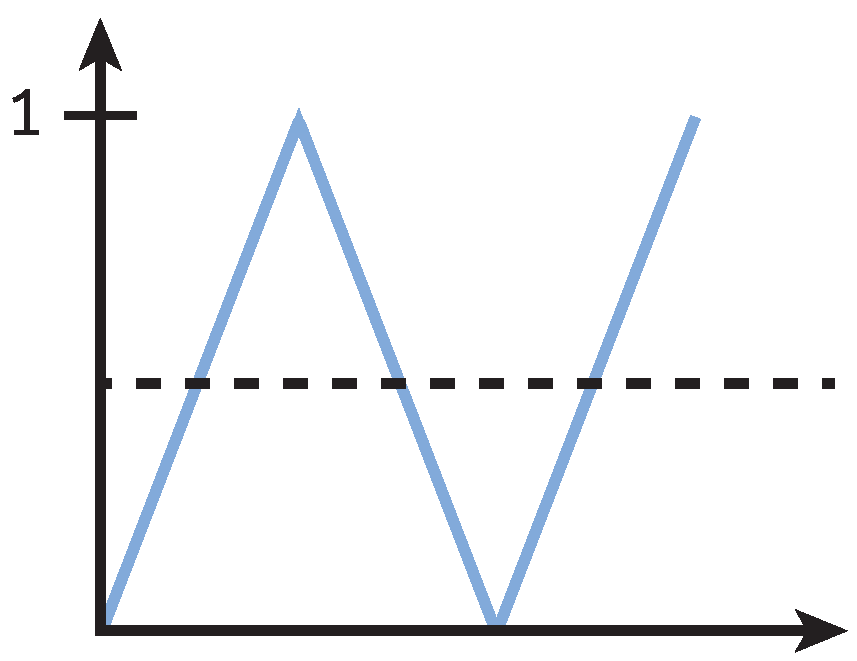
\includegraphics{FIGURES/total_variation}}
\caption[Illustration of a quantity fluctuating about a fixed point]{\label{fig:TV} Illustration of a quantity fluctuating between 0 and 1 about a fixed value.}
\end{center}
\end{figure}
We can compare the sum of the absolute value of the differences between the four points,
\begin{equation}\label{eq:sum_abs_tv}
\displaystyle \sum_{i=1}^{4}|Y(i+1)-Y(i)| = |1-0| + |0-1| + |1-0| = 3
\end{equation}
to the absolute value of the sum of the differences,
\begin{equation}\label{eq:abs_sum_tv}
|\displaystyle \sum_{i=1}^{4}(Y(i+1)-Y(i))| = |(1-0)+(0-1)+(1-0)| = 1
\end{equation}
The ratio of Eq.~(\ref{eq:sum_abs_tv}) and Eq.~(\ref{eq:abs_sum_tv}) is 3, which indicates that this data is fluctuating. For the implementation of this scheme in FDS, instead of comparing directly to 3, we use 2.9 because floating point division might not return a value of exactly 3. If fluctuations have been identified, then the values at the fourth point in the stencil are frozen and become the final values at the end of an integration time step. This prevents unnecessary sub-time steps being taken by the integrator. Because the error controller is bounding the solution, any one of the values within the stencil is also within the error tolerance and is therefore acceptable.


\chapter{Analytical Jacobian for Mixing and Detailed Chemistry}
\label{chemistry_analytical_jacobian}

The system of ODEs for concentration and temperature contains additional terms to account for turbulent mixing. Following the theory of Sec.~\ref{sec:subgrid_evironment}, we can derive these ODEs as follows.

\section{Mass Balance}
\label{mass_balance_mixing_chem}

Each cell in divided in two zones, unmixed and mixed.  Chemical reaction is only allowed in the mixed zone. The total mass in the cell is $\rho V_c$ where $V_c$ is the cell volume.  For the purposes of discussing the time integration for mixing and chemical kinetics, the variable $t$ here can be taken as zero at the start of an LES time step.  Thus, we are concerned with integration of the state of mixing and reaction within the cell from $0 \le t \le \delta t_{\mathrm{LES}}$.  The mass in the unmixed portion of the cell is $U(t)$ and the mass in the mixed zone is $M(t)$:
\begin{align} \label{eq:mixedAndUnmixedZoneMass}
\rho V_c &= U(t) + M(t) \\
U(t) &= \zeta(t) \rho V_c \\
M(t) &= (1-\zeta[t]) \rho V_c
\end{align}
Here, $\zeta(t)$ is the ``unmixed fraction'', which evolves by the following ODE:
\begin{equation}
\label{eq:zeta_copy}
\frac{\d \zeta}{\d t}=-\frac{\zeta}{\tau_{\rm mix}}
\end{equation}
with the solution{}
\begin{equation}
\label{eq:zeta_soln_copy}
\zeta(t) = \zeta_0 \,{\rm e}^{-t/\tau_{\rm mix}}
\end{equation}
where the state of mixing at the start of a CFD time step is $\zeta_0$ in this model.  In reality, the initial state of mixing in a computational cell obeys a transport equation, which itself requires modeling.  For present purposes we are choosing to set this value.  It can be shown that, if chemistry is infinitely fast, setting $\zeta_0=1$ corresponds to the basic ``eddy dissipation model'' or EDM.  Further, it can be shown \cite{FDS_Math_Guide} that Eq.~(\ref{eq:zeta_copy}) corresponds to a mixing model based on ``interaction by exchange with the \emph{mixed} mean'' or IEMM.  This model has the advantage over ``interaction by exchange with the mean '' or IEM \cite{Dopazo:1974}, which is often used in practical probability density function (PDF) models \cite{Pope:2000}, in that it avoids the issue of ``magical mixing'' across the reaction zone.

From Eqs.~(\ref{eq:mixedAndUnmixedZoneMass}), (\ref{eq:zeta_copy}), and (\ref{eq:zeta_soln_copy}), we can show
\begin{equation}
\label{eq:mixedzonemasstimederivative}
\frac{\d M}{\d t}= \frac{\zeta}{\tau_{\rm mix}} (\rho V_c) = \frac{\zeta}{(1-\zeta)\tau_{\rm mix}} M
\end{equation}

For the unmixed zone the mass fraction of species does not change with time. The mass fraction of $k$th species in the unmixed zone is $\widetilde{Y}_k^0$, same as the mean cell mass fraction at the beginning of the timestep. Let $\dot{m}_{k}^{'''}$ and $\dot{\omega}_k$ denote, respectively, the mass and molar time rate of change of species $k$ per unit volume. Similar to Eq.~(\ref{eq:mixmass}), using Eq.~(\ref{eq:mixedzonemasstimederivative}), we can derive an equation for the rate of change of mass of the $k$th species in the mixed zone as:
\begin{align} \label{eq:jspeciesmass}
    \frac{\d {\hat{m}_{k}}}{\d t} &= \dot{m}'''_{k} \hat{V} + \dot{m}_{k,in} \\
    &=\dot{\omega}_k W_k \hat{V} + \widetilde{Y}_k^0 \frac{\d M}{\d t} \\
    &=\dot{\omega}_k W_k \hat{V} + \widetilde{Y}_k^0 \frac{\zeta}{\tau_{\rm mix}} (\rho V_c)   \\
    &=\dot{\omega}_k W_k \hat{V} + \widetilde{Y}_k^0 \frac{\zeta}{(1-\zeta)\tau_{\rm mix}} M
\end{align}
Here the first term on the right hand side is due to chemistry, and second term is due to transfer of mass from unmixed zone to mixed zone. The Eqs.~(\ref{eq:mixedAndUnmixedZoneMass}), (\ref{eq:zeta_copy}), and (\ref{eq:zeta_soln_copy}) are used to derive this equation.


Now, using Eqs.~(\ref{eq:jspeciesmass}) and (\ref{eq:mixedzonemasstimederivative}), the change of mass fraction of the $k$th species in the mixed zone can be derived as follows:
\begin{align} \label{eq:jspeciesmassfraction}
    \hat{Y}_{k} &= \frac{\hat{m}_{k}}{M} \\
    \frac{\d {\hat{Y}_{k}}}{\d t} &= \frac{M \frac{\d {\hat{m}_{k}}}{\d t} - \hat{m}_{k} \frac{\d M}{\d t}}{M^2} \\
    &=\frac{1}{M} \left( \dot{\omega}_k W_k \hat{V} + \widetilde{Y}_k^0 \frac{\zeta}{(1-\zeta)\tau_{\rm mix}} M - \hat{Y}_{k} \frac{\d {M}}{\d t} \right)  \\
    &= \frac{\dot{\omega}_k W_k}{\hat{\rho}} + \left( \widetilde{Y}_k^0 - \hat{Y}_{k}\right) \frac{\zeta}{(1-\zeta) \tau_{\rm mix}}
\end{align}

Using Eq.~(\ref{eq:jspeciesmass}), the change of molar concentration of the $k$th species in the mixed zone can be derived as follows:
\begin{align} \label{eq:jspeciemolarconcentration}
    \hat{C}_{k} &= \frac{\hat{m}_{k}}{W_k \hat{V}} \\
    \frac{\d {\hat{C}_{k}}}{\d t} &= \frac{1}{W_k} \frac{\hat{V} \frac{\d {\hat{m}_{k}}}{\d t} - \hat{m}_{k} \frac{\d {\hat{V}}}{\d t}}{V^2_{mix}} \\
    &=\frac{1}{W_k \hat{V}} \left( \dot{\omega}_k W_k \hat{V} + \widetilde{Y}_k^0 \frac{\zeta}{(1-\zeta)\tau_{\rm mix}} M \right) - \hat{C}_{k} \frac{1}{\hat{V}}\frac{\d {\hat{V}}}{\d t}  \\
    &= \dot{\omega}_k +  \frac{\hat{\rho} \widetilde{Y}_k^0}{W_k} \frac{\zeta}{(1-\zeta) \tau_{\rm mix}} - \hat{C}_{k} \frac{1}{\hat{V}}\frac{\d {\hat{V}}}{\d t}
\end{align}

Again using Eq.~(\ref{eq:jspeciesmass}), the change of number of moles of the $k$th species in the mixed zone can be derived as follows:

\begin{align} \label{eq:jspeciesmole}
    \hat{N}_{k} &= \frac{\hat{m}_{k}}{W_k} \\
    \frac{\d {\hat{N}_{k}}}{\d t} &= \frac{1}{W_k} \frac{\d {\hat{m}_{k}}}{\d t} \\
    &= \frac{1}{W_k} \left( \dot{\omega}_k W_k \hat{V} + \widetilde{Y}_k^0 \frac{\zeta}{(1-\zeta)\tau_{\rm mix}} M \right)    \\
    &=\dot{\omega}_k \hat{V} + \frac{\widetilde{Y}_k^0}{W_k} \frac{\zeta}{(1-\zeta)\tau_{\rm mix}} M
\end{align}


For a constant pressure process, from the ideal gas equation of state, using Eq.~(\ref{eq:jspeciesmole}), we can write:
\begin{align} \label{eq:volumeterm}
     P\hat{V} &= \left(\sum{\hat{N}_j}\right) R \hat{T} \\
     \frac{1}{\hat{V}}\frac{\d {\hat{V}}}{\d t} & = \frac{1}{\hat{V}} \frac{R}{P} \left[ \left(\sum{\hat{N}_j}\right) \frac{\d \hat{T}}{\d t} + \hat{T} \left(\sum{\frac{\d \hat{N}_j}{\d t}}\right) \right] \\
     &= \frac{\left(\sum{\hat{N}_j}\right) R}{P \hat{V}} \frac{\d \hat{T}}{\d t} + \frac{R \hat{T}}{P \hat{V}} \left(\sum{\frac{\d \hat{N}_j}{\d t}}\right) \\
     &=\frac{1}{\hat{T}} \frac{\d \hat{T}}{\d t} + \frac{\left(\sum{\frac{\d \hat{N}_j}{\d t}}\right)}{\left(\sum{\hat{N}_j}\right)} \\
     & = \frac{1}{\hat{T}} \frac{\d \hat{T}}{\d t} + \frac{1}{\left(\sum{\hat{N}_j}\right)} \left[ \sum{\left(\dot{\omega}_j \hat{V} + \frac{\widetilde{Y}_j^0}{W_j} \frac{\zeta}{(1-\zeta)\tau_{\rm mix}} M \right) }\right]  \\
     &= \frac{1}{\hat{T}} \frac{\d \hat{T}}{\d t} + \frac{\sum{\dot{\omega}_j}}{\sum{\hat{C}_j}}+\frac{\zeta}{(1-\zeta)\tau_{\rm mix}}\sum{\frac{\hat{W}}{W_j} \widetilde{Y}_j^0} \\
     &= \frac{1}{\hat{T}} \frac{\d \hat{T}}{\d t} + \frac{\sum{\dot{\omega}_j}}{\sum{\hat{C}_j}}+\frac{\zeta}{(1-\zeta)\tau_{\rm mix}}\frac{\hat{W}}{\widetilde{W}^0}
\end{align}
Here $\hat{W}$ and $\widetilde{W}^0$ are the molecular weights of the mixed and unmixed zones, respectively.

Applying Eq.~(\ref{eq:volumeterm}) to Eq.~(\ref{eq:jspeciemolarconcentration}):
\begin{align} \label{eq:jspeciemolarconcentration2}
    \frac{\d {\hat{C}_{k}}}{\d t} &= \dot{\hat{C}}_k = \dot{\omega}_k +  \frac{\hat{\rho} \widetilde{Y}_k^0}{W_k} \frac{\zeta}{(1-\zeta) \tau_{\rm mix}} - \hat{C}_{k} \left[ \frac{1}{\hat{T}} \frac{\d \hat{T}}{\d t} + \frac{\sum{\dot{\omega}_j}}{\sum{\hat{C}_j}}+\frac{\zeta}{(1-\zeta)\tau_{\rm mix}}\frac{\hat{W}}{\widetilde{W}^0} \right]
\end{align}

Deatails of chemistry source term $\dot{{\omega}_k}$ can be found in Section \ref{chem_source_term}.

\section{Energy Balance}
\label{energy_balance_mixing_chem}

Now consider the total internal energy balance in the mixing zone:

\begin{align} \label{eq:mixedenergy}
    \frac{\d (M \hat{u}) }{\d t} &= \dot{m}_{in} \widetilde{h}^0 - \dot{W}_{pv} \\
    M \frac{\d  \hat{u} }{\d t} + \hat{u}\frac{\d  M }{\d t} &= \frac{\d  M }{\d t} \widetilde{h}^0 - P \frac{\d \left(M \hat{v} \right)}{\d t}
\end{align}

Here, $\dot{W}_{pv}$ is the work done by the mixed zone under constant pressure process, $\hat{u}$ is the specific internal energy of the mixed zone, $\widetilde{h}^0 \equiv \sum h_j(\widetilde{T}) \widetilde{Y}_j^0$ is the specific enthalpy of the unmixed zone, $\hat{v} = 1/\hat{\rho}$ is specific volume of the mixed zone.

Considering specific enthalpy of the mixed zone:
\begin{align} \label{eq:mixedinternalenergy}
    \hat{u}=\hat{h} - P\hat{v} = \hat{h} - \frac{P}{\hat{\rho}}
\end{align}


Applying Eq.~(\ref{eq:mixedinternalenergy}) to Eq.~(\ref{eq:mixedenergy}):

\begin{align} \label{eq:mixedenergy2}
     M \left[\frac{\d  \hat{h} }{\d t} -\cancel{P \frac{\d  \hat{v} }{\d t}} \right] + \hat{u}\frac{\d  M }{\d t} &= \frac{\d  M }{\d t} \widetilde{h}^0 - M \cancel{P \frac{\d  \hat{v} }{\d t}} - P \hat{v} \frac{\d  M }{\d t}\\
    \frac{\d  \hat{h} }{\d t} &= -\frac{1}{M} \frac{\d  M }{\d t} (\hat{u} -\widetilde{h}^0 - P \hat{v}) \\
    &= -\frac{\zeta}{(1-\zeta) \tau_{\rm mix}} (\hat{h} - \widetilde{h}^0)
\end{align}

Now writing the specific enthalpy as sum of the species specific enthalpy:
\begin{align} \label{eq:mixedenthalpy}
    \hat{h} &= \sum{\hat{Y}_j \hat{h}_j} \quad ; \quad \hat{h}_j \equiv h_j(\hat{T}) \\
    \frac{\d  \hat{h}}{\d t} &= \sum{ \left(\hat{Y}_j \frac{\d  \hat{h}_{j} }{\d t} \right) } + \sum{\left( \hat{h}_j \frac{\d  \hat{Y}_j }{\d t} \right)}
\end{align}

Using $\frac{\d  h_{j} }{\d t} = \hat{C}_{p,j} \frac{\d  T }{\d t}$, where $\hat{C}_{p,j}$ is the specific heat of species $j$, with Eq.~(\ref{eq:jspeciesmassfraction}) above we get,
\begin{align} \label{eq:mixedenthalpy2}
    \frac{\d  \hat{h} }{\d t} &= \frac{\d \hat{T}}{\d t} \sum{\left(\hat{Y}_j \hat{C}_{p,j} \right)} + \sum{\left(\hat{h}_j \frac{\d  \hat{Y}_j }{\d t} \right)} \\
    &=\hat{c}_p \frac{\d \hat{T}}{\d t} + \sum{\hat{h}_j \left(\frac{\dot{\omega}_j W_j}{\hat{\rho}} + \left( \widetilde{Y}_j^0 - \hat{Y}_j\right) \frac{\zeta}{(1-\zeta) \tau_{\rm mix}} \right)}
\end{align}

Now, equating Eq. \ref{eq:mixedenthalpy2} with Eq. \ref{eq:mixedenergy2}:

\begin{align} \label{eq:tempeqn}
 \frac{\d \hat{T} }{\d t} &= \dot{\hat{T}} = -\frac{1}{\hat{\rho} \hat{c}_p} (\underbrace{\sum \hat{h}_j W_j \dot{\omega}_j}_{\dot{q}'''} - \dot{q}_{\rm loss}^{'''})  -  \frac{\zeta}{(1-\zeta) \tau_{\rm mix}} \frac{1}{\hat{c}_p}  \left[ \cancel{\hat{h}} - \widetilde{h}^0 + \sum{\hat{h}_j \widetilde{Y}_j^0} - \cancel{\sum{\hat{h}_j \hat{Y}_j}} \right] \\
 &=-\frac{1}{\hat{\rho} \hat{c}_p} \left[ \dot{q}''' (1-\chi_{\rm loss}) +  \frac{\zeta}{(1-\zeta) \tau_{\rm mix}}  \left( \hat{\rho} \sum{(\hat{h}_j \widetilde{Y}_j^0)} - \hat{\rho} \widetilde{h}^0 \right) \right]
\end{align}
Here, $\chi_{\rm loss}$ can be considered a radiation loss fraction if known \emph{a priori}.

Eqs.~(\ref{eq:jspeciemolarconcentration2}) and (\ref{eq:tempeqn}) will be used in CVODE as the ODE RHS.

Deatails of chemistry source term $\dot{{\omega}_j}$ can be found in Section \ref{chem_source_term}.


\section{Analytical Jacobian formulation}
\label{jacobian_mixing_chem}

Providing an analytical Jacobian to the CVODE solver can significantly accelerate the chemistry calculations. The Jacobian for the given system can be written as:

\begin{align}
J &=
\begin{bmatrix}
\frac{\partial\dot{\hat{C}}_{1}}{\partial \hat{C}_{1}}& \frac{\partial \dot{\hat{C}}_{2}}{\partial \hat{C}_{1}} & \ldots & \frac{\partial \dot{\hat{C}}_{N_{\rm s}}}{\partial \hat{C}_{1}} & | & \frac{\partial \dot{\hat{T}}}{\partial \hat{C}_{1}}\\
\frac{\partial\dot{\hat{C}}_{1}}{\partial \hat{C}_{2}}& \frac{\partial \dot{\hat{C}}_{2}}{\partial \hat{C}_{2}} & \ldots & \frac{\partial \dot{\hat{C}}_{N_{\rm s}}}{\partial \hat{C}_{2}} & | &\frac{\partial \dot{\hat{T}}}{\partial \hat{C}_{2}}\\
\ldots & \ldots & \ldots & \ldots & | & \ldots\\
\frac{\partial \dot{\hat{C}}_{1}}{\partial \hat{C}_{N_{\rm s}}}& \frac{\partial \dot{\hat{C}}_{2}}{\partial \hat{C}_{N_{\rm s}}} & \ldots & \frac{\partial \dot{\hat{C}}_{N_{\rm s}}}{\partial \hat{C}_{N_{\rm s}}} & | & \frac{\partial \dot{\hat{T}}}{\partial \hat{C}_{N_{\rm s}}}\\
---& --- & --- & --- & | & ---\\
\frac{\partial \dot{\hat{C}}_{1}}{\partial \hat{T}}& \frac{\partial \dot{\hat{C}}_{2}}{\partial \hat{T}} & \ldots & \frac{\partial \dot{\hat{C}}_{N_{\rm s}}}{\partial \hat{T}} & | & \frac{\partial \dot{\hat{T}}}{\partial \hat{T}}\\
\end{bmatrix}
=\begin{bmatrix}
\frac{\partial \boldsymbol{\dot{\hat{C}}}}{\boldsymbol{\partial \hat{C}}}& \frac{\partial \dot{\hat{T}}}{\partial \boldsymbol{\hat{C}}}\\
\frac{\partial \boldsymbol{\dot{\hat{C}}}}{\partial \hat{T}}& \frac{\partial \dot{\hat{T}}}{\partial \hat{T}}
\end{bmatrix}
\label{eq:jacobian_mix_chem}
\end{align}


\begin{align} \label{eq:jspeciemolarconcentration3}
    \frac{\d {\hat{C}_{k}}}{\d t} &= \dot{\hat{C}}_k = \underbrace{\dot{\omega}_k}_{\dot{\hat{C}}_{k,A}}
    + \underbrace{\frac{\hat{\rho} \widetilde{Y}_k^0}{W_k} \frac{\zeta}{(1-\zeta) \tau_{\rm mix}}}_{\dot{\hat{C}}_{k,B}}
    - \underbrace{\hat{C}_{k} \left[ \frac{1}{\hat{T}} \frac{\d \hat{T}}{\d t} + \frac{\sum{\dot{\omega}_j}}{\sum{\hat{C}_j}}+\frac{\zeta}{(1-\zeta)\tau_{\rm mix}}\frac{\hat{W}}{\widetilde{W}^0} \right] }_{\dot{\hat{C}}_{k,C}}
\end{align}

\begin{align} \label{eq:jspeciemolarconcentration4}
   \boldsymbol{\dot{\hat{C}}} = \boldsymbol{\dot{\hat{C}}_A}+\boldsymbol{\dot{\hat{C}}_B} + \boldsymbol{\dot{\hat{C}}_C}
\end{align}

\begin{align} \label{eq:tempeqn2}
 \frac{\d \hat{T} }{\d t} &= \dot{\hat{T}} = \underbrace{-\frac{1}{\hat{\rho} \hat{c}_p} \sum{\hat{h}_j W_j \dot{\omega}_j }}_{\dot{\hat{T}}_A}
 -  \underbrace{\frac{\zeta}{(1-\zeta) \tau_{\rm mix}} \frac{1}{\hat{c}_p}  \left[ \sum{\hat{h}_j \widetilde{Y}_j^0} - \widetilde{h}^0 \right]}_{\dot{\hat{T}}_B}
\end{align}

\begin{align} \label{eq:tempeqn4}
   \boldsymbol{\dot{\hat{T}}} = \boldsymbol{\dot{\hat{T}}_A}+\boldsymbol{\dot{\hat{T}}_B}
\end{align}

\subsection*{Calculation of $\frac{\partial \boldsymbol{\dot{\hat{C}}_A}}{\mathbf{\partial \hat{C}}}$}
Here, $\dot{\hat{C}}_{k,A} = \dot{\omega}_{k}$. This term can be be calculated using Eq. \ref{eq:Jac1st} detailed in Section \ref{chem_source_term}.

\subsection*{Calculation of $\frac{\partial \boldsymbol{\dot{\hat{C}}_B}}{\mathbf{\partial \hat{C}}}$}

\begin{align}\label{eq:JacCBC}
\frac{\partial \dot{\hat{C}}_{k,B}}{\partial \hat{C}_{l}} &= \frac{W_l}{W_k} \frac{\zeta}{(1-\zeta) \tau_{\rm mix}} \widetilde{Y}_k^0
\end{align}
Here, we used the relation, $\frac{\partial \hat{\rho}}{\partial \hat{C}_{l}} = W_l$.

\subsection*{Calculation of $\frac{\partial \boldsymbol{\dot{\hat{C}}_C}}{\mathbf{\partial \hat{C}}}$}
\begin{align}\label{eq:JacCCC}
\frac{\partial \dot{\hat{C}}_{k,C}}{\partial \hat{C}_{l}} &= - \delta_{lk} \left[ \frac{1}{\hat{T}} \frac{\d \hat{T}}{\d t} + \frac{\sum{\dot{\omega}_j}}{\sum{\hat{C}_j}}+\frac{\zeta}{(1-\zeta)\tau_{\rm mix}}\frac{\hat{W}}{\widetilde{W}^0} \right] \notag\\
&- \hat{C}_{k} \left[ \frac{\partial}{\partial \hat{C}_{l}} \left( \frac{1}{\hat{T}} \frac{\d \hat{T}}{\d t} \right) + \frac{\partial}{\partial \hat{C}_{l}} \left( \frac{\sum{\dot{\omega}_j}}{\sum{\hat{C}_j}}\right) + \frac{\zeta}{(1-\zeta)\tau_{\rm mix}} \frac{\partial}{\partial \hat{C}_{l}} \left( \frac{\hat{W}}{\widetilde{W}^0} \right)\right]
\end{align}

Now calculate each of the individual terms of the second line.
\begin{align}\label{eq:dTempByDConc}
\frac{\partial \hat{T}}{\partial \hat{C}_{l}} &= \frac{\partial \left(\frac{P}{R \sum{\hat{C}_j}} \right) }{\partial \hat{C}_{l}} \\
&= -\frac{P\sum{\delta_{jl}}}{R \left(\sum{\hat{C}_j}\right)^2}
= - \frac{\hat{T}\sum{\delta_{jl}}}{\sum{\hat{C}_j}}
= - \frac{\hat{T}}{\sum{\hat{C}_j}} \quad ; \quad \text{since $\sum{\delta_{jl}}$ =1}
\end{align}

\begin{align}\label{eq:JacCCC_1}
\frac{\partial}{\partial \hat{C}_{l}} \left( \frac{1}{\hat{T}} \frac{\d \hat{T}}{\d t} \right)&= \frac{1}{\hat{T}} \frac{\partial}{\partial \hat{C}_{l}} \left( \frac{\d \hat{T}}{\d t} \right) - \frac{1}{\hat{T}^2} \frac{\d \hat{T}}{\d t} \frac{\partial \hat{T}}{\partial \hat{C}_{l}} \\
&= \frac{1}{\hat{T}} \frac{\partial}{\partial \hat{C}_{l}} \left( \frac{\d \hat{T}}{\d t} \right) + \frac{1}{\hat{T}} \frac{\d \hat{T}}{\d t} \frac{1}{\sum{\hat{C}_j}} \\
&=\frac{1}{\hat{T}} \left[ \frac{\partial}{\partial \hat{C}_{l}} \left( \frac{\d \hat{T}}{\d t} \right) + \frac{1}{\sum{\hat{C}_j}} \frac{\d \hat{T}}{\d t} \right]
\end{align}

\begin{align}\label{eq:JacCCC_2}
\frac{\partial}{\partial \hat{C}_{l}} \left( \frac{\sum{\dot{\omega}_j}}{\sum{\hat{C}_j}}\right) &= \frac{1}{\sum{\hat{C}_j}} \sum{\left(\frac{\partial \dot{\omega}_j}{\partial \hat{C}_{l}} \right)} - \frac{\sum{\delta_{jl}}}{\sum{(\hat{C}_j)}^2} \sum{\dot{\omega}_j} \\
&= \frac{1}{\sum{\hat{C}_j}} \left[ \sum{\left(\frac{\partial \dot{\omega}_j}{\partial \hat{C}_{l}} \right)} - \frac{\sum{\dot{\omega}_j}}{\sum{(\hat{C}_j)}}  \right]
\end{align}


\begin{align}\label{eq:JacCCC_3}
\frac{\zeta}{(1-\zeta)\tau_{\rm mix}} \frac{\partial}{\partial \hat{C}_{l}} \left( \frac{\hat{W}}{\widetilde{W}^0} \right) &= \frac{\zeta}{(1-\zeta)\tau_{\rm mix} \widetilde{W}^0} \frac{\partial}{\partial \hat{C}_{l}} \left( \frac{\sum{\hat{C}_j W_j}}{\sum{\hat{C}_j}} \right) \\
&=\frac{\zeta}{(1-\zeta)\tau_{\rm mix} \widetilde{W}^0 \left(\sum{\hat{C}_j} \right)} \left(W_l-\hat{W} \right)
\end{align}


\subsection*{Calculation of $\frac{\partial \boldsymbol{\dot{\hat{C}}_A}}{\partial \hat{T}}$}
\begin{align}\label{eq:JacCAT}
\frac{\partial {\dot{\hat{C}}_{k,A}}}{\partial \hat{T}} = \frac{\partial \dot{\omega}_k}{\partial \hat{T}}
\end{align}
This term can be be calculated using Eq. \ref{eq:Jac2nd} detailed in Section \ref{chem_source_term}.




\subsection*{Calculation of $\frac{\partial \boldsymbol{\dot{\hat{C}}_B}}{\partial \hat{T}}$}
\begin{align}\label{eq:JacCBT}
\frac{\partial {\dot{\hat{C}}_{k,B}}}{\partial \hat{T}} = - \frac{\hat{\rho}}{\hat{T} W_k} \frac{\zeta}{(1-\zeta) \tau_{\rm mix}} \widetilde{Y}_k^0
\end{align}
Here the relation $\frac{\partial \hat{\rho}}{\partial \hat{T}} = -\frac{\hat{\rho}}{\hat{T}}$ is used.

\subsection*{Calculation of $\frac{\partial \boldsymbol{\dot{\hat{C}}_C}}{\partial \hat{T}}$}

\begin{align}\label{eq:JacCCT}
\frac{\partial {\dot{\hat{C}}_{k,C}}}{\partial \hat{T}} &= - \frac{\partial \hat{C}_{k}}{\partial \hat{T}} \left[ \frac{1}{\hat{T}} \frac{\d \hat{T}}{\d t} + \frac{\sum{\dot{\omega}_j}}{\sum{\hat{C}_j}}+\frac{\zeta}{(1-\zeta)\tau_{\rm mix}}\frac{\hat{W}}{\widetilde{W}^0} \right] \notag\\
& - \hat{C}_{k} \left[ \frac{\partial}{\partial \hat{T}} \left( \frac{1}{\hat{T}} \frac{\d \hat{T}}{\d t} \right) + \frac{\partial}{\partial \hat{T}} \left( \frac{\sum{\dot{\omega}_j}}{\sum{\hat{C}_j}}\right) + \frac{\zeta}{(1-\zeta)\tau_{\rm mix}} \frac{\partial}{\partial \hat{T}} \left( \frac{\hat{W}}{\widetilde{W}^0} \right)\right] \\
&= \frac{\hat{C}_{k}}{\hat{T}} \left[ \frac{1}{\hat{T}} \frac{\d \hat{T}}{\d t} + \cancel{\frac{\sum{\dot{\omega}_j}}{\sum{\hat{C}_j}}}+\frac{\zeta}{(1-\zeta)\tau_{\rm mix}}\frac{\hat{W}}{\widetilde{W}^0} \right] \notag\\
& - \hat{C}_{k} \left [ \left[ \frac{1}{\hat{T}} \frac{\partial}{\partial \hat{T}} \left( \frac{\d \hat{T}}{\d t} \right) - \frac{1}{\hat{T}^2} \frac{\d \hat{T}}{\d t} \right] + \left[\frac{1}{\sum{\hat{C}_j}} \sum{\frac{\partial \dot{\omega}_j}{\partial \hat{T}}} + \cancel{\frac{\sum{\dot{\omega}_j}}{\left(\sum{\hat{C}_j}\right)^2} \sum{\frac{\hat{C}_j}{\hat{T}}}} \right] \right. \notag\\
&+  \left. \left[\frac{\zeta}{(1-\zeta)\tau_{\rm mix}\widetilde{W}^0} \frac{\partial}{\partial \hat{T}} \left( \frac{\sum{\hat{C}_j W_j}}{\sum{\hat{C}_j}} \right) \right] \right] \\
&= - \hat{C}_{k} \left[ \frac{1}{\hat{T}} \frac{\partial}{\partial \hat{T}} \left( \frac{\d \hat{T}}{\d t} \right) + \frac{1}{\sum{\hat{C}_j}} \sum{\frac{\partial \dot{\omega}_j}{\partial \hat{T}}} - \frac{2}{\hat{T}^2}\frac{\d \hat{T}}{\d t}\right]
\end{align}

It can be shown that $\frac{\partial \hat{W}}{\partial \hat{T}} = \frac{\partial}{\partial \hat{T}} \left( \frac{\sum{\hat{C}_j W_j}}{\sum{\hat{C}_j}} \right) = 0 $. Here, the relation $\frac{\partial \hat{C}_j}{\partial \hat{T}} = - \frac{\hat{C}_j}{\hat{T}}$ is used.


\subsection*{Calculation of $\frac{\partial \dot{\hat{T}}_A}{\mathbf{\partial \hat{C}}}$}
\begin{align}\label{eq:JacTAC}
\frac{\partial {\dot{\hat{T}}_{k,A}}}{\partial \hat{C}_{l}} = \frac{\partial}{\partial \hat{C}_{l}} \left( -\frac{1}{\hat{\rho} \hat{c}_p} \sum{\hat{h}_j W_j \dot{\omega}_j }\right)
\end{align}
This term can be be calculated using Eq. \ref{eq:Jac3rd} detailed in Section \ref{chem_source_term}.

\subsection*{Calculation of $\frac{\partial \dot{\hat{T}}_B}{\mathbf{\partial \hat{C}}}$}
\begin{align}\label{eq:JacTBC}
\frac{\partial {\dot{\hat{T}}_{k,B}}}{\partial \hat{C}_{l}} &= - \frac{\zeta}{(1-\zeta) \tau_{\rm mix}} \left[\left( \sum{\hat{h}_j \widetilde{Y}_j^0} - \widetilde{h}^0 \right) \frac{1}{\left(\hat{c}_p\right)^2} \frac{W_l}{\hat{\rho}} \left( \hat{c}_p - \hat{C}_{p,l}\right)   \right] \\
&= - \frac{\zeta}{(1-\zeta) \tau_{\rm mix}} \frac{W_l}{\hat{\rho} \hat{c}_p} \left[ \left( \sum{\hat{h}_j \widetilde{Y}_j^0} - \widetilde{h}^0 \right) \frac{\left( \hat{c}_p - \hat{C}_{p,l}\right)}{\hat{c}_p} \right]
\end{align}
The relation $\frac{\partial \hat{c}_p}{\partial \hat{C}_{l}} = - \frac{W_l}{\hat{\rho}}\left( \hat{c}_p -\hat{C}_{p,l} \right)$ is used here.

\subsection*{Calculation of $\frac{\partial \dot{\hat{T}}_A}{\partial \hat{T}}$}
\begin{align}\label{eq:JacTAT}
\frac{\partial {\dot{\hat{T}}_{k,A}}}{\partial \hat{T}} = \frac{\partial}{\partial \hat{T}} \left( -\frac{1}{\hat{\rho} \hat{c}_p} \sum{\hat{h}_j W_j \dot{\omega}_j }\right)
\end{align}
This term can be be calculated using Eq. \ref{eq:Jac4th} detailed in Section \ref{chem_source_term}.

\subsection*{Calculation of $\frac{\partial \dot{\hat{T}}_B}{\partial \hat{T}}$}

\begin{align}\label{eq:JacTBT}
\frac{\partial {\dot{\hat{T}}_{k,B}}}{\partial \hat{T}} &= - \frac{\zeta}{(1-\zeta) \tau_{\rm mix}} \left[\frac{1}{\hat{c}_p}  \left( \sum{\hat{C}_{p,j}\widetilde{Y}_j^0} \right)
+ \left( \sum{\hat{h}_j \widetilde{Y}_j^0} - \widetilde{h}^0 \right) \frac{1}{\left(\hat{c}_p\right)^2} \frac{\partial \hat{c}_p}{\partial \hat{T}}   \right] \\
&= - \frac{\zeta}{(1-\zeta) \tau_{\rm mix}} \frac{1}{\hat{c}_p} \left[ \sum{\hat{C}_{p,j}\widetilde{Y}_j^0} + \frac{1}{\hat{c}_p}\left( \sum{\hat{h}_j \widetilde{Y}_j^0} - \widetilde{h}^0 \right) \frac{\partial \hat{c}_p}{\partial \hat{T}}  \right]
\end{align}

\section{Chemistry Source Term Calculation}
\label{chem_source_term}

The system of ODEs to solve a detailed chemical mechanism is given by Eqs.~(\ref{eq:chemistry_ode_system}) and (\ref{eq:TemperatureDerivative})
\begin{equation}\label{eq:chemistry_ode_system_appendix}
\frac{\d C_k}{\d t} =  \dot{\omega}_k = \sum_{i=1}^{N_{\rm r}} b_i \ \nu_{ki} \ r_i,  j=1,2,3,...,N_{\rm s}
\end{equation}
\begin{equation}\label{eq:TemperatureDerivativeAppendix}
\frac{\d T}{\d t} = \dot{T} = -\frac{1}{\rho c_p} \sum_{j=1}^{N_{\rm s}}h_j W_j \dot{\omega}_j
\end{equation}
For Eq.~(\ref{eq:chemistry_ode_system_appendix}), $C_j$ is the molar concentration \si{(kmol/m^3)} of the $j$th species; $b_i$ is the reaction rate modification coefficient of the $i$th reaction due to third-body effects and pressure; $\nu_{ki} = {\nu}_{ki}^{''} - {\nu}_{ki}^{'}$; and $r_i$ is the reaction progress rate of the $i$th reaction.
\begin{equation}\label{eq:reaction_progress_rate_appendix}
r_i =  k_{f,i} \prod_{j=1}^{N_{\rm s}} (C_j)^{{\nu}_{ji}^{'}}  -  k_{r,i} \prod_{j=1}^{N_{\rm s}} (C_j)^{{\nu}_{ji}^{''}}
\end{equation}
For Eq.~(\ref{eq:TemperatureDerivativeAppendix}), $\rho$  is the density \si{(kg/m^3)}, $c_p$ is the specific heat of the mixture (J/kg/K), $h_k$ is the absolute enthalpy that includes enthalpy of formation (J/kg), $W_j$ is the molecular weight (kg/kmol) of species $j$, and $\dot{\omega}$ is the species production rate given by Eq.~(\ref{eq:chemistry_ode_system_appendix}).

The system of ODEs can be represented by:
\be
\begin{aligned}
f &= \left[ \frac{\d C_1}{\d t} \ \frac{\d C_2}{\d t} \ldots \ \frac{\d C_{N_{\rm s}}}{\d t} \ \frac{\d T}{\d t} \right]^T \
  &= \left[  \dot{\omega}_1 \ \dot{\omega}_2 \ldots \ \dot{\omega}_{N_{\rm s}} \ \dot{T} \right]^T \
\end{aligned}
\ee

Providing an analytical Jacobian to the CVODE solver can significantly accelerate the chemistry calculations. The Jacobian for the given system can be written as:
\be
\begin{aligned}
J &=
\begin{bmatrix}
\frac{\partial\dot{\omega}_1}{\partial C_1}& \frac{\partial \dot{\omega}_2}{\partial C_1} & \ldots & \frac{\partial \dot{\omega}_{N_{\rm s}}}{\partial C_1} & | & \frac{\partial \dot{T}}{\partial C_1}\\
\frac{\partial\dot{\omega}_1}{\partial C_2}& \frac{\partial \dot{\omega}_2}{\partial C_2} & \ldots & \frac{\partial \dot{\omega}_{N_{\rm s}}}{\partial C_2} & | &\frac{\partial \dot{T}}{\partial C_2}\\
\ldots & \ldots & \ldots & \ldots & | & \ldots\\
\frac{\partial \dot{\omega}_1}{\partial C_{N_{\rm s}}}& \frac{\partial \dot{\omega}_2}{\partial C_{N_{\rm s}}} & \ldots & \frac{\partial \dot{\omega}_{N_{\rm s}}}{\partial C_{N_{\rm s}}} & | & \frac{\partial \dot{T}}{\partial C_{N_{\rm s}}}\\
---& --- & --- & --- & | & ---\\
\frac{\partial \dot{\omega}_1}{\partial T}& \frac{\partial \dot{\omega}_2}{\partial T} & \ldots & \frac{\partial \dot{\omega}_{N_{\rm s}}}{\partial T} & | & \frac{\partial \dot{T}}{\partial T}\\
\end{bmatrix}
&=\begin{bmatrix}
\frac{\partial \mathbf{\dot{\omega}}}{\mathbf{\partial C}}& \frac{\partial \dot{T}}{\partial \mathbf{C}}\\
\frac{\partial \mathbf{\dot{\omega}}}{\partial T}& \frac{\partial \dot{T}}{\partial T}
\end{bmatrix}
\label{eq:jacobian_chem}
\end{aligned}
\ee

This Jacobian is the first part of equations \ref{eq:jspeciemolarconcentration3} and \ref{eq:tempeqn2} for the mixing and chemistry Jacobian matrix (\ref{eq:jacobian_mix_chem}).

\subsection*{Calculation of $\frac{\partial \mathbf{\dot{\omega}}}{\mathbf{\partial C}}$}
By taking derivative of Eq.~(\ref{eq:chemistry_ode_system_appendix}) with respect to concentration, we can write:
\begin{equation}\label{eq:Jac1st}
\begin{aligned}
\frac{\partial \dot{\omega}_k}{\partial C_l} &= \sum_{i=1}^{N_{reac}} \left[ \nu_{ki} \ r_i \ \frac{\partial b_i}{\partial C_l} +  b_i \nu_{ki} \  \left( k_{f,i} \nu_{li}^{'} \ \frac{\prod_{j=1}^{N_{\rm s}} (C_j)^{{\nu}_{ji}^{'}} }{C_l}  -  k_{r,i} \ \nu_{li}^{''} \ \frac{\prod_{j=1}^{N_{\rm s}} (C_j)^{{\nu}_{ji}^{''}} }{C_l} \right) \right],
\end{aligned}
\end{equation}
Here, the $\frac{\partial b_i}{\partial C_l}$ term can be calculated using Eqs.~(\ref{eq:reac_mod_coeff})-(\ref{eq:falloff_Fi}).

\subsection*{Calculation of $\frac{\partial \mathbf{\dot{\omega}}}{\partial T}$}
By taking derivative of Eq.~(\ref{eq:chemistry_ode_system_appendix}) with respect to temperature, we can write:
\begin{multline}\label{eq:Jac2nd}
\frac{\partial \dot{\omega}_k}{\partial T} = \sum_{i=1}^{N_{reac}} \left[ \nu_{ki} \ r_i \ \frac{\partial b_i}{\partial T} +  b_i \nu_{ki} \  \left\{  \frac{\partial k_{f,i}}{\partial T} \prod_{j=1}^{N_{\rm s}} (C_j)^{{\nu}_{ji}^{'}}  + k_{f,i} \frac{\partial}{\partial T} \left( \prod_{j=1}^{N_{\rm s}} (C_j)^{{\nu}_{ji}^{'}}  \right) \right. \right. \\
- \left. \left. \frac{\partial k_{r,i}}{\partial T} \prod_{j=1}^{N_{\rm s}} (C_j)^{{\nu}_{ji}^{''}}  - k_{r,i} \frac{\partial}{\partial T} \left( \prod_{j=1}^{N_{\rm s}} (C_j)^{{\nu}_{ji}^{''}}  \right) \right\} \right]
\end{multline}
Similar to $\frac{\partial b_i}{\partial C_l}$, $\frac{\partial b_i}{\partial T}$ can be calculated using Eqs.~(\ref{eq:reac_mod_coeff})-(\ref{eq:falloff_Fi}).
\begin{equation} \label{eq:kfTmpDerivative}
\frac{\partial k_{f,i}}{\partial T} = \frac{k_{f,i}}{T} \left( n_{f,i} + \frac{E_{a,i}}{RT} \right) \ \text{using Eq. \ref{eq:rate_cons}}
\end{equation}
\begin{equation}\label{eq:krTmpDerivative}
\begin{aligned}
\frac{\partial k_{r,i}}{\partial T} &= \frac{\partial}{\partial T} \left( \frac{k_{f,i}}{K_i}  \right) \
&= k_{r,i} \left( \frac{1}{k_{f,i}} \frac{\partial k_{f,i}}{\partial T} - \frac{1}{K_i} \frac{\partial K_i}{\partial T} \right)
\end{aligned}
\end{equation}
Here, $K_i$ is the concentration equilibrium constant obtained using Eq.~(\ref{eq:equilibrium_const}). Through mathematical derivation, it can be shown that:
\begin{equation}\label{eq:EqConstTmpDerivative}
\begin{aligned}
\frac{1}{K_i} \frac{\partial K_i}{\partial T} = -\frac{1}{T} \left( \sum_{i=1}^{N_{\rm s}} {\nu}_{ji}^{''} -  \sum_{i=1}^{N_{\rm s}} {\nu}_{ji}^{'}  \right) + \frac{1}{R T} \left(  \frac{\Delta G_{\mathrm{rxn}}}{T} + \Delta S_{\mathrm{rxn}}   \right)
\end{aligned}
\end{equation}
Here, $\Delta S_{\mathrm{rxn}}$ is the change in entropy, and can be calculated similar to the process described in Section \ref{sec:equilChem}.
\begin{equation}\label{eq:ConcTmpDerivative}
\begin{aligned}
\frac{\partial}{\partial T} \left( \prod_{j=1}^{N_{\rm s}} (C_j)^{{\nu}_{ji}^{'}}  \right) &= - \frac{1}{T} \left(  \sum_{j=1}^{N_{\rm s}} {\nu}_{ji}^{'} \right) \left(  \prod_{j=1}^{N_{\rm s}} (C_j)^{{\nu}_{ji}^{'}}  \right) \\
\frac{\partial}{\partial T} \left( \prod_{j=1}^{N_{\rm s}} (C_j)^{{\nu}_{ji}^{''}}  \right) &= - \frac{1}{T} \left(  \sum_{j=1}^{N_{\rm s}} {\nu}_{ji}^{''} \right) \left(  \prod_{j=1}^{N_{\rm s}} (C_j)^{{\nu}_{ji}^{''}}  \right){}
\end{aligned}
\end{equation}
In the above derivation, the relation $\frac{\partial C_j}{\partial T} = - \frac{C_j}{T}$ is used.
Using Eqs.~(\ref{eq:kfTmpDerivative})-(\ref{eq:ConcTmpDerivative}), all the terms of Eq.~(\ref{eq:Jac2nd}) can be calculated.


\subsection*{Calculation of $\frac{\partial \dot{T}}{\partial \mathbf{C}}$}
By taking derivative of Eq.~(\ref{eq:TemperatureDerivativeAppendix}) with respect to concentration, we can write:
\begin{equation} \label{eq:Jac3rd}
\begin{aligned}
\frac{\partial \dot{T}}{\partial C_l} &= \frac{\partial}{\partial C_l} \left( -\frac{1}{\rho c_p} \sum_{j=1}^{N_{\rm s}}h_j W_j \dot{\omega}_j  \right) \\
&= -\left( \frac{1}{\rho} \frac{\partial \rho}{\partial C_l} +  \frac{1}{c_p} \frac{\partial c_p}{\partial C_l} \right) \dot{T} - \frac{1}{{\rho} c_p} \sum_{j=1}^{N_{\rm s}}h_j W_j \frac{\partial \dot{\omega}_j}{\partial C_l}
\end{aligned}
\end{equation}
Using the relations $\frac{\partial \rho}{\partial C_l} = W_l$ and $\frac{\partial c_p}{\partial C_l} = - \frac{W_l}{\rho}\left( c_p -c_{p,l} \right)$, we can rewrite Eq. ~(\ref{eq:Jac3rd}) as:
\begin{equation} \label{eq:Jac3rd_final}
\frac{\partial \dot{T}}{\partial C_l} = \frac{W_l c_{p,l}}{\rho c_p} \dot{T} - \frac{1}{{\rho} c_p} \sum_{j=1}^{N_{\rm s}}h_j W_j \frac{\partial \dot{\omega}_j}{\partial C_l}
\end{equation}
Here, $c_{p,l}$ is the specific heat of species $l$. The last term Eq.~(\ref{eq:Jac3rd_final}) can be obtained using Eq. \ref{eq:Jac1st}.

\subsection*{Calculation of $\frac{\partial \dot{T}}{\partial T}$}
By taking derivative of Eq.~(\ref{eq:TemperatureDerivativeAppendix}) with respect to temperature, we can write:
\begin{equation} \label{eq:Jac4th}
\begin{aligned}
\frac{\partial \dot{T}}{\partial T} &= \frac{\partial}{\partial T} \left( -\frac{1}{\rho c_p} \sum_{j=1}^{N_{\rm s}}h_j W_j \dot{\omega}_j  \right) \\
&=\frac{\dot{T}}{T} - \frac{1}{c_p} \frac{\partial c_p}{\partial T} \dot{T} - \frac{1}{\rho c_p} \sum_{j=1}^{N_{\rm s}} \left[ h_j  \frac{\partial \dot{\omega}_j}{\partial T} +  \dot{\omega}_j c_{p,j} \right] W_j
\end{aligned}
\end{equation}
To derive the above equation, the relations $\frac{\partial \rho}{\partial T} = -\frac{\rho}{T}$ and $\frac{\partial h_j}{\partial T} = c_{p,j}$ are used. The term $\frac{\partial \dot{\omega}_j}{\partial T}$ can be obtained using Eq.~(\ref{eq:Jac2nd}).


\chapter{The Unmixed Fraction}
\label{app:unmixed_fraction}

In Sec.~\ref{sec:subgrid_evironment} we present the evolution equation for an important variable, the unmixed fraction, $\zeta$, in the batch reactor model for turbulent combustion.  This appendix explains the development of that equation.

\subsection*{Moments of the PDF Transport Equation}
\label{app:pdf_transport}

The cell mean mass fraction of species $\alpha$ is denoted $\widetilde{Y}_\alpha(t)$. A fluid parcel at any point within the cell exists in one of two states: completely unmixed or completely mixed.  Let $\hat{Y}_\alpha(t)$ denote the mass fraction of $\alpha$ in the mixed reactor zone, initially equal to the cell mean, $\hat{Y}_\alpha(0) = \widetilde{Y}_{\alpha}^0 \equiv \widetilde{Y}_{\alpha}(0)$.  With $\psi_\alpha \in [0,1]$ representing the sample space for the composition, the subgrid probability density function (PDF) may be written as
\begin{equation}
\label{eq:pdf}
f(\psi_\alpha;t) = w_1 \delta(0-\psi_\alpha) + w_2 \delta(1-\psi_\alpha) + w_3 \delta(\hat{Y}_\alpha[t] - \psi_\alpha)
\end{equation}
where $\delta(x)$ is the Dirac delta function.  In other words, if we look at a specific point, the mass fraction of species $\alpha$ may only be 0, 1, or equal to the mixed zone value, $\hat{Y}_\alpha$ (see Fig.~\ref{fig_subgrid_environment}).  The weights $w_i$ must satisfy integral constraints on the cell: $\int f(\psi_\alpha;t) \d \psi_\alpha = 1$, $\int f(\psi_\alpha;t) \psi_\alpha \d \psi_\alpha = \widetilde{Y}_\alpha(t)$.

\begin{figure}
\begin{center}
\begin{tikzpicture}[scale=0.75]
\begin{axis}[
    width=0.95\linewidth,
    axis equal image,
    enlargelimits=false,
    axis x line=none,
    axis y line=none,
    colorbar,
    point meta min=0, point meta max=1,
    colormap={whiteblack}{gray(0cm)=(0); gray(1cm)=(1)},
    colorbar style={
        title=Mass Fraction,
        at={(1.05,0.01)}, % Coordinate system relative to the main axis. (1,1) is upper right corner of main axis.
        anchor=south west,
        height=.98*\pgfkeysvalueof{/pgfplots/parent axis height}, % Scale the colorbar relative to the main axis
        /pgf/number format/.cd, % Change the key directory to /pgf/number format
        fixed, fixed zerofill, precision=1,
        /tikz/.cd  % Change back to the normal key directory
    }
       ]
   \addplot graphics [xmin=-2.10, xmax=-0.1, ymin=-1, ymax=1] {FIGURES/transport_vs_mixing_0461_b}
   node [above,white] at (30,15) {\Large(a)};
   \addplot graphics [xmin= 0.10, xmax= 2.1, ymin=-1, ymax=1] {FIGURES/transport_vs_mixing_0461_a}
   node [above,white] at (250,15) {\Large(b)};
\end{axis}
\end{tikzpicture}
\end{center}
\caption[Idealized subgrid environment for batch reactor model]{Subgrid environment at an instant in time in a hypothetical computational cell (batch reactor). (a) Well-resolved scalar field, highly unmixed, after turbulent transport. (b) Idealized subgrid environment: the local mass fraction is either 0, 1, or equal to a mixed mean.  In the present model, the gray region is called the ``mixed reactor zone'' and evolves in time (in volume and composition) during the integration of the batch reactor.}
\label{fig_subgrid_environment}
\end{figure}

For convenience, we define the \emph{unmixed fraction}, $\zeta(t)$, as the fraction of mass within the cell existing as either 0 or 1.  To satisfy the integral constraints, the PDF weights are set to
\begin{align}
w_1 &= \zeta \, (1 - \widetilde{Y}_\alpha^0) \\
w_2 &= \zeta \, \widetilde{Y}_\alpha^0 \\
w_3 &= 1-\zeta
\end{align}
As discussed by Pope \cite{Pope:2000}, the PDF (\ref{eq:pdf}) evolves by the Fokker-Planck equation:
\begin{equation}
\label{eq:fokker-planck}
\frac{\partial f}{\partial t} = -\frac{\partial}{\partial \psi_\alpha} \left(f \left\langle \left. \frac{\partial Y_\alpha}{\partial t} \right| \psi_\alpha \right\rangle \right) \,\mbox{.}
\end{equation}
The term on the right in angled brackets is a conditional mean.  Here it is modeled using a variant of IEM \cite{Dopazo:1974} which we call {\em interaction by exchange with the mixed mean} or IEMM.  When including chemical reaction, the conditional mean is modeled by
\begin{equation}
\label{eq:iem2}
\left\langle \left. \frac{\partial Y_\alpha}{\partial t} \right| \psi_\alpha \right\rangle = \frac{1}{\tau_{\rm mix}}(\hat{Y}_\alpha - \psi_\alpha) + \frac{\d \hat{Y}_\alpha}{\d t} \,\mbox{.}
\end{equation}
Using (\ref{eq:iem2}), the zeroth moment of (\ref{eq:fokker-planck}) yields (\ref{eq:final_comp}).  The zeroth and first moments of (\ref{eq:fokker-planck}) combine to yield the model for the chemical source term (\ref{mass_prod_rate}), once multiplied by density.

\subsection*{Derivation of First Moment Equation}

\begin{align}
\int \psi_\beta \left[ \frac{\partial f}{\partial t} = - \frac{\partial}{\partial \psi_\alpha} \left( f \left\langle \left. \frac{\partial Y_\alpha}{\partial t} \right| \psi_\alpha \right\rangle \right) \right] \d \psi_\beta
\end{align}
LHS:
\begin{align}
\int \bigg[ \frac{\partial f \psi_\beta}{\partial t} - f \underbrace{\frac{\partial \psi_\beta}{\partial t}}_{0} \bigg] \d \psi_\beta = \frac{\d \widetilde{Y}_\beta}{\d t}
\end{align}
RHS:
\begin{multline}
\int - \psi_\beta \frac{\partial}{\partial \psi_\alpha} \left( f \left\{ \frac{1}{\tau_{\rm mix}}(\hat{Y}_\alpha - \psi_\alpha) + \frac{\d \hat{Y}_\alpha}{\d t} \right\} \right) \d \psi_\beta =\\ - \underbrace{\int \frac{\partial}{\partial \psi_\alpha}\left[ \psi_\beta f \{ \;\;\; \} \right] \d \psi_\beta}_{\mbox{0 by Pope Exercise 12.1 \cite{Pope:2000}}} + \int f \{\;\;\;\} \underbrace{\frac{\partial \psi_\beta}{\partial \psi_\alpha}}_{\delta_{\alpha \beta}} \d \psi_\beta
\end{multline}
\begin{align}
&= \frac{1}{\tau_{\rm mix}}(\hat{Y}_\beta - \widetilde{Y}_\beta) + (1-\zeta) \frac{\d \hat{Y}_\beta}{\d t} \notag\\
&= \frac{1}{\tau_{\rm mix}}(\hat{Y}_\beta - [\zeta \widetilde{Y}_\beta^0 + (1-\zeta)\hat{Y}_\beta]) + (1-\zeta) \frac{\d \hat{Y}_\beta}{\d t} \notag\\
&= \frac{\zeta}{\tau_{\rm mix}}(\hat{Y}_\beta - \widetilde{Y}_\beta^0) + (1-\zeta) \frac{\d \hat{Y}_\beta}{\d t} \label{eq:first_moment}
\end{align}

\subsection*{Evolution of the Unmixed Fraction}
\label{app:evo_unmixed}

Equation (\ref{eq:zeta}) may be derived as follows.  Differentiating (\ref{eq:final_comp}) in time we get
\begin{align}
\label{eq:diff_comp}
\frac{\d \widetilde{Y}_\alpha}{\d t}
&= \widetilde{Y}_\alpha^0 \frac{\d \zeta}{\d t} + (1-\zeta) \frac{\d \hat{Y}_\alpha}{\d t} - \hat{Y}_\alpha \frac{\d \zeta}{\d t} \notag\\
&= - \frac{\d \zeta}{\d t} (\hat{Y}_\alpha-\widetilde{Y}_\alpha^0) + (1-\zeta) \frac{\d \hat{Y}_\alpha}{\d t}
\end{align}
Comparing (\ref{eq:diff_comp}) with (\ref{eq:first_moment}) we see that during the reactor step the unmixed fraction evolves by
\begin{equation}
\label{eq:zeta_ode}
\frac{\d \zeta}{\d t} = - \frac{\zeta}{\tau_{\rm mix}} \,\mbox{.}
\end{equation}
Note that while (\ref{mass_prod_rate}) invokes (\ref{eq:zeta_ode}) in its derivation, (\ref{eq:first_moment}) does not---it is an independent derivation that relies on the choice of mixing model, in this case a variant of IEM as shown in (\ref{eq:iem2}).



\chapter{Limiting Behavior of the Turbulent Batch Reactor Model}
\label{app:eddy_dissipation_concept}
\label{source_term}

The turbulent batch reactor model, Eq.~(\ref{mass_prod_rate}), is equivalent to other approaches to modeling turbulent combustion under certain limiting conditions.  These limiting cases are discussed below.

\section{Burke-Schumann Solution}

When the reactants are initially completely mixed ($\zeta_0=0$) and the chemical kinetics are infinitely fast for a single step reaction, $\mbox{Fuel} + \mbox{Air} \rightarrow \mbox{Products}$, the present model reduces to the Burke-Schumann solution (see, e.g., \cite{Turns:1996}), where the cell mean mixture fraction is given by
\begin{equation}
\label{eq:mixture_fraction}
\widetilde{Z} = \widetilde{Y}_{\rm F} + \left(\frac{1}{1+s}\right) \widetilde{Y}_{{\rm P}} \,\mbox{.}
\end{equation}

\section{Basic EDC}

When the reactants are initially unmixed ($\zeta_0=1$) and the kinetics are infinitely fast, our model reduces to the Eddy Dissipation Concept (EDC) as described in \cite{Poinsot:TNC}.  First, write (\ref{mass_prod_rate}) for Fuel (F) with $\zeta = 1$:
\begin{equation}
\label{eq:src_zeta_1}
\dot{m}^{\prime\prime\prime}_{\rm F} = \rho \frac{1}{\tau_{\rm mix}} (\hat{Y}_{\rm F} - \widetilde{Y}_{\rm F}^0) \,\mbox{.}
\end{equation}
For infinitely fast kinetics, the Fuel composition in the mixed zone is
\begin{equation}
\label{eq:mixed_fuel_comp}
\hat{Y}_{\rm F} = \left\{ \begin{array}{ll} 0 & \mbox{if} \quad \widetilde{Y}_{\rm F}^0 \le \widetilde{Y}_{{\rm A}}^0/s \quad \mbox{(excess Air)}  \,\mbox{,} \\
\widetilde{Y}_{\rm F}^0 - \widetilde{Y}_{{\rm A}}^0/s & \mbox{if} \quad \widetilde{Y}_{\rm F}^0 > \widetilde{Y}_{{\rm A}}^0/s \quad \mbox{(excess Fuel)}  \,\mbox{.} \end{array} \right.
\end{equation}
Using (\ref{eq:mixed_fuel_comp}) in (\ref{eq:edc}) we recover the basic EDC model:
\begin{equation}
\label{eq:edc_basic}
\dot{m}^{\prime\prime\prime}_{\rm F} = - \rho \frac{\min(\widetilde{Y}_{\rm F}^0,\widetilde{Y}_{{\rm A}}^0/s)}{\tau_{\rm mix}} \,\mbox{.}
\end{equation}

\section{Extended EDC}

When the unmixed fraction is held constant ($\zeta = \zeta_0$), our formulation may be cast as an extended EDC model with the mixed reactor zone treated as a perfectly stirred reactor (PSR).  Previous authors  \cite{Chen:1,Panjwani:2010,Lilleberg:2010} have referred to the mixed reactor zone as the ``fine structure region.'' In the notation of \cite{Panjwani:2010}, the extended EDC reaction rate model, comparable to (\ref{mass_prod_rate}) in this paper, is given by
\begin{equation}
\label{eq:panjwani_edc}
\rho \, \frac{\d \widetilde{Y}_\alpha}{\d t} = \rho \, \frac{\gamma_\lambda^2 \chi}{\tau^\star} \left( Y_\alpha^0 - Y_\alpha^\star \right) \,\mbox{,}
\end{equation}
where $\gamma_\lambda$ is the ``ratio between the mass of the fine structure and the total mass of the subgrid structure'' and $\chi$ is the probability of fine structure burning \cite{Panjwani:2010}; in practice, both quantities are between 0 and 1.  The reactor residence time is denoted $\tau^\star$, clearly comparable to our mixing time scale, and the fine structure mass fraction is $Y_\alpha^\star$, clearly comparable to our mixed zone mass fraction $\hat{Y}_\alpha$.  Panjwani et al.~\cite{Panjwani:2010} refer to $Y_\alpha^0$ as the mass fraction of the ``surrounding state,'' thus equivalent to our initial cell mean $\widetilde{Y}_\alpha^0$.

%\paragraph{Remarks}
%\begin{enumerate}
%\item It is not clear why $\gamma_\lambda$ should be squared in (\ref{eq:panjwani_edc}).  In fact, \cite{Chen:1} does not square this quantity.
%\item Given that $\gamma_\lambda$ and $\chi$ are in the range [0,1], the sign of the RHS of (\ref{eq:panjwani_edc}) is inconsistent since for fast chemistry $Y_{\rm F}^\star$ may be 0 (this sign convention is used consistently by the aforementioned authors).
%\item A comparison between the models written down by \cite{Panjwani:2010} (see Eq.~(\ref{eq:panjwani_edc})) and \cite{Lilleberg:2010} makes it clear that the cell mean mass fraction may be written as $\widetilde{Y}_\alpha = (1-\gamma_\lambda^2 \chi) Y_\alpha^0 + \gamma_\lambda^2 \chi \, Y_\alpha^\star$, which is equivalent to our (\ref{eq:final_comp}) with $\zeta = 1-\gamma_\lambda^2 \chi$.  This definition of the cell mean is inconsistent with the stated definition of $\gamma_\lambda$ (quoted above) in \cite{Panjwani:2010}.
%\item Equation (\ref{eq:panjwani_edc}) may be rewritten as
%   \begin{align}
%      \label{eq:edc_compare}
%      \rho \, \frac{\d \widetilde{Y}_\alpha}{\d t} &= \rho \, \frac{(1-\zeta)}{\tau_{\rm mix}} ( \widetilde{Y}_\alpha^0 - \hat{Y}_\alpha ) \,\mbox{,} \notag \\
%      &= \rho \, \frac{(\zeta-1)}{\tau_{\rm mix}} ( \hat{Y}_\alpha - \widetilde{Y}_\alpha^0 ) \,\mbox{,} \notag \\
%      &= \rho \, \left[ \frac{\zeta}{\tau_{\rm mix}}(\hat{Y}_\alpha - \widetilde{Y}_\alpha^0) + \frac{\widetilde{Y}_\alpha^0 - \hat{Y}_\alpha}{\tau_{\rm mix}} \right] \,\mbox{.}
%   \end{align}
%   Compare (\ref{eq:edc_compare}) with (\ref{mass_prod_rate}).  Again, the first term on the RHS represents mixing, the second term reaction.  Evidently, the PSR model is
%   \begin{equation}
%      \label{eq:psr}
%      \frac{\d \hat{Y}_\alpha}{\d t} = \frac{\widetilde{Y}_\alpha^0 - \hat{Y}_\alpha}{\tau_{\rm mix}(1-\zeta)} \,\mbox{,}
%   \end{equation}
%   where the residence time in the reactor is $\tau_{\rm mix}(1-\zeta)$.
%\end{enumerate}

%\chapter{Derivation of the Werner Wengle Wall Model}
%%\subsubsection{R. McDermott, BFRL}
%\label{app_WWderivation}
%
%To obtain (\ref{eqn_tauwturb}) we take the first off-wall value of the streamwise velocity to be
%\begin{equation}
%\label{eqn_meanu}
%\tilde{u} = \frac{1}{\Delta z} \int_0^{\Delta z} u(z) \,\mbox{d}z \,\mbox{,}
%\end{equation}
%and then substitute the WW profile for $u(z)$ and integrate.
%
%Let $z_m$ denote the dimensional distance from wall where $z^+ = 11.81$.  Equation (\ref{eqn_meanu}) becomes
%\begin{eqnarray}
%\label{eqn_uint}
%\tilde{u} &=& \frac{1}{\Delta z} \left[ \int_0^{z_m} u(z) \,\mbox{d}z + \int_{z_m}^{\Delta z} u(z) \,\mbox{d}z \right] \,\mbox{,} \nonumber\vspace{0.2cm}\\
%&=& \frac{1}{\Delta z} \left[ \int_0^{z_m} u^+ u^* \,\mbox{d}z + \int_{z_m}^{\Delta z} u^+ u^* \,\mbox{d}z \right] \,\mbox{,} \nonumber\vspace{0.2cm}\\
%&=& \frac{1}{\Delta z} \left[ \int_0^{z_m} z^+ u^* \,\mbox{d}z + \int_{z_m}^{\Delta z} A(z^+)^B u^* \,\mbox{d}z \right] \,\mbox{,} \nonumber\vspace{0.2cm}\\
%&=& \frac{1}{\Delta z} \left[ \int_0^{z_m} \frac{z}{\ell} u^* \,\mbox{d}z + \int_{z_m}^{\Delta z} A\left(\frac{z}{\ell}\right)^B u^* \,\mbox{d}z \right] \,\mbox{,} \nonumber\vspace{0.2cm}\\
%&=& \frac{1}{\Delta z} \left[ \int_0^{z_m} \frac{z\bar{\rho}u^*}{\bar{\mu}} u^* \,\mbox{d}z + \int_{z_m}^{\Delta z} A\left(\frac{z\bar{\rho}u^*}{\bar{\mu}}\right)^B u^* \,\mbox{d}z \right] \,\mbox{,} \nonumber\vspace{0.2cm}\\
%&=& \frac{1}{\Delta z} \left[ \underbrace{\int_0^{z_m} \frac{\tau_w}{\bar{\mu}} z\,\mbox{d}z}_{I} + \underbrace{\int_{z_m}^{\Delta z} A\left(\frac{\bar{\rho}}{\bar{\mu}}\right)^B \left(\frac{\tau_w}{\bar{\rho}}\right)^{\frac{1+B}{2}} z^B\,\mbox{d}z}_{II} \right] \,\mbox{.}
%\end{eqnarray}
%
%We will integrate $I$ and $II$ separately.  First, however, we must find a way to eliminate the unknown $z_m$.  To do this we equate (\ref{eqn_wwlam}) and (\ref{eqn_wwturb}) at the point where the viscous and power law regions intersect, i.e., $z^+ = 11.81 \equiv z_m^+ = z_m \bar{\rho}u^*/\bar{\mu}$.
%\begin{eqnarray}
%\label{eqn_derivezm}
%u^+(z_m^+) = A(z_m^+)^B &=& z_m^+ \nonumber\\
%A &=& (z_m^+)^{1-B} \nonumber\\
%A^{\frac{1}{1-B}} &=& z_m^+ = \frac{z_m\bar{\rho}u^*}{\bar{\mu}} \nonumber\\
%z_m &=& \frac{\bar{\mu}A^{\frac{1}{1-B}}}{\bar{\rho}u^*} \nonumber\\
%z_m &=& \frac{(\bar{\mu}/\bar{\rho})A^{\frac{1}{1-B}}}{\sqrt{\tau_w/\bar{\rho}}} \,\mbox{.}
%\end{eqnarray}
%We now have $z_m$ in terms of $\tau_w$ and otherwise known values.
%
%Integrating section $I$ of (\ref{eqn_uint}) we find
%\begin{eqnarray}
%\label{eqn_intI}
%\int_0^{z_m} \frac{\tau_w}{\bar{\mu}} z\,\mbox{d}z &=& \frac{\tau_w}{2\bar{\mu}} \left[ z^2 \right]_0^{z_m} \nonumber\\
%&=& \frac{\tau_w}{2\bar{\mu}} z_m^2 \nonumber\\
%&=& \frac{\tau_w}{2\bar{\mu}} \frac{(\bar{\mu}/\bar{\rho})^2A^{\frac{2}{1-B}}}{\tau_w/\bar{\rho}} \nonumber\\
%&=& \frac{\bar{\mu} A^{\frac{2}{1-B}}}{2\bar{\rho}} \,\mbox{.}
%\end{eqnarray}
%
%Integrating section $II$ yields
%\begin{eqnarray}
%\label{eqn_intII}
%\int_{z_m}^{\Delta z} A\left(\frac{\bar{\rho}}{\bar{\mu}}\right)^B \left(\frac{\tau_w}{\bar{\rho}}\right)^{\frac{1+B}{2}} z^B\,\mbox{d}z &=& \left\{A\left(\frac{\bar{\rho}}{\bar{\mu}}\right)^B \left(\frac{\tau_w}{\bar{\rho}}\right)^{\frac{1+B}{2}}\right\} \frac{1}{1+B} \left[z^{1+B}\right]_{z_m}^{\Delta z} \nonumber\\
%&=& \left\{ \quad \right\} \frac{1}{1+B} \left[{\Delta z}^{1+B} - {z_m}^{1+B}\right] \nonumber\\
%&=& \left\{ \quad \right\} \frac{1}{1+B} \left[{\Delta z}^{1+B} - \left(\frac{(\bar{\mu}/\bar{\rho})A^{\frac{1}{1-B}}}{\sqrt{\tau_w/\bar{\rho}}}\right)^{1+B}\right] \nonumber\\
%&=& \left\{ \frac{A}{1+B} \left(\frac{\bar{\rho}}{\bar{\mu}}\right)^B \left(\frac{\tau_w}{\bar{\rho}}\right)^{\frac{1+B}{2}} \right\} \left[{\Delta z}^{1+B} - \frac{(\bar{\mu}/\bar{\rho})^{1+B} A^{\frac{1+B}{1-B}}}{\left(\frac{\tau_w}{\bar{\rho}}\right)^{\frac{1+B}{2}}}\right] \nonumber\\
%&=& \frac{A}{1+B} \left(\frac{\bar{\rho}}{\bar{\mu}}\right)^B \left(\frac{\tau_w}{\bar{\rho}}\right)^{\frac{1+B}{2}} {\Delta z}^{1+B} - \frac{(\bar{\mu}/\bar{\rho})}{1+B} A^{\frac{2}{1-B}} \,\mbox{.}
%\end{eqnarray}
%
%Plugging (\ref{eqn_intI}) and (\ref{eqn_intII}) back into (\ref{eqn_uint}) gives
%\begin{eqnarray}
%\label{eqn_combineint}
%\tilde{u} &=& \frac{1}{\Delta z} \left[ \frac{\bar{\mu} A^{\frac{2}{1-B}}}{2\bar{\rho}} + \frac{A}{1+B} \left(\frac{\bar{\rho}}{\bar{\mu}}\right)^B \left(\frac{\tau_w}{\bar{\rho}}\right)^{\frac{1+B}{2}} {\Delta z}^{1+B} - \frac{(\bar{\mu}/\bar{\rho})}{1+B} A^{\frac{2}{1-B}} \right] \nonumber\\
%&=& \frac{1}{2} \left(\frac{\bar{\mu}}{\bar{\rho}\Delta z}\right) A^{\frac{2}{1-B}} - \frac{1}{1+B} \left(\frac{\bar{\mu}}{\bar{\rho}\Delta z}\right) A^{\frac{2}{1-B}} + \frac{A}{1+B} \left(\frac{\bar{\rho}\Delta z}{\bar{\mu}}\right)^B \left(\frac{\tau_w}{\bar{\rho}}\right)^{\frac{1+B}{2}} \,\mbox{.}
%\end{eqnarray}
%Rearranging for $\tau_w$ we find
%\begin{eqnarray}
%\label{eqn_rearrangefortauw}
%\left(\frac{\tau_w}{\bar{\rho}}\right)^{\frac{1+B}{2}} &=& \frac{1+B}{A}\left(\frac{\bar{\mu}}{\bar{\rho}\Delta z}\right)^B \left[ \left( \frac{1}{1+B} - \frac{1}{2}\right)\left(\frac{\bar{\mu}}{\bar{\rho}\Delta z}\right)A^{\frac{2}{1-B}} + \tilde{U} \right] \nonumber\\
%&=& \frac{1-B}{2} A^{\frac{1+B}{1-B}} \left(\frac{\bar{\mu}}{\bar{\rho}\Delta z}\right)^{1+B}  + \frac{1+B}{A} \left(\frac{\bar{\mu}}{\bar{\rho}\Delta z }\right)^B \tilde{U} \nonumber\\
%\tau_w &=& \bar{\rho} \left[ \frac{1-B}{2} A^{\frac{1+B}{1-B}} \left(\frac{\bar{\mu}}{\bar{\rho}\Delta z}\right)^{1+B}  + \frac{1+B}{A} \left(\frac{\bar{\mu}}{\bar{\rho}\Delta z }\right)^B \tilde{u} \right]^{\frac{2}{1+B}} \,\mbox{,}
%\end{eqnarray}
%which corresponds to Eq. (9.46) in \cite{Sagaut:2001}.



\chapter{Scalar Boundedness Correction}
\label{app_boundedness}

Second-order central differencing of the advection term in the scalar transport equation leads to dispersion errors (spurious wiggles) and these errors, if left untreated, can lead to scalar fields which are physically not realizable, e.g., negative densities.  To prevent this, FDS employs a boundedness correction to the scalar fields after the explicit transport step.  The correction, which we describe below, acts locally and effectively adds the minimum amount of diffusion necessary to prevent boundedness violations.  This correction does not make the scalar transport scheme total variation diminishing (TVD); it only serves to correct for boundedness. Similar schemes are employed by others (e.g., \cite{Herrmann:2005}).

By default, FDS employs a TVD transport scheme (Superbee \cite{Roe:1986} for VLES and CHARM \cite{Zhou:1995} for DNS and LES). These TVD schemes are applied during the transport step and each can be shown to be TVD in one dimension under certain CFL constraints.  However, except for Godunov's scheme, the TVD proofs do not extend to three dimensions~\cite{Toro}.  Still, these schemes do a much better job than pure central differencing at mitigating dispersion error.  Note that even though TVD schemes are applied, FDS still checks for boundedness in case any small violations are not prevented by the flux limiter.

\subsubsection*{A simple case}

For simplicity we start by considering a minimum boundedness violation for density in 1-D.  That is, somewhere we have $\rho < \rho_{\min}$.  Let $\rho_i^*$ denote the resulting density from the explicit transport step for cell $i$ with volume $V_i$.  Our goal is to find a correction $\delta \rho_i$ which:
\begin{enumerate}[{(}a{)}]
\item satisfies boundedness, $\rho_i = \rho_i^* + \delta \rho_i \ge \rho_{\min}$ for all $i$
\item conserves mass, $\sum_i \delta \rho_i \, V_i = 0$
\item minimizes data variation, $\sum_i |\delta \rho_i|$ (i.e., we change the field as little as possible)
\end{enumerate}
The basic idea is to apply a linear smoothing operator, $\cal L$, to the density field in regions where boundedness violations have occurred. So, the correction may be viewed as an explicit diffusion step applied to the uncorrected field with diffusion coefficient $c$:
\begin{equation}
\rho = \rho^* + c \, {\cal L} (\rho^*)
\end{equation}
To make matters simple, let us envision for the moment that the density in cell $i$ is negative, but that the densities in cells $i-1$ and $i+1$ are both safely in bounds (this actually is what happens most of the time with dispersion error).  We therefore want a correction that takes mass away from $i-1$ and $i+1$ and moves it to $i$ to make up the deficit.  We know that for cell $i$ the minimum change in mass and therefore the minimum correction that will satisfy boundedness is $\delta \rho_i = \rho_{\min} - \rho_i^*$.  The operator $\cal L$ takes the form of the standard discrete Laplacian.  The correction for cell $i$ is simply
\begin{align}
\label{eqn_rhocor}
\rho_i &= \rho_i^* + \delta \rho_i \nonumber\\
&= \rho_i^* + \rho_{\min} - \rho_i^* \nonumber\\
&=  \rho_i^* + c_i (\rho_{i-1}^* - 2 \rho_i^* + \rho_{i+1}^*)
\end{align}
Comparing the second and third lines, we find that the diffusion coefficient is given by
\begin{equation}
\label{eqn_diffcoef}
c_i = \frac{\rho_{\min} - \rho_i^*}{\rho_{i-1}^* - 2 \rho_i^* + \rho_{i+1}^*}
\end{equation}
Based on the third line of (\ref{eqn_rhocor}), the correction for cell $i$ may be thought of as the sum of the two mass fluxes from its neighboring cells.  The change in mass of cell $i$ is $\delta m_i = \delta \rho_i V_i$ and is balanced by changes in mass for cells $i-1$ and $i+1$:
\begin{align}
\delta m_{i-1} &= - c_i \, (\rho_{i-1}^* - \rho_i^*) \, V_i \notag\\
\delta m_{i+1} &= - c_i \, (\rho_{i+1}^* - \rho_i^*) \, V_i \notag
\end{align}
In this case the sum of the mass corrections is zero, as desired:
\begin{align}
\sum_{j=i-1}^{i+1} \delta m_j &= \delta \rho_{i-1} V_{i-1} + \delta \rho_i V_i + \delta \rho_{i+1}V_{i+1} \notag\\
&= - c_i \, (\rho_{i-1}^* - \rho_i^*) \, V_i + c_i \, (\rho_{i-1}^* - 2 \rho_i^* + \rho_{i+1}^*) \, V_i - c_i \, (\rho_{i+1}^* - \rho_i^*) \, V_i \notag\\
&= 0 \notag
\end{align}

\subsubsection*{Realistic cases}

The discussion above was to provide a simple case for understanding the basic idea behind the correction method.  In a realistic case we must account for multi-dimensional aspects of the problem and for the possibility that neighboring cells may both be out of bounds.  Consider a grid cell whose
density is outside the specified range. Denote this cell with a ``$c$'' for center. Its volume is $V_c$ and density is $\rho_c^*$, obtained from the transport scheme.  Let the subscript ``$n$'' denote any of the six neighboring cells (in other words, only include cells which share a face with cell $c$).  We want to correct any boundedness violations for the  cell $c$ by shifting mass to or from its neighboring cells $n$:
\begin{equation}
\rho_c = \rho_c^* + \delta \rho_c \quad ; \quad \rho_n = \rho_n^* + \delta \rho_n
\end{equation}
We first define the total amount of mass we wish to shift:
\be m_c = | \rho^*_c - \rho_{\rm cut} | \, V_c  \ee
where $\rho_{\rm cut}$ is the appropriate upper or lower bound of the density.
The amount of mass each neighboring cell can accommodate without falling outside the range is:
\be m_n = \Big| \min \Big[ \rho_{\max} , \max[\rho_{\min},\rho_n^*] \Big] - \rho_{\rm cut} \Big| \, V_n \ee
The correction terms that guarantee mass conservation ($V_c \, \delta \rho_c = - \sum V_n \, \delta \rho_n$) are:
\be
\label{eqn_rhomn}
\delta \rho_c = \pm \min \left[ m_c , \sum m_n \right] / V_c  \quad ; \quad
\delta \rho_n = \mp \min \left[ \frac{m_c}{\sum m_n} , 1 \right] m_n/V_n
\ee
Next, to correct species mass fractions that are out of bounds, we follow the exact same procedure.
\begin{equation}
Z_c = Z_c^* + \delta Z_c \quad ; \quad Z_n = Z_n^* + \delta Z_n
\end{equation}
We define the amount of species mass we wish to shift:
\be m_c = | Z^*_c - Z_{\rm cut} | \, \rho_c \, V_c  \ee
where $Z_{\rm cut}$ is either 0 or 1.
The amount of species mass each neighboring cell can accommodate without falling outside the range is:
\be m_n = \Big| \min \Big[ 1 , \max[0,Z_n^*] \Big] - Z_{\rm cut} \Big| \, \rho_n \, V_n \ee
The correction terms that guarantee mass conservation ($V_c \, \rho_c \, \delta Z_c = - \sum V_n \, \rho_n \, \delta Z_n$) are:
\be
\label{eqn_Zmn}
\delta Z_c = \pm \min \left[ m_c , \sum m_n \right] / (\rho_c \, V_c)  \quad ; \quad
\delta Z_n = \mp \min \left[ \frac{m_c}{\sum m_n} , 1 \right] m_n/(\rho_n \, V_n)
\ee


%\subsubsection{An alternate view by R. McDermott}
%
%The discussion above was to provide a simple case for understanding the basic idea behind the correction method.  In a realistic case we must account for multi-dimensional aspects of the problem and for the possibility that neighboring cells may both be out of bounds.  Here again we examine the case of a minimum density boundedness violation. Consider the cell $i$ in a 3D flow with volume $V_i$ and density $\rho_i^*$ obtained from the transport scheme.  Let ${\sf N}$ denote the set of cells containing $i$ and its neighbors, excluding diagonal neighbors (in other words, only include cells which share a face with $i$). We want to correct any boundedness violations for the $i$th cell via
%\begin{equation}
%\rho_i = \rho_i^* + \delta \rho_i
%\end{equation}
%
%To determine $\delta \rho_i$ we must consider the mass exchange between neighboring cells. Let $\delta \rho_{ji}$ denote the density change for cell $j$ in ${\sf N}$ due to a boundedness violation in $i$.  For example, if $\rho_i^* < \rho_{min}$ then the density in $i$ will increase by drawing mass from its neighbors (if the mass is available).  The mass exchange matrix is given by
%\begin{equation}
%\label{eqn_rhoij}
%\delta \rho_{ji} = \left\{ \begin{array}{ll}  \displaystyle \max(0,\rho_{min} - \rho_i^*) & \mbox{if} \quad j=i  \\ \displaystyle -c_i( \max[\rho_{min},\rho_j^*] - \max[\rho_{min},\rho_i^*]) & \mbox{if} \quad j\ne i \end{array} \right.
%\end{equation}
%The smoothing parameter in (\ref{eqn_rhoij}) is obtained from
%\begin{equation}
%\label{eqn_reali}
%c_i = \frac{\max(0,\rho_{min} - \rho_i^*)}{ \sum_{j, j\ne i} ( \max[\rho_{min},\rho_j^*] - \max[\rho_{min},\rho_i^*] )}
%\end{equation}
%
%Mass conservation is obeyed because the mass increase in cell $i$ is balanced by a mass decrease by its neighbors.  In other words, the columns of $\delta \rho_{ji}$ sum to zero.  Note, however, that the mass exchange matrix is not symmetric.  The row sum gives the final mass correction for the $i$th cell:
%\begin{equation}
%\label{eqn_sumdrho}
%\delta \rho_i = \sum_j \delta \rho_{ij}
%\end{equation}


%\chapter{The Dynamic Smagorinsky Model}
%%\subsubsection{R. McDermott}
%\label{app_dynsmag}
%
%The ``subgrid-scale'' (SGS) stress, which accounts for momentum transport by unresolved eddies, emerges from decomposition of the advection term when deriving the LES equations.  It is defined as
%\begin{equation}
%\label{eqn_tau_sgs}
%\tau_{ij}^{sgs} \equiv \bar{\rho}(\widetilde{u_i u_j} - \tilde{u}_i \tilde{u}_j) \,\mbox{.}
%\end{equation}
%The deviatoric (trace free) part of the SGS stress is modeled by gradient diffusion in analogy with the viscous stress,
%\begin{equation}
%\label{eqn_tau_sgs_deviatoric}
%\tau_{ij}^{sgs} - \frac{1}{3}\tau_{kk}^{sgs} \equiv \tau_{ij}^{sgs,dev} = -2 \mu_t \left(\tilde{S}_{ij} - \frac{1}{3}\tilde{S}_{kk}\delta_{ij}\right) =  -2 \mu_t \left(\tilde{S}_{ij} - \frac{1}{3} (\nabla\!\cdot\tilde{\mathbf{u}}) \delta_{ij}\right) \,\mbox{.}
%\end{equation}
%In FDS, the turbulent viscosity is obtained from the Smagorinsky model,
%\begin{equation}
%\label{eqn_mu_turb}
%\mu_t = \bar{\rho}(C_s \Delta)^2 |\tilde{S}| \,\mbox{,}
%\end{equation}
%where $C_s$ is the model constant and $\Delta$ is the filter width taken as the geometric average of the local mesh spacing; for example, in 3D, $\Delta = (\delta x \,\delta y \,\delta z)^{1/3}$.  Note that the quantity $(C_s \Delta)$ is the local ``mixing length'' and that $|\tilde{S}|$ provides the time scale for turbulent diffusion.
%
%In preparation for the dynamic procedure, we rewrite the model for the deviatoric SGS stress as
%\begin{equation}
%\label{eqn_tau_sgs_deviatoric2}
%\tau_{ij}^{sgs,dev} = -2 (C_s \Delta)^2 \beta_{ij} \,\mbox{,}
%\end{equation}
%defining
%\begin{equation}
%\label{eqn_beta}
%\beta_{ij} = \bar{\rho} |\tilde{S}| \left(\tilde{S}_{ij} - \frac{1}{3} \tilde{S}_{kk} \delta_{ij} \right)  \,\mbox{.}
%\end{equation}
%
%
%\subsubsection{The Dynamic Procedure}
%
%We will now discuss the dynamic procedure for determining $C_s$, the Smagorinsky constant.  The procedure itself is a series of explicit filtering operations leading to a simple algebraic relationship for $C_s(\mathbf{x},t)$ (see Eq.~(\ref{eqn_lengthscale}) below).  The FDS implementation basically follows the works of Germano et al. \cite{Germano:1991}, Moin et al. \cite{Moin:1991}, and Pino Martin et al. \cite{PinoMartin:2000}.
%
%To derive the procedure, first, we apply a ``test'' filter of width $\hat{\Delta}>\Delta$ to the LES equations to obtain
%\begin{equation}
%\label{eqn_testfiltns}
%\frac{\partial \widehat{\overline{\rho u_i}}}{\partial t} + \frac{\partial \widehat{\overline{\rho u_i u_j}}}{\partial x_j} = -\frac{\partial \widehat{\overline{\sigma}}_{ij}}{\partial x_j} \,\mbox{,}
%\end{equation}
%where $\sigma_{ij}$ is the total stress tensor. The $\,\,\breve{}\,\,$ is adopted from Pino Martin et al.~\cite{PinoMartin:2000} for the Favre test filter, $\widehat{\overline{\rho}} \breve{\widetilde{u}} \equiv \widehat{ \overline{ \rho u }}$, allowing us to rewrite Eq.~(\ref{eqn_testfiltns}) as
%\begin{eqnarray}
%\label{eqn_testfavrefiltns}
%\frac{\partial \widehat{\overline{\rho}} \breve{\widetilde{u}}_i}{\partial t} + \frac{\partial \widehat{\overline{\rho}} \breve{\widetilde{u_i u_j}}}{\partial x_j} &=& -\frac{\partial \widehat{\overline{\sigma}}_{ij}}{\partial x_j} \,\mbox{,} \nonumber\\
%\frac{\partial \widehat{\overline{\rho}} \breve{\widetilde{u}}_i}{\partial t} + \frac{\partial \widehat{\overline{\rho}} \breve{\widetilde{u}}_i \breve{\widetilde{u}}_j}{\partial x_j} &=& -\frac{\partial \widehat{\overline{\sigma}}_{ij}}{\partial x_j} - \frac{\partial T_{ij}}{\partial x_j}\,\mbox{,}
%\end{eqnarray}
%where the ``subtest'' stress is defined as
%\begin{equation}
%\label{eqn_subteststress}
%T_{ij} \equiv \widehat{\overline{\rho}} \left( \breve{\widetilde{u_i u_j}} - \breve{\widetilde{u}}_i \breve{\widetilde{u}}_j \right) \,\mbox{.}
%\end{equation}
%
%The deviatoric part of the subtest stress is modeled as,
%\begin{equation}
%\label{eqn_devtest}
%T_{ij} - \frac{1}{3}T_{kk}\delta_{ij} \equiv T_{ij}^{dev} = -2 \left( C_s \widehat{\Delta} \right)^2 \widehat{\overline{\rho}} |\breve{\widetilde{S}}|\left(\breve{\widetilde{S}}_{ij} - \frac{1}{3} \breve{\widetilde{S}}_{kk}\delta_{ij}\right)  \,\mbox{.}
%\end{equation}
%By applying the Germano identity \cite{Germano:1991}, we obtain the Leonard stress,
%\begin{eqnarray}
%L_{ij} = T_{ij} - \widehat{\tau_{ij}^{sgs}} &=& \widehat{\overline{\rho}} \left( \breve{\widetilde{u_i u_j}} - \breve{\widetilde{u}}_i \breve{\widetilde{u}}_j \right) - \widehat{ \overline{\rho} \left( \widetilde{u_i u_j} - \widetilde{u}_i \widetilde{u}_j \right)} \,\mbox{,} \nonumber\\
%&=&  \widehat{\overline{\rho}} \left( \breve{\widetilde{u_i u_j}} - \breve{\widetilde{u}}_i \breve{\widetilde{u}}_j \right) - \widehat{\overline{\rho}} \left( \breve{\widetilde{u_i u_j}} - \breve{\widetilde{u}_i \widetilde{u}_j} \right) \,\mbox{,} \nonumber \\
%\label{eqn_germano} &=&  \widehat{\overline{\rho}} \left( \breve{\widetilde{u}_i \widetilde{u}_j} - \breve{\widetilde{u}}_i \breve{\widetilde{u}}_j \right) \,\mbox{.}
%\end{eqnarray}
%Using the Favre definitions, Eq.~(\ref{eqn_germano}) may be rearranged to the form typically seen in the literature,
%\begin{eqnarray}
%L_{ij} &=&  \widehat{\overline{\rho} \frac{\overline{\rho u_i}}{\overline{\rho}} \frac{\overline{\rho u_j}}{\overline{\rho}}} - \widehat{\overline{\rho}} \frac{ \widehat{\overline{\rho u_i}}}{\widehat{\overline{\rho}}} \frac{\widehat{\overline{\rho u_j}}}{\widehat{\overline{\rho}}} \,\mbox{,} \nonumber \\
%&=& \widehat{\frac{\overline{\rho u_i}\, \overline{\rho u_j}}{\overline{\rho}}} - \frac{ \widehat{\overline{\rho u_i}} \,\widehat{\overline{\rho u_j}}}{\widehat{\overline{\rho}}} \,\mbox{,} \nonumber \\
%\label{eqn_leonard} &=& \widehat{\overline{\rho} \widetilde{u}_i \widetilde{u}}_j - \frac{ \widehat{\overline{\rho} \widetilde{u}}_i \widehat{\overline{\rho} \widetilde{u}}_j }{ \widehat{\overline{\rho}} } \,\mbox{.}
%\end{eqnarray}
%\LaTeX\,has a hard time covering the entire term with the ``wide'' version of the hat, but please note that the entire first term of Equation \ref{eqn_leonard} is test filtered. The Leonard term is computable from resolved LES values.
%
%If we now look at the \emph{model} for the Germano identity (the deviatoric part) we have,
%\begin{equation}
%\label{eqn_germanomodel}
%L_{ij}^{dev} = T_{ij}^{dev} - \widehat{\tau_{ij}^{sgs,dev}} \approx - 2\left(C_s \widehat{\Delta}\right)^2 \widehat{\overline{\rho}} |\breve{\widetilde{S}}| \left( \breve{\widetilde{S}}_{ij} - \frac{1}{3} \breve{\widetilde{S}}_{kk} \delta_{ij} \right) +  2 \left(C_s \Delta \right)^2 \widehat{\beta}_{ij} \,\mbox{.}
%\end{equation}
%Note that the entire last term should be test filtered, since $C_s$ is not necessarily uniform.  However, without pulling the length scale out of the filter operation it is difficult to compute a value for $C_s$.
%
%We now rearrange (\ref{eqn_germanomodel}) to facilitate coding,
%\begin{equation}
%\label{eqn_codemodel}
%L_{ij}^{dev} = \left(C_s \Delta\right)^2 M_{ij}^{dev} \,\mbox{,}
%\end{equation}
%where,
%\begin{equation}
%\label{eqn_Mij}
%M_{ij}^{dev} = 2\left(\widehat{\beta}_{ij} - \alpha \widehat{\overline{\rho}} |\breve{\widetilde{S}}| \left( \breve{\widetilde{S}}_{ij} - \frac{1}{3}\breve{\widetilde{S}}_{kk} \delta_{ij} \right) \right) \,\mbox{,}
%\end{equation}
%and $\alpha = (\widehat{\Delta}/\Delta)^2$.  For a test filter two times the grid width it appears we should have $\alpha = 4$.  However, as discussed by Lund \cite{Lund:1997}, the method of discrete quadrature significantly affects the results. If using the trapezoid rule, as we do in FDS, then $\alpha = 6$.
%
%We can now compute $L_{ij}$ and $M_{ij}^{dev}$ from known LES quantities.  If we right multiply Eq.~(\ref{eqn_codemodel}) by $M_{ij}^{dev}$, we obtain our desired result:
%\begin{equation}
%\label{eqn_lengthscale}
%\left(C_s \Delta\right)^2 = \frac{ L_{ij}^{dev} M_{ij}^{dev} }{ M_{ij}^{dev} M_{ij}^{dev} } \,\mbox{.}
%\end{equation}
%
%\subsubsection{Notes on implementation}
%
%\begin{enumerate}
%\item
%It is unnecessary to compute the deviatoric part of the Leonard term.  This is because, fortunately, $L_{ij} M_{ij}^{dev} = L_{ij}^{dev} M_{ij}^{dev}$.  Here's the proof (thanks to Stas Borodai of Reaction Engineering International):
%\begin{eqnarray}
%L_{ij} M_{ij}^{dev} &=& L_{ij} \left( M_{ij} - \frac{1}{3}M_{kk}\delta_{ij} \right) \,\mbox{,} \nonumber \\
%&=& L_{ij} M_{ij} - \frac{1}{3} L_{ij}\delta_{ij} M_{kk} \,\mbox{,} \nonumber \\
%\label{eqn_LMD} &=& L_{ij} M_{ij} - \frac{1}{3} L_{qq} M_{kk} \,\mbox{.}
%\end{eqnarray}
%\begin{eqnarray}
%L_{ij}^{dev} M_{ij}^{dev} &=& \left( L_{ij} - \frac{1}{3}L_{qq}\delta_{ij} \right) \left( M_{ij} - \frac{1}{3}M_{kk}\delta_{ij} \right) \,\mbox{,} \nonumber \\
%&=& L_{ij} M_{ij} - \frac{1}{3} L_{ij}\delta_{ij} M_{kk} - \frac{1}{3} M_{ij}\delta_{ij} L_{qq} + \frac{1}{9} \delta_{ij} \delta_{ij} L_{qq} M_{kk} \,\mbox{,} \nonumber \\
%&=& L_{ij} M_{ij} - \frac{1}{3} M_{kk} L_{qq} - \frac{1}{3} L_{qq} M_{kk} + \frac{1}{3} M_{kk} L_{qq} \,\mbox{,} \nonumber \\
%\label{eqn_LDMD} &=& L_{ij} M_{ij} - \frac{1}{3} L_{qq} M_{kk} \,\mbox{.}
%\end{eqnarray}
%Equations (\ref{eqn_LMD}) and (\ref{eqn_LDMD}) are equal and so there is no need to go to the trouble of subtracting the isotropic part out of $L_{ij}$.
%\item
%The length scale should be averaged over some homogeneous region to maintain stability,
%\begin{equation}
%\label{eqn_finallengthscale}
%\left(C_s \Delta\right)^2 = \frac{ \langle L_{ij} M_{ij}^{dev} \rangle}{ \langle M_{ij}^{dev} M_{ij}^{dev} \rangle } \,\mbox{.}
%\end{equation}
%In FDS, the brackets denote a spatial average over the test filter width.  If the denominator is zero, the constant is set to zero.
%\item
%It is common practice to ``clip'' the eddy viscosity.  In theory, a negative value of the eddy viscosity produces backscatter of energy from unresolved to resolved motions.  If this sounds dangerous from a stability perspective, it is.  The simple solution is to set $C_s = 0$, if $\langle L_{ij}M_{ij}^{dev} \rangle < 0$.
%\end{enumerate}


\chapter{Lilly's Analysis for Turbulent Flows}
\label{app:lilly_analysis}

The constants for the Smagorinsky and Deardorff turbulence models are not wholly empirical.  They may be derived by assuming an inertial range Kolmogorov spectrum and ``production equals dissipation''.  This analysis for Smagorinsky is attributed to D.~K.~Lilly \cite{Lilly:1967}, and may also be found in Sagaut \cite{Sagaut:2001}.  For Deardorff, this analysis is the solution to Exercise 13.45 in Pope \cite{Pope:2000}.

\subsubsection*{Smagorinsky}

The assumption that the mean production of subgrid-scale kinetic energy ($\mathcal{P}_{sgs}$) equals the mean dissipation rate ($\varepsilon$) implies (here I am being cavalier with my mean quantities)
\begin{equation}
\label{eqn_prod_eq_diss}
\mathcal{P}_{sgs} = \varepsilon
\end{equation}
Using (\ref{eqn_ke_dissipation}) at high Reynolds number ($\mu_t \gg \mu$) for an incompressible flow ($\nabla\!\cdot\mathbf{u} = 0$), (\ref{eqn_prod_eq_diss}) leads to
\begin{equation}
2\nu_t \tilde{S}_{ij}\tilde{S}_{ij} = 2\nu S_{ij} S_{ij}
\end{equation}
The components of the strain tensor $S_{ij}$ are greater in magnitude than the filtered strain components $\tilde{S}_{ij}$, and so the turbulent viscosity, $\nu_t$, must be larger than the molecular viscosity $\nu$, as would be expected.

We assume the filter width, $\Delta$, is in the inertial subrange of a high Reynolds number flow.  There the Kolmogorov kinetic energy spectrum may be written as
\begin{equation}
\label{eqn_kolmogorov}
E(k) = C_K \varepsilon^{2/3} k^{-5/3}
\end{equation}
displaying the famous ``minus five-thirds'' scaling.  The Kolmogorov constant is usually take to be $C_K \approx 1.5$.

Using the filtered dissipation spectrum (see Pope \cite{Pope:2000}), the Kolmogorov spectrum (\ref{eqn_kolmogorov}), and assuming a spectral cutoff filter we may write
\begin{align}
2 \nu \tilde{S}_{ij}\tilde{S}_{ij} &= 2 \nu \int_0^{\frac{\pi}{\Delta}} k^2 E(k) \,\d k \\
&= 2 \nu C_K \varepsilon^{2/3} \int_0^{\frac{\pi}{\Delta}} k^{1/3} \,\d k
\end{align}
Dividing by $\nu$ gives
\begin{align}
2 \tilde{S}_{ij}\tilde{S}_{ij} &= 2 C_K \varepsilon^{2/3} \frac{3}{4} \left[ k^{4/3} \right]_0^{\frac{\pi}{\Delta}} \\
|\tilde{S}|^2 &= C_K \varepsilon^{2/3} \frac{3}{2} \left(\frac{\pi}{\Delta}\right)^{4/3}
\end{align}
where $|\tilde{S}| \equiv (2 \tilde{S}_{ij}\tilde{S}_{ij})^{1/2}$.  This allows us to write the dissipation rate in terms of the filtered strain magnitude:
\begin{equation}
\label{eqn_diss_strain}
\varepsilon = \left(\frac{2}{3 C_K}\right)^{3/2} \left(\frac{\Delta}{\pi}\right)^2 |\tilde{S}|^3
\end{equation}

Now, we invoke production equals dissipation.  Below, the left-hand side is the production of SGS kinetic energy.  The right-hand side is the dissipation rate in terms of the filtered strain from (\ref{eqn_diss_strain}):
\begin{align}
\label{eqn_prod_diss_2}
2 \nu_t \tilde{S}_{ij} \tilde{S}_{ij} &= \varepsilon \\
\nu_t |\tilde{S}|^2 &= \left(\frac{2}{3 C_K}\right)^{3/2} \left(\frac{\Delta}{\pi}\right)^2 |\tilde{S}|^3
\end{align}
Inserting the constant coefficient Smagorinsky model for the turbulent viscosity, $\nu_t = (C_s \Delta)^2 |\tilde{S}|$, yields
\begin{equation}
(C_s \Delta)^2 |\tilde{S}|^3 = \left(\frac{2}{3 C_K}\right)^{3/2} \left(\frac{\Delta}{\pi}\right)^2 |\tilde{S}|^3
\end{equation}
Finally, using $C_K = 1.5$ and solving for $C_s$ gives
\begin{equation}
\label{eqn_smag_const_lilly}
C_s = \left[ \frac{2}{(3)(1.5)} \right]^{3/4} \frac{1}{\pi} = 0.17
\end{equation}

\subsubsection*{Deardorff}

The turbulent viscosity for the Deardorff form of the isotropic eddy viscosity is $\nu_t = C_\nu \Delta \, k_{sgs}^{1/2}$.  In this section, we derive the value of the constant using Lilly's analysis.  To start, we require a relationship between the dissipation rate and the subgrid kinetic energy $k_{sgs}$.  This relationship does not depend on how $k_{sgs}$ is computed---it depends on the shape of the energy spectrum and on where the filter width cutoff falls in relation to that spectrum.  Here we assume a Kolmogorov spectrum at high Re with the filter width falling inside the inertial subrange.  Then the subgrid kinetic energy is well approximated by integrating the spectrum from the cutoff wave number to infinity:
\begin{align}
k_{sgs} &= \int_{\frac{\pi}{\Delta}}^\infty E(k) \,\d k \\
&= C_K \varepsilon^{2/3} \int_{\frac{\pi}{\Delta}}^\infty k^{-5/3} \,\d k \\
%&= C_K \varepsilon^{2/3} \left(\frac{-3}{2}\right) \left[ k^{-2/3} \right]_{\frac{\pi}{\Delta}}^\infty \\
%&= 0 - C_K \varepsilon^{2/3} \left(\frac{-3}{2}\right) \left(\frac{\pi}{\Delta}\right)^{-2/3} \\
&= \frac{3}{2} C_K \varepsilon^{2/3} \left(\frac{\Delta}{\pi}\right)^{2/3}
\end{align}
which rearranges to
\begin{equation}
\label{eqn_diss_ksgs}
\varepsilon = \left(\frac{2}{3 C_K}\right)^{3/2} \frac{\pi}{\Delta} \,k_{sgs}^{3/2}
\end{equation}
Equating the relationships for the dissipation rates from Smagorinsky (\ref{eqn_diss_strain}) and Deardorff (\ref{eqn_diss_ksgs}) gives
\begin{align}
\left(\frac{\Delta}{\pi}\right)^2 |\tilde{S}|^3 &= \frac{\pi}{\Delta} \,k_{sgs}^{3/2} \\
%|\tilde{S}|^3 &= \left( \frac{\pi}{\Delta} \right)^3 \,k_{sgs}^{3/2} \\
|\tilde{S}|^2 &= \left( \frac{\pi}{\Delta} \right)^2 \,k_{sgs}
\end{align}
Now, we again invoke production equals dissipation using Deardorff as the eddy viscosity model and (\ref{eqn_diss_ksgs}) for the dissipation rate:
\begin{align}
\nu_t |\tilde{S}|^2 &= \varepsilon \\
C_\nu \Delta \,k_{sgs}^{1/2} \, \left(\frac{\pi}{\Delta}\right)^2 k_{sgs} &= \left(\frac{2}{3 C_K}\right)^{3/2} \frac{\pi}{\Delta} \,k_{sgs}^{3/2}
\end{align}
Using $C_K = 1.5$ and solving for $C_\nu$ yields
\begin{equation}
C_\nu = \left[\frac{2}{(3)(1.5)}\right]^{3/2} \frac{1}{\pi} = 0.094
\end{equation}
FDS uses a value of $C_\nu = 0.1$ for the Deardorff model constant.


\chapter{Fluid-Particle Momentum Transfer}
\label{particle_momentum_transfer}

The trajectory of a Lagrangian particle is governed by the momentum conservation equation:
\begin{equation}
    \label{particle_eom}
    m_{\rm p} \frac{\d \mathbf{u}_{\rm p}}{\d t} = - \frac{1}{2} \rho C_\text{d} A_\text{p,c} (\mathbf{u}_{\rm p} - \mathbf{u}) \|\mathbf{u}_{\rm p} - \mathbf{u}\| + m_{\rm p} \mathbf{g}
\end{equation}
where $m_{\rm p}$ is the particle mass, $\mathbf{u}_{\rm p}(t)$ the particle velocity, $A_\text{p,c}$ the particle cross-sectional area, $C_\text{d}$ the drag coefficient, $\rho$ the gas density, $\mathbf{u}$ the gas velocity in the vicinity of the particle, and $\mathbf{g}$ the gravity vector. There is no analytical solution to this equation, but its linearized form:
\begin{equation}
   \frac{\d \mathbf{u}_{\rm p}}{\d t} = - \beta (\mathbf{u}_{\rm p} - \mathbf{u}) + \mathbf{g}  \quad \; \quad \beta = \frac{1}{2 m_{\rm p}} \rho C_\text{d} A_\text{p,c} \|\mathbf{u}_{\rm p}(0) - \mathbf{u}\|
\end{equation}
has the solution:
\begin{equation}
   \label{part_soln}
   \mathbf{u}_{\rm p}(t) = \mathbf{u} + \left( \mathbf{u}_{\rm p}(0) - \mathbf{u} - \frac{\mathbf{g}}{\beta} \right) \hbox{e}^{-\beta t} + \frac{\mathbf{g}}{\beta}
\end{equation}
assuming that the gas velocity $\mathbf{u}$ is unchanging over the short duration for which this solution is valid.

In FDS, the particle position is advanced over the course of a gas-phase time step, $\delta t$, by a series of sub-time steps, $\delta t_{\rm p}$, that are determined so as to ensure that the particle does not traverse the width of a grid cell in one sub-time step:
\be
   \delta t_{\rm p} = \frac{\delta t}{\lceil 0.9 \, \hbox{CFL} \rceil } \quad ; \quad \hbox{CFL} = \delta t \max \left( \frac{|u_{\rm p}^n|}{\dx},\frac{|v_{\rm p}^n|}{\dy},\frac{|w_{\rm p}^n|}{\dz} \right)
\ee
Note that the {\em ceiling} function, $\lceil \hbox{CFL} \rceil$, denotes the least integer greater than the CFL. For a given time step, denoted by $n$, the particle position is advanced according to:
\begin{equation}
    \mathbf{x}_{\rm p}^{n+1} = \mathbf{x}_{\rm p}^n + \frac{\delta t_{\rm p}}{2} \left( \mathbf{u}_{\rm p}^{n+1} + \mathbf{u}_{\rm p}^n \right)
\end{equation}
where $\mathbf{u}_{\rm p}^{n+1}$ is given by Eq.~(\ref{part_soln}). The transfer of momentum from the particles to the gas is represented by the force term in the momentum equation which is computed by summing over all particles in each grid cell of volume $V$:
\begin{equation}
   \mathbf{f}_{\rm b} = \frac{1}{V} \sum_i \left[ m_{{\rm p},i} \left( \bg - \frac{\bu_{{\rm p},i}^{n+1}-\bu_{{\rm p},i}^n}{\d t} \right) + \dot{m}_{{\rm p},i}  (\mathbf{u}_{\rm p}^{n+1} - \mathbf{u}^n) \right]
\end{equation}




\chapter{Simplifications of the Radiation Transport Equation}
\label{radiation_derivations}

\subsubsection*{Antti Paajanen, VTT, Finland}


The Radiation Transport Equation (RTE) for particles is given by Eq.~(\ref{RTEspray}) and repeated here:
\begin{equation}
\mathbf{s} \cdot \nabla I_{\lambda}(\mathbf{x},\mathbf{s}) = -\Big[ \kappa_{\rm p}(\mathbf{x},\lambda) + \sigma_{\rm p}(\mathbf{x},\lambda) \Big]
I_{\lambda}(\mathbf{x},\mathbf{s}) +\kappa_{\rm p}(\mathbf{x},\lambda) \; I_{{\rm b,p}}(\mathbf{x},\lambda) +
\frac{\sigma_{\rm p}(\mathbf{x},\lambda)}{4\pi}
\int_{4\pi}\Phi(\mathbf{s},\mathbf{s}') \, I_{\lambda}(\mathbf{x},\mathbf{s}') \, \rm d\mathbf{s}' \label{RTEspray2}
\end{equation}
An accurate computation of the in-scattering integral on the right hand side of Eq.~(\ref{RTEspray2}) would be extremely time consuming and require a prohibitive amount of memory because the individual intensities in each location would have to be stored. The in-scattering integral can be approximated by dividing the total $4\pi$ solid angle into a ``forward angle,'' $\delta\Omega^l$, and an ``ambient angle,'' $\delta\Omega^*=4\pi - \delta\Omega^l$.  For compatibility with the FVM solver, $\delta\Omega^l$ is set equal to the control angle given by the angular discretization.  However, it is assumed to be symmetric around the center of the control angle.  Within $\delta\Omega^l$ the intensity is $I_{\la}(\bx,\bs)$ and elsewhere it is approximated as
\be
\label{Ustar}
U^*(\bx,\la) = \frac{U(\bx,\la) - \delta\Omega^l \, I_{\la}(\bx,\bs)}{\delta\Omega^*}
\ee
where $U(\bx)$ is the total intensity integrated over the unit sphere. The in-scattering integral in Eq.~(\ref{RTEspray2}) can now be approximated as
\begin{align}
\notag \frac{\sigma_{\rm p}(\bx,\la)}{4\pi}\int_{4\pi}\Phi(\bs,\bs') \; I_{\la}(\bx,\bs')
  \; \d\bs'
  &\approx
\sigma_{\rm p}(\bx,\la) \, \left( \chi_{\rm f} \, I_{\la}(\bx,\bs) + \frac{1}{\delta\Omega^{*}} \left(1-\chi_{\rm f}\right)
\int_{\delta\Omega^{*}} I_{\la}(\bx,\bs') \; \d \bs' \right)\\[0.1in]
  &=
\sigma_{\rm p}(\bx,\la) \, \Big( \chi_{\rm f} \; I_{\la}(\bx,\bs) +
(1-\chi_{\rm f}) \, U^*(\bx,\la) \Big)
\label{SprayRTE_RHS}
\end{align}
where $\chi_{\rm f} = \chi_{\rm f}(r,\la)=\chi_{\rm f}(\bx,\la)$ is a fraction of the total intensity originally within the solid angle $\delta\Omega^l$ that is scattered
into the same angle, $\delta\Omega^l$. The calculation of $\chi_{\rm f}$ is discussed in section~\ref{forward_fraction}. Using the definition of $U^*$ in Eq.~(\ref{Ustar}), the RTE is now:
\begin{equation}
\mathbf{s} \cdot \nabla I_{\lambda}(\mathbf{x},\mathbf{s}) = -\kappa_{\rm p}(\mathbf{x},\lambda) \,
I_{\lambda}(\mathbf{x},\mathbf{s}) + \kappa_{\rm p}(\mathbf{x},\lambda) \, I_{{\rm b,p}}(\mathbf{x},\lambda) +
\sigma_{\rm p}(\mathbf{x},\lambda) \left( 1-\chi_{\rm f} \right) \left( \frac{U(\mathbf{x},\lambda) - \delta\Omega^l \, I_{\lambda}(\mathbf{x},\mathbf{s})}{\delta\Omega^*} - I_{\lambda}(\mathbf{x},\mathbf{s}) \right)
\end{equation}
An effective scattering coefficient is next defined
\be
\label{effective_sigma_d}
\overline{\sigma}_{\rm p}(\bx,\la) = \frac{4\pi}{4\pi-\delta\Omega^l} \Big(1-\chi_{\rm f}(\bx,\la)\Big) \; \sigma_{\rm p}(\bx,\la)
\ee
Using Eq.~(\ref{effective_sigma_d}) and $\delta\Omega^*=4\pi - \delta\Omega^l$, the scattering coefficient can be written as:
\begin{equation}
\sigma_{\rm p}(\mathbf{x},\lambda) = \frac{\overline{\sigma}_{\rm p}(\mathbf{x},\lambda)}{4\pi} \frac{\delta\Omega^*}{\left(1-\chi_{\rm f} \right)}
\end{equation}
Substituting this in the previous form of the RTE yields:
\begin{equation}
\mathbf{s} \cdot \nabla I_{\lambda}(\mathbf{x},\mathbf{s}) = -\kappa_{\rm p}(\mathbf{x},\lambda) \,
I_{\lambda}(\mathbf{x},\mathbf{s}) +\kappa_{\rm p}(\mathbf{x},\lambda) \; I_{{\rm b,p}}(\mathbf{x},\lambda) +
\frac{\overline{\sigma}_{\rm p}(\mathbf{x},\lambda)}{4\pi} \left( U(\mathbf{x},\lambda) - \left( \delta \Omega^l
+ \delta\Omega^* \right) I_{\lambda}(\mathbf{x},\mathbf{s}) \right)
\end{equation}
Using $\delta\Omega^l+ \delta\Omega^*=4\pi $, the RTE simplifies to:
\begin{equation}
\mathbf{s} \cdot \nabla I_{\lambda}(\mathbf{x},\mathbf{s}) = -\Big[\kappa_{\rm p}(\mathbf{x},\lambda) + \overline{\sigma}_{\rm p}(\mathbf{x},\lambda)\Big]
I_{\lambda}(\mathbf{x},\mathbf{s}) +\kappa_{\rm p}(\mathbf{x},\lambda) \; I_{{\rm b,p}}(\mathbf{x},\lambda) +
\frac{\overline{\sigma}_{\rm p}(\mathbf{x},\lambda)}{4\pi} U(\mathbf{x},\lambda)
\end{equation}




\chapter{Absorption Coefficients of Liquid Fuels}
\label{app_abscoeff}

The burning rate of liquid pool fires depends in part on the convective and radiative heat feedback from the flames to the fuel surface. For large pool fires, radiation heat transfer dominates. Studies have been conducted to determine the spectra of emitted radiation~\cite{Suo-Anttila:PCT2009} as well as to characterize radiation absorption by gases within the flame~\cite{Wakatsuki:CST2008}. Depending on the fuel, thermal radiation can be absorbed at the surface or in depth. For fuels such as wood, most of the incident radiation is absorbed within a thin layer near the surface. For semi-transparent materials such as plastics or liquid fuels, thermal radiation may penetrate deeper. The in-depth radiation absorption by semi-transparent fuels has been studied for PMMA~\cite{Stoliarov:CF2009}, polymer films~\cite{Tsilingiris:ECM2003} and liquid pool fires~\cite{Suo-Anttila:PCT2009}. Most of the research related to the in-depth radiation absorption in liquids considers the boil-over of liquid pool fires on water~\cite{Broeckmann:JLPPI1995}. The effect of in-depth radiation absorption on evaporation of fuel droplets has also received some attention~\cite{Sazhin:IJHMT2004b}. Most liquids are highly selective absorbers, absorbing intensively in some wavelength regions while being transparent in others. This results in radiation transport models that are both computationally expensive and for which experimental data is scarce. In this appendix, we attempt to characterize the absorption of radiation by liquid fuels using effective absorption coefficients similar to those used in Refs.~\cite{Madhav:IJMP1995} and \cite{Manohar:JHT1995}.

Where data on absorption coefficients of liquids exists in the open literature, such as the Coblentz Society data found on the NIST Chemistry WebBook~\cite{Coblentz:1}, it usually  only contains data for wavelengths from approximately \SI{2.5}{\micro m} upward. A large part of the total energy in the emission spectrum of flames may easily be contained in wavelengths shorter than \SI{2.5}{\micro m}. However, absorption spectra that begin from \SI{1}{\micro m} exists for a few liquids, including toluene~(\cite{Bertie:JMS2005}, \cite{Bertie:AS1994a}), methanol~\cite{Bertie:AS1993a}, benzene~\cite{Bertie:AS1993b} and water~\cite{Bertie:AS1996}. Furthermore, Ref.~\cite{Suo-Anttila:PCT2009} includes spectrally resolved transmission spectra of ethanol, heptane, JP-8, and an ethanol-toluene blend. Complex refractive index spectra for a few diesel fuels were reported in Ref.~\cite{Sazhin:IJHMT2004b}. Different diesel fuels have slightly different absorption spectra, due to differing additives. However, the data reported in Ref.~\cite{Sazhin:IJHMT2004b} can perhaps be used to obtain an order of magnitude estimate for the absorption coefficient of diesel fuel.

Often we are not interested in resolving the spectra of the transmitted radiation; rather, we are interested in modeling the total transmitted radiation. In these cases, it is convenient to write the radiation transport equations in terms of mean absorption coefficients. This is done to avoid the time-consuming integrations over all wavelengths. For this reason, a number of mean absorption coefficients have been introduced, such as the Rosselland-mean absorption coefficient and the Planck-mean absorption coefficient. These correspond to the optically-thin approximation and the Rosselland diffusion approximation of radiation transport. The absorption coefficients of liquids are highly wavelength dependent and are even transparent in some areas. In this case, the Planck-mean absorption coefficients are too large by several orders of magnitude. It is preferable to determine an effective absorption coefficient that attempts to replicate the absorption of radiation over a certain path length over which the majority of the radiation is absorbed.

Table~\ref{tbl_abscoeff} lists effective absorption coefficients for a few selected liquids. It contains two types of absorption coefficients. One type is determined by assuming the incoming radiation is blackbody radiation at a temperature of 1450~K. The other type is based on actual flame radiation spectra. If the wavenumber range is listed, then a blackbody temperature 1450~K is assumed in calculating the transmission. If the wavenumber range is not listed, then transmission data from Ref.~\cite{Suo-Anttila:PCT2009} is used. The path length is \SI{3}{\milli m} in all cases.

The assumption of blackbody radiation is adequate for sooty flames in which radiation from soot dominates the flame radiation spectra. However, for fuels with low sooting flames, the incoming radiation spectrum differs considerably from the blackbody spectrum. This explains the large difference in listed absorption coefficients for ethanol and methanol. The ethanol absorption coefficient is based on actual emission spectra of an ethanol flame, whereas the methanol absorption coefficient is calculated based on the blackbody spectrum. The correct value for methanol is likely to be closer to that of ethanol.

\begin{table}[ht]
\caption[Effective absorption coefficients for selected liquids]{Effective absorption coefficients for selected liquids.}
\centering
\begin{tabular}{l c c}
\hline\hline
Liquid                                              & Wavenumber Range (\unit{1/\cm})  & Effective Absorption Coefficient, $\kappa$    \\ \hline
JP-8 \cite{Suo-Anttila:PCT2009}                     &  -                             & 301.4                                         \\
Ethanol-Toluene blend \cite{Suo-Anttila:PCT2009}    &  -                             & 680.1                                         \\
Ethanol \cite{Suo-Anttila:PCT2009}                  &  -                             & 1534.3                                        \\
Heptane \cite{Suo-Anttila:PCT2009}                  &  -                             & 187.5                                         \\
Toluene \cite{Bertie:AS1994a}                       &  436-6500                      & 160.8                                         \\
Methanol\cite{Bertie:AS1993a}                       &  2-8000                        & 52                                            \\
Water   \cite{Bertie:AS1996}                        &  1-15000                       & 1578                                          \\
Benzene \cite{Bertie:AS1993b}                       &  11.5-6200                     & 123                                           \\ \hline
\end{tabular}
\label{tbl_abscoeff}
\end{table}




\chapter{Solving the Heat Conduction Equation}
\label{solid-phase-discretization}

By default, FDS solves the 1-D heat conduction equation in the direction normal to a solid surface. There is also an optional 3-D solver that makes use of the 1-D solver in an alternating direction implicit (ADI) scheme.


\section{One-Dimensional Heat Conduction in Solids}

The 1-D heat conduction equation in Cartesian coordinates is:
\begin{equation}
\label{heat_cond_cart}
     \rho_{\rm s} c_{\rm s} \frac{\partial T_{\rm s}}{\partial t} = \frac{\partial}{\partial x} \left( k_{\rm s} \frac{\partial T_{\rm s}}{\partial x} \right) + \dot{q}'''_{\rm s}
\end{equation}
In cylindrical and spherical coordinates, the equation becomes:
\begin{equation}
\label{heat_cond_cyl2}
     \rho_{\rm s} c_{\rm s} \frac{\partial T_{\rm s}}{\partial t} = \frac{1}{r^I}\frac{\partial}{\partial r} \left( r^I k_{\rm s} \frac{\partial T_{\rm s}}{\partial r} \right) + \dot{q}'''_{\rm s}
\end{equation}
where $I$ is 1 for cylindrical and 2 for spherical coordinates. Since for $I=0$, the Cartesian formulation is recovered, from this point on we will consider the general form of the equation~(\ref{heat_cond_cyl2}). The indexing system used for the discretization of the equations is shown in Fig.~\ref{fig_solid_nodes}. The discretization scheme is the same regardless of whether the coordinate system is Cartesian, cylindrical, or spherical. The size of the cell nearest the boundary is set by default to be
\be
\label{eq:dx1dcond}
   x_1-x_0 = \sqrt{\frac{ \dt_0 \; k_{\rm s}}{\rho_{\rm s} \, c_{\rm s}}}
\ee
where $\dt_0$ is a somewhat arbitrary time scale set to 1. In other words, the Fourier number based on the cell size is assumed of order unity. The user has flexibility in changing both the initial cell size and the degree of stretching.


\begin{figure}[t]
\setlength{\unitlength}{.9in}
\begin{picture}(6.5,1.75)
\put(0,0){\framebox(1,1){Gas Cell}}
\put(1.00,0){\framebox(0.10,1){1}}
\put(1.10,0){\framebox(0.20,1){2}}
\put(1.30,0){\framebox(0.40,1){3}}
\put(1.70,0){\framebox(0.80,1){$T_{\rm s,4}$}}
\put(2.50,0){\framebox(1.60,1){$T_{\rm s,5}$}}
\put(4.10,0){\framebox(1.60,1){$T_{\rm s,6}$}}
\put(5.70,0){\framebox(0.80,1){$T_{\rm s,7}$}}
\put(6.50,0){\framebox(0.40,1){8}}
\put(6.90,0){\framebox(0.20,1){9}}
\put(7.10,0){\framebox(0.10,1){\parbox[c]{.1in}{1\\0}}}
\put(1.00,1){\line(-1,1){0.55}}
\put(1.10,1){\line( 0,1){0.45}}
\put(1.30,1){\line( 1,1){0.25}}
\put(7.20,1){\line( 0,1){0.25}}
\put(0.00,1.75){\parbox[c]{1in}{$x=x_0\equiv 0$ \\ $r=r_0\equiv R$}}
\put(0.90,1.55){$x_1$, $r_1$}
\put(1.50,1.35){$x_2$, $r_2$}
\put(6.75,1.35){$x_{10}$, $r_{10}$}
\end{picture}
\caption[Layout of solid phase cells]{Layout of solid phase cells. In this example, each solid phase cell is stretched by a factor of 2 until the halfway point of the solid is reached, after which the cells shrink by a factor of 2. The interface between gas and solid phase is at $x_0=R-r_0$, where $R$ is the radius of cylinder or sphere. The back side boundary condition is applied at $x_{10}=R-r_{10}$. ``Virtual'' cells 0 and $N+1=11$ are located to the left and right of the solid, and are the same size as cells 1 and $N=10$.}
\label{fig_solid_nodes}
\end{figure}

The temperature at the center of each solid cell, $T_{s,i}$, is updated in time using a Crank-Nicolson scheme:

\begin{align}
\label{crank-nicolson}
(\rho_{\rm s} \, c_{\rm s})_i \frac{T_{{\rm s},i}^{n+1}-T_{{\rm s},i}^{n}}{\delta t}
& = \frac{1}{2 \, r_{c,i}^I \, \delta r_i} \left( r_{i}^{I} \, k_{{\rm s},i+\frac{1}{2}} \frac{T_{{\rm s},i+1}^{n}-T_{{\rm s},i}^{n}}{\delta r_{i+\frac{1}{2}}} - r_{i-1}^{I} \, k_{{\rm s},i-\frac{1}{2}} \frac{T_{{\rm s},i}^{n}-T_{{\rm s},i-1}^{n}}{\delta r_{i-\frac{1}{2}}} \right) \notag \\[0.1in]
& +\frac{1}{2 \, r_{c,i}^I \, \delta r_i} \left( r_{i}^{I} \, k_{{\rm s},i+\frac{1}{2}} \frac{T_{{\rm s},i+1}^{n+1}-T_{{\rm s},i}^{n+1}}{\delta r_{i+\frac{1}{2}}} - r_{i-1}^{I} \, k_{{\rm s},i-\frac{1}{2}} \frac{T_{{\rm s},i}^{n+1}-T_{{\rm s},i-1}^{n+1}}{\delta r_{i-\frac{1}{2}}} \right) + \dot{q}'''_{{\rm s},i}
\end{align}
$k_{{\rm s},i+\frac{1}{2}}$ is the thermal conductivity at the border of the cells $i$ and $i+1$, $\delta r_i$ is the width of cell $i$, and  $\delta r_{i+\frac{1}{2}}$ is the distance from the center of cell $i$ to the center of cell $i+1$. The radial coordinate, $r_{c,i}$, denotes the cell center:
\begin{equation}
r_{c,i}^I = \left\{
\begin{array}{ll} (r_i^2 - r_{i-1}^2)/(2 \, \delta r_i)            & I=1 \quad \hbox{(cylindrical)} \\ [0.1in]
                   \sqrt{ ( r_i^3 - r_{i-1}^3)/(3 \, \delta r_i) } & I=2 \quad \hbox{(spherical)}
\end{array} \right.
\end{equation}
The temperatures at the front and back surface of a Cartesian slab (or center of a cylinder or sphere) are determined from the boundary conditions. In any of the coordinate systems, the boundary condition at the front surface, using the Crank-Nicolson scheme, is
\begin{equation}
\label{bc_front}
 \frac{-k_{\rm s,1}}{2} \left( \frac{T_{\rm s,1}^{n+1}-T_{\rm s,0}^{n+1}}{\delta r_{\frac{1}{2}}} + \frac{T_{\rm s,1}^{n}-T_{\rm s,0}^{n}}{\delta r_{\frac{1}{2}}} \right)
  =  \left( \dot{q}_{\rm c}''+\dot{q}_{\rm r}'' \right)^{n+\frac{1}{2}}
\end{equation}
Note that $T_{\rm s,0}$ does not represent the gas temperature, but rather it is used to establish the temperature gradient at the surface. Note also that the thermal conductivity, $k_{\rm s,1}$, is that of the first solid cell. The convective heat flux at the mid-point of the time step is
\begin{equation}
\label{conv}
  \left( \dot{q}_{\rm c}'' \right)^{n+\frac{1}{2}} = \frac{1}{2} \left( h^n \left(T_{\rm g}^n - T_{\rm s,\frac{1}{2}}^n\right) + h^{n+1} \left(T_{\rm g}^{n+1} - T_{\rm s,\frac{1}{2}}^{n+1} \right) \right)
\end{equation}
where $T_{\rm g}^n$ and $T_{\rm g}^{n+1}$ are the gas temperatures in the first grid cell abutting the surface at the start and end of the time step, $T_{\rm s,\frac{1}{2}}$ is the surface temperature, defined as the average of $T_{\rm s,0}$ and $T_{\rm s,1}$, and $h^n$ and $h^{n+1}$ are the convective heat transfer coefficients at the start and end of the time step. The radiative heat flux can be estimated at the mid-point of the time step:
\begin{equation}
\label{radi}
\left( \dot{q}_{\rm r}'' \right)^{n+\frac{1}{2}} = \dot{q}_{\rm r, in}'' - \epsilon \sigma \, \left( T_{\rm s,\frac{1}{2}}^{n+\frac{1}{2}} \right)^4
  \approx \dot{q}_{\rm r, in}'' - \epsilon \sigma \, \left( T_{\rm s,\frac{1}{2}}^n \right)^4 - 2 \, \epsilon\sigma \, \left( T_{\rm s,\frac{1}{2}}^n \right)^3 \, \left( T_{\rm s,\frac{1}{2}}^{n+1}-T_{\rm s,\frac{1}{2}}^n \right)
\end{equation}
Note the use of Taylor series expansion:
\begin{equation}
\label{T_taylor}
(T^{n+1/2})^4 \approx (T^n)^4 + 2 \, (T^n)^3 (T^{n+1}-T^n)
\end{equation}
Now the front boundary condition is
\begin{eqnarray}
\label{bc_front_2}
  -k_{\rm s,1} \frac{T_{\rm s,1}^{n+1}-T_{\rm s,0}^{n+1} + T_{\rm s,1}^{n}-T_{\rm s,0}^{n}}{2 \delta r_{\frac{1}{2}}}
  &\approx& \frac{1}{2} \left( h^n \left(T_{\rm g}^n - T_{\rm s,\frac{1}{2}}^n\right) + h^{n+1} \left(T_{\rm g}^{n+1} - T_{\rm s,\frac{1}{2}}^{n+1} \right) \right) \nonumber \\ &+&
  \dot{q}_{\rm r, in}'' - 2 \, \epsilon\sigma \, \left(T_{\rm s,\frac{1}{2}}^n \right)^3 \, T_{\rm s,\frac{1}{2}}^{n+1} +  \epsilon\sigma \, \left( T_{\rm s,\frac{1}{2}}^n \right)^4
\end{eqnarray}
The wall surface temperature is defined:
\begin{equation}
\label{T_front}
  T_{\rm s,\frac{1}{2}} = \frac{T_{\rm s,1}+T_{\rm s,0}}{2}
\end{equation}
and the temperature gradient at the start of the time step is:
\begin{equation}
k_{\rm s,1} \frac{T_{\rm s,1}^{n}-T_{\rm s,0}^{n}}{2 \delta r_{\frac{1}{2}}} = -\frac{h^n}{2} \, \left( T_{\rm g}^n - T_{\rm s,\frac{1}{2}}^n \right) - \frac{1}{2} \left( \dot{q}_{\rm r, in}'' - \epsilon \sigma \, \left( T_{\rm s,\frac{1}{2}}^{n} \right)^4 \right)
\end{equation}
and therefore the boundary condition becomes
\begin{equation}
\label{bc_front_4}
  -k_{\rm s,1} \frac{T_{\rm s,1}^{n+1}-T_{\rm s,0}^{n+1}}{2 \delta r_{\frac{1}{2}}} + \left( \frac{h^{n+1}}{2} + 2 \, \epsilon\sigma \, \left( T_{\rm s,\frac{1}{2}}^n \right)^3 \right) \frac{T_{\rm s,1}^{n+1}+T_{\rm s,0}^{n+1}}{2}
  \approx  \frac{1}{2} \left( h^{n+1} \, T_{\rm g}^{n+1} +
  \dot{q}_{\rm r, in}'' \right) + \frac{3}{2} \, \epsilon\sigma \, \left( T_{\rm s,\frac{1}{2}}^n \right)^4
\end{equation}
Rearranging terms, the temperature at node 0 becomes:
\begin{equation}
\label{T0}
  T_{\rm s,0}^{n+1} = \underbrace{\frac{\frac{k_{\rm s,1}}{\delta r_{\frac{1}{2}}}- \left(\frac{h^{n+1}}{2} + 2 \epsilon \sigma \left(T_{\rm s,\frac{1}{2}}^n\right)^3 \right)}{\frac{k_{\rm s,1}}{\delta r_{\frac{1}{2}}} + \left(\frac{h^{n+1}}{2} + 2 \epsilon \sigma \left( T_{\rm s,\frac{1}{2}}^n\right)^3 \right)}}_{\hbox{\ct{RFACF2}}} T_{\rm s,1}^{n+1} +
 \underbrace{ \frac{  h^{n+1} \, T_{\rm g}^{n+1} + \dot{q}_{\rm r,in}'' + 3 \epsilon \sigma \left( T_{\rm s,\frac{1}{2}}^n\right)^4 }{\frac{k_{\rm s,1}}{\delta r_{\frac{1}{2}}}+\left(\frac{h^{n+1}}{2} + 2 \epsilon \sigma \left( T_{\rm s,\frac{1}{2}}^n\right)^3 \right)} }_{\hbox{\ct{QDXKF}}}
\end{equation}
Note that \ct{RFACF2} and similar names are used in the actual source code to represent these quantities.
In case of non-insulated backing in Cartesian geometry, the temperature of virtual node $N+1$ is calculated the same way.
For a Cartesian geometry with an insulated backing or for cylindrical and spherical geometries, $\epsilon$, $\dot{q}_{\rm r,in}''$, and $h$ are set to 0.

After re-arranging the terms, Eq.~(\ref{crank-nicolson}) becomes (using the nomenclature of the source code) for each wall cell $i$:
 \begin{equation}
\label{tridiagonal_1}
  B_i \; T_{i-1}^{n+1} + D_i \; T_{i}^{n+1} + A_i \; T_{i+1}^{n+1} = C_i \quad i=1,...,N
\end{equation}
where
\begin{equation}
\label{tridiagonal_2}
\begin{split}
& A_i = -\frac{k_{i+\frac{1}{2}} \, \delta t}{2(\rho_s c_s)_i} \; \frac{1}{r_{c,i}^I \delta r_i} \; \frac{r_{i}^I}{\delta r_{i+\frac{1}{2}}}  \\
& B_i = -\frac{k_{i-\frac{1}{2}} \, \delta t}{2(\rho_s c_s)_i} \; \frac{1}{r_{c,i}^I \delta r_i} \; \frac{r_{i-1}^I}{\delta r_{i-\frac{1}{2}}}   \\
& C_i = T_{s,i}^{n}-A_i \, (T_{i+1}^n-T_i^n) + B_i \, (T_{i}^n-T_{i-1}^n) + \dt \, \dot{q}_{s,i}'''/(\rho_s c_s)_i \\
& D_i = 1-A_i-B_i
\end{split}
\end{equation}
To solve Eq.~(\ref{tridiagonal_1}), a tri-diagonal linear solver is used:
\begin{equation}
\begin{split}
& C_1 = C_1 - B_1 \cdot \hbox{\ct{QDXKF}} \\
& C_N = C_N - A_N \cdot \hbox{\ct{QDXKB}} \\
& \\
& D_1 = D_1 + B_1 \cdot \hbox{\ct{RFACF2}} \\
& D_N = D_N + A_N \cdot \hbox{\ct{RFACB2}} \\
& \\
& D_i = D_i - \frac{B_i \; A_{i-1}}{D_{i-1}} \quad i = 2, ..., N-1 \\
& C_i = C_i - \frac{B_i \; C_{i-1}}{D_{i-1}} \quad i = 2, ..., N-1\\
& \\
& C_N = \frac{C_N}{D_N} \\
& \\
& T^{n+1}_{s,N} = C_N \\
& T^{n+1}_{s,i} = \frac{C_i - A_i \; C_{i+1}}{D_i} \quad i = N-1,..., 1
\end{split}
\end{equation}

Typically, the time step, $\dt$, used by the solid phase solver is some multiple of the time step used by the gas phase solver. By default, the multiple is 2, but the user can select a different value if need be. However, there may be times during the simulation where the solid phase time step must be smaller than the gas phase time step due to potentially large, short-lived excursions of the internal heat source term, $\dq_{\rm s}'''$, which is not included in the implicit Crank-Nicolson scheme. It is simply evaluated at the start of the time step. To remedy this problem, after the heat source term has been evaluated, the maximum temperature change is estimated using an explicit, first order update:
\begin{equation}
  \Delta T_{\rm s}^* \equiv \max_{i=1,N} \left| \frac{\dt}{(\rho_{\rm s} c_{\rm s})_i} \left[ \frac{1}{r_{c,i}^I \delta r_i} \left( r_{i}^I k_{i+\frac{1}{2}} \frac{T_{{\rm s},i+1}^n-T_{{\rm s},i}^n)}{\delta r_{i+\frac{1}{2}}} - r_{i-1}^I k_{{\rm s},i+\frac{1}{2}} \frac{T_{{\rm s},i}^n-T_{{\rm s},i-1}^n}{\delta r_{i-\frac{1}{2}}} \right) + \dot{q}_{{\rm s},i}''' \right] \right|
\end{equation}
If $\Delta T_{\rm s}^*$ exceeds a user-specified threshold, $\Delta T_{\max}$, the time step is reduced below the gas phase time step, $\dt_{\rm gas}$:
\begin{equation}
   \dt = \dt_{\rm gas} \, 2^{-\lceil \ln \eta / \ln 2 \rceil }  \quad ; \quad \eta = \Delta T_{s}^*  / \Delta T_{\max}
\end{equation}
Note that $\lceil x \rceil$ denotes the least integer greater than $x$. To prevent an endless spiral of decreasing solid phase time steps, there is a user-specified limit of the number of subdivisions of the gas phase time step. The default is $2^2=4$.

\subsection*{Dirichlet Temperature Boundaries}

For the purposes of verification, it is sometimes useful to hold the surface temperature of a solid fixed.  In this case, the boundary condition is of Dirichlet type and Eq.~(\ref{bc_front}) defines a constant wall temperature, $T_{\rm w}$,
\begin{equation}
\label{T_front_dirichlet}
  T_{\rm s,\frac{1}{2}} = \frac{T_{\rm s,1}+T_{\rm s,0}}{2} = T_{\rm w}
\end{equation}
The ghost cell value at $n+1$ may then be written in terms of the wall temperature and the temperature of the first cell,
\begin{align}
\label{T_ghost}
  T_{\rm s,0}^{n+1} &= - T_{\rm s,1}^{n+1} + 2\, T_{\rm w}
\end{align}
Comparing Eq.~(\ref{T_ghost}) with Eq.~(\ref{T0}), it is apparent that
\begin{align}
\hbox{\ct{RFACF2}} &= -1 \\
\hbox{\ct{QDXKF}}  &= 2\, T_{\rm w}
\end{align}


\section{Optional 3-D Solid Phase Heat Transfer}

The solid phase heat conduction equation in three directions is given by:
\begin{equation}
\label{ht3d}
  \rho_{\rm s} c_{\rm s} \frac{\partial T_{\rm s}}{\partial t} = \frac{\partial}{\partial x} \left( k_{\rm s} \frac{\partial T_{\rm s}}{\partial x} \right) +
                                                                 \frac{\partial}{\partial y} \left( k_{\rm s} \frac{\partial T_{\rm s}}{\partial y} \right) +
                                                                 \frac{\partial}{\partial z} \left( k_{\rm s} \frac{\partial T_{\rm s}}{\partial z} \right) + \dot{q}'''_{\rm s}
\end{equation}
The method of solution is to split this equation using the following alternating direction implicit (ADI) scheme:
\begin{align}
\label{ht3d_xyz}
 \frac{ \rho_{\rm s} c_{\rm s}}{3} \frac{\partial T_{{\rm s}}}{\partial t} & = \frac{\partial}{\partial x} \left( k_{\rm s} \frac{\partial T_{{\rm s}}}{\partial x} \right) + \frac{\dot{q}'''_{\rm s}}{3} \\
 \frac{ \rho_{\rm s} c_{\rm s}}{3} \frac{\partial T_{{\rm s}}}{\partial t} & = \frac{\partial}{\partial y} \left( k_{\rm s} \frac{\partial T_{{\rm s}}}{\partial y} \right) + \frac{\dot{q}'''_{\rm s}}{3} \\
 \frac{ \rho_{\rm s} c_{\rm s}}{3} \frac{\partial T_{{\rm s}}}{\partial t} & = \frac{\partial}{\partial z} \left( k_{\rm s} \frac{\partial T_{{\rm s}}}{\partial z} \right) + \frac{\dot{q}'''_{\rm s}}{3}
\end{align}
The solution of the equation is updated over the course of three gas phase time steps of size $\delta t$. For each coordinate direction, the temperature field is finely gridded near the surface and coarsely gridded in the interior, typically. Thus, the temperature field, $T_{\rm s}(x,y,z,t)$, is discretized differently in each direction. For example, for each surface cell normal to the $x$ direction, the 1-D temperature array in depth is $T_{{\rm s},x,i}$, where $1\le i \le N_x$, and $N_x$ is the number of non-uniformly spaced internal cells spanning the entire width of the solid in the $x$ direction. This is exactly the same approach taken  above for 1-D heat conduction in solids with ``exposed'' back surfaces. Likewise, $T_{\rm s}(x,y,z,t)$ is discretized $T_{{\rm s},y,j}$ and $T_{{\rm s},z,k}$ in the $y$ and $z$ directions, respectively.

In each of the three steps, the 1-D heat conduction equation is solved in one of the three coordinate directions using the Crank-Nicolson (C-N) scheme described above, except now the implicit update spans three gas phase time steps, $3\, \delta t$. The temperature fields spanning the other two coordinate directions are updated explicitly. The change in temperature due to the implicit C-N update is denoted $\Delta T_{{\rm s},x,i}$, with similar expressions for the $y$ and $z$ updates. The explicit update taken during the two steps for which $T_{{\rm s},x,i}$ is not updated implicitly transfers enthalpy in the $y$ and $z$ directions:
\be
    \rho_{{\rm s},i} c_{{\rm s},i} T_{{\rm s},x,i}^{n+1} = \rho_{{\rm s},i} c_{{\rm s},i} T_{{\rm s},x,i}^{n}  +  \frac{1}{2} \left[ \sum_j w_j \rho_{{\rm s},j} c_{{\rm s},j} \Delta T_{{\rm s},y,j} +   \sum_k w_k \rho_{{\rm s},k} c_{{\rm s},k} \Delta T_{{\rm s},z,k}  \right]
\ee
The coefficients, $w_j$ and $w_k$, are the fractions of cell $i$ of the $x$ direction discretization overlapped by cells $j$ and $k$ of the $y$ and $z$ discretizations, respectively.

This type of splitting scheme is discussed by Toro~\cite{Toro}, Chapter~16, ``Methods for Multi-Dimensional PDEs.''


\chapter{Development of an Implicit Solution for Droplet Evaporation}
\label{app_drop_evaporation}

In this appendix, we consider evaporation of a single drop in a computational cell where the drop may be in the gas or attached to a solid surface.  Hence, our goal is to develop a solution for (a) the cell water vapor mass fraction $Y_{\rm \alpha, g}$, (b) the cell gas phase temperature $T_{\rm g}$, (c) the temperature of the droplet $T_{\rm p}$, and (d) if present an estimate of the first node of a solid surface $T_{\rm w}$.

The ODEs to be integrated are, respectively, the droplet mass, the change in cell water vapor mass fraction, the change in the droplet temperature, the change in the cell gas phase temperature, and the wall temperature~\cite{Cheremisinoff:1}:
\begin{align}
\frac{\d m_{\rm p}}{\d t} & = - A_{\rm p,s} \, h_{\rm m} \, \rho_{\rm f} \, (Y_{\alpha,\ell} - Y_{\rm \alpha, g}) \label{app_droplet_mass} \\[0.2in]
\rho_{\rm g} V \frac{\d Y_{\rm \alpha, g}}{\d t} & = -\left(1-Y_{\rm \alpha, g}\right)\frac{\d m_{\rm p}}{\d t}  \label{app_droplet_gas_fraction} \\[0.2in]
\frac{\d T_{\rm p}}{\d t} & = \frac{1}{m_{\rm p} \, c_{\rm p}}  \left[ \dq_{\rm r} + A_{\rm p,s} \, h_{\rm g}  \, (T_{\rm g}-T_{\rm p}) + A_{\rm p,s} \, h_{\rm w}  \, (T_{\rm w}-T_{\rm p}) + \frac{\d m_{\rm p}}{\d t} \; h_{\rm v} \right]  \label{app_droplet_temp}  \\[0.2in]
\frac{\d T_{\rm g}}{\d t} & = \frac{1}{m_{\rm g} \, c_{\rm g}}  \left[A_{\rm p,s} \, h_{\rm g}  \, (T_{\rm p}-T_{\rm g}) - \frac{\d m_{\rm p}}{\d t} \; (h_{\rm \alpha,p}-h_{\rm \alpha,g}) \right]  \label{app_droplet_gas_temp}   \\[0.2in]
\frac{\d T_{\rm w}}{\d t} & = -\frac{A_{\rm p,s} \, h_{\rm w}}{m_{\rm w} \, c_{\rm w}} (T_{\rm w}-T_{\rm p})  \label{app_droplet_solid_temp}
\end{align}

   Below we will consider the time integration for a single substep in the evaporation routine, which updates the local computational cell from time $t^n$ to $t^n + \Delta t^n$.  Usually, $\Delta t^n = \Delta t_{\mathrm{\tiny LES}}$.  However, it is possible that subtimesteps may be required to prevent spurious mass and temperature overshoots.  In what follows, unless otherwise specified RHS quantities are evaluated at the beginning of the substep, $t^n$ (hence the designation ``semi-implicit'' method).  This limits the stability range of the method (since the method is not fully implicit it is not unconditionally stable), but it greatly simplifies the solution procedure.

To begin the development, we expanded Eq.~(\ref{app_droplet_gas_fraction}) with the mass loss rate (to be determined) evaluated at the midpoint of the time interval:
\begin{equation}
\label{eqn_imp_Ynp_2}
Y_{\rm \alpha, g}^{n+1}=Y_{\rm \alpha, g}^n-\frac{\Delta t^n}{\rho_{\rm g} V} (1-Y_{\rm \alpha, g}) \left(\frac{\d m_{\rm p}}{\d t}\right)^{n+\frac{1}{2}}
\end{equation}
Substituting Eq.~\ref{eqn_imp_Ynp_2} into a Crank-Nicolson expansion of Eq.~(\ref{app_droplet_mass}) we have
\begin{align}
\label{eqn_imp_dmdt_2}
\left(\frac{\d m_{\rm p}}{\d t} \right)^{n+\frac{1}{2}} &= -\frac{A_{\rm p,s} h_{\rm m}\rho_{\rm f}}{2} \Big(Y_{\alpha,\ell}^{n+1}+Y_{\alpha,\ell}^n-Y_{\rm \alpha, g}^{n+1}-Y_{\rm \alpha, g}^n \Big) \notag \\[.5em]
&= -\frac{A_{\rm p,s} h_{\rm m} \rho_{\rm f}}{2} \Big(Y_{\alpha,\ell}^{n+1}+Y_{\alpha,\ell}^n+\frac{\Delta t^n}{\rho_{\rm g} V} (1-Y_{\rm \alpha, g}) \left(\frac{\d m_{\rm p}}{\d t}\right)-2Y_{\rm \alpha, g}^n \Big) \notag \\[.5em]
&=-\frac{A_{\rm p,s} h_{\rm m} \rho_{\rm f}}{2} \left[\frac{Y^{n+1}_{\alpha,\ell}+Y^n_{\alpha,\ell}-2Y^n_{\rm \alpha, g}}{1+\frac{\Delta t^n A_{\rm p,s} h_{\rm m}(1-Y_{\rm \alpha, g})}{2 \rho_{\rm g} V}}\right]
\end{align}

Next, we find an approximation for the droplet surface equilibrium mass fraction $Y_{\alpha,\ell}^{n+1}$ via the expansion
\begin{equation}
\label{eqn_Yl_expansion}
Y_{\alpha,\ell}^{n+1} = Y_{\alpha,\ell}^n + \left(\frac{\d Y_{\alpha,\ell}}{\d T}\right) (T_{\rm p}^{n+1} - T_{\rm p}^n)
\end{equation}

The derivative is determined from a chain rule expansion:
\begin{equation}
\label{eqn_dYldY_chainrule}
\left(\frac{\d Y_{\alpha,\ell}}{\d T}\right) = \left(\frac{\d Y_{\alpha,\ell}}{\d X_{\alpha,\ell}}\right) \left(\frac{\d X_{\alpha,\ell}}{\d T}\right)
\end{equation}

The water vapor mole fraction on the surface of the droplet is determined from the Clausius-Clapeyron equation:
\begin{equation}
\label{app_Clausius_Clapeyron}
X_{\alpha,\ell} = \exp \left[ \frac{h_v W_{\alpha}}{R} \left(\frac{1}{T_b} - \frac{1}{T_p}\right) \right]
\end{equation}
For a binary mixture in air, the relationship between the vapor mass and mole fractions is given by
\begin{equation}
\label{eqn_YX}
Y_{\alpha,\ell} = \frac{X_{\alpha,\ell}}{X_{\alpha,\ell}(1-W_a/W_{\alpha}) + W_a/W_{\alpha}}
\end{equation}

Differentiating Eqs.~(\ref{app_Clausius_Clapeyron}) and (\ref{eqn_YX}) and substituting into (\ref{eqn_dYldY_chainrule}) yields
\begin{equation}
\label{eqn_dYldY_2}
\left(\frac{\d Y_{\alpha,\ell}}{\d T}\right)=\frac{W_a / W_{\alpha}} {\left( X_{\alpha,\ell}(1-W_a/W_{\alpha})+(W_a/W_{\alpha}) \right)^2} \;\frac{h_v W_{\alpha}} {R T^2_{\rm p}} \exp\left[ \frac{h_v W_{\alpha}} {R} \left(\frac{1}{T_b} - \frac{1}{T_{\rm p}}\right)\right]
\end{equation}

Using (\ref{eqn_dYldY_2}) in (\ref{eqn_Yl_expansion}), subsequently (\ref{eqn_Yl_expansion}) in (\ref{eqn_imp_dmdt_2}), and then (\ref{eqn_imp_dmdt_2}) in (\ref{app_droplet_temp}) and (\ref{app_droplet_gas_temp}), leaves three equations with three unknowns, $T^{n+1}_{\rm p}$, $T^{n+1}_{\rm g}$,  and $T^{n+1}_{\rm w}$, to be solved simultaneously. As previously noted, unless otherwise indicated, all RHS quantities are evaluated at the beginning of the substep, $t^n$.

\begin{eqnarray}
\nonumber T_{\rm p}^{n+1} &=& T_{\rm p}^n + \frac{\Delta t^n}{m_{\rm p} \, c_{\rm p}}  \left[ \dq_{\rm r} + \frac{ A_{\rm p,s} \, h_{\rm g}}{2}  \, (T_{\rm g}^{n+1}+T_{\rm g}^n-T_{\rm p}^{n+1}-T_{\rm p}^n) \right. \\
&+& \left. \frac{A_{\rm p,s} \, h_{\rm w}}{2}  \, (T_{\rm w}^{n+1}+T_{\rm w}^n-T_{\rm p}^{n+1}-T_{\rm p}^n) -\frac{A_{\rm p,s} h_{\rm m} \rho_{\rm f}}{2} \left[\frac{Y^{n+1}_{\alpha,\ell}+Y^n_{\alpha,\ell}-2Y^n_{\rm \alpha, g}}{1+\frac{\Delta t^n A_{\rm p,s} h_{\rm m}(1-Y_{\rm \alpha, g})}{2 \rho_{\rm g} V}}\right] \; h_{\rm v} \right]
\label{eqn_imp_dTpdtx_2}
\end{eqnarray}
\begin{eqnarray}
\nonumber T_{\rm g}^{n+1} &=& T_{\rm g}^n + \frac{\Delta t^n}{m_{\rm g} \, c_{\rm g}} \left[ \frac{A_{\rm p,s} \, h_{\rm g}}{2}  \, (T_{\rm p}^{n+1}+T_{\rm p}^n-T_{\rm g}^{n+1}-T_{\rm g}^n) \right. \\
&+& \left. \frac{A_{\rm p,s} h_{\rm m} \rho_{\rm f}}{2} \left[\frac{Y^{n+1}_{\alpha,\ell}+Y^n_{\alpha,\ell}-2Y^n_{\rm \alpha, g}}{1+\frac{\Delta t^n A_{\rm p,s} h_{\rm m}(1-Y_{\rm \alpha, g})}{2 \rho_{\rm g} V}}\right] \; (h_{\rm \alpha,p}-h_{\rm \alpha,g}) \right]
\label{eqn_imp_dTgdTx_2}
\end{eqnarray}
\begin{equation}
T_{\rm w}^{n+1} = T_{\rm w}^n-\frac{\Delta t^n A_{\rm p,s} \, h_{\rm w}}{2 m_{\rm w} \, c_{\rm w}} \left[ T_{\rm w}^{n+1}+T_{\rm w}^n-T_{\rm p}^{n+1}-T_{\rm p}^n) \right]
\label{eqn_imp_dTwdTx_2}
\end{equation}

Finally, the updated cell water vapor mass fraction, $Y^{n+1}_{\rm \alpha, g}$, may be found using (\ref{eqn_Yl_expansion}) in (\ref{eqn_imp_dmdt_2}), and then (\ref{eqn_imp_dmdt_2}) in (\ref{eqn_imp_Ynp_2}).
\begin{equation}
\label{eqn_final_Yv}
Y^{n+1}_{\rm \alpha, g}=Y^n_{\rm \alpha, g}+\frac{\Delta t^n}{\rho V} \frac{A_{\rm p,s} h_{\rm m} \rho_{\rm f}}{2} \left[\frac{2Y_{\alpha,\ell}^n + \left(\frac{\d Y_{\alpha,\ell}}{\d T}\right) (T_{\rm p}^{n+1} - T_{\rm p}^n)-2Y^n_{\rm \alpha, g}}{1+\frac{\Delta t^n A_g h_{\rm m}(1-Y_{\rm \alpha, g})}{2 \rho_{\rm g} V}}\right]
\end{equation}


\chapter{A Special Preconditioning Scheme for Solving the Poisson Equation in Tunnels}
\label{tunnel_preconditioner}

Consider the Poisson equation in a tunnel geometry where multiple meshes abut end to end in the $x$ direction. Start with the conventional equation for the pressure term, $\cH(\bx)$:
\be
   \nabla^2 \cH = -\dod{(\nabla\!\cdot \bu)}{t} - \nabla\!\cdot  \bF  \equiv f(\bx)
\ee
with boundary conditions
\be
   \dod{\cH}{n} = b_{n,m} \quad \hbox{or} \quad \cH = b_{n,m} \quad ; \quad n\in (x,y,z) \quad m \in(1,2)
\ee
at each of the six boundary faces of the rectangular domain. Now assume that $\cH$ can be decomposed:
\be
   \cH(\bx) = \bar{\cH}(x) + \cH'(\bx)
\ee
where $x$ is the lengthwise spatial coordinate of the tunnel. Solve the following equation for $\bar{\cH}$:
\be
   \frac{\d^2 \bar{\cH}}{\d x^2} = \bar{f}(x) \quad ; \quad  \bar{f}(x) = \frac{1}{\bar{Y}\bar{Z}} \int_0^{\bar{Y}} \int_0^{\bar{Z}} f(\bx) \, \d z \, \d y   \label{cHeq}
\ee
with boundary conditions at the ends of the tunnel:
\be
   \frac{\d \bar{\cH}}{\d x} = \bar{b}_{x,m}  \quad \hbox{or} \quad \bar{\cH} = \bar{b}_{x,m} \quad ; \quad \bar{b}_{x,m} = \frac{1}{\bar{Y}\bar{Z}} \int_0^{\bar{Y}} \int_0^{\bar{Z}} b_{x,m}(y,z) \, \d z \, \d y
\ee
Now solve in each mesh using the 3-D Poisson solver:
\be
   \nabla^2 \cH' = f(\bx) - \bar{f}(x) \label{pe2}
\ee
with boundary conditions at the left and right face of each mesh, including the ends of the tunnel:
\be
   \dod{\cH'}{x} = b_{x,m}(y,z) - \bar{b}_{x,m}  \quad \hbox{or} \quad \cH' = b_{x,m}(y,z) -  \bar{b}_{x,m}
\ee
The averaging term, $\bar{\cH}$, handles the significant fluctuations in pressure that are caused by the fluctuations in the fire's heat release rate. $\cH'$ is much easier to solve for because it does not include the large pressure fluctuations.

To implement this in FDS, the terms $\bar{f}$ and $\bar{b}_{x,m}$ are gathered to the root MPI process which solves the tri-diagonal linear system resulting from discretizing Eq.~(\ref{cHeq}). The resulting solution is then broadcast to the other MPI processes and added to the solution of Eq.~(\ref{pe2}) which is computed on each individual mesh independently. The decomposition and reconstruction of $\cH$ is all done within the pressure solving step, reducing the memory requirements to just the 1-D array of $\bar{\cH}$.

\chapter{Energy and Mass Conservation for Solid Phase Reactions}
\label{solid_energy_mass}

A solid material in FDS can undergo one or more reactions (see Sec.~\ref{pyrosection}) that produce new solid materials, gases, or Lagrangian particles (for example, melting or brand formation). These reactions should conserve both mass and energy.

\section{Mass Conservation}

Mass conservation for reaction $\beta$ for solid material $\alpha$ is given by:
\be
   \sum_{\alpha'=1}^{N_{\rm m}} \nu_{\alpha',\alpha \beta} = 0
\ee
where $N_{\rm m}$ is the number of all types of substances in FDS (solid, gas, or particle) that the reaction produces and $\nu_{\alpha',\alpha \beta}$ is the yield of $\alpha'$ in the reaction where $\alpha'$ could be a new material, a gas, or a type of Lagrangian particle. In FDS input processing, the yield of the original material, $\nu_{\alpha,\alpha \beta}$, is taken as -1, and the prior equation written in terms of the yields as specified in an input file becomes:
\be
\sum_{\alpha'=1,\alpha' \neq \alpha}^{N_{\rm m}} \nu_{\alpha',\alpha \beta} = 1
\label {eq:solid_nusum} \ee

If the left hand side were to sum to larger than 1, this would mean mass is being created. This is not permitted and will result in an error message. If the left hand side sums to less than 1, this would mean mass is being destroyed. This, however, only leads to a warning message. Loosing mass is allowed to represent phenomena where mass is lost from the solid but the user does not wish to track what happens to that mass in the domain.

\section{Energy Conservation}

For energy conservation, the enthalpy prior to the reaction must equal the enthalpy after the reaction plus the heat of reaction, $H_{\rm r,\alpha \beta}$. This, in fact, defines the heat of reaction at a temperature as the difference in enthalpy between the products and reactants:
\be
\sum_{\alpha'=1,\nu_{\alpha',\alpha \beta}<0}^{N_{\rm m}} -\nu_{\alpha',\alpha \beta} h_{\alpha'}(T) \, =
\sum_{\alpha'=1,\nu_{\alpha',\alpha \beta}>0}^{N_{\rm m}} \nu_{\alpha',\alpha \beta} h_{\alpha'}(T) + H_{\rm r,\alpha \beta}(T)
\label{eqn_solid_e_cons}
\ee

Ensuring energy conservation requires that two things be performed as part of handling solid phase reactions. First, the temperature dependence of the heat of reaction must be determined. Second, in reactions combining gasses and solids (including particles), enthalpy differences due to temperature differences must be correctly assessed and apportioned to the gas and solid phase. A challenge for the first item is that for many real world materials, detailed enthalpy data is not known. Enthalpy is known for many pure solid substances (such as NaCl or SiO$_2$), but not for other types of solids like wood or many polymers (plastics and foams). If enthalpies and specific heats are known for all the components of a reaction, then a temperature dependent heat of reaction can be easily generated as the temperature dependent enthalpy difference between products and reactants.

It is noted that the temperature dependence of the heat of reaction is generally a minor effect. For many pyrolysis reactions of interest to fire, the heat of reaction is hundreds of kJ/kg and differences in the specific heat of products and reactants are generally less than 1~\unit{kJ/(kg.K)}. In many cases a specific reaction occurs over a narrow temperature range of a few tens of K. Splitting that temperature range around the temperature of the peak reaction rate means that over the temperature range where a reaction takes place that the heat of reaction is often being adjusted by under 10~\%.

\subsection{Solid Phase Heat of Reaction}

For the first step, reference enthalpies for all the components in a reaction must be determined. FDS has a database for many common gases that includes predefined reference enthalpies. In a typical simulation any gases not in the database are likely fuels participating in combustion reactions where the reference enthalpy can be determined from the heat of combustion and the reference enthalpies of the combustion products. Therefore, gas reference enthalpies are treated as known quantities for the solid phase. A similar rationale applies to liquid particles produced by a solid phase reaction. Definition of a liquid particle includes specifying the gas it evaporates to and the heat of vaporization which means a reference enthalpy for the liquid can be determined. Reference enthalpies for solid materials are generally not known except for some pure substances. Even if available, the published values when placed in Eq.~\ref{eqn_solid_e_cons} may not exactly result in the specified heat of reaction. Reference enthalpies for any solid material participating as a reactant or product in a solid phase reaction must be determined. For solid materials not participating in reactions the assumption that the reference enthalpy is 0~kJ/kg at 0~K suffices as there is no exchange of mass (and its associated enthalpy) with the gas phase. Solid phase products for a solid phase reaction include both solid materials that remain part of the reacting surface and solid materials that leave the surface in the form of particles (i.e., a firebrand). Finding these enthalpies is done by solving a system of linear equations where there is one equation for every material reaction and one unknown for the reference enthalpy of every solid material participating in a material reaction as reactant or product. To build the matrix, Eq.~\ref{eqn_solid_e_cons} is applied to every material reaction. The enthalpy of material $\alpha$, $h_{\alpha}$, is given by~\cite{NIST_JANAF}:
\be
  h_{\alpha}(T_{\rm R}) = h_{\alpha,{\rm ref}} + \int_{T_{\rm ref}}^{T_{\rm R}} c_{p,\alpha}(T) \, \mbox{d}T
\ee
In this equation $h_{\alpha,{\rm ref}}$ is the enthalpy at the temperature $T_{\rm ref}$. This is the value being solved for. In many tabulations of solid enthalpies the value of $T_{\rm ref}$ is 298.15~K; however, since it can be determined at any reference temperature, for convenience a temperature of 0~K is picked. The specific heat of a material, $c_{p,\alpha}(T)$, is defined in the input file. Evaluating the integral requires picking the upper bound temperature, $T_{\rm R}$. This is taken as the reference temperature for the reaction. This may be user defined as part of the input. If not, it can be determined from the reaction $A_{\alpha\beta}$ and $E_{\alpha\beta}$ by performing a TGA simulation for material $\alpha$, reaction $\beta$. The value for $T_{\rm R}$ is set to the temperature of the peak reaction rate. With $T_{\rm R}$ defined, the various $\nu_{\alpha',\alpha \beta} h_{\alpha',{\rm ref}}$ terms can be collected on the left hand side, and the heats of reaction and the various $\nu_{\alpha',\alpha \beta} \int_{T_{\rm ref}}^{T_{\rm R}} c_{p,\alpha'}(T) \, \mbox{d}T$ terms can be collected on the right hand side. The result is a system of linear equations $A \bar{x} = \bar{b}$ where the unknowns, $\bar{x}$, are the values of $h_{\alpha,ref}$; however, it is not guaranteed that there are an equal number of reactions and unknown material reference enthalpies. Solving the system of equations depends on the relative numbers of equations and unknowns as follows:

\begin{description}
   \item[Reactions = unknowns]{Solution can be found by a simple solution of the linear system: $\bar{x} = A^{-1} \bar{b}$}
   \item[Reactions < unknowns]{In this case there are an infinite number of solutions; however, any single solution will suffice. The solution that gives the minimum vector magnitude of $\bar{x}$ is $\bar{x}= A^T (A A^T)^{-1} \bar{b}$.}
   \item[Reactions > unknowns]{In this case the system is overdetermined, and there may not be a solution vector $\bar{x}$ that will perfectly conserve energy. A least-squares solution is given by $\bar{x}=  (A^T A)^{-1} A^T \bar{b}$.}
\end{description}
The first two cases are typically expected. The first case is where all materials decomposes into one or more gas species and there is no material residue. The second case is where one or more materials produce one or more residues including the possibility that the residue has a reaction. For example, wood pyrolyzing into a fuel gas plus char where the char reacts with oxygen to produce and ash remnant and CO$_2$. The third case would be where multiple solid materials are reactants in the same reaction. This case, while possible, is not typical for pyrolysis reactions.

If there is a reaction where mass is destroyed (the LHS of Eq.~\eqref{eq:solid_nusum} is less than 1), this approach must be modified. An assumption must be made about the destroyed mass so that the reaction $\nu$ values balance. In this case, if a reaction looses mass, FDS assumes that the lost mass has the same temperature dependent specific heat as the original material. FDS then adds a virtual material for that product which is included in the solution vector. The virtual material is not tracked outside of determining reference enthalpies.

Once the reference enthalpies are known, the heat of reaction at a specific temperature can be determined by applying Eq.~(\ref{eqn_solid_e_cons}) at that temperature and solving for the heat of reaction.

\subsection{Accounting for Solid Cell and Gas Cell Temperature Differences}

The second aspect of energy conservation during a solid phase reaction is accounting for the different temperatures at which reactants and products may exist. In FDS the solid phase reaction occurs at the temperature of the solid cell being evaluated. Therefore, if the reaction consumes a gas, that gas must first be brought to the solid temperature. If the gas is hotter or cooler, an energy source or sink term will exist in the solid phase. Reaction products are produced at the solid temperature. For products that are other solid materials, nothing needs to be done as their solid temperature remains the same. For a Lagrangian particle, particles are produced at the solid temperature as well. Again, no further adjustments are needed. Note, that since particles may not be created every time step, FDS keeps track of the particle mass and particle enthalpy created by material reactions. At the next particle injection time, the particle is created at a temperature that conserves the accumulated enthalpy. For a gas product, the reaction produces the gas at the solid temperature. In FDS, the gas is injected as if it is at the current gas cell temperature. Therefore, the opposite adjustment must be made for gases that are produced as it made for gases that are consumed. In the gas phase if the current gas cell temperature is hotter than the solid, an energy sink term must be generated. In both cases the term is the mass flow rate in kg/s times the difference in enthalpy of the produced or consumed material between the gas temperature and the solid temperature (kJ/kg).
\be
\dot{q}_{\alpha'}'''= \sum_\alpha \sum_\beta r_{\alpha \beta}  \nu_{\alpha',\alpha \beta} \left( h_{\alpha'}(T_{\rm g}) - h_{\alpha'}(T_{\rm s}) \right)
\ee
This term is added to the solid cell enthalpy for gases that are consumed ($\nu_{\alpha',\alpha \beta}<0$ when $\alpha'$ is a gas). This term is subtracted from the gas cell enthalpy for the gases that are produced ($\nu_{\alpha',\alpha \beta}>0$ when $\alpha'$ is a gas). When a lumped species is specified for a material reaction, FDS will attempt to determine what primitive sub-species is actually involved in the reaction. For example, consider a solid phase combustion reaction where the oxygen in the air lumped species plus a material is converted to products. Assuming the products species is appropriately defined, FDS can examine the difference in the masses of primitive species to determine that oxygen is consumed from air but the other components (e.g., ambient N$_2$, CO$_2$, and H$_2$O) are simply passed through to the products side. In this case the enthalpy correction term for the solid would only include the O$_2$ consumption, and the enthalpy correction term for the gas would only include those products in excess of the original air minus its oxygen.




\chapter{The Scaling Pyrolysis (SPyro) Method}
\label{spyro_appendix}

This approach preserves the shape of the heat release rate with time (i.e., burning behavior) measured from cone calorimeter experiments but scales the magnitude and duration based on incident heat at the surface.  The model is able to scale a single reference curve to different thermal exposures and material thicknesses. An empirical estimation of the flame heat flux is used to calculate the total incident heat flux in a cone calorimeter for use in scaling. Improved agreement can be achieved by incorporating data from multiple cone calorimeter experiments at different thermal exposures and/or material thicknesses. The following subsections describe the technical basis of each of these modules.

\section{Fixed Thickness Scaling Model}
\label{spyro_appendix:fixed}

The fixed thickness scaling based pyrolysis model is presented in~\cite{Hodges:IAFSS2023}. The net heat flux into the material is related to the pyrolysis rate through the effective heat of gasification according to the equation
\be
   \dq_{\rm net}''=\dm_{\rm f}''\Delta h_{\rm g}
   \label{Spyro1}
\ee
where $\dq_{\rm net}''$ is the net heat flux into the surface and $\Delta h_{\rm g}$ is the heat of gasification. Similarly, the heat release rate per unit area of a material, $\dQ''$, is related to the pyrolysis rate of the material through the effective heat of combustion, $\Delta h$, as
\be
   \dQ''=\dm_{\rm f}''\Delta h
   \label{Spyro2}
\ee
The ratio of Eq.~(\ref{Spyro1}) and Eq.~(\ref{Spyro2}) relate $\dot{q}_{\rm net}''$ and $\dot{Q}''$ as
\be
   \frac{\dQ''}{\dq_{\rm net}''}=\frac{\Delta h}{\Delta h_{\rm g}}
   \label{Spyro3}
\ee
Assuming $\Delta h_{\rm g}$ and $\Delta h$ are invariant with $\dq_{\rm net}''$, Eq.~(\ref{Spyro3}) can be related to predict the change in magnitude of $\dQ''$ due to changes in thermal exposure as
\be
   \dQ_1'' = \frac{\dq_{{\rm net},1}''}{\dq_{{\rm net},2}''}\dQ_2''
   \label{Spyro4}
\ee
where the subscripts $1$ and $2$ indicate different thermal exposure levels. The acceleration or deceleration of the burning can be calculated by evaluating the difference in time required to release the same amount of energy at the two $\dQ$ over a discrete time interval, $\Delta t$,
\be
   E_{\Delta t}''=\dq_{\rm net}''\frac{\Delta h}{\Delta h_{\rm g}}\Delta t
   \label{Spyro5}
\ee
where $E_{\Delta t}$ is the total energy released over $\Delta t$. Relating Eq.~(\ref{Spyro5}) at two thermal exposure levels yields
\be
   \Delta t_{1}=\frac{\dq_{{\rm net},2}''}{\dq_{{\rm net},1}''}\Delta t_2
   \label{Spyro6}
\ee
Because $\dq_{\rm net}''$ is difficult to measure during burning, an approximate reference heat flux, $\dq''_{\rm ref}$, is introduced as
\be
   \dq''_{\rm ref} = \dq''_{\rm cone}(1-\Gamma) + \dq''_{\rm flame}
   \label{Spyro7}
\ee
where $\dq''_{\rm cone}$ is the set exposure flux to a cold surface in the cone calorimeter testing, $\Gamma$ is the fraction of that flux absorbed by the flame, and $\dq''_{\rm flame}$ is the heat feedback from the flame to the surface. For the input data from a cone test, the values of $\Gamma$ and $\dq''_{\rm ref}$ are not readily obtained, and the empirical approach discussed in Section~\ref{Spyro_q_flame} is used to estimate them when determining $\dq_{{\rm net},2}''$ in Eq.~\ref{Spyro4}. For $\dq_{{\rm net},1}''$, FDS uses the sum of the incident radiation and the net convective heat flux in the calculation at each time step.

\section{Adaptation to Multiple Thicknesses}

Detailed pyrolysis models are typically based on an Arrhenius kinetics formulation~\cite{Stoliarov:IAFSS2023}:
\be
r=A\mathrm{e}^{-E/(RT_{{\rm s}})}\zeta_1\zeta_2...\zeta_{{\rm N}}
\ee
where $r$ is the reaction rate, $A$ and $E$ are the Arrhenius pre-exponential factor and activation energy, $T_{{\rm s}}$ is the solid temperature, $R$ is the molar gas constant, and $\zeta_{j}$ is the impact of the $j$-th reactant species concentration on the burning. There are two primary impacts of material thickness on the burning behavior of a material. The largest impact is to the burning duration due to differences in the combustible mass. The second impact is the transition between a thermally thin and thermally thick material. The model for scaling to different material thicknesses takes inspiration from this formulation; however, the model assumes that the two impacts can be represented by a non-dimensional scaling of a measured burning profile.

The non-dimensional temperature profile within a solid material scales with the  Fourier, $\hbox{Fo}$, and Biot, $\hbox{Bi}$, numbers. $\hbox{Fo}$ is the ratio of the heat conduction rate to the rate of thermal energy storage in a solid, and can be thought of as a dimensionless time~\cite{Incropera:1}. It is defined as
\be
\hbox{Fo}=\frac{\alpha}{\Delta^{2}}t=\frac{k}{\rho c_p\Delta^2}t
\label{fo_eq}
\ee
where $\alpha$ is the thermal diffusivity, $\rho$ is the density, $c_{p}$ is the specific heat capacity, $k$ is the thermal conductivity, $\Delta$ is the thickness, and $t$ is time. $\hbox{Bi}$ is the ratio of the internal thermal resistance of a solid to the external resistance of the surface boundary layer~\cite{Incropera:1}:
\be
\hbox{Bi}=\frac{h}{k/\Delta}
\ee
where $h$ is the heat transfer coefficient. The traditional formulation of $\hbox{Bi}$ assumes that the external exposure of the solid is related primarily to surface convection and thus uses the convection heat transfer coefficient, $h_{\rm c}$, for $h$. However, this assumption is not valid in the case of burning solid fuels where external radiation (such as the applied surface heat flux in a cone calorimeter experiment) and flame radiation from the combustion of pyrolyzate above the surface drive the heat transfer to the surface. This is accounted for with an alternative Biot number, $\hbox{Bi}^*$, which combines the effect of surface convection and radiation:
\be
\hbox{Bi}^*=\frac{h_{\rm c}+h_{\rm r}}{k/\Delta}
\label{bi_eq}
\ee
where $h$ has been split into two components for convection, $h_{\rm c}$, and radiation, $h_{\rm r}$. The radiation heat transfer coefficient is calculated based on the linearized formulation~\cite{Incropera:1}:
\be
h_{\rm r}=\varepsilon\sigma\left(T_{\rm r}+T_{{\rm s}}\right)\left(T_{\rm r}^2+T_{{\rm s}}^2\right)
\ee
where $\varepsilon$ is the surface emissivity, $\sigma$ is the Stefan-Boltzmann constant, $T_{\rm r}$ is the radiative temperature, and $T_{{\rm s}}$ is the surface temperature. The radiative temperature is an effective temperature representative of the energy absorbed at the surface assuming a view factor of 1:
\be
T_{\rm r}=\left[\frac{\dq_{\rm r}''}{\varepsilon \sigma}\right]^\of
\label{eq:tr}
\ee
where $\dq_{\rm r}''$ is the incident radiation to the surface.

As discussed in Section~\ref{spyro_appendix:fixed}, $\Delta h_{\rm g}$ is assumed to be constant in the prior approach. However, a time-varying effective $\Delta h_{\rm g}$ can be calculated based on Eq.~(\ref{Spyro3}) using the time-varying measurement of $\dQ''$ and estimating the time-varying $\dq''_{\rm flame}$. It is assumed in this model that the variability in burning intensity and duration observed in experiments can be related to the impact of the material thickness and thermal exposure on these non-dimensional groups, $\Delta h_{\rm g}=f\left(\hbox{Bi}^{*},\hbox{Fo}\right)$.  $\Delta h_{\rm g}$ was found to collapse at the non-dimensional time-scale $\hbox{FoBi}^{*}$. A scaling relationship for $\hbox{FoBi}^{*}$ can be established by equating this non-dimensional time across two exposure levels,
\be
\hbox{FoBi}^{*}=\frac{h_1 t_1}{\rho_1 c_{p,1}\Delta_1}=\frac{h_2 t_2}{\rho_2 c_{p,2} \Delta_2}
\label{eq:scaling_fobi}
\ee
where the subscripts indicate different exposure levels. Equation~(\ref{eq:scaling_fobi}) reveals that non-dimensional time scales with $\rho$, $c_p$, $\Delta$, and $h$.

A simplified representation for the scaling of non-dimensional time can be obtained by assuming that changes in material properties (i.e., $k$, $\rho$, $c_p$) are related to non-dimensional time. Under this assumption, Eq.~(\ref{eq:scaling_fobi}) reduces to:
\be
t_{2} = \frac{\Delta_2}{\Delta_1}\frac{h_1}{h_2} t_1
\label{eq:time_scaling}
\ee
In the case of constant thickness (i.e., $\Delta_{1}=\Delta_{2}$), Eq.~(\ref{eq:time_scaling}) is consistent with Eq.~(\ref{Spyro6}) across a discrete time interval. Thus, the ratio of $h$ scales similarly to the ratio of $\dq''$, yielding:
\be
\Delta t = \frac{\Delta}{\Delta_{\rm ref}}\frac{\dq''_{\rm ref}}{\dq''}\Delta t_{\rm ref}
\label{eq:time_scaling2}
\ee


\section{Cone Reference Heat Flux}
\label{Spyro_q_flame}

When using Eq.~\ref{Spyro7} to obtain $\dq_{{\rm net},2}''$ in Eq.~\ref{Spyro4}, an approach is needed to determine $\Gamma$ and $\dq_{\rm flame}''$. In an actual cone test these will depend upon the material being burned as the heat of combustion, burning rate, and soot yield will all influence the flame heat flux and the absorption of the cone radiation. As there is no simple analytical model to predict these, an empirical approach was developed using FDS simulations of a cone calorimeter.

The simulation geometry is shown in Fig.~\ref{fig:cone_ref_geom} and includes the radiant cone, the sample holder, and a volume above the cone to capture the flame height contribution to the heat feedback. A 5~mm grid size was used putting 20 cells across the sample. A set of 30 simulations were run where the heat of combustion (10, 20, 30, 40, and 50~\unit{MJ/kg}), radiative fraction (10, 20, 30, 40, 50, and 60~\%) and soot yield (0, 1, 2, 5, 10, and 20~\%) were varied (CO yield was assumed to equal the soot yield). Each simulation consisted of three phases: the sample burning at a prescribed rate with the cone off, the sample burning at a prescribed rate with the cone on, and no burning with the cone on ($\dq_{\rm cone}''=50$~\unit{kW/m^2}). The prescribed burning was varied over a range of HRRPUA (100, 200, 400, 800, 1200, 1600, and 2000~\unit{kW/m^2}). The sample was given a fixed temperature of 300~$^\circ$C representing a notional ignition temperature. The cone off phase gives
$\dq_{\rm flame}''$, the delta between burning with the cone on and burning with the cone off and on gives the cone flux reaching the sample, and the cone with no burning phase gives $\dq_{\rm cone}''$. The difference between the cone flux reaching the sample and $\dq_{\rm cone}''$ gives $\Gamma$.

\begin{figure}
    \begin{center}
        \scalebox{0.45}{\includegraphics{FIGURES/Spyro_cone_fig}}
        \caption[FDS geometry used for developing the cone reference flux]{\label{fig:cone_ref_geom} FDS geometry used for developing the cone reference flux. Red is the cone heater and green is the sample surface. The domain is clipped at the plane y=0~m.}
    \end{center}
\end{figure}

A notional fuel molecule was created for each heat of combustion and soot yield that provided an oxygen heat of combustion (EPUMO2) of 13,100~\unit{kJ/kg}. For a 0~\% soot yield, the following was done to obtain fuel chemistry. A heat of combustion of 50~\unit{MJ/kg} implies a fuel like methane and the formula CH$_{3.333}$ provides the desired EPUMO2 at a soot yield of 0~\%. A heat of combustion of 40~\unit{MJ/kg} implies a hydrocarbon like fuel, and the resulting formula is CH$_{0.959}$. For 10, 20 and 30~\unit{MJ/kg} oxygen was added while keeping a C:H ratio of 1:2, resulting in formulas of CH$_{2}$O$_{0.302}$, CH$_{2}$O$_{0.658}$, and CH$_{2}$O$_{1.322}$. The H or O values were varied as needed for the different soot yields to keep an EPUMO2 of 13,100~\unit{kJ/kg}.

The simulation results were processed to determine $\dq_{\rm flame}''$ and $\Gamma$ for all permutations of the heat of combustion, the radiative fraction, the soot yield, and the HRRPUA. The processed results were interpolated into two four dimensional arrays with one for $\dq_{\rm flame}''$ and one for $\Gamma$. The array dimensions are the heat of combustion in increments of 10~MJ/kg, the soot yield in increments of 1~\%, the HRRPUA in increments of 100~\unit{kW/m^2}, and the radiative fraction in increments of 10~\%. During input processing, FDS uses the gas phase combustion reactions and the surface boundary conditions to determine the mass flux weighted effective heat of combustion and soot yield for all surfaces using the scaling method. This allows for the mass flux due to the HRRPUA to be defined as multiple gas species at fixed ratios. Then for each cone curve provided for a surface, FDS interpolates the $\dq_{\rm flame}''$ and $\Gamma$ arrays to construct a curve of the reference heat flux.


\chapter{Pressure Poisson Equation and Solution Methods}
\label{ch:pressure_poisson}

This appendix summarizes the formulation, discretization, boundary conditions, and numerical solution of the Poisson equation for the pressure variable $H$ used in the FDS projection method. The emphasis is on consistency between the discrete Poisson operator, velocity correction, and mesh coupling.

%=============================================================================
\section{Pressure Definition and Projection Scheme}
%=============================================================================

FDS advances the velocity field using a projection method. Rather than solving directly for pressure, the scalar variable $H$ is defined as
\begin{equation}
H = \frac{\tilde{p}}{\rho} + \frac{|\mathbf{u}|^2}{2},
\label{eq:H_definition}
\end{equation}
where $\tilde{p}$ is the perturbation pressure and $\rho$ is the density.

Within a given Runge-Kutta (RK) substep, $H$ is obtained from a Poisson equation.  In practice, FDS uses RK2 (second-order Runge-Kutta).  Depending on the solution method for the global Poisson equation, a fixed-point iteration may be required to reduce errors are mesh boudaries and solid boundaries.  But before explaining those details, we first describe the Poisson equation from the stand point of a simple Forward Euler (FE) update of the velocity and pressure fields from time $t^n$ to $t^{n+1}$, representing the LES timestep $\delta t$.  Taking the discrete divergence of the momentum equation yields the following Poisson equation,
\begin{equation}
\nabla^2 H
=
-
\left[
\frac{(\nabla \cdot \mathbf{u})^{\,\mathrm{th},n+1} - \nabla \cdot \mathbf{u}^n}{\delta t}
+
\nabla \cdot (\mathbf{F}_A^n + \mathbf{F}_B^n)
\right],
\label{eq:poisson_H}
\end{equation}
where $\mathbf{F}_A$ represents known body forces and $\mathbf{F}_B$ is a pressure-dependent baroclinic force which is special in that it may change during a fixed-point iteration ($\mathbf{F}_A$ does not, see Sec.~\ref{findiffmom}).  Note that $(\nabla \cdot \mathbf{u})^{\,\mathrm{th},n+1}$ is a target thermodynamic divergence obtained from the sensible enthalpy equation (see Sec.~\ref{sec:the_velocity_divergence}), whereas $\nabla \cdot \mathbf{u}^n$ is the discrete divergence of the current velocity field.

Once $H$ is known, the velocity field is corrected according to
\begin{equation}
\mathbf{u}^{n+1} = \mathbf{u}^n - \delta t \left[ (\mathbf{F}_A^n + \mathbf{F}_B^n) + \nabla H \right].
\label{eq:velocity_update}
\end{equation}
This formulation ensures that the discrete divergence of the new velocity field is equivalent to the target thermodynamic divergence, $\nabla \cdot \mathbf{u}^{n+1} = (\nabla \cdot \mathbf{u})^{\,\mathrm{th},n+1}$.  Note that there is no time stamp for $H$---it is whatever is required to satisfy the projection scheme.  Its time accuracy, therefore, is first-order, even when embedded in RK2.  Within the code one finds two $H$ arrays stored---for historic reasons these are labeled $H^*$ and $H$ for the \emph{predictor} and \emph{corrector} of the time integration scheme, RK stage 1 and stage 2, respectively.

%=============================================================================
\section{Spatial Discretization}
%=============================================================================

%=============================================================================
\subsection*{Staggered Grid Arrangement}
%=============================================================================

FDS employs a staggered Cartesian grid in which scalar quantities such as $H$ and $\rho$ are stored at cell centers, while velocity components are stored at cell faces. This arrangement avoids pressure–velocity decoupling and allows consistent discretization of divergence and gradient operators.  Note that cells may be stretched in any of the three coordinate directions, but this has implications for the solution method, discussed below.

%=============================================================================
\subsection*{Discrete Laplacian on a Staggered Grid (2D)}
%=============================================================================

In FDS, the pressure variable $H$ is defined at cell centers on a staggered grid, and the Laplacian operator is constructed as the divergence of face--centered pressure gradients (see Fig.~\ref{fig:laplacian_staggered}). The grid may be nonuniform, with cell sizes varying independently in each coordinate direction.

Consider a two--dimensional Cartesian grid with cell--centered values $H_{i,j}$. Let $\delta x_i$ and $\delta y_j$ denote the widths of cell $(i,j)$ in the $x$ and $y$ directions, respectively. Faces normal to the $x$ direction are indexed from $0$ to $\mathrm{IBAR}$, such that face $i$ separates cells $(i,j)$ and $(i+1,j)$. The distance between neighboring cell centers in the normal direction is
\begin{equation}
\delta x_{n,i} = x_c(i+1) - x_c(i),
\label{eq:dxn}
\end{equation}
with an analogous definition for $\delta y_{n,j}$ in the $y$ direction.

\paragraph{Discrete gradient.}
The pressure gradient is evaluated at cell faces. For example, the $x$--component of the gradient at the face between cells $(i,j)$ and $(i+1,j)$ is approximated by
\begin{equation}
\left( \frac{\partial H}{\partial x} \right)_{i+\frac12,j}
\approx
\frac{H_{i+1,j} - H_{i,j}}{\delta x_{n,i}}.
\label{eq:grad_x}
\end{equation}
An analogous expression holds for the $y$--direction gradient at faces
$(i,j+\tfrac12)$.

\paragraph{Discrete divergence.}
The divergence of the gradient is then computed by differencing the face fluxes back to the cell center. In the $x$ direction, this gives
\begin{equation}
\left( \nabla \cdot \nabla H \right)^{(x)}_{i,j}
\approx
\frac{1}{\delta x_i}
\left[
\left( \frac{H_{i+1,j} - H_{i,j}}{\delta x_{n,i}} \right)
-
\left( \frac{H_{i,j} - H_{i-1,j}}{\delta x_{n,i-1}} \right)
\right].
\label{eq:div_x}
\end{equation}
The contribution from the $y$ direction is computed similarly,
\begin{equation}
\left( \nabla \cdot \nabla H \right)^{(y)}_{i,j}
\approx
\frac{1}{\delta y_j}
\left[
\left( \frac{H_{i,j+1} - H_{i,j}}{\delta y_{n,j}} \right)
-
\left( \frac{H_{i,j} - H_{i,j-1}}{\delta y_{n,j-1}} \right)
\right].
\label{eq:div_y}
\end{equation}

\paragraph{Discrete Laplacian.}
Combining the two directions, the discrete Laplacian at cell $(i,j)$ is
\begin{equation}
\nabla^2 H_{i,j}
\approx
\frac{1}{\delta x_i}
\left[
\frac{H_{i+1,j} - H_{i,j}}{\delta x_{n,i}}
-
\frac{H_{i,j} - H_{i-1,j}}{\delta x_{n,i-1}}
\right]
+
\frac{1}{\delta y_j}
\left[
\frac{H_{i,j+1} - H_{i,j}}{\delta y_{n,j}}
-
\frac{H_{i,j} - H_{i,j-1}}{\delta y_{n,j-1}}
\right].
\label{eq:laplacian_nonuniform}
\end{equation}


\begin{figure}[h]
\centering
\begin{tikzpicture}[scale=1.2]

%-------------------------------------------------
% Cells
%-------------------------------------------------

% Central cell
\draw[very thick] (0,0) rectangle (2,2);
\fill[orange] (1,1) circle (3pt);
\node[anchor=south] at (1,0.4) {$H_{i,j}$};

% Right cell
\draw[thick] (2,0) rectangle (4,2);
\fill[orange] (3,1) circle (3pt);
\node[anchor=south] at (3,0.4) {$H_{i+1,j}$};

% Left cell
\draw[thick] (-2,0) rectangle (0,2);
\fill[orange] (-1,1) circle (3pt);
\node[anchor=south] at (-1,0.4) {$H_{i-1,j}$};

% Top cell
\draw[thick] (0,2) rectangle (2,4);
\fill[orange] (1,3) circle (3pt);
\node[anchor=south] at (1,2.4) {$H_{i,j+1}$};

% Bottom cell
\draw[thick] (0,-2) rectangle (2,0);
\fill[orange] (1,-1) circle (3pt);
\node[anchor=north] at (1,-1) {$H_{i,j-1}$};

%-------------------------------------------------
% Face-centered gradient arrows (short, centered)
%-------------------------------------------------

\tikzset{gradarrow/.style={->, thick, blue, >=Triangle}}

\draw[gradarrow] (1.75,1) -- (2.25,1);
\draw[gradarrow] (0.25,1) -- (-0.25,1);

\draw[gradarrow] (1,1.75) -- (1,2.25);
\draw[gradarrow] (1,0.25) -- (1,-0.25);


%-------------------------------------------------
% Gradient approximations (labels)
%-------------------------------------------------

\node[anchor=west] (gxR) at (2,-0.5)
{$\dfrac{H_{i+1,j}-H_{i,j}}{\delta x_{n,i}}$};

\node[anchor=east] (gxL) at (0,2.5)
{$\dfrac{H_{i,j}-H_{i-1,j}}{\delta x_{n,i-1}}$};

\node[anchor=south] (gyT) at (2.9,2.3)
{$\dfrac{H_{i,j+1}-H_{i,j}}{\delta y_{n,j}}$};

\node[anchor=north] (gyB) at (-0.9,-0.3)
{$\dfrac{H_{i,j}-H_{i,j-1}}{\delta y_{n,j-1}}$};

%-------------------------------------------------
% Faint leader lines to correct face centers
%-------------------------------------------------

% x-direction gradients: use middle of labels
\draw[gray!60, thin] (gxR.north) -- (2,1);  % right face
\draw[gray!60, thin] (gxL.south) -- (0,1);  % left face

% y-direction gradients: unchanged from previous iteration
\draw[gray!60, thin] (gyT.south) -- (1,2);  % top face
\draw[gray!60, thin] (gyB.north) -- (1,0);  % bottom face

\end{tikzpicture}
\caption{Construction of the discrete Laplacian of $H$ on a two–dimensional staggered grid. Pressure gradients are evaluated at cell faces and differenced back to the cell center to form the five–point stencil.}
\label{fig:laplacian_staggered}
\end{figure}


\paragraph{Linear system form.}
Discretizing $\nabla^2 H = \mathrm{RHS}$ over all gas-phase cells yields a sparse linear system
\begin{equation}
\mathbf{A}\,\mathbf{H} = \mathbf{b},
\label{eq:AHb}
\end{equation}
where the unknown vector $\mathbf{H}$ contains the cell-centered values $H_{i,j}$ stacked into a single column vector of length $N=N_x \times N_y$ ($\times N_z$ in 3D), and $\mathbf{b}$ is the discrete right-hand side.  The matrix $\mathbf{A}$ is generally sparse and symmetric positive definite\footnote{With at least one Dirichlet boundary condition, the discrete Poisson operator is symmetric positive definite. For domains with only Neumann and/or periodic boundary conditions, the operator is symmetric positive semidefinite and solutions are only possible if the $RHS$ satsifies discrete compatiblity (sums to zero).} of size $N \times N$.

\paragraph{Row coefficients for cell $(i,j)$.}
For an interior cell $(i,j)$ (no boundary modification), Eq.~\eqref{eq:laplacian_nonuniform} can be written in the five-point form
\begin{equation}
A_{P}\,H_{i,j} + A_{E}\,H_{i+1,j} + A_{W}\,H_{i-1,j} + A_{N}\,H_{i,j+1} + A_{S}\,H_{i,j-1} \;=\; b_{i,j},
\label{eq:row_stencil}
\end{equation}
with the neighbor coefficients defined by the face-based gradient/divergence construction:
\begin{align}
A_{E} &= \frac{1}{\delta x_i\,\delta x_{n,i}}, &
A_{W} &= \frac{1}{\delta x_i\,\delta x_{n,i-1}}, \label{eq:AE_AW}\\[4pt]
A_{N} &= \frac{1}{\delta y_j\,\delta y_{n,j}}, &
A_{S} &= \frac{1}{\delta y_j\,\delta y_{n,j-1}}. \label{eq:AN_AS}
\end{align}
The diagonal coefficient is the negative sum of the off-diagonals,
\begin{equation}
A_{P} = -\left(A_{E}+A_{W}+A_{N}+A_{S}\right),
\label{eq:AP}
\end{equation}
so that each interior row has at most five nonzero entries (seven in 3D).

\paragraph{Right-hand side.}
The right-hand side entry $b_{i,j}$ is the discrete approximation of $\mathrm{RHS}$ integrated over the control volume. With the present normalization (as written in Eq.~\eqref{eq:laplacian_nonuniform}), this is simply
\begin{equation}
b_{i,j} = \mathrm{RHS}_{i,j},
\label{eq:bij}
\end{equation}
with boundary conditions and internal boundaries handled by modifying the row coefficients and/or $b_{i,j}$ as described in subsequent sections.

\paragraph{Matrix symmetry and sparsity.}
Because the operator is assembled from paired face fluxes, the resulting matrix is sparse and (for standard boundary treatments) symmetric. In 2D, each interior row has at most five nonzeros corresponding to $\{P,E,W,N,S\}$, and in 3D at most seven corresponding to $\{P,E,W,N,S,T,B\}$.


%=============================================================================
\section{Boundary Conditions}
%=============================================================================

Boundary conditions for $H$ are imposed using ghost cells at mesh boundaries.

\subsection*{Dirichlet Boundary Conditions}

Prescribed values of $H$ are enforced by eliminating ghost cell values through linear extrapolation, resulting in a modification of the diagonal entry of $\mathbf{A}$ and a corresponding adjustment to the right--hand side.  We denote the last cell on a mesh in the $y$ direction as JBAR.  In Fig.~\ref{fig:dirichlet_bc_fds}, the ghost cell value in the stencil (for a given $i$) is eliminated using the prescribed Dirichlet value of $H_{i,\mathrm{BC}}$ as follows,
\begin{equation}
H_{i,\mathrm{JBAR}+1} = 2 H_{i,\mathrm{BC}} - H_{i,\mathrm{JBAR}}
\end{equation}
Notice that this changes the diagonal coefficient of $H_{i,\mathrm{JBAR}}$ (from -4 to -5) and augments the RHS vector to be
\begin{equation}
\mathrm{RHS}_{i,j} = b_{i,j} - 2 H_{i,\mathrm{BC}} \,A_{N,j}
\end{equation}

\begin{figure}[h]
\centering
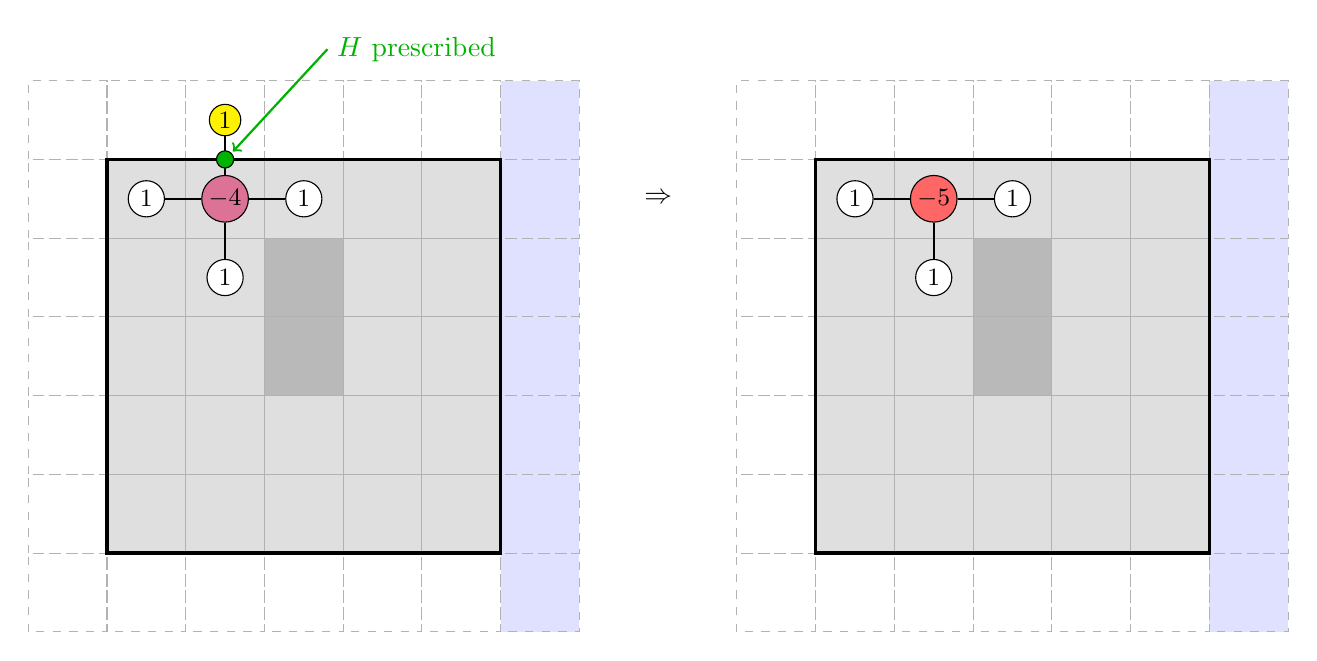
\begin{tikzpicture}[scale=1.0]

%-------------------------------------------------
% Styles
%-------------------------------------------------
\tikzset{
  grid/.style={draw=gray!60, dashed},
  gridint/.style={draw=gray!60},
  boundary/.style={draw=black, line width=1.2pt},
  gas/.style={fill=gray!25},
  solid/.style={fill=gray!55},
  one/.style={circle, draw, fill=white, inner sep=2pt},
  center_before/.style={circle, draw, fill=purple!55, inner sep=1.2pt},
  center_after/.style={circle, draw, fill=red!60, inner sep=1.2pt},
  ghostval/.style={circle, draw, fill=yellow, inner sep=1.4pt},
  bcval/.style={circle, draw, fill=green!70!black, inner sep=1.4pt}
}

%-------------------------------------------------
% LEFT PANEL
%-------------------------------------------------

% Light blue interpolated mesh boundary
\fill[blue!12] (6,0) rectangle (7,7);

% Dashed grid everywhere
\foreach \i in {0,...,6} {
  \foreach \j in {0,...,6} {
    \draw[grid] (\i,\j) rectangle ++(1,1);
  }
}

% Gas region (expanded so only one ghost layer)
\fill[gas] (1,1) rectangle (6,6);

% Solid obstruction
\fill[solid] (3,3) rectangle (4,5);

% Solid interior grid overlay
\foreach \i in {1,...,5} {
  \foreach \j in {1,...,5} {
    \draw[gridint] (\i,\j) rectangle ++(1,1);
  }
}

% Exterior boundary (thicker)
\draw[boundary] (1,1) rectangle (6,6);

%-------------------------------------------------
% Stencil coefficients (before BC)
%-------------------------------------------------
\node[one] (W) at (1.5,5.5) {\small $1$};
\node[one] (E) at (3.5,5.5) {\small $1$};
\node[one] (S) at (2.5,4.5) {\small $1$};

\node[center_before] (C) at (2.5,5.5) {\small $-4$};

% Ghost value (same size as off-diagonal)
\node[ghostval] (G) at (2.5,6.5) {\small $1$};

% BC annotation (same green everywhere)
\draw[->, thick, green!70!black] (3.8,7.4) -- (2.6,6.1);
\node[right, green!70!black] at (3.8,7.4) {$H$ prescribed};

%-------------------------------------------------
% Stencil connectivity lines
%-------------------------------------------------
\draw[black, thick] (C) -- (W);
\draw[black, thick] (C) -- (E);
\draw[black, thick] (C) -- (S);
\draw[black, thick] (C) -- (G);

% Dirichlet BC location
\node[bcval] (BC) at (2.5,6.0) {$\;$};


%-------------------------------------------------
% Arrow
%-------------------------------------------------
\node at (8,5.5) {$\Rightarrow$};

%-------------------------------------------------
% RIGHT PANEL
%-------------------------------------------------
\begin{scope}[xshift=9cm]

% Light blue interpolated mesh boundary
\fill[blue!12] (6,0) rectangle (7,7);

% Dashed grid
\foreach \i in {0,...,6} {
  \foreach \j in {0,...,6} {
    \draw[grid] (\i,\j) rectangle ++(1,1);
  }
}

% Gas region
\fill[gas] (1,1) rectangle (6,6);

% Solid obstruction
\fill[solid] (3,3) rectangle (4,5);

% Solid interior grid
\foreach \i in {1,...,5} {
  \foreach \j in {1,...,5} {
    \draw[gridint] (\i,\j) rectangle ++(1,1);
  }
}

% Exterior boundary
\draw[boundary] (1,1) rectangle (6,6);

% Stencil coefficients
\node[one] (W) at (1.5,5.5) {\small $1$};
\node[one] (E) at (3.5,5.5) {\small $1$};
\node[one] (S) at (2.5,4.5) {\small $1$};

\node[center_after] (C) at (2.5,5.5) {\small $-5$};

%-------------------------------------------------
% Stencil connectivity lines
%-------------------------------------------------
\draw[black, thick] (C) -- (W);
\draw[black, thick] (C) -- (E);
\draw[black, thick] (C) -- (S);

\end{scope}

\end{tikzpicture}
\caption{Imposition of a Dirichlet boundary condition using a single ghost cell in FDS. The ghost value is eliminated using the prescribed boundary value, resulting in a modification of the diagonal entry of the discrete Laplacian and the right hand side.}
\label{fig:dirichlet_bc_fds}
\end{figure}


\subsection*{Neumann Boundary Conditions}

Suppose we are on the left side boundary (refer to Fig.~\ref{fig:neumann_bc_fds}).  Then the first cell index is $i=1$ and the ghost cell is $i=0$, for a given $j$.  The normal gradient conditions are imposed by constraining the ghost cell such that
\begin{equation}
\left.\frac{\partial H}{\partial x}\right|_{\mathrm{BC},j} = \frac{H_{1,j}-H_{0,j}}{\delta x_0} \quad \Rightarrow \quad H_{0,j} = \left.\frac{\partial H}{\partial x}\right|_{\mathrm{BC},j} \delta x_0 + H_{1,j},
\end{equation}
where $\frac{\partial H}{\partial n}|_{\mathrm{BC},j}$ exactly controls the normal component of velocity at the boundary per Eqs.~(\ref{dbc}) and (\ref{dbc2}) in Sec.~\ref{ssub:solid_boundary_conditions}.  In this case, we are considering an external boundary, but later we will see that this same boundary condition can be applied to an internal solid obstruction leading to an unstructured pressure equation.  As can be seen, eliminating the ghost cell adds $1$ to the diagonal coefficient and the RHS is augmented in this case by
\begin{equation}
\mathrm{RHS}_{1,j} = b_{1,j} - \left.\frac{\partial H}{\partial x}\right|_{\mathrm{BC},j} \delta x_0 \, A_{W,j}
\end{equation}

\begin{figure}[h]
\centering
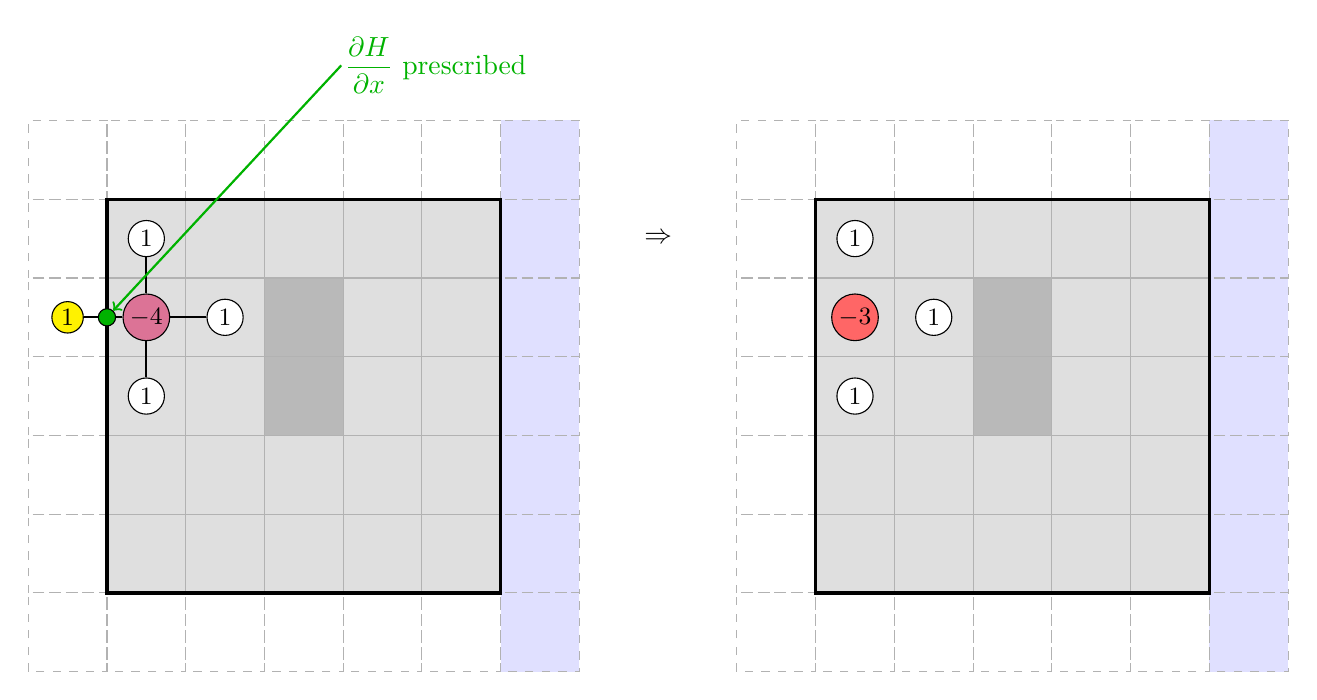
\begin{tikzpicture}[scale=1.0]

%-------------------------------------------------
% Styles (same as Dirichlet)
%-------------------------------------------------
\tikzset{
  grid/.style={draw=gray!60, dashed},
  gridint/.style={draw=gray!60},
  boundary/.style={draw=black, line width=1.2pt},
  gas/.style={fill=gray!25},
  solid/.style={fill=gray!55},
  one/.style={circle, draw, fill=white, inner sep=2pt},
  center_before/.style={circle, draw, fill=purple!55, inner sep=1.2pt},
  center_after/.style={circle, draw, fill=red!60, inner sep=1.2pt},
  ghostval/.style={circle, draw, fill=yellow, inner sep=1.4pt},
  bcval/.style={circle, draw, fill=green!70!black, inner sep=1.4pt}
}

%-------------------------------------------------
% LEFT PANEL (before elimination)
%-------------------------------------------------

% Light blue interpolated mesh boundary
\fill[blue!12] (6,0) rectangle (7,7);

% Dashed grid everywhere
\foreach \i in {0,...,6} {
  \foreach \j in {0,...,6} {
    \draw[grid] (\i,\j) rectangle ++(1,1);
  }
}

% Gas region
\fill[gas] (1,1) rectangle (6,6);

% Solid obstruction
\fill[solid] (3,3) rectangle (4,5);

% Solid interior grid overlay
\foreach \i in {1,...,5} {
  \foreach \j in {1,...,5} {
    \draw[gridint] (\i,\j) rectangle ++(1,1);
  }
}

% Exterior boundary
\draw[boundary] (1,1) rectangle (6,6);

%-------------------------------------------------
% Stencil coefficients (Neumann BC)
%-------------------------------------------------
\node[one] (E) at (2.5,4.5) {\small $1$};
\node[one] (N) at (1.5,5.5) {\small $1$};
\node[one] (S) at (1.5,3.5) {\small $1$};

\node[center_before] (C) at (1.5,4.5) {\small $-4$};

% Ghost value
\node[ghostval] (G) at (0.5,4.5) {\small $1$};

%-------------------------------------------------
% Stencil connectivity lines
%-------------------------------------------------
\draw[black, thick] (C) -- (E);
\draw[black, thick] (C) -- (N);
\draw[black, thick] (C) -- (S);
\draw[black, thick] (C) -- (G);

% Neumann BC location
\node[bcval] (BC) at (1.0,4.5) {$\;$};

% % BC annotation
% \draw[->, thick, green!70!black] (3.8,7.4) -- (2.6,6.1);
% \node[left, green!70!black] at (3.5,7.7)
% {$\displaystyle \frac{\partial H}{\partial x}\ \text{prescribed}$};

% BC annotation label (unchanged)
\node[green!70!black, anchor=west] (BCLabel)
  at (3.8,7.7) {$\displaystyle \; \frac{\partial H}{\partial x}\ \text{prescribed}$};

% Leader line: left, then slanted to BC dot
\draw[->, thick, green!70!black]
  ([xshift=5pt]BCLabel.west)
  -- ++(-0pt,0)
  -- (BC);


%-------------------------------------------------
% Arrow + explanation
%-------------------------------------------------
\node at (8,5.5) {$\Rightarrow$};

%-------------------------------------------------
% RIGHT PANEL (after elimination)
%-------------------------------------------------
\begin{scope}[xshift=9cm]

% Light blue interpolated mesh boundary
\fill[blue!12] (6,0) rectangle (7,7);

% Dashed grid
\foreach \i in {0,...,6} {
  \foreach \j in {0,...,6} {
    \draw[grid] (\i,\j) rectangle ++(1,1);
  }
}

% Gas region
\fill[gas] (1,1) rectangle (6,6);

% Solid obstruction
\fill[solid] (3,3) rectangle (4,5);

% Solid interior grid
\foreach \i in {1,...,5} {
  \foreach \j in {1,...,5} {
    \draw[gridint] (\i,\j) rectangle ++(1,1);
  }
}

% Exterior boundary
\draw[boundary] (1,1) rectangle (6,6);

% Stencil coefficients (after elimination)
\node[one] at (2.5,4.5) {\small $1$};
\node[one] at (1.5,5.5) {\small $1$};
\node[one] at (1.5,3.5) {\small $1$};

\node[center_after] at (1.5,4.5) {\small $-3$};

\end{scope}

\end{tikzpicture}
\caption{Imposition of a Neumann boundary condition using a ghost cell in FDS. The ghost value is defined to enforce a prescribed normal gradient at the boundary. Elimination of the ghost cell removes one neighbor contribution, resulting in a change of the diagonal entry of the discrete Laplacian from $-4$ to $-3$.  The RHS is augmented per Eq.~(X).}
\label{fig:neumann_bc_fds}
\end{figure}

%=============================================================================
\section{Solution Methods}
%=============================================================================

\subsection*{Fast Trigonometric (FFT) Solver}

On single, uniform, structured meshes with separable boundary conditions, the Poisson equation is solved using a fast trigonometric method based on discrete sine and cosine transforms. This approach exploits the separability of the Laplacian operator, yielding an $\mathcal{O}(N \log N)$ solution with minimal memory overhead.

The FFT solver is restricted to cases without internal boundaries or mesh
refinement.

\subsection*{Global Matrix Solver (UGLMAT / HYPRE)}

For general geometries involving mesh refinement, immersed boundaries, or multiple meshes, FDS assembles the global linear system and solves it using the UGLMAT framework, which interfaces with the HYPRE library.

The resulting matrix is sparse and symmetric, incorporates boundary conditions through local row modifications, and includes explicit coarse--fine coupling terms at refinement interfaces. Iterative solvers with multigrid preconditioning are used to obtain $H$, after which velocities are corrected locally on each mesh.

%=============================================================================
\section{Coarse--Fine Interface Consistency}
\label{sec:flux_matching_uglmat}
%=============================================================================

The guard cell interpolation and flux--matching procedure described below ensures that the discrete gradient $\nabla H$ used in the velocity update is consistent with the fluxes represented in the global Poisson matrix. This consistency is essential for maintaining velocity continuity across refinement interfaces when using the UGLMAT solver.

\subsection*{Geometry at Coarse-Fine Interface}

At a refinement interface, one coarse cell face connects to multiple fine cell faces. For a 2:1 refinement ratio in 3D, one coarse face connects to 4 fine faces (2$\times$2 arrangement).

\begin{figure}[h]
\centering
\begin{tikzpicture}[scale=1.2]
    % Coarse mesh cell
    \draw[thick] (0,0) rectangle (2,2);
    \node at (1,0.7) {$H_C$};
    \node at (1,-0.3) {Coarse Mesh};

    % Fine mesh cells (2x2)
    \draw[thick] (2.5,0) rectangle (3.5,1);
    \draw[thick] (2.5,1) rectangle (3.5,2);
    \draw[thick] (3.5,0) rectangle (4.5,1);
    \draw[thick] (3.5,1) rectangle (4.5,2);

    \node at (3,0.25) {$H_{F1}$};
    \node at (3,1.25) {$H_{F2}$};
    \node at (4,0.25) {$H_{F3}$};
    \node at (4,1.25) {$H_{F4}$};
    \node at (3.5,-0.3) {Fine Mesh};

    % Interface
    \draw[dashed, thick, red] (2.25,0) -- (2.25,2);
    \node[red] at (2.25,2.3) {Interface};

    % Cell centers
    \fill[blue] (1,1) circle (3pt);
    \fill[blue] (3,0.5) circle (2pt);
    \fill[blue] (3,1.5) circle (2pt);
    \fill[blue] (4,0.5) circle (2pt);
    \fill[blue] (4,1.5) circle (2pt);

    % Arrows showing flux coupling
    \draw[-{Stealth}, thick, green!60!black] (1.2,1) -- (2.8,0.5);
    \draw[-{Stealth}, thick, green!60!black] (1.2,1) -- (2.8,1.5);

    % Distances
    \draw[<->, gray] (1,-0.8) -- (2.25,-0.8);
    \node[gray] at (1.625,-1.1) {$\delta x_C/2$};
    \draw[<->, gray] (2.25,-0.8) -- (3,-0.8);
    \node[gray] at (2.625,-1.1) {$\delta x_F/2$};
\end{tikzpicture}
\caption{2D view of coarse-fine interface showing cell centroids (blue dots) and flux couplings (green arrows). The interface (red dashed line) separates the coarse mesh from the fine mesh.}
\label{fig:coarse_fine_interface}
\end{figure}

\section{Distance Calculation at Refinement Interfaces}

For a face at a refinement interface between a coarse cell $C$ and a fine cell $F$, the distance between cell centers is:
\begin{equation}
    \delta x_{CF} = \frac{\delta x_C}{2} + \frac{\delta x_F}{2}
    \label{eq:interface_distance}
\end{equation}
where $\Delta x_C$ and $\Delta x_F$ are the cell sizes in the normal direction.

The inverse distance used in the flux coefficient is:
\begin{equation}
    \text{IDX} = \frac{1}{\delta x_{CF}} = \frac{2}{\delta x_C + \delta x_F}
    \label{eq:idx}
\end{equation}

% \subsection{Area at Refinement Interfaces}

% When a coarse cell connects to multiple fine cells, each fine cell's face area $A_F$ will be smaller than the coarse cell's face area $A_C$. The effective coupling area is the \emph{minimum} of the two:
% \begin{equation}
%     A_{\text{eff}} = \min(A_C, A_F) = A_F
%     \label{eq:effective_area}
% \end{equation}

% This ensures that the flux through a fine cell's face is computed using the actual contact area, not the larger coarse cell area.

\subsection*{Flux Coupling Coefficient for Refinement Interface}

When a coarse cell connects to multiple fine cells, each fine cell's face area $A_F$ will be smaller than the coarse cell's face area $A_C$.  The coupling coefficient between coarse cell $C$ and fine cell $F_k$ is:
\begin{equation}
    B_{C,F_k} = \frac{A_{F_k}}{\frac{\delta x_C}{2} + \frac{\delta x_{F_k}}{2}}
    \label{eq:refinement_coupling}
\end{equation}

The total flux from the coarse cell is conserved:
\begin{equation}
    \sum_{k} B_{C,F_k} (H_{F_k} - H_C) = \text{total flux through coarse face}
    \label{eq:flux_conservation}
\end{equation}

%=============================================================================
\section{Guard Cell Interpolation for Consistent Gradients}
%=============================================================================

\subsection*{Problem Statement}

After solving the global pressure system, each mesh has the solution $H$ for its internal cells. However, to compute the pressure gradient $\nabla H$ at mesh boundaries consistently, guard cells need appropriate values of $H$.

At refinement interfaces, we have:
\begin{itemize}
    \item The coarse mesh guard cell overlaps multiple fine cells
    \item Simple copying would not preserve gradient continuity
    \item Flux matching requires cell center to center distance-weighted interpolation for cartesian grids.
\end{itemize}

\subsection*{Flux matched Interpolation}

\begin{figure}[h]
\centering
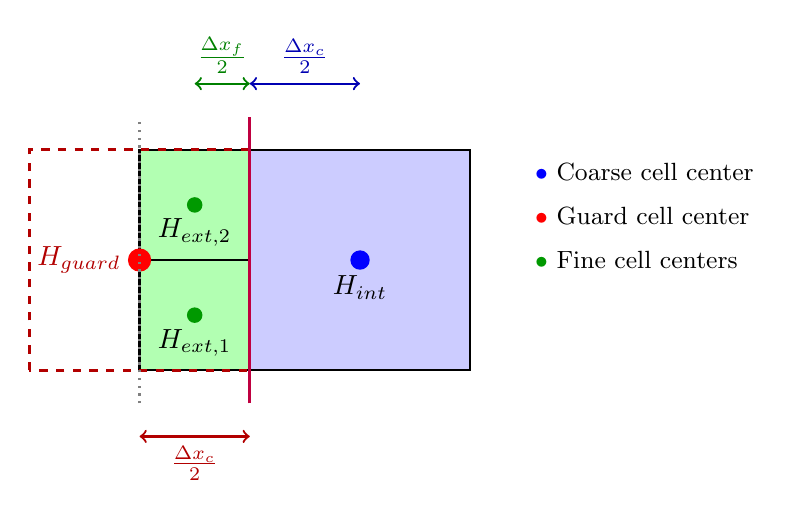
\begin{tikzpicture}[scale=1.4]
    % === COARSE MESH (right side) ===
    % Internal coarse cell (width = 2 units)
    \draw[thick, fill=blue!20] (0,0) rectangle (2,2);
    \node at (1,0.75) {$H_{int}$};
    \fill[blue] (1,1) circle (2.5pt);

    % === FINE MESH (2 cells at the interface, width = 1 unit = half coarse) ===
    \draw[thick, fill=green!30] (-1,0) rectangle (0,1);
    \draw[thick, fill=green!30] (-1,1) rectangle (0,2);

    % Fine cell labels and centers
    \node at (-0.5,0.25) {$H_{ext,1}$};
    \node at (-0.5,1.25) {$H_{ext,2}$};
    \fill[green!60!black] (-0.5,0.5) circle (2pt);
    \fill[green!60!black] (-0.5,1.5) circle (2pt);

    % === Guard cell of coarse mesh (dashed boundary, overlapping fine cells) ===
    \draw[very thick, dashed, red!70!black] (-2,0) rectangle (0,2);
    % Guard cell centroid at x=-1 (corresponds to left edge of fine cells)
    \fill[red] (-1,1) circle (3pt);
    \node[red!70!black] at (-1.55,1) {$H_{guard}$};

    % === Interface ===
    \draw[very thick, purple] (0,-0.3) -- (0,2.3);

    % === Distances ===
    % Coarse cell distance to face
    \draw[<->, blue!70!black, thick] (0,2.6) -- (1,2.6);
    \node[blue!70!black, above] at (0.5,2.6) {$\frac{\Delta x_c}{2}$};

    % Fine cell distance to face (half of fine cell width)
    \draw[<->, green!50!black, thick] (-0.5,2.6) -- (0,2.6);
    \node[green!50!black, above] at (-0.25,2.6) {$\frac{\Delta x_f}{2}$};

    % Guard cell center distance from interface
    \draw[<->, red!70!black, thick] (-1,-0.6) -- (0,-0.6);
    \node[red!70!black, below] at (-0.5,-0.6) {$\frac{\Delta x_c}{2}$};

    % Show fine cell edge aligns with guard centroid
    \draw[dotted, gray, thick] (-1,-0.3) -- (-1,2.3);

    % === Legend ===
    \node[anchor=west] at (2.5,1.8) {\small \textcolor{blue}{$\bullet$} Coarse cell center};
    \node[anchor=west] at (2.5,1.4) {\small \textcolor{red}{$\bullet$} Guard cell center};
    \node[anchor=west] at (2.5,1.0) {\small \textcolor{green!60!black}{$\bullet$} Fine cell centers};

\end{tikzpicture}
\caption{Guard cell interpolation at 2:1 refinement interface. The fine cells have half the width
of the coarse cell ($\Delta x_f = \Delta x_c/2$). The coarse guard cell (red dashed boundary)
overlaps two fine cells. The guard cell centroid (red dot) is located at $\Delta x_c/2$ from the
interface, which corresponds to the left edge of the fine cells (gray dotted line).}
\label{fig:guard_interpolation}
\end{figure}

The algorithm proceeds as follows:

\begin{enumerate}
    \item \textbf{Average external cell values}: For cells in the neighbor mesh range, compute:
    \begin{equation}
        \bar{H}_{ext} = \frac{1}{N_{ext}} \sum_{k=1}^{N_{ext}} H_{ext,k}
        \label{eq:h_ext_mean}
    \end{equation}
    Only include cells where the external wall cell type is \ct{INTERPOLATED_BOUNDARY}. Note this is equivalent to area averaging the solution for structured cartesian grids.

    \item \textbf{Interpolate to face}: Using distance weighting:
    \begin{equation}
        H_{face} = w_{int} H_{int} + w_{ext} \bar{H}_{ext}
        \label{eq:h_face}
    \end{equation}
    where the weights are:
    \begin{align}
        w_{int} &= \frac{\delta x_{ext}}{\delta x_{int} + \delta x_{ext}} \\
        w_{ext} &= \frac{\delta x_{int}}{\delta x_{int} + \delta x_{ext}}
        \label{eq:weights}
    \end{align}

    \item \textbf{Extrapolate to guard cell center}: The guard cell is located at distance $\delta x_{int}/2$ from the face on the external side:
    \begin{equation}
        H_{guard} = H_{int} + 2(H_{face} - H_{int})
        \label{eq:h_guard}
    \end{equation}
\end{enumerate}

This ensures that the gradient computed in the internal mesh:
\begin{equation}
    \frac{\partial H}{\partial x} \approx \frac{H_{int} - H_{guard}}{\delta x_{int}}
    \label{eq:gradient_internal}
\end{equation}
is consistent with the flux used in the pressure matrix. Note that this scheme works both for the fine and coarse sides in structured cartesian refined grids, leading to the coarse side having the area average of the gradient values computed from the fine side. This leads to matching velocities in the projection, provided initial velocities and forces are flux matched.


\end{document}
